\documentclass{article}

% if you need to pass options to natbib, use, e.g.:
    \PassOptionsToPackage{numbers, compress}{natbib}
% before loading neurips_2026

% The authors should use one of these tracks.
% Before accepting by the NeurIPS conference, select one of the options below.
% 0. "default" for submission

\usepackage{neurips_2026}
% the "default" option is equal to the "main" option, which is used for the Main Track with double-blind reviewing.
% 1. "main" option is used for the Main Track
%  \usepackage[main]{neurips_2026}
% 2. "position" option is used for the Position Paper Track
%  \usepackage[position]{neurips_2026}
% 3. "eandd" option is used for the Evaluations & Datasets Track
 % \usepackage[eandd]{neurips_2026}
 % if you need to opt-in for a single-blind submission in the E&D track:
 %\usepackage[eandd, nonanonymous]{neurips_2026}
% 4. "creativeai" option is used for the Creative AI Track
%  \usepackage[creativeai]{neurips_2026}
% 5. "sglblindworkshop" option is used for the Workshop with single-blind reviewing
 % \usepackage[sglblindworkshop]{neurips_2026}
% 6. "dblblindworkshop" option is used for the Workshop with double-blind reviewing
%  \usepackage[dblblindworkshop]{neurips_2026}

% After being accepted, the authors should add "final" behind the track to compile a camera-ready version.
% 1. Main Track
 % \usepackage[main, final]{neurips_2026}
% 2. Position Paper Track
%  \usepackage[position, final]{neurips_2026}
% 3. Evaluations & Datasets Track
 % \usepackage[eandd, final]{neurips_2026}
% 4. Creative AI Track
%  \usepackage[creativeai, final]{neurips_2026}
% 5. Workshop with single-blind reviewing
%  \usepackage[sglblindworkshop, final]{neurips_2026}
% 6. Workshop with double-blind reviewing
%  \usepackage[dblblindworkshop, final]{neurips_2026}
% Note. For the workshop paper template, both \title{} and \workshoptitle{} are required, with the former indicating the paper title shown in the title and the latter indicating the workshop title displayed in the footnote.
% For workshops (5., 6.), the authors should add the name of the workshop, "\workshoptitle" command is used to set the workshop title.
% \workshoptitle{WORKSHOP TITLE}

% "preprint" option is used for arXiv or other preprint submissions
 % \usepackage[preprint]{neurips_2026}

% to avoid loading the natbib package, add option nonatbib:
%    \usepackage[nonatbib]{neurips_2026}

\usepackage[utf8]{inputenc} % allow utf-8 input
\usepackage[T1]{fontenc}    % use 8-bit T1 fonts
\usepackage{hyperref}       % hyperlinks
\usepackage{url}            % simple URL typesetting
\usepackage{booktabs}       % professional-quality tables
\usepackage{amsfonts}       % blackboard math symbols
\usepackage{nicefrac}       % compact symbols for 1/2, etc.
\usepackage{microtype}      % microtypography
\usepackage{xcolor}         % colors
\usepackage{placeins}
% 补充：
\usepackage{graphicx}
\usepackage{subcaption}
\usepackage{amsmath}
\usepackage{amssymb}
\usepackage{mathtools}
\usepackage{amsthm}

\usepackage{CJKutf8}
\newcommand{\cn}[1]{\begin{CJK*}{UTF8}{bsmi}#1\end{CJK*}}
\newcommand{\cg}[1]{\begin{CJK*}{UTF8}{gbsn}#1\end{CJK*}}

\usepackage{enumitem}

\usepackage{pifont} % 提供 \ding{51}, \ding{55} (对钩和叉号)

\usepackage[table]{xcolor}
\usepackage{algorithm}    % 提供 algorithm 浮动体环境
\usepackage{algorithmic}  % 提供 algorithmic 环境和 \REQUIRE/\ENSURE/\STATE 等命令
\usepackage{wrapfig}

\usepackage{multirow}

\usepackage{titletoc} % 用于附录目录

% 放在导言区（\begin{document}之前），必须已加载xcolor包
\usepackage{xcolor}
% 【完美适配wrapfigure窄环境】无空行、无溢出、行号正常、全文档通用
\newcommand{\stageheader}[1]{%
  \STATE\hspace*{-\fboxsep}% 自带\STATE，禁止额外加\STATE！结尾加%消除隐形空格
  \colorbox{gray!20}{%
    \makebox[\dimexpr\linewidth\relax][l]{% 宽度严格等于算法文本可用宽度，无溢出
      \hspace*{\fboxsep}\textit{// #1}\hspace*{\linewidth-\widthof{\textit{// #1}}-2\fboxsep}% 文字左对齐，灰色撑满整行
    }%
  }%
  \hspace*{-\fboxsep}% 结尾加%消除隐形空格
}

% Note. For the workshop paper template, both \title{} and \workshoptitle{} are required, with the former indicating the paper title shown in the title and the latter indicating the workshop title displayed in the footnote. 
\title{A Unified Manifold Framework for Modeling Chinese Script Evolution with Application to Oracle Bone Decipherment}


% The \author macro works with any number of authors. There are two commands
% used to separate the names and addresses of multiple authors: \And and \AND.
%
% Using \And between authors leaves it to LaTeX to determine where to break the
% lines. Using \AND forces a line break at that point. So, if LaTeX puts 3 of 4
% authors names on the first line, and the last on the second line, try using
% \AND instead of \And before the third author name.


\author{%
  David S.~Hippocampus\thanks{Use footnote for providing further information
    about author (webpage, alternative address)---\emph{not} for acknowledging
    funding agencies.} \\
  Department of Computer Science\\
  Cranberry-Lemon University\\
  Pittsburgh, PA 15213 \\
  \texttt{hippo@cs.cranberry-lemon.edu} \\
  % examples of more authors
  % \And
  % Coauthor \\
  % Affiliation \\
  % Address \\
  % \texttt{email} \\
  % \AND
  % Coauthor \\
  % Affiliation \\
  % Address \\
  % \texttt{email} \\
  % \And
  % Coauthor \\
  % Affiliation \\
  % Address \\
  % \texttt{email} \\
  % \And
  % Coauthor \\
  % Affiliation \\
  % Address \\
  % \texttt{email} \\
}

\begin{document}


\maketitle


% \begin{abstract}
%     Of the approximately 4,500 Oracle Bone Inscription (OBI) characters discovered from the Shang dynasty, only about 1,600 have been deciphered. 
%     Existing computational methods mainly compute the similarity between OBI and single historical period characters independently. 
%     However, during the evolution of Chinese characters, significant structural or semantic changes often occur in uncertain dynasties. Relying solely on a single dynasty for reference leads to numerous deciphering errors.
%     Therefore, we propose the \textbf{Manifold-based Script Evolution Framework (MSEF)}, the first unified framework that models the evolution series (OBI, Bronze, Seal, Clerical, Regular) of Chinese characters as the continual evolution of a manifold space.
%     MSEF represents each character as an era-specific manifold point and learns continuous inter-era transition rules via Neural Ordinary Differential Equations. Both manifold space and transition dynamics can be trained end-to-end through character evolution pairs across any two eras.
%     To support this training scheme, we construct the first unified cross-era dataset with \textbf{fine-grained temporal and regional granularity}.
%     Based on MSEF, we propose the \textbf{Cascaded Bidirectional Evolutionary Decipherment (CBED)} algorithm, where forward predictions recall potential candidates and backward consistency checking filters false matches, effectively avoiding errors caused by single-dynasty comparisons.
%     % 提及附录pre和post
%     To ground our approach, we provide a rigorous pre-exploratory diagnosis that theoretically derives the necessity of continuous manifold dynamics by exposing the structural bottlenecks of existing discrete paradigms. Furthermore, comprehensive post-analysis via mechanistic interpretability reveals that MSEF autonomously learns evolutionary laws and information-routing circuits that closely align with human paleographic cognition.
%     Experiments on three commonly used benchmarks and our dataset demonstrate that MSEF achieves state-of-the-art performance among all current oracle deciphering algorithms. This work opens the possibility of using continuous manifold dynamics in cross-era paleographic decipherment. Dataset and code are released through our project page \url{https://icml26-oracle.github.io/}.
% \end{abstract}


\begin{abstract}
    Of the approximately 4,500 Oracle Bone Inscription (OBI) characters discovered from the Shang dynasty, only about 1,600 have been deciphered. 
    Existing computational methods mainly compute the similarity between OBI and single historical period characters independently. 
    However, during the evolution of Chinese characters, significant structural or semantic changes often occur in uncertain dynasties. Relying solely on a single dynasty for reference leads to numerous deciphering errors.
    Therefore, we propose the \textbf{Manifold-based Script Evolution Framework (MSEF)}, the first unified framework that models the evolution series (OBI, Bronze, Seal, Clerical, Regular) of Chinese characters as the continual evolution of a manifold space.
    MSEF represents each character as an era-specific manifold point and learns continuous inter-era transition rules via Neural Ordinary Differential Equations. Both manifold space and transition dynamics can be trained end-to-end through character evolution pairs across any two eras.
    To support this training scheme, we construct the first unified cross-era dataset with \textbf{fine-grained temporal and regional granularity}.
    Based on MSEF, we propose the \textbf{Cascaded Bidirectional Evolutionary Decipherment (CBED)} algorithm, where forward predictions recall potential candidates and backward consistency checking filters false matches, effectively avoiding errors caused by single-dynasty comparisons.
    To ground our approach, we provide a pre-exploratory diagnosis of existing generative and retrieval paradigms, showing why continuous manifold dynamics are well suited for fragmented cross-era script data. We further conduct mechanistic post-analysis, showing that the learned representations and transition dynamics capture patterns consistent with known paleographic transformations.
    Experiments on three commonly used benchmarks and our dataset demonstrate that MSEF achieves state-of-the-art performance among current oracle deciphering algorithms. This work opens the possibility of using continuous manifold dynamics in cross-era paleographic decipherment. Dataset and code are released through our project page \url{https://neurips26-oracle.github.io/}.
\end{abstract}




% \textbf{72.5\% top-1 accuracy}, outperforming the state-of-the-art OracleAgent by 9.7 percentage points.% ($p < 0.01$).
% could leverage the rich history cross-era correspondences spanning the complete evolution from OBI to modern Chinese characters series. 
% Finally, In order to train MSEF,

% models all five historical period characters evolution rules within a single mathematical structure. 


%%%%%%%%%%%%%%%%%%%%%%%%%%%%%%% introduction %%%%%%%%%%%%%%%%%%%%%
% \item We propose the first unified Manifold-based Script Evolution Framework (MSEF) which could model the evolution series(OBI, Bronze, Seal, Clerical, Regular) of Chinese characters as the continual evolution of a manifold space. Such framework contain a manifold net for represent the period, neural ode for represent the period transition, suvival net for represent the Discontinuity of Chinese Characters.
% \item We construct and opensource the first unified cross-era chinese oracle dataset which could support train the MSEF.
% % and facilitates training on incomplete chains (yielding a 9$\times$ data expansion).
% \item We introduce a Cascaded Bidirectional Evolutional Decipherment(CBED) mechanism that employs forward cascaded retrieval with backward verification, providing temporal consistency validation. Such mechanism could fully leverage the potential of MSEF in cryptanalysis tasks
%%%%%%%%%%%%%%%%%%%%%%%%%%%%%%%%%%%%%%%%%%%%%%%%%%%%%%%%%%%%%%%%%%%%%%%%%%%%%%%%%%%%
% , integrating three authoritative databases. 


% This formulation enables two key capabilities: (1) 

% expanding usable data from $\sim$1500 complete chains to $\sim$13,700 partial pairs (9$\times$ increase), and 

%%%%%%%%%%%%%%%%%%%%%%%%%%%%%%%%%%%%%%%%%%%%%%%%%%%%%%%%%%

% However, computational approaches \cite{gao2022image} face a fundamental data bottleneck \cite{diao2025ancient, wang2024puzzle}. As Figure~\ref{fig:data_stats} illustrates, of the 4,500 OBI characters, merely $\sim$1500 possess complete evolution chains across five historical periods. 


% The emergence of modern AI technologies presents a novel frontier for OBI decipherment, challenging traditional NLP methods that rely heavily on large textual corpora, a luxury not afforded by historical languages. Computational approaches to OBI decipherment \cite{gao2022image} face a fundamental data bottleneck \cite{diao2025ancient, wang2024puzzle}. As Figure~\ref{fig:data_stats} illustrates, of the 4,500 OBI characters, merely $\sim$1500 possess complete evolution chains across all five historical periods. This severe fragmentation has forced existing methods to model each era-pair independently, discarding the abundant partial correspondences that exist between non-adjacent periods \cite{guo2015building, zhang2019oracle, li2023towards}.

% Current approaches generally fall into two categories: image-based methods that focus on recognition \cite{meng2018recognition, hu2024component} or generation \cite{chang2022sundial, li2023diff}, and cross-modal methods that bridge visual and semantic information \cite{wu2025cross, chen2024obi}. 
% Despite their diversity, these methods share three limitations. \textbf{First}, they suffer from fragmented modeling, where training separate models for each era pair inevitably wastes abundant partial correspondences. \textbf{Second}, they lack evolutionary compatibility. Prior voting-based approaches ignore distinct character lifespans, treating all eras as equally valid. This forces noisy comparisons between incompatible periods, as existing methods lack the continuous temporal mechanism to discern valid pairs. \textbf{Finally}, most existing frameworks are limited to unidirectional prediction, with no mechanism to verify whether the predictions remain temporally consistent in both directions.

% However, the evolutionary dynamics are crucial because the morphological trajectory of Chinese characters is highly non-uniform and character-specific. Some glyphs transition smoothly from OBI to Bronze but undergo drastic structural mutations in the Seal script, while others remain stable until the Clerical transformation. 

% A robust decipherment framework must therefore possess the \textit{evolutionary compatibility} to adaptively determine which specific era-pairs provide valid evidence for each individual character.




% Consider how the character ``ox'' evolved, its pictographic OBI form, which depicts an ox head with horns, gradually simplified through Bronze and Seal scripts, eventually becoming the abstract modern form ``\cg{牛}''. This transformation follows systematic patterns---structural components are preserved \cite{xigui2000chinese} while stylistic features evolve smoothly. This observation motivates modeling script evolution as continuous flow through a shared geometric space \cite{bottero1996origin, meilua2024manifold}, where each historical period defines a distinct coordinate system but the underlying structure remains unified.

% We propose \textbf{Manifold-based Script Evolution Framework (MSEF)}, the first unified computational framework addressing all three limitations above. MSEF models the complete evolutionary trajectory as a single learnable dynamical system. Each historical era maps to a distinct manifold space, and inter-period transitions follow continuous, invertible flows governed by Neural Ordinary Differential Equations (Neural ODE) \cite{chen2018neural, rubanova2019latent}.

% We propose \textbf{Manifold-based Script Evolution Framework (MSEF)} to model script evolution as continuous flow through a shared geometric space \cite{bottero1996origin, meilua2024manifold}, where each historical period maps to a distinct manifold space defines a distinct coordinate system and inter-period transitions follow continuous, invertible flows governed by Neural Ordinary Differential Equations (Neural ODE), but the underlying structure remains unified \cite{chen2018neural, rubanova2019latent}.

% We propose \textbf{Manifold-based Script Evolution Framework (MSEF)} to model script evolution as a continuous flow through a shared geometric space \cite{bottero1996origin, meilua2024manifold}. In this framework, each historical period defines a distinct coordinate system, while inter-period transitions are governed by continuous, invertible Neural Ordinary Differential Equations (Neural ODE) \cite{chen2018neural, rubanova2019latent}, ensuring a unified underlying structure.

% Distinguishing itself from prior generative approaches, MSEF is the first to explicitly formulate and benchmark OBI decipherment as a large-scale discriminative classification task.

% This unified formulation yields two critical advantages. First, \textbf{training on incomplete chains}: since our manifold network is time-conditioned, any corresponding character pair across any two eras provides valid supervision, expanding usable data from $\sim$1500 to $\sim$13,700 pairs. Second, \textbf{bidirectional verification}: because our flow is invertible, we trace candidates backward through time and verify whether their predicted OBI features match the query. Figure~\ref{fig:overview} illustrates this cascaded bidirectional decipherment process.
% 我们的的方法
% We first model the  as the evolution of a manifold space.

% model the evolution series(OBI, Bronze, Seal, Clerical, Regular) of Chinese characters as the continual evolution of a manifold space.
% % models all five historical period characters evolution rules within a single mathematical structure. 
% MSEF represents each era each character as an era-specific manifold space point and learns continuous a unified character point inter-era point transition rules via Neural Ordinary Differential Equations. Both the unified manifold space and inter-era transitions neural ode could be training through different character evolution pairs (era1, era2) in an end-to-end manner, which could then used to predict different character evolution trace such as predict next-era the character structure. So based on MSEF, We proposed Bidirectional Evolutional Decipherment(BED) algorithm where forward predictions could recall all potential character candidates and backward consistency checking could filter all false samples further. Such way could effectively avoids decryption errors caused by comparisons limited to a single dynasty.
% % could leverage the rich history cross-era correspondences spanning the complete evolution from OBI to modern Chinese characters series. 
% Finally, In order to train MSEF, We construct the first unified cross-era dataset distinguished by \textbf{fine-grained temporal and regional granularity}.
% Experiments on both 3 Commonly used datasets and our own datasets demonstrate that MSEF achieves \textbf{72.5\% top-1 accuracy}, outperforming the state-of-the-art OracleAgent by 9.7 percentage points.% ($p < 0.01$).
% This unified formulation yields a critical advantage in training on incomplete chains. Since our manifold network is time-conditioned, any corresponding character pair across any two eras provides valid supervision.
% , expanding usable data from $\sim$1,500 complete chains to 
% and facilitates training on incomplete chains (yielding a 9$\times$ data expansion).
% Extensive experiments demonstrate that MSEF achieves state-of-the-art results with 80\% top-1 accuracy, significantly outperforming the previous best method, OracleAgent, by 17.2 points ($p < 0.01$).
%%%%%%%%%%%%%%%%%%%%%%%%%%%%%%%%%%%%%%%%%%%%%%%%%%%%%%%%%%%


\section{Introduction}
% 任务介绍，任务很难
Oracle Bone Inscription (OBI) is a cornerstone in the annals of linguistic history, predating many established writing systems \cite{gil2020will}. Chinese characters evolve over three millennia from Shang dynasty OBI, through Zhou dynasty Bronze Inscriptions, Qin dynasty Seal Script, Han dynasty Clerical Script, to modern Regular Script. Figure ~\ref{fig:evolution} illustrates the evolution process. Among the approximately 4,500 OBI characters discovered, only about 1,600 (35.6\%) have been deciphered \cite{keightley1985sources, li2020hwobc}. Deciphering the remaining $\sim$2,900 characters would unlock invaluable insights into early Chinese civilization \cite{wang2024dataset}, yet this process often takes years per character due to the need to thoroughly examine structural features and semantic patterns across different eras.

% 现有方法介绍，介绍的时候分类方式就按照缺点来分类。
The emergence of AI technologies presents a novel frontier for OBI deciphering. Current approaches generally fall into two categories: (1) compare OBI with modern simplified Chinese by image retrieval \cite{meng2018recognition, hu2024component} or generate modern simplified Chinese\cite{chang2022sundial, li2023diff}, sometimes incorporating semantic information \cite{chen2024obi}; and (2) compare OBI with other historical scripts such as Bronze \cite{wu2025cross}.


% {r} 表示图片靠右对齐 (right)
% {0.4\textwidth} 是分配给这个图片区域的整体宽度，你可以根据需要调整大小
\begin{wrapfigure}{r}{0.7\textwidth}
  \centering
  % 注意：这里的宽度改为 \linewidth，让图片填满你上面设置的 0.4\textwidth 的区域
  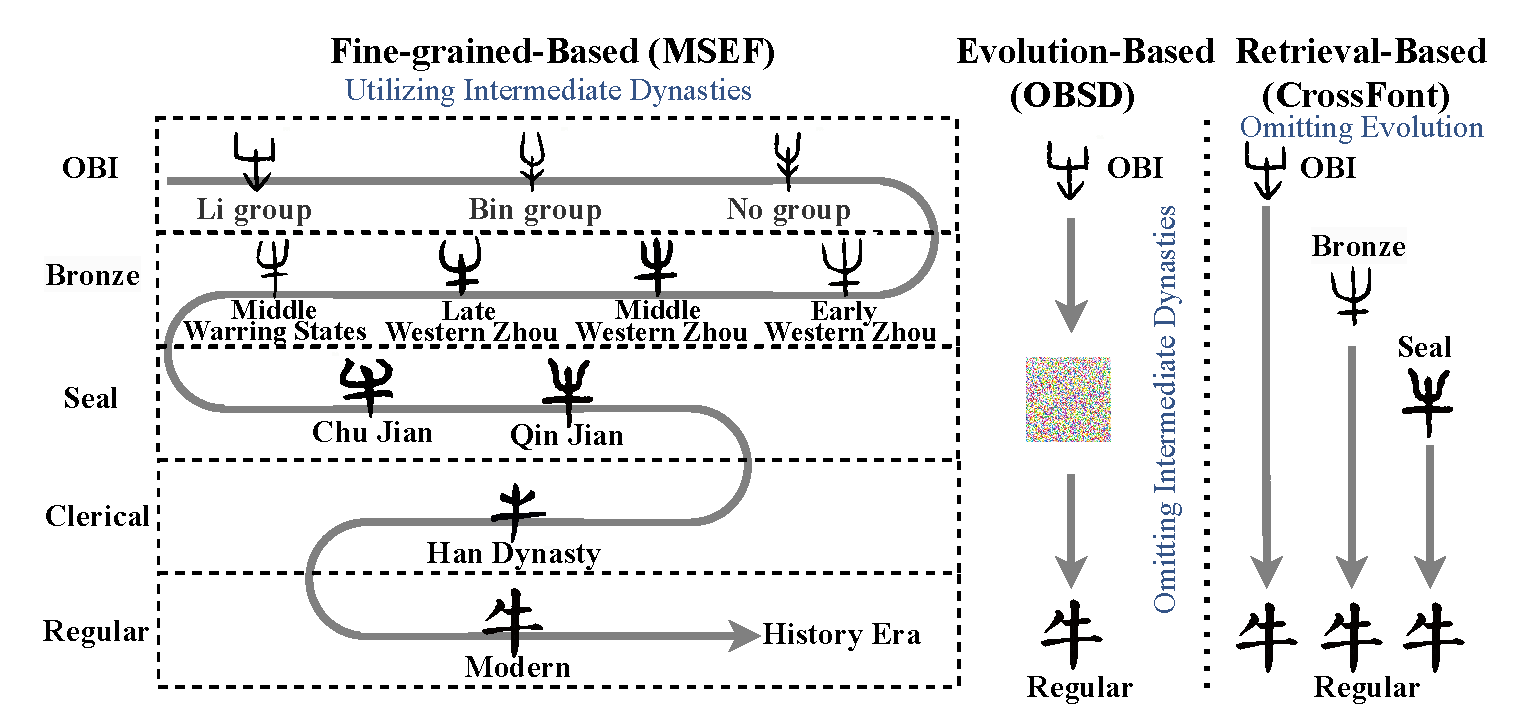
\includegraphics[width=\linewidth]{Evolution.pdf}
  \caption{\textbf{Evolution of Chinese Script.} Taking the character ``Ox'' as an example, this figure demonstrates the evolution of Chinese characters across five historical periods. 
  This character underwent a significant morphological change in early bronze script, then later reverted to a form similar to its oracle bone appearance. Conventional retrieval methods based solely on bronze script would incorrectly judge the similarity as low, leading to decipherment errors. Accurate decipherment requires considering the character's evolution across multiple dynasties and their temporal dependencies.}
  \label{fig:evolution}
\end{wrapfigure}


% 现有的方法方法存在一些问题：没有考虑时序演化信息
% 简体汉字问题
The first type attempts direct mappings from OBI-to-modern, ignoring critical intermediate stages \cite{guo2015building, zhang2019oracle, li2023towards}. This proves to be ineffective for characters that underwent major transformations during specific dynasties.
% cross-font问题
The second type, while incorporating multi-era comparisons, treats historical scripts as independent static sets. For instance, CrossFont \cite{wu2025cross} processes multi-era data but fails to model temporal evolutionary dynamics explicitly, which often leads to making it difficult to recall fonts that underwent drastic changes during the dynasties being compared.
% 文字生命周期问题
Moreover, character lifespans vary significantly—certain OBI glyphs became extinct before the Bronze era—yet approaches that force comparisons across all periods inevitably introduce noise. The current approach does not solve this issue either, but instead proceeds with decipherment under the assumption that all oracle bone inscriptions have survived to the present day.
% 一句话：这些破译方法没有考虑时序信息
% These limitations arise because existing methods fail to account for the evolutionary patterns of Chinese characters.
In such a situation, it is crucial to develop a method that fully accounts for the evolutionary patterns of the oracle bone script and considers decipherment across all dynasties.
% To address these issues, 
So we propose the \textbf{Manifold-based Script Evolution Framework (MSEF)} \cite{bottero1996origin, meilua2024manifold}, modeling character evolution as continuous flow through a shared manifold space directly.
% 摘要里的介绍进行细化：
Specifically, (1) under MSEF, each historical period defines a distinct high-dimensional coordinate system where each character corresponds to a unique point. Inter-period transitions are governed by continuous, invertible Neural Ordinary Differential Equations (Neural ODE) \cite{chen2018neural, rubanova2019latent}. (2) We implement the manifold using a time-conditioned transformer mapping feature vectors to coordinates, with a spectrally-normalized network for the ODE ensuring continuous transitions. (3) Furthermore, we additionally introduce a survival network that predicts character extinction probability across dynasties.

To support MSEF training, we \textbf{construct a fine-grained dataset} containing 1,500 complete evolution chains and $\sim$13,700 pairwise combinations. Based on trained MSEF, we propose \textbf{Cascaded Bidirectional Evolutionary Decipherment (CBED)}, which performs forward cascade retrieval with a survival mechanism to terminate extinct paths, followed by backward verification via inverse ODE flows with step-wise pruning for evolutionary consistency.

% Beyond empirical performance, this paper emphasizes rigorous theoretical derivation and mechanistic transparency. In our pre-exploratory analysis (Appendix ~\ref{sec:pre}), we systematically diagnose the failure modes of existing generative and retrieval paradigms, proving that incremental patches cannot overcome their lack of continuous historical priors, thereby mathematically necessitating our Neural ODE manifold approach. Once trained, we open the ``black box'' of MSEF through extensive post-analysis (Appendix ~\ref{sec:post_analysis}). By employing causal patching, attention circuit analysis, and latent vector arithmetic, we demonstrate that the model does not merely memorize visual patterns, but rather internalizes the sociolinguistic natural selection and morphodynamic laws of Chinese script evolution, developing emergent information-routing circuits that closely mirror human expert cognition.

% The final architecture proposed in this paper is the culmination of rigorous theoretical derivation and systematic experimental exploration. In our pre-exploratory analysis (Appendix~\ref{sec:pre}), we delineate this research trajectory: First, we systematically diagnose existing generative and retrieval paradigms, revealing that their failure modes stem from a fundamental inability to model the intermediate stages of script evolution. Second, we return to first principles to establish a theoretical foundation, defining character evolution as a duality of an invariant semantic core and a variant visual surface driven by continuous socio-cultural pressures. Third, we conduct a large-scale quantitative analysis to discover four distinct morphological evolution clusters, empirically mapping baseline vulnerabilities directly to non-monotone and abrupt historical transitions. Finally, we explore alternative solutions, demonstrating that attempting to salvage these tasks through incremental patches or discrete rule-based expert systems inevitably leads to unbreakable performance ceilings and combinatorial explosions. These sequential diagnostic findings mathematically necessitate our proposed MSEF powered by Neural ODEs.

% Although extensive quantitative evaluations demonstrate the superior capabilities of MSEF, the fully trained model inherently presents as a complex black box. To rigorously comprehend its underlying mechanisms and ascertain why it achieves such robust decipherment performance, we conduct an extensive mechanistic post-analysis (Appendix~\ref{sec:post_analysis}). Our framework design centers on several critical components, notably the continuous manifold character representations, the Neural ODE inter-era transition dynamics, and the survival net. By employing mechanistic interpretability visualizations, specifically causal saliency maps and attention circuit diagrams, we conduct fine-grained visual and experimental analyses on each of these modules. These visualizations rigorously prove the efficacy of our proposed components, demonstrating that the model does not merely memorize visual patterns, but rather develops emergent information-routing circuits that deeply internalize the sociolinguistic natural selection and morphodynamic laws of Chinese script evolution.

The final architecture proposed in this paper is the culmination of systematic theoretical derivation and experimental exploration. In our pre-exploratory analysis (Appendix~\ref{sec:pre}), we delineate this research trajectory: First, we systematically diagnose existing generative and retrieval paradigms, revealing that their failure modes stem from a fundamental inability to model intermediate stages of script evolution. Second, we return to first principles to define character evolution as a duality of an invariant semantic core and a variant visual surface driven by continuous socio-cultural pressures. Third, we conduct a quantitative analysis to identify distinct morphological evolution clusters, empirically mapping baseline vulnerabilities to non-monotone and abrupt historical transitions. Finally, we examine alternative solutions, showing that incremental patches or discrete rule-based expert systems face clear performance and scalability limitations. These diagnostic findings motivate our proposed MSEF powered by Neural ODEs.

Although extensive quantitative evaluations demonstrate the superior capabilities of MSEF, the fully trained model inherently presents as a complex black box. To better understand its underlying mechanisms and why it achieves robust decipherment performance, we conduct a mechanistic post-analysis (Appendix~\ref{sec:post_analysis}). Our framework design centers on several critical components, notably the continuous manifold character representations, the Neural ODE inter-era transition dynamics, and the survival net. By employing mechanistic interpretability visualizations, including causal saliency maps and attention circuit diagrams, we conduct fine-grained analyses on each of these modules. These analyses provide evidence that the model does not merely memorize visual patterns, but captures information-routing patterns and morphodynamic regularities consistent with known paleographic transformations.

Our contributions are:
\begin{itemize}[leftmargin=*,itemsep=2pt,topsep=2pt]
\item We propose a Manifold-based Script Evolution Framework (MSEF) which could model the evolution series(OBI, Bronze, Seal, Clerical, Regular) of Chinese characters as the continual evolution of a manifold space. Such framework contains a manifold net for representing the period, neural ode for representing the period transition, and survival net for representing the Discontinuity of Chinese Characters.
\item We construct and opensource the first unified cross-era oracle dataset which could support training the MSEF.
\item We introduce a Cascaded Bidirectional Evolutionary Decipherment (CBED) mechanism that employs forward cascaded retrieval with backward verification, providing temporal consistency validation. Such a mechanism could fully leverage the potential of MSEF chinese character evolution knowledge in deciphering oracle bone task.
\item  Experiments on both 3 Commonly used datasets and our own datasets demonstrate that MSEF achieves the state-of-the-art among all currnet oracle deciphering algorithms.
\end{itemize}
% \section{Introduction}
% % 任务介绍，任务很难
% The Oracle Bone Inscription (OBI) is a cornerstone in the annals of linguistic history, predating many established writing systems \cite{gil2020will}. Chinese characters evolve over three millennia from Shang dynasty OBI, through Zhou dynasty Bronze Inscriptions, Qin dynasty Seal Script, Han dynasty Clerical Script, to modern Regular Script. Among the approximately 4,500 discovered OBI characters, only about 1,600 (35.6\%) have been deciphered \cite{keightley1985sources, li2020hwobc}. Deciphering the remaining $\sim$2,900 characters would unlock invaluable insights into early Chinese civilization \cite{wang2024dataset}. Because some undeciphered characters may not have survived into modern times, and because deciphering certain characters requires archaeologists to thoroughly examine the structural features and semantic patterns across different eras, fully demonstrating the evolutionary characteristics of a character before it can be definitively declared deciphered. This process often takes years to complete for a single character.

% % 现有方法介绍，介绍的时候分类方式就按照缺点来分类。
% The emergence of AI technologies presents a novel frontier for OBI decipherment. Current AI approaches generally fall into two categories: 1. Compare Oracle Character with Modern Simplified Chinese. Some methods focused on use image retrieve way to recognition and recall the related character\cite{meng2018recognition, hu2024component} . Other method focused on use image generation way try to input ancient orcale and output simplified chinese.\cite{chang2022sundial, li2023diff}. Furthermore. today some method not only deciphe rely on images, also added some semantic information. \cite{chen2024obi}. 2. Compare Oracle Character with other history char. such as bones or Seal Script.\cite{wu2025cross}
% % 现有的方法方法存在一些问题：没有考虑时序演化信息

% % 简体汉字问题
% The first type  methods often attempt to bridge the gap by learning direct mappings between OBI and modern characters, ignoring the partial pairs from critical intermediate stages \cite{guo2015building, zhang2019oracle, li2023towards}. This renders deciphering methods ineffective for many characters, as some oracle bone inscriptions differ significantly from modern Chinese characters in both structure and meaning. This is because these characters underwent major transformations during a specific dynasty in their evolutionary process.

% % cross-font问题
% Even when incorporating comparisons across multiple eras Such as the second type methods, these approaches treat historical scripts as independent static sets, ignoring the sequential nature of morphological evolution. For instance, though CrossFont \cite{wu2025cross} processes multi-era data, it fails to explicitly model the temporal evolutionary dynamics during the decipherment process.

% Specifically, the most effective decoding method in cross-font analysis is performing oracle bone script retrieval on bronze script datasets. However, this approach is not flawless. 1. Some characters are suitable for comparison between oracle bone and bronze scripts, while others are not, due to significant changes occurring between oracle bone and bronze scripts. 2. For certain characters, similarity should not be assessed solely against bronze script. If no major changes occurred during the small seal script period, combining retrieval results from both bronze and small seal scripts can further enhance similarity readings.
% % 文字生命周期问题
% Moreover, character lifespans vary significantly, with certain OBI glyphs becoming extinct before the Bronze era. Consequently, approaches that force comparisons or aggregate votes across all historical periods inevitably introduce significant noise. 
% % 一句话：这些破译方法没有考虑时序信息
% These limitations arise because cross-font analysis fails to account for the evolutionary patterns of Chinese characters.

% To address these issues， We first model evolution of Chinese characters as a continuous flow through a shared manifold space, called \textbf{Manifold-based Script Evolution Framework (MSEF)} \cite{bottero1996origin, meilua2024manifold}. 
% % 摘要里的介绍进行细化：

% In this framework, each historical period is defined as a distinct High-dimensional coordinate system. each era each character as could find a unique corresponding  point in the era-specific manifold space. The inter-period manifold transitions are governed by a continuous, invertible Neural Ordinary Differential Equations (Neural ODE) \cite{chen2018neural, rubanova2019latent}, ensuring a unified underlying structure.  Ideally, such neural ODE could Integrating the coordinates of the previous dynasty's spatial domain yields the coordinates of the next dynasty's spatial domain.

% Specifically, we implement the manifold space using a time-conditioned transformer that maps a character's intial offline feature vector $\mathbf{X}$ at a specific era $t$ to a high-dimensional coordinate $z$. The neural ODE representing transitions between different dynasties is implemented by a fully connected network with spectral normalization. The Spectral normalization ensures the existence and uniqueness of the ODE solution, thereby guaranteeing continuous transitions between dynasties. By solving the ODE given a coordinate in a preceding era, we can derive its projected position in any subsequent era's manifold. Additionally, we introduced an extra character survival cycle. A neural network that takes oracle bone script features and different dynasty time periods as inputs outputs the probability of a character potentially becoming extinct or lost during that dynasty. This helps us further improve the deciphering accuracy.

% Both the unified manifold space, inter-era transitions neural ode and survival network could be training through different character evolution pairs (era1, era2) in an end-to-end manner, which could then used to predict different character evolution trace such as predict next-era the character structure. 

% To support such training scheme, we \textbf{construct a fine-grained evolutionary dataset} wich contain 1,500 complete evolution chains and all $\sim$13,700 available pairwise combinations

% Based on this trained framework, we propose a \textbf{Cascaded Bidirectional Evolutional Decipherment(CBED)} algorithm. The process begins with a forward cascade that progressively infers coordinates throught the manifold inference and solving ODE across evolved eras to retrieve candidates, employing a \textbf{survival mechanism} to terminate extinct paths. We then perform backward verification via inverse ODE flows, applying \textbf{step-wise pruning} to discard unsimilar candidates deviating from historical prototypes at any reverse transition, ensuring rigorous evolutionary consistency.


% Our work makes the following contributions:
% \begin{itemize}[leftmargin=*,itemsep=2pt,topsep=2pt]
% \item We propose the first unified Manifold-based Script Evolution Framework (MSEF) which could model the evolution series(OBI, Bronze, Seal, Clerical, Regular) of Chinese characters as the continual evolution of a manifold space. Such framework contain a manifold net for represent the period, neural ode for represent the period transition, suvival net for represent the Discontinuity of Chinese Characters.
% \item We construct and opensource the first unified cross-era chinese oracle dataset which could support train the MSEF.

% \item We introduce a Cascaded Bidirectional Evolutional Decipherment(CBED) mechanism that employs forward cascaded retrieval with backward verification, providing temporal consistency validation. Such mechanism could fully leverage the potential of MSEF chinese character evolution knowledge in deciphering oracle bones tasks.

% \item  Experiments on both 3 Commonly used datasets and our own datasets demonstrate that MSEF achieves the state-of-the-art among all currnet oracle deciphering algorithms.

% \end{itemize}


% \section{Related Work}

% Our work relates to two research directions: manifold learning for temporal data and computational OBI analysis.

% \subsection{Manifold Learning for Temporal Data}

% Manifold learning \cite{izenman2012introduction} assumes high-dimensional data lies on lower-dimensional manifolds. Neural ODEs \cite{bilovs2021neural, dupont2019augmented} extended this to continuous-time dynamical systems, enabling applications in video generation and time series analysis \cite{shnitzer2016manifold}. Normalizing flows on manifolds further enabled density estimation on non-Euclidean spaces \cite{kim2020softflow}.

% % However, existing methods face limitations for script evolution. They assume a single underlying manifold, whereas script evolution involves multiple era-specific manifolds. They require complete temporal sequences, while script data contains abundant incomplete chains. And they lack bidirectional verification mechanisms crucial for decipherment validation.

% % \subsection{Computational OBI Analysis}

% % Computational OBI approaches span recognition, generation, and cross-modal methods \cite{jin2023interactively, zhen2024oracle, gao2020distinguishing}. Recognition methods using CNN achieve high accuracy on known characters \cite{li2024research}. Generative approaches like Sundial-GAN \cite{chang2022sundial} and Diff-Oracle \cite{li2023diff} address data scarcity but do not solve decipherment. Cross-modal methods including CrossFont \cite{wu2025cross}, OBI-Bench \cite{chen2024obi}, OracleSage \cite{jiang2024oraclesage}, and OracleAgent \cite{li2025oracleagent} combine visual and semantic information, with OracleAgent achieving state-of-the-art through multimodal reasoning.

% % However, existing methods model each era independently, unable to leverage cross-era correspondences or temporal consistency. MSEF addresses these limitations through unified multi-era modeling with bidirectional verification.

% % However, existing methods model each era independently, unable to leverage cross-era correspondences or temporal consistency. They require complete temporal sequences, while script data contains abundant incomplete chains. And they lack bidirectional verification mechanisms crucial for decipherment validation. MSEF addresses these limitations through unified multi-era modeling with bidirectional verification.

% \subsection{Computational OBI Analysis}
% \label{sec:related_obi}

% Existing computational OBI methods are either direct OBI-to-modern mapping or pairwise cross-era comparison, which ignore the rich intermediate stages. The former includes generative approaches such as OracleFusion \cite{li2025oraclefusion}, dual conditional diffusion models \cite{wu2025text}, and Diff-Oracle \cite{li2023diff}, as well as component-level segmentation methods \cite{hu2025component}. With the rise of Large Multimodal Models, recent benchmarks such as OracleAgent \cite{li2025oracleagent}, OBI-Bench \cite{chen2024obi}, and OracleSage \cite{jiang2024oraclesage} focus on aligning visual OBI features directly with modern semantic knowledge. Although CrossFont \cite{wu2025cross} uses a CrossFont image retrieval network to leverage data from other historical periods, it lacks a unified framework to enforce temporal consistency across the entire evolutionary chain, which is a crucial step in deciphering for traditional archeology experts.


\begin{figure*}[t]
\centering
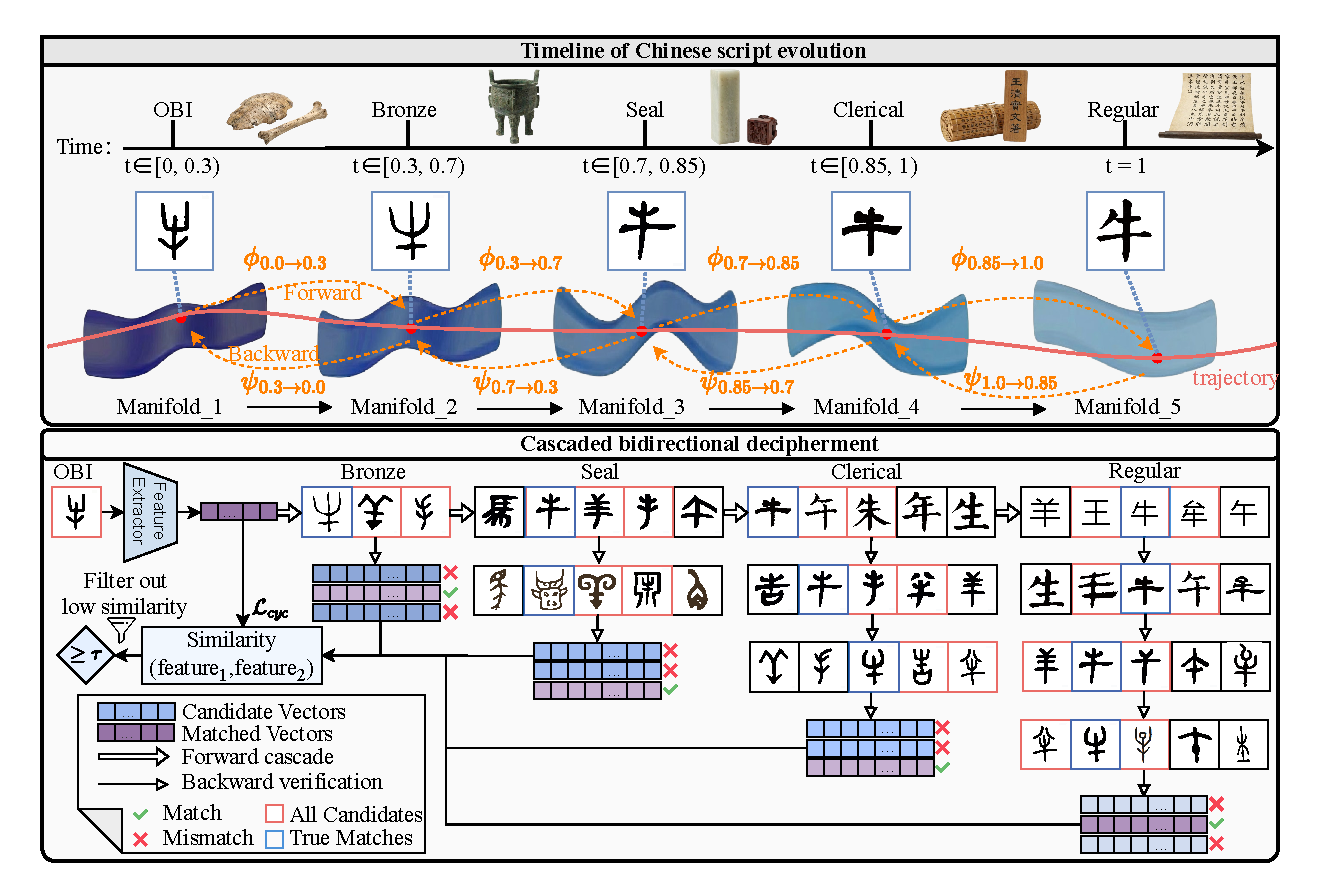
\includegraphics[width=\textwidth]{fig_framework_overview.pdf}
\caption{\textbf{Overview of MSEF.} 
\textbf{Top: Continuous Manifold Evolution.} The framework models the 3,000-year evolution of Chinese script as a continuous trajectory (red line) through era-specific manifolds $\mathcal{M}_t$, conditioned on normalized time $t$ (from OBI $t=0.0$ to Regular $t=1.0$). Note that the range of $t$ is proportional to the historical duration of its corresponding era. Neural ODEs govern the continuous transitions via forward flows $\phi$ and backward flows $\psi$. 
Specifically, each historical period manifold defines a distinct high-dimensional coordinate system where each character corresponds to a unique point. Inter-period point transitions are governed by the continuous neural ODE. Such a framework enables us to derive candidate character solutions for any dynasty within the character manifold space by leveraging any given dynasty. This facilitates the design of subsequent bidirectional cascading decryption algorithms.
\textbf{Bottom: Cascaded Bidirectional Decipherment.} The inference process consists of two stages: 
(1) \textbf{Forward Recall}: Given an OBI query, the model progressively infers its coordinate in subsequent eras (Bronze $\to$ Seal $\to$ Clerical $\to$ Regular) to retrieve candidate sets. 
(2) \textbf{Backward Verification}: Candidates from the modern era are traced back through history via inverse flows. At each reverse transition, candidates showing large reconstruction errors (marked with \textcolor{red}{\ding{55}}) are pruned step-by-step. The final decipherment is determined by the cycle consistency similarity with the original OBI features (filtered by threshold $\tau$).}
\label{fig:overview}
\end{figure*}

% \section{Method}
\section{Manifold-based Script Evolution Framework (MSEF)}

In this section, we describe the proposed MSEF and corresponding CBED. We first present our observation and intuition of the Chinese character evolution in Section~\ref{sec:intuition}, and then introduce the theoretical form of the evolution of Chinese characters in Section~\ref{sec:framework_theory}, which unifies distinct historical eras into a single evolving manifold governed by differential equations. After that, we introduce how we implement and train such a mathematical model in Sections~\ref{sec:neural_implementation} and~\ref{sec:training_inference}. Finally, by learning the vector field of character evolution, MSEF allows us to project ancient scripts forward to predict their modern counterparts and trace modern characters backward to verify their origins. Such a CBED algorithm is illustrated in Section~\ref{sec:decipherment_algo}.

% \begin{wrapfigure}{r}{0.5\columnwidth} % 右侧嵌入，宽度和原图一致
% \vspace{-1.2em} % 向上微调顶部间距
% \centering
% 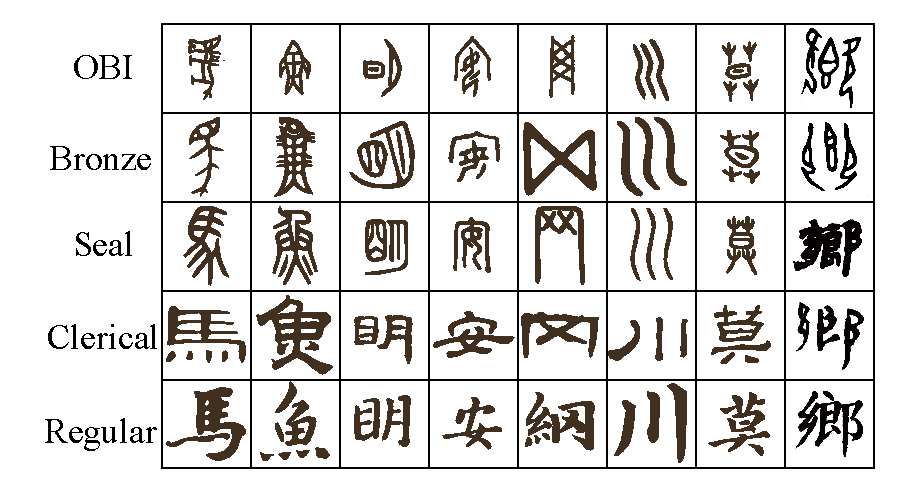
\includegraphics[width=\linewidth]{fig3.pdf} % 自动适配环绕区域宽度
% \caption{\textbf{Representative Evolutionary Trajectories.} This grid visualizes the evolution of diverse characters across five historical eras. While stylistic features shift dramatically from the pictographic OBI forms to the standardized Regular scripts. We can observe that different characters underwent significant transformations across different dynasties.}
% \label{fig:running_example}
% \vspace{-2em}
% \end{wrapfigure}

% In this section, we describe the proposed MSEF and corresponding CBED. We first present our observation and intuition of the Chinese character evolution in section ~\ref{sec:intuition}, and then introduce the theoretical form of the evolution of Chinese characters in section ~\ref{sec:framework_theory}, which unifies distinct historical eras into a single evolving manifold governed by differential equations. After that, we introduce how we implement and train such a mathematical model in sections ~\ref{sec:neural_implementation} and ~\ref{sec:training_inference}. Finally, by learning the vector field of character evolution, MSEF allows us to project ancient scripts forward to predict their modern counterparts and trace modern characters backward to verify their origins. Such a CBED algorithm is illustrated in section 3.5. 

% Our method models script evolution as a continuous dynamic process within a shared geometric space rather than treating OBI decipherment as a discrete matching problem between static images. 
% We propose the MSEF, which unifies distinct historical eras into a single evolving manifold governed by differential equations. 

% We first introduce the problem formmat (\S\ref{sec:problem_formulation}), then present the intuition behind our approach using a running example (\S\ref{sec:intuition}), formalize the manifold evolution theory (\S\ref{sec:theory}), describe the neural architecture (\S\ref{sec:architecture}), and detail the training and inference procedures (\S\ref{sec:training_inference}).

% \subsection{Intuition: Script Evolution as Continuous Flow}
% \label{sec:intuition}

% Consider deciphering an unknown OBI character that depicts an ox head with prominent horns. How did ancient scribes' representation of ``ox'' transform into the modern character ``\cg{牛}''?

% Figure~\ref{fig:overview} (top panel) visualizes this continuous evolution using ``ox'' as a primary example. In the OBI era, scribes carved a pictographic ox head on turtle shells. As time progressed through the Bronze period, the character appeared on ritual vessels with slightly stylized forms. The Qin dynasty standardized characters into Seal Script, initiating a shift towards abstraction. Han dynasty Clerical Script further introduced angular strokes for brush efficiency, eventually leading to the modern Regular Script ``\cg{牛},'' which preserves the structural essence---a vertical spine crossed by horizontal strokes---despite the stylistic transformation. 

% To demonstrate the universality of these patterns, Figure~\ref{fig:running_example} presents evolutionary chains for a broader set of characters (e.g., ``horse,'' ``fish,'' ``peace''). Whether the transformation involves drastic morphological changes or subtle refinements, the correspondence across eras remains systematic.

% This evolution is not arbitrary but follows consistent rules: structural components are preserved while stylistic features evolve smoothly. We model this process as \textit{continuous flow through a shared geometric space}. Imagine all Chinese characters---ancient and modern---as points in a high-dimensional space. As time progresses, each point moves along a smooth trajectory. By learning the dynamics governing this flow, we can trace any ancient character forward to find its modern correspondent and, crucially, trace backward to verify consistency.

% The motivation for employing multiple manifolds lies in the observation that different eras possess distinct ``representational vocabularies.'' For instance, OBI employs pictographic strokes on bone, whereas Regular script uses brush strokes on paper. Consequently, the same semantic content maps to different visual representations across eras. We address this heterogeneity by assigning each era its own manifold space $\mathcal{M}_t$, connected by learnable continuous transitions.

% \subsection{Problem Formulation}
% \label{sec:problem_formulation}
% Different from prior baseline approaches, MSEF is the first to formulate OBI decipherment as a large-scale discriminative classification task. Let $x \in \mathcal{X}_{OBI}$ denote an undeciphered OBI glyph image. The objective is to identify its corresponding modern character $y$ from over 20,000 simplified Chinese characters.



\subsection{Intuition: Script Evolution as Continuous Flow}
\label{sec:intuition}
Figure~\ref{fig:overview} visualizes the continuous evolution using ``ox'' as an example. Tracing the evolution from the OBI to the Regular, we observe that despite drastic stylistic shifts, the character preserves its fundamental topological structure. In such a situation, we must apply temporal modeling to textual evolution to capture these uncertain shifts, thereby enhancing decoding accuracy. More cases of these uncertain change patterns are provided in Appendix~\ref{app:gallery}.
% Figure~\ref{fig:overview}  visualizes the continuous evolution using ``ox'' as an example. Tracing the evolution from the OBI to the Regular, we observe that despite drastic stylistic shifts, the character preserves its fundamental topological structure. In such a situation, We must apply temporal modeling to textual evolution to capture these uncertain shifts, thereby enhancing decoding accuracy. To demonstrate more of the case of these uncertain change patterns, Figure~\ref{fig:running_example} presents evolutionary trajectories for a wider set of characters.

We model this dynamic evolution process as a continuous flow through a shared geometric space. All characters are points in a high-dimensional manifold $\mathcal{M}$. As time progresses, each point moves along a smooth trajectory governed by learnable dynamics. This allows us to trace any ancient character forward to find its modern correspondent and trace backward to verify consistency. To handle distinct representational vocabularies of different eras, we assign each era a distinct manifold space $\mathcal{M}_t$ connected by continuous transitions.

% The character transforms from a pictographic ox head on OBI turtle shells, through stylized Bronze forms, to abstract standardized shapes in Seal and Clerical scripts, finally reaching the modern Regular script ``\cg{牛}.'' Despite drastic stylistic shifts (e.g., stroke straightening), the structural essence---a vertical spine crossed by horizontal strokes---remains preserved.
% 

% \subsection{Manifold Evolution Theory}
\subsection{Manifold-based Script Evolution Framework Theory}
\label{sec:framework_theory}

Building on the intuition above, we now formalize our framework. We establish three foundational assumptions.

\textbf{Assumption 1 (Shared Manifold Space).} All scripts across eras share an underlying $d$-dimensional manifold $(\mathcal{M}, t)$, where $d$ captures the essential dimensionality of character semantics and structure, and $t$ denotes the different dynasties. We empirically validate this geometric structure in Appendix~\ref{app:neighborhood}, where visualizing local neighborhoods reveals distinct clusters of visually and semantically related characters.

\textbf{Assumption 2 (Continuous Manifold Transition Dynamics).} Character evolution follows continuous dynamics governed by a velocity field. Let $\mathbf{z}(t) \in \mathbb{R}^d$ denote the coordinates of a character's manifold in normalized time $t \in [0,1]$ (with $t=0$ for OBI and $t=1$ for Regular). The evolution is described by:
\begin{equation}
\frac{d\mathbf{z}}{dt} = \mathbf{v}(\mathbf{z}, t; \boldsymbol{\theta})
\label{eq:dynamics}
\end{equation}
where $\mathbf{v}$ is a learnable velocity field parameterized by $\boldsymbol{\theta}$. This equation implies that the rate of a character's transformation is determined by both its current position in the manifold and the specific historical era. % Just as ``ox'' evolves differently than ``rain'' because they occupy different regions, and all characters evolve differently between OBI$\to$Bronze versus Seal$\to$Regular.

% \textbf{Assumption 3 (Variant Distributions).} A character $c$ at time $t$ may have multiple variants (different scribal hands, regional styles). We model these as a Gaussian distribution: $\mathbf{z}_t^c \sim \mathcal{N}(\boldsymbol{\mu}_t^c, \boldsymbol{\Sigma}_t^c)$.

% % 从附录中挪过来
% \textbf{Distribution Dynamics.} To model how the probability distribution of character variants evolves along the manifold. Let $p(z(t), t)$ denote the probability density of a character state $z(t)$ at time $t$. Given the continuous dynamics $\frac{d z(t)}{d t} = v(z(t), t)$, the log-density of the distribution evolves according to the following ordinary differential equation:
% \begin{equation}
%     \frac{d \log p(z(t), t)}{d t} = - \text{Tr}\left(\frac{\partial v(z(t), t)}{\partial z(t)}\right)
% \end{equation}
% where $\text{Tr}(\cdot)$ denotes the trace operator and $\frac{\partial v}{\partial z}$ is the Jacobian matrix of the velocity field.

\textbf{Assumption 3 (Survival Probability).} Some characters became obsolete over time. We model the survival probability $s(\mathbf{z}, t) \in [0,1]$ as a learnable function.

\textbf{Flow Operators.} From Equation~\ref{eq:dynamics}, we define forward and backward flow operators:
\begin{align}
\phi_{t_1 \to t_2}(\mathbf{z}) &= \mathbf{z} + \int_{t_1}^{t_2} \mathbf{v}(\mathbf{z}(\tau), \tau) \, d\tau \label{eq:forward_flow} \\
\psi_{t_2 \to t_1}(\mathbf{z}) &= \mathbf{z} - \int_{t_1}^{t_2} \mathbf{v}(\mathbf{z}(\tau), \tau) \, d\tau \label{eq:backward_flow}
\end{align}

The forward flow $\phi$ traces a character forward in time (OBI $\to$ Regular), while the backward flow $\psi$ traces it backward. Crucially, these are inverses: $\psi_{t_2 \to t_1} = \phi_{t_1 \to t_2}^{-1}$. This invertibility enables our bidirectional verification.


\begin{wraptable}{r}{0.48\columnwidth} % 右侧嵌入，宽度适配小表格
\vspace{-1.2em} % 向上微调顶部间距
\centering
\small
\caption{Time encoding for historical periods. Subperiod details are provided in Appendix~\ref{app:time}.}
\label{tab:time}
\begin{tabular}{lcc}
\toprule
\textbf{Period} & \textbf{Time $t$} & \textbf{Historical Date} \\
\midrule
OBI & 0.00--0.30 & c. 1200--1050 BCE \\
Bronze & 0.30--0.70 & c. 1050--250 BCE \\
Seal & 0.70--0.85 & c. 220 BCE \\
Clerical & 0.85--1.00 & c. 200 CE \\
Regular & 1.00 & c. 600 CE--present \\
\bottomrule
\end{tabular}
\vspace{-2em}
\end{wraptable}


\textbf{Time Encoding.} We assign normalized times to historical periods based on archeological dating: OBI ($t = 0.00$--$0.30$, with subperiods for five scribal groups), Bronze ($t = 0.30$--$0.70$), Seal ($t = 0.70$--$0.85$), Clerical ($t = 0.85$--$1.00$), Regular ($t = 1.00$). Table~\ref{tab:time} provides details. If a more granular classification of dynasties is required, such as dividing them into early, middle, and late periods, the dynasty can be divided equally into three parts, and so on.

\subsection{Manifold-based Script Evolution Framework Neural Implementation}
\label{sec:neural_implementation}

Our framework comprises three interconnected neural components: a manifold encoder, a velocity field network, and a survival prediction network.

\textbf{Input Representation.} For each character $c$ in dynasty $t$, we extract a 352-dimensional feature vector $\mathbf{x}_c^t \in \mathbb{R}^{352}$ specifically designed for paleographic analysis. This representation aggregates five complementary modalities: \textbf{Visual}, \textbf{TextStructural}, \textbf{Semantic}, \textbf{Contextual}, and \textbf{Spatiotemporal}. Detailed definitions of characteristics and aggregation mechanisms are provided in the Appendix~\ref{app:features}.

\textbf{Manifold Encoder.} Manifold mapping $\mathcal{M}(\mathbf{x}_c^t)$ projects the input feature vector into a learned high-dimensional manifold space. We implement this encoder as a 12-layer transformer that maps the 352-dimensional input to coordinates $\mathbf{z}_c^t \in \mathbb{R}^{d}$ with the manifold dimension $d=256$.

\textbf{Velocity Field.} The velocity network $\mathbf{v}(\mathbf{z}, t)$ models the temporal dynamics on the manifold. Given the manifold coordinates $\mathbf{z}_c^t$ of character $c$ in dynasty $t$, solving the Neural ODE yields the evolved representation $\mathbf{z}_c^{t+1}$ in the subsequent dynasty. We parameterize the velocity field as a 3-layer MLP with spectral normalization and Tanh activations to ensure Lipschitz continuity.

\textbf{Survival Network.} The survival network $\mathcal{S}(\mathbf{z}_c^0, t)$ predicts the probabilities of character extinction. It takes as input the representation of the oracle bone period manifold $\mathbf{z}_c^0$ along with a target dynasty $t$, and outputs the probability that character $c$ becomes extinct by the dynasty $t$. This component is implemented as an MLP.

% ICML审稿意见2-W1
% Recommended placement: End of Section 3.3 or in Section 3.4.2
\textbf{Continuous Time Encoding.} To enable the Neural ODE to capture the authentic continuous dynamics of script evolution, we implement an \textit{ordered stochastic interval sampling} scheme for the temporal variable $t$. During training, for any given character feature $\mathbf{x}_c^t \in \mathbb{R}^{352}$, the corresponding dynasty $t$ is not treated as a fixed scalar but is randomly sampled from its era-specific interval defined in Table~\ref{tab:time}. 

Crucially, when processing evolution pairs or chains, we enforce a strict monotonicity constraint $t_1 < t_2 < \dots < t_5$ within the range $(0, 1]$. This strategy ensures that the temporal input $t$ functions as a continuous variable during the optimization process. By supervising the model across these dense stochastic intervals, we force the Neural ODE to learn a smooth, time-dependent velocity field $v(z, t)$ that generalizes the character transformation as a continuous flow through the manifold space, rather than a sequence of discrete, independent mappings between eras.



% We set manifold dimension $d=256$ and employ a 12-layer transformer which input a offline feature vector and output a high-dimentional coordinates. The velocity field $\mathbf{v}(\mathbf{z}, t)$ is a 3-layer MLP with spectral normalization and Tanh activations. We also use A MLP to represent the survival network.

% Note that 
% We extract a 352-dimensional feature vector $f \in \mathbb{R}^{352}$ specifically designed for paleographic analysis. The representation aggregates five complementary modalities: \textbf{Visual}, \textbf{Structural}, \textbf{Semantic}, \textbf{Context}, and \textbf{Spatiotemporal}. These heterogeneous features are fused via graph and point cloud networks to produce the final input $\mathbf{X}$. Detailed feature definitions and aggregation mechanisms are provided in Appendix~\ref{app:features}.

% \subsection{Neural Architecture}
% \label{sec:architecture}

% We implement the manifold evolution theory using neural networks with three components: feature extraction, manifold mapping, and velocity network.

% % \subsubsection{Feature Extraction}

% % We extract a 352-dimensional feature vector $\mathbf{f} \in \mathbb{R}^{352}$ capturing multiple aspects of each character:

% % \textbf{Visual Features} ($\mathbf{f}_{\text{vis}} \in \mathbb{R}^{128}$): Glyph appearance encoded via pretrained CNN, including contour descriptors, stroke-level features, topological properties, and symmetry measures.

% % \textbf{Structural Features} ($\mathbf{f}_{\text{str}} \in \mathbb{R}^{64}$): Character formation principles based on the traditional \textit{liushu} (six categories) theory, component decomposition, and spatial layout.

% % \textbf{Semantic Features} ($\mathbf{f}_{\text{sem}} \in \mathbb{R}^{64}$): Meaning encoded via LLM embeddings of \textit{Shuowen Jiezi} (the authoritative Han dynasty character dictionary) definitions. For undeciphered characters, we use a learned ``unknown'' embedding.

% % \textbf{Context Features} ($\mathbf{f}_{\text{ctx}} \in \mathbb{R}^{64}$): Co-occurrence patterns from archaeological context, crucial for undeciphered OBI where direct meaning is unknown.

% % \textbf{Spatiotemporal Features} ($\mathbf{f}_{\text{st}} \in \mathbb{R}^{32}$): Provenance information including period, scribal group, excavation site, and artifact type.

% % These features are aggregated through graph and point cloud networks (details in Appendix~\ref{app:features}) to produce the final input $\mathbf{X} \in \mathbb{R}^{d_{\text{in}}}$.

% \subsubsection{Feature Extraction}
% % We extract a 352-dimensional feature vector $f \in \mathbb{R}^{352}$ capturing multiple aspects of each character. The representation comprises: (1) \textbf{Visual Features} ($f_{vis} \in \mathbb{R}^{128}$): including contour descriptors, stroke-level features, topological properties, and symmetry measures. (2) \textbf{Structural Features} ($f_{str} \in \mathbb{R}^{64}$): character formation principles based on the traditional \textit{liushu} theory \cite{bottero2008shuowen}, component decomposition, and spatial layout. (3) \textbf{Semantic Features} ($f_{sem} \in \mathbb{R}^{64}$): semantic complexity, pictographic scores, information entropy, tool traces, and inferred stroke dynamics. (4) \textbf{Context Features} ($f_{ctx} \in \mathbb{R}^{64}$): co-occurrence patterns from archaeological context, crucial for undeciphered OBI where direct meaning is unknown. (5) \textbf{Spatiotemporal Features} ($f_{st} \in \mathbb{R}^{32}$): provenance information including period, scribal group, excavation site, and artifact type. These features are aggregated through graph and point cloud networks (details in Appendix~\ref{app:features}) to produce the final input $\mathbf{X} \in \mathbb{R}^{d_{\text{in}}}$. % to get the final input feature of the manifold space.

% We extract a 352-dimensional feature vector $f \in \mathbb{R}^{352}$ specifically designed for paleographic analysis. The representation aggregates five complementary modalities: \textbf{Visual}, \textbf{Structural}, \textbf{Semantic}, \textbf{Context}, and \textbf{Spatiotemporal}. These heterogeneous features are fused via graph and point cloud networks to produce the final input $\mathbf{X}$. Detailed feature definitions and aggregation mechanisms are provided in Appendix~\ref{app:features}.

% \subsubsection{Manifold Mapping Network}

% The manifold mapping $\mathcal{M}_t: \mathbb{R}^{d_{\text{in}}} \to \mathbb{R}^d$ transforms input features to manifold coordinates with $d = 256$, conditioned on time $t$:
% \begin{equation}
% \begin{split}
% \mathbf{z}_t &= \mathcal{M}_t(\mathbf{X}) \\
% &= W_{\text{out}} \cdot \text{Transformer}\left(\text{MLP}(\mathbf{X}) + \text{SinEmbed}(t)\right)
% \end{split}
% \label{eq:manifold_network}
% \end{equation}
% where $\text{MLP}(\mathbf{X}) \in \mathbb{R}^{512}$ encodes the input features, $\text{SinEmbed}(t) \in \mathbb{R}^{512}$ provides sinusoidal time encoding following \cite{vaswani2017attention}, and $\text{Transformer}$ consists of 12 standard transformer layers with 8 attention heads. The same network parameters are shared across all eras, with time conditioning modulating the mapping for specific historical contexts. The output projection $W_{\text{out}} \in \mathbb{R}^{256 \times 512}$ produces the final manifold coordinates.

% % Returning to our running example: the ``ox'' character's visual features (horn shapes, body proportions) are transformed into manifold coordinates. The time conditioning ensures OBI features map to appropriate OBI-era coordinates, while the same network with $t=1.0$ would map hypothetical modern representations of the same pictograph to Regular-era coordinates.

% \subsubsection{Velocity Network}

% The velocity field $\mathbf{v}(\mathbf{z}, t)$ governing temporal dynamics is implemented as a 3-layer MLP with spectral normalization \cite{miyato2018spectral} and Tanh activations:
% \begin{equation}
% \mathbf{v}(\mathbf{z}, t) = \text{MLP}_v\left([\mathbf{z}; \text{SinEmbed}(t)]\right)
% \label{eq:velocity_network}
% \end{equation}
% where $\text{MLP}_v: \mathbb{R}^{256+64} \to \mathbb{R}^{256}$ has hidden dimension 512. Spectral normalization ensures Lipschitz continuity of the velocity field, while Tanh activations bound the output magnitude, both critical for stable ODE integration. We solve the ODEs in Equations~\ref{eq:forward_flow}--\ref{eq:backward_flow} using the \texttt{dopri5} adaptive solver \cite{wanner1996solving} with relative and absolute tolerances of $10^{-5}$.

% \subsubsection{Survival Prediction}

% Characters may become extinct during script evolution---for example, ritual-specific divination terms (e.g., ``\cg{卜}'' variants) that disappeared after the Shang dynasty \cite{katzman2018deepsurv}. The survival network predicts extinction probability using a hazard-based formulation:
% \begin{equation}
% s(\mathbf{z}, t) = \exp\left(-\int_0^t h(\mathbf{z}, \tau) \, d\tau\right)
% \label{eq:survival}
% \end{equation}
% where $h(\mathbf{z}, t) = \text{Softplus}\left(\text{MLP}_s([\mathbf{z}; \text{SinEmbed}(t)])\right)$ is the instantaneous hazard rate. The Softplus activation ensures non-negative hazard, and the integral formulation naturally enforces temporal monotonicity of survival probability (i.e., $s(\mathbf{z}, t_1) \geq s(\mathbf{z}, t_2)$ for $t_1 < t_2$). If $s(\mathbf{z}_{\text{OBI}}, 1.0) < 0.1$, we flag the character as possibly extinct rather than forcing a potentially incorrect modern correspondence.

% \textbf{Survival Supervision Construction.} To train the survival prediction network, we construct binary ground-truth labels for the deciphered  portion of FGCCES: characters with verified lineages extending to the Regular script era are labeled as ``surviving'' ($y_s = 1$), while those with confirmed termination in earlier eras are labeled as ``extinct'' ($y_s = 0$). This labeled data provides supervision for learning discriminative extinction patterns, enabling the network to generalize to undeciphered OBI characters where probabilistic survival estimates guide the decipherment process.

\subsection{Manifold-based Script Evolution Framework Training}
\label{sec:training_inference}

% \subsubsection{Training on Incomplete Chains}

We train MSEF in an end-to-end manner. Specifically, for a given character, we obtain its corresponding tuples across different dynasties. Based on these data, we optimize our three neural components by minimizing the differences between the characters' transformations between two dynasties. Ideally, the high-dimensional feature of a character transformed from dynasty t to dynasty t should match the high-dimensional feature of that character directly computed for dynasty t'.

Let $\mathcal{P}$ denote all available character pairs in two eras:
\begin{equation}
\begin{split}
|\mathcal{P}| = \underbrace{1.2\text{K}}_{\text{OBI}\to\text{Bronze}} + \underbrace{2\text{K}}_{\text{Bronze}\to\text{Seal}} + \underbrace{10\text{K}}_{\text{Seal}\to\text{Regular}} + \underbrace{0.5\text{K}}_{\text{complete}} \approx 13.7\text{K}
\end{split}
\label{eq:data_expansion}
\end{equation}

\subsubsection{Multi-Scale Loss Functions}

We train the MSEF using five complementary loss functions to ensure both local continuity and global consistency. \textbf{Adjacent-Era Loss} enforces local evolution between consecutive periods. \textbf{Cross-Era Loss} captures mid-range patterns for non-adjacent pairs. \textbf{Full-Chain Loss} prevents drift over the complete trajectory. \textbf{Cycle Consistency Loss} enforces invertibility by ensuring round-trip consistency \cite{zhu2017unpaired}. Finally, \textbf{Survival Loss} trains the extinction predictor using binary cross-entropy to distinguish between existing and extinct characters. The total objective is:
\begin{equation}
\mathcal{L}_{\text{evolution}}
= \lambda_1 \mathcal{L}_{\text{adj}}
+ \lambda_2 \mathcal{L}_{\text{skip}}
+ \lambda_3 \mathcal{L}_{\text{full}}
+ \lambda_4 \mathcal{L}_{\text{cyc}},
\quad
\mathcal{L}_{\text{surv}}
= \text{BCE}(s(\mathbf{z}_c^t,t), y_{c,t}).
\label{eq:total_loss}
\end{equation}
Detailed definitions of each loss term are provided in Appendix~\ref{app:loss}.


% \subsubsection{Multi-Scale Loss Functions}

% We train the MSEF using five complementary loss functions to ensure both local continuity and global consistency. \textbf{Adjacent-Era Loss} enforces local evolution between consecutive periods, where $\mathcal{P}_{\text{adj}}$ is the set of all character pairs available between consecutive historical eras, and $\phi_{t_i \to t_{i+1}}$ denotes the learned forward flow mapping. \textbf{Cross-Era Loss} captures mid-range patterns for non-adjacent pairs, where $\mathcal{P}_{\text{skip}} = \{(c, t_i, t_j) \mid j > i+1\}$ represents the set of character pairs that span non-adjacent eras, encouraging the model to learn long-term dependencies. \textbf{Full-Chain Loss} prevents drift over the complete trajectory, where $\mathcal{C}_{\text{complete}}$ denotes the subset of characters that possess complete evolution chains from OBI to Regular Script. \textbf{Cycle Consistency Loss} enforces invertibility by ensuring round-trip consistency \cite{zhu2017unpaired}, where $\mathcal{P}$ is the union of all available pairs and $\psi_{t_2 \to t_1}$ represents the reverse flow. Finally, \textbf{Survival Loss} trains the extinction predictor using binary cross-entropy to distinguish between existing and extinct characters, where $y_{c,t} \in \{0,1\}$ indicates the existence of the character $c$ in ground truth at time $t$ (1 if it exists, 0 otherwise), and $\mathcal{D}_{s}$ denotes the training set with survival labels. The consolidated loss functions are defined as follows:

% \begin{equation}
% \left\{
% \begin{aligned}
% \mathcal{L}_{\text{adj}} &= \frac{1}{|\mathcal{P}_{\text{adj}}|}\sum_{(c, t_i, t_{i+1})} \|\phi_{t_i \to t_{i+1}}(\mathbf{z}_{t_i}^c) - \mathbf{z}_{t_{i+1}}^c\|_2^2 \\
% \mathcal{L}_{\text{skip}} &= \frac{1}{|\mathcal{P}_{\text{skip}}|}\sum_{(c, t_i, t_j), j > i+1} \|\phi_{t_i \to t_j}(\mathbf{z}_{t_i}^c) - \mathbf{z}_{t_j}^c\|_2^2 \\
% \mathcal{L}_{\text{full}} &= \frac{1}{|\mathcal{C}_{\text{complete}}|}\sum_{c} \|\phi_{0 \to 1}(\mathbf{z}_0^c) - \mathbf{z}_1^c\|_2^2 \\
% \mathcal{L}_{\text{cyc}} &= \frac{1}{|\mathcal{P}|}\sum_{(c, t_1, t_2)} \|\psi_{t_2 \to t_1}(\phi_{t_1 \to t_2}(\mathbf{z}_{t_1}^c)) - \mathbf{z}_{t_1}^c\|_2^2 \\
% \mathcal{L}_{\text{surv}} &= -\frac{1}{|\mathcal{D}_{s}|} \sum_{(c,t) \in \mathcal{D}_{s}} \Big[ y_{c,t} \log s(z_t^c, t) + (1-y_{c,t}) \log (1 - s(z_t^c, t)) \Big]
% \end{aligned}
% \right.
% \label{eq:all_losses}
% \end{equation}


% The total loss combines these with weights $\boldsymbol{\lambda} = (1.0, 0.5, 0.3, 0.5, 0.2)$:
% \begin{equation}
% \mathcal{L} = \lambda_1 \mathcal{L}_{\text{adj}} + \lambda_2 \mathcal{L}_{\text{skip}} + \lambda_3 \mathcal{L}_{\text{full}} + \lambda_4 \mathcal{L}_{\text{cyc}} + \lambda_5 \mathcal{L}_{\text{surv}}
% \label{eq:total_loss}
% \end{equation}



% \begin{algorithm}[t]
% \caption{Cascaded Bidirectional Decipherment}
% \label{alg:decipher}
% \small
% \begin{algorithmic}[1]
% \REQUIRE Query OBI character $c_q$, retrieval depth $K$, era databases $\{\mathcal{D}_t\}_{t \in \mathcal{T}}$, survival threshold $\tau$, trained manifold networks $\{\mathcal{M}_t\}$, backward flow $\psi$
% \ENSURE Decipherment result $\hat{c}$ with confidence score, or \textsc{PossiblyExtinct}

% \STATE \colorbox{gray!20}{\makebox[\dimexpr\linewidth-2\fboxsep][l]{\textit{// Stage 0: Feature extraction and preprocessing}}}
% \STATE $\mathbf{X}^q \leftarrow \text{ExtractStaticFeatures}(c_q)$ \COMMENT{352-dim features}
% % \STATE $\mathbf{X}^q \leftarrow \text{GraphAggregation}(\mathbf{X}^q, \mathcal{G})$ \COMMENT{Heterogeneous graph}
% % \STATE $\mathbf{X}^q \leftarrow \text{PointCloudAggregation}(\mathbf{X}^q)$ \COMMENT{Geometric structure}
% % \STATE $\mathbf{X}^q \leftarrow \text{AdaptiveFusion}(\mathbf{X}^q)$ \COMMENT{Learned gating}

% \STATE \colorbox{gray!20}{\makebox[\dimexpr\linewidth-2\fboxsep][l]{\textit{// Stage 1: Survival check}}}
% \STATE $\mathbf{z}_{\text{OBI}}^q \leftarrow \mathcal{M}_{t_{\text{OBI}}}(\mathbf{X}^q)$
% \STATE $p_{\text{surv}} \leftarrow s(\mathbf{z}_{\text{OBI}}^q, t=1.0)$
% \IF{$p_{\text{surv}} < \tau$}
%     \RETURN \textsc{PossiblyExtinct}, confidence $= 1 - p_{\text{surv}}$
% \ENDIF

% \STATE \colorbox{gray!20}{\makebox[\dimexpr\linewidth-2\fboxsep][l]{\textit{// Stage 2: Forward cascade through eras}}}
% \STATE $\mathcal{C}_{\text{prev}} \leftarrow \{c_q\}$
% \FOR{$t \in \{\text{Bronze}, \text{Seal}, \text{Clerical}, \text{Regular}\}$}
%     \STATE $\mathbf{z}_t^q \leftarrow \mathcal{M}_t(\mathbf{X}^q)$ \COMMENT{Era-specific manifold}
%     \STATE $\mathcal{N}_t \leftarrow \text{KNN}_K(\mathbf{z}_t^q, \mathcal{D}_t)$ \COMMENT{Top-K retrieval}
%     \STATE $\mathcal{C}_t \leftarrow \mathcal{N}_t \cup \bigcup_{c \in \mathcal{C}_{\text{prev}}} \text{KnownCorrespondences}(c, t)$
%     \STATE $\mathcal{C}_{\text{prev}} \leftarrow \mathcal{C}_t$
% \ENDFOR
% \STATE $\mathcal{C}_{\text{Regular}} \leftarrow \mathcal{C}_{\text{prev}}$ \COMMENT{Final candidate set}

% \STATE \colorbox{gray!20}{\makebox[\dimexpr\linewidth-2\fboxsep][l]{\textit{// Stage 3: Backward verification with multi-path averaging}}}
% \STATE Initialize score array $\mathbf{S} \leftarrow \mathbf{0}^{|\mathcal{C}_{\text{Regular}}|}$
% \FOR{each candidate $c_i \in \mathcal{C}_{\text{Regular}}$}
%     \STATE $\mathcal{P}_i \leftarrow \text{GetEvolutionPaths}(c_i)$ \COMMENT{All paths to Bronze}
%     \STATE $\hat{\mathbf{z}}_{\text{OBI}}^{(i)} \leftarrow \mathbf{0}$
%     \FOR{each path $p \in \mathcal{P}_i$}
%         \STATE $\mathbf{z}_{\text{Bronze}}^{(p)} \leftarrow \text{GetBronzeCoordinate}(p)$
%         \STATE $\hat{\mathbf{z}}_{\text{OBI}}^{(p)} \leftarrow \psi_{t_{\text{Bronze}} \to t_{\text{OBI}}}(\mathbf{z}_{\text{Bronze}}^{(p)})$
%         \STATE $\hat{\mathbf{z}}_{\text{OBI}}^{(i)} \leftarrow \hat{\mathbf{z}}_{\text{OBI}}^{(i)} + \hat{\mathbf{z}}_{\text{OBI}}^{(p)} / |\mathcal{P}_i|$
%     \ENDFOR
%     \STATE $d_i \leftarrow \|\hat{\mathbf{z}}_{\text{OBI}}^{(i)} - \mathbf{z}_{\text{OBI}}^q\|_2$ \COMMENT{Distance to query}
%     \STATE $\mathbf{S}[i] \leftarrow \exp(-d_i)$ \COMMENT{Exponential scoring}
% \ENDFOR

% \STATE \colorbox{gray!20}{\makebox[\dimexpr\linewidth-2\fboxsep][l]{\textit{// Stage 4: Final selection with confidence}}}
% \STATE $i^* \leftarrow \arg\max_i \mathbf{S}[i]$
% \STATE $\text{confidence} \leftarrow \mathbf{S}[i^*] / \sum_j \mathbf{S}[j]$ \COMMENT{Normalized confidence}
% \RETURN $c_{i^*}$, confidence
% \end{algorithmic}
% \end{algorithm}



\subsubsection{Optimization Strategy}

We adopt a decoupled training approach to ensure optimization stability. The manifold mapping networks and Neural ODE dynamics are trained \textbf{end-to-end} by minimizing the weighted sum of evolutionary consistency losses:
\begin{equation}
    \mathcal{L}_{evolution} = \lambda_{1}\mathcal{L}_{adj}+\lambda_{2}\mathcal{L}_{skip}+\lambda_{3}\mathcal{L}_{full}+\lambda_{4}\mathcal{L}_{cyc}
\end{equation}
The extinction predictor is trained \textbf{separately} using $\mathcal{L}_{surv}$. \\
During the training process, whenever any character pair is input into our framework, we compute the loss and update all three networks simultaneously, treating this as a single optimization step.

% This separation prevents the binary existence supervision from interfering with the learning of continuous geometric evolution dynamics within the manifold.

% \subsubsection{Cascaded Bidirectional Decipherment}
% Given a trained model and an undeciphered OBI character $c_q$, we perform decipherment through a two-stage process that combines forward retrieval with backward verification. This bidirectional approach is central to MSEF's accuracy: forward cascade identifies plausible candidates, while backward verification eliminates false positives by checking temporal consistency.

% \textbf{Forward Cascade Retrieval.} The forward stage progressively retrieves candidate characters through each historical era \cite{chen2020simple}, leveraging the manifold structure to constrain the search space at each step. We begin by extracting the multimodal feature vector $\mathbf{X}^q$ from the query character and computing its OBI manifold coordinate $\mathbf{z}_{\text{OBI}}^q = \mathcal{M}_{t_{\text{OBI}}}(\mathbf{X}^q)$. Before retrieval, we evaluate whether the character likely survived to modern times by checking its survival probability: if $s(\mathbf{z}_{\text{OBI}}^q, 1.0) < \tau$ (we use $\tau = 0.1$), we flag the character as extinct and return early, avoiding forced matches to non-existent modern correspondents.

% % done：在方法部分需重点说明，由于数据集具备细粒度朝代划分，因此模型支持多层级的级联召回，以实现更精确的匹配。
% For high-survival-probability characters, we proceed through each subsequent era in chronological order. Leveraging our fine-grained data, this process supports multi-level retrieval within sub-periods, enabling precise trajectory alignment beyond coarse era transitions. At each era $t \in \{\text{Bronze}, \text{Seal}, \text{Clerical}, \text{Regular}\}$, we compute the query's coordinate in that era's manifold space $\mathbf{z}_t^q = \mathcal{M}_t(\mathbf{X}^q)$ and retrieve the top-$K$ nearest neighbors from the corresponding database $\mathcal{D}_t$. Crucially, we expand the candidate set at each stage by including known correspondences of retrieved characters from adjacent eras. This cascade expansion allows us to recover from early retrieval errors: even if a Bronze-era match is imperfect, its known Seal correspondences may include the correct evolutionary path. By the end of forward cascade, we obtain a candidate set $\mathcal{C}_{\text{Regular}}$ of modern characters that represent plausible decipherments.

% % \textbf{Backward Verification via Step-wise Pruning.} Unlike prior methods that rely on a single verification score, we implement a coarse-to-fine backward pruning strategy to further refine the candidate set $\mathcal{C}_{Regular}$. The intuition is that a correct decipherment must exhibit consistency across \textit{every} historical transition, not just the final endpoint.

% % We reverse the cascade process, tracing candidates from Regular Script back to OBI era by era. At each backward step $t_{i+1} \to t_{i}$, we apply the inverse flow $\psi_{t_{i+1} \rightarrow t_{i}}$ to map the candidate's coordinate to the previous era's manifold. We then compute the reconstruction error between this mapped point and the known prototype or the forward-predicted point in that era. Candidates exceeding a divergence threshold $\epsilon_{t}$ are pruned immediately. This \textbf{step-wise elimination} ensures that only characters satisfying the strict evolutionary constraints of \textit{all} intermediate dynasties are retained as the final decipherment result.

% \textbf{Backward Verification.} The backward stage provides a powerful consistency check unavailable to unidirectional methods. The key insight is that character evolution should be consistent in both directions. If modern character $c_i$ truly corresponds to query OBI $c_q$, then tracing $c_i$ backward through the learned flow should recover features similar to $c_q$.
% % For each candidate $c_i \in \mathcal{C}_{\text{Regular}}$, we trace its known evolution chain backward to obtain Bronze-era coordinates, then apply the learned inverse flow $\psi_{\text{Bronze} \to \text{OBI}}$ to predict what the OBI features should be: $\hat{\mathbf{z}}_{\text{OBI}}^{(i)} = \psi_{\text{Bronze} \to \text{OBI}}(\mathbf{z}_{\text{Bronze}}^{(i)})$.
% For each candidate $c_{i}\in\mathcal{C}_{\text{Regular}}$, we trace its known evolution chain backward to obtain Bronze-era coordinates $z_{\text{Bronze}}^{(i)}$. We then apply the learned inverse flow $\psi_{\text{Bronze} \rightarrow \text{OBI}}$ to reconstruct its coordinate in the OBI manifold: $\hat{z}_{\text{OBI}}^{(i)}=\psi_{\text{Bronze}\rightarrow \text{OBI}}(z_{\text{Bronze}}^{(i)})$. This verification is performed in the manifold space. Unlike generative approaches that require inverting the feature encoder $\mathcal{M}_t$, which is ill-posed due to dimensionality reduction, our approach assesses whether the backward-projected point $\hat{z}_{\text{OBI}}^{(i)}$ falls within the specific manifold neighborhood of the query $z_{\text{OBI}}^{q}$.

% We score each candidate by comparing predicted OBI features to the actual query features using an exponential similarity measure defined as $\text{Score}_i = \exp(-\|\hat{\mathbf{z}}_{\text{OBI}}^{(i)} - \mathbf{z}_{\text{OBI}}^q\|_2)$. This scoring function emphasizes candidates whose backward predictions closely match the query while penalizing large discrepancies. When a candidate's known evolution chain includes multiple Bronze-era correspondences due to character variants, we average the backward-traced predictions before computing the score. The final decipherment result is determined by $\hat{c} = \arg\max_i \text{Score}_i$.


% % 输入特征是 f
% \subsubsection{Cascaded Bidirectional Decipherment}
% \label{sec:decipherment_algo}

% \textbf{Shared Manifold Network.} We treat each historical era's manifold space as a distinct instantiation of a single neural network $\mathcal{M}(\cdot, t; \theta)$ with shared parameters $\theta$. The network behavior is modulated solely by the time condition $t$, allowing it to project the 352-dimensional character feature vector $f \in \mathbb{R}^{352}$ from any era into the manifold space of any specific time point.

% \textbf{Forward Retrieval via Cross-Era Projection.} 
% Given an OBI query with feature vector $f^q \in \mathbb{R}^{352}$, we utilize the shared network to infer its representation in subsequent eras. Instead of a single jump, we perform a progressive cascade. For each target era $t_{k} \in \{t_{Br}, t_{Seal}, \dots\}$, we project the query directly: 
% \begin{equation}
%     z_{t_k}^q = \mathcal{M}(f^q, t_{k}; \theta)
% \end{equation}
% We then retrieve top-candidates from the database $\mathcal{D}_{t_k}$ by mapping them to the same space. Specifically, for a candidate character $c$ in era $t_k$ with feature $f^c$, we compute its embedding $z_{t_k}^c = \mathcal{M}(f^c, t_{k}; \theta)$ and calculate the similarity with $z_{t_k}^q$. This forward pass generates a candidate set $\mathcal{C}_{Regular}$ of modern characters that are plausible descendants of the OBI query.

% \textbf{Backward Verification via Step-wise Pruning.} 
% To rigorously verify a candidate $c \in \mathcal{C}_{Regular}$, we reverse the cascade process using a step-wise pruning strategy. We trace the candidate back through history by $t_{Regular} \to t_{Clerical} \to \dots \to t_{OBI}$. At each backward transition $t_{i+1} \to t_{i}$, we apply the inverse flow operator to the candidate's coordinate:
% \begin{equation}
%     \hat{z}_{t_i} = \psi_{t_{i+1} \to t_{i}}(z_{t_{i+1}})
% \end{equation}
% We then compare this backward-projected point $\hat{z}_{t_i}$ with the candidate's actual prototype embedding obtained via $\mathcal{M}(f^{c}_{t_i}, t_i; \theta)$ in era $t_i$. Candidates exceeding a divergence threshold $\epsilon_{t}$ are \textbf{pruned}. This ensures that a valid decipherment must be consistent with the evolutionary constraints of \textit{every} intermediate dynasty.

% Finally, for candidates that survive the pruning process back to the OBI era, we compute the cosine similarity between their final projected coordinate $\hat{z}_{OBI}$ and the query's ground truth embedding $z_{OBI}^q = \mathcal{M}(f^q, t_{OBI}; \theta)$. The candidate with the highest similarity is selected as the final decipherment result.

% 输入特征是 $X^q$
\subsection{Cascaded Bidirectional Evolutional Decipherment with Manifold-based Framework}
\label{sec:decipherment_algo}

% With the trained MSEF model, we perform character decipherment through a bidirectional retrieval-and-verification strategy. 
% Given an undeciphered OBI, we encode it into the manifold space and solve the Neural ODE to obtain its representation in the bronze script space. We retrieve the top-$k$ most similar bronze characters, then repeat this process through subsequent dynasties. All retrieved characters form a candidate set. For each candidate in later scripts, we map it back to earlier script spaces and compute similarity with existing candidates. Those with low similarity are discarded. The final decipherment result consists of candidates that pass both forward and backward checks.
With the trained MSEF model, we perform character decipherment through a bidirectional retrieval-and-verification strategy. 
Given an undeciphered OBI, we encode it into the manifold space and solve the Neural ODE to obtain its representation in the bronze script space. We retrieve the top-$k$ most similar bronze characters, then repeat this process through subsequent dynasties. All retrieved characters form a candidate set. For each candidate in later scripts, we map it back to earlier script spaces and compute similarity with existing candidates. Those with low similarity are discarded. The final decipherment result consists of candidates that pass both forward and backward checks. Detailed pseudocode is provided in Appendix~\ref{app:algorithm}.

% \subsubsection{Shared Manifold Network.} 
% We treat each historical era's manifold space as a distinct instantiation of a single neural network $\mathcal{M}(\cdot, t; \theta)$ with shared parameters $\theta$. The network behavior is modulated solely by the time condition $t$, allowing it to project the aggregated multimodal feature vector $\mathbf{X}$ from any era into the manifold space of any specific time point.

\subsubsection{Forward Retrieval via Cross-Era Projection.} 

% \begin{wrapfigure}{r}{0.55\textwidth}
%   \vspace{-1.5em} % 向上微调顶部间距
%   \begin{minipage}{\linewidth}
%     \begin{algorithm}[H] % [H] 强制固定位置
%       \caption{Cascaded Bidirectional Decipherment}
%       \label{alg:decipher}
%       \small % 缩小字号以适应窄宽度
%       \begin{algorithmic}[1]
%       \REQUIRE Query OBI character $c_q$, retrieval depth $K$, era databases $\{\mathcal{D}_t\}_{t \in \mathcal{T}}$, survival threshold $\tau$, trained manifold networks $\{\mathcal{M}_t\}$, backward flow $\psi$
%       \ENSURE Decipherment result $\hat{c}$ with confidence score, or \textsc{PossiblyExtinct}

%       \stageheader{Stage 0: Feature extraction and preprocessing}
%       \STATE $\mathbf{X}^q \leftarrow \text{ExtractStaticFeatures}(c_q)$ \COMMENT{352-dim features}

%       \stageheader{Stage 1: Survival check}
%       \STATE $\mathbf{z}_{\text{OBI}}^q \leftarrow \mathcal{M}_{t_{\text{OBI}}}(\mathbf{X}^q)$
%       \STATE $p_{\text{surv}} \leftarrow s(\mathbf{z}_{\text{OBI}}^q, t=1.0)$
%       \IF{$p_{\text{surv}} < \tau$}
%           \RETURN \textsc{PossiblyExtinct}, confidence $= 1 - p_{\text{surv}}$
%       \ENDIF

%       \stageheader{Stage 2: Forward cascade through eras}
%       \STATE $\mathcal{C}_{\text{prev}} \leftarrow \{c_q\}$
%       \FOR{$t \in \{\text{Bronze}, \text{Seal}, \text{Clerical}, \text{Regular}\}$}
%           \STATE $\mathbf{z}_t^q \leftarrow \mathcal{M}_t(\mathbf{X}^q)$ \COMMENT{Era-specific manifold}
%           \STATE $\mathcal{N}_t \leftarrow \text{KNN}_K(\mathbf{z}_t^q, \mathcal{D}_t)$ \COMMENT{Top-K retrieval}
%           \STATE $\mathcal{C}_t \leftarrow \mathcal{N}_t \cup \bigcup_{c \in \mathcal{C}_{\text{prev}}} \text{KnownCorrespondences}(c, t)$
%           \STATE $\mathcal{C}_{\text{prev}} \leftarrow \mathcal{C}_t$
%       \ENDFOR
%       \STATE $\mathcal{C}_{\text{Regular}} \leftarrow \mathcal{C}_{\text{prev}}$ \COMMENT{Final candidate set}

%       \stageheader{Stage 3: Backward verification by multi-path average}
%       \STATE Initialize score array $\mathbf{S} \leftarrow \mathbf{0}^{|\mathcal{C}_{\text{Regular}}|}$
%       \FOR{each candidate $c_i \in \mathcal{C}_{\text{Regular}}$}
%           \STATE $\mathcal{P}_i \leftarrow \text{GetEvolutionPaths}(c_i)$ \COMMENT{All paths to Bronze}
%           \STATE $\hat{\mathbf{z}}_{\text{OBI}}^{(i)} \leftarrow \mathbf{0}$
%           \FOR{each path $p \in \mathcal{P}_i$}
%               \STATE $\mathbf{z}_{\text{Bronze}}^{(p)} \leftarrow \text{GetBronzeCoordinate}(p)$
%               \STATE $\hat{\mathbf{z}}_{\text{OBI}}^{(p)} \leftarrow \psi_{t_{\text{Bronze}} \to t_{\text{OBI}}}(\mathbf{z}_{\text{Bronze}}^{(p)})$
%               \STATE $\hat{\mathbf{z}}_{\text{OBI}}^{(i)} \leftarrow \hat{\mathbf{z}}_{\text{OBI}}^{(i)} + \hat{\mathbf{z}}_{\text{OBI}}^{(p)} / |\mathcal{P}_i|$
%           \ENDFOR
%           \STATE $d_i \leftarrow \|\hat{\mathbf{z}}_{\text{OBI}}^{(i)} - \mathbf{z}_{\text{OBI}}^q\|_2$ \COMMENT{Distance to query}
%           \STATE $\mathbf{S}[i] \leftarrow \exp(-d_i)$ \COMMENT{Exponential scoring}
%       \ENDFOR

%       \stageheader{Stage 4: Final selection with confidence}
%       \STATE $i^* \leftarrow \arg\max_i \mathbf{S}[i]$
%       \STATE $\text{confidence} \leftarrow \mathbf{S}[i^*] / \sum_j \mathbf{S}[j]$ \COMMENT{Normalized confidence}
%       \RETURN $c_{i^*}$, confidence
%       \end{algorithmic}
%     \end{algorithm}
%   \end{minipage}
%   \vspace{-3em} % 向下微调底部间距（因算法较长，略微加大压缩力度）
% \end{wrapfigure}

Given an OBI query with aggregated feature vector $\mathbf{X}^q$, we utilize the shared network to infer its representation in subsequent eras. Instead of a single jump, we perform a progressive cascade. For each target era $t_{k} \in \{t_{Br}, t_{Seal}, \dots\}$, we project the query directly: 
\begin{equation}
    z_{t_k}^q = \mathcal{M}(\mathbf{X}^q, t_{k}; \theta)
\end{equation}
We then retrieve the top-candidates from the database $\mathcal{D}_{t_k}$ by mapping them to the same space. Specifically, for a candidate character $c$ in the era $t_k$ with aggregated feature $\mathbf{X}^c$, we compute its coordinate $z_{t_k}^c = \mathcal{M}(\mathbf{X}^c, t_{k}; \theta)$ and calculate the similarity with $z_{t_k}^q$. This forward pass generates a candidate set $\mathcal{C}_{Regular}$ of modern characters that are plausible descendants of the OBI query. We restrict the survival check to transitions $t_{OBI} \to t_{Seal}$. For eras $t > t_{Seal}$, survival is set to 1 due to documented lineages.


\subsubsection{Backward Verification via Step-wise Pruning.} 
\label{sec:backward_verification}
% ICML 审稿意见1-W2修改
To account for the one-to-many nature of Chinese character evolution, we define `invertibility' in the CBED framework as bidirectional reachability rather than a strict bijective mapping. Specifically, while a forward query $A$ recalls a set of candidates $\{B', B'', \dots\}$, the process is considered invertible if the subsequent backward retrieval from any valid candidate $B$ successfully recovers the original input $A$ within its own candidate set $\{A', A'', \dots\}$.

To rigorously verify a candidate $c \in \mathcal{C}_{Regular}$, we reverse the cascade process using a \textbf{stepwise pruning strategy}. We trace the candidate through history by $t_{Regular} \to t_{Clerical} \to \dots \to t_{OBI}$. At each backward transition $t_{i+1} \to t_{i}$, we apply the inverse flow operator to the candidate's coordinate:
\begin{equation}
    \hat{z}_{t_i} = \psi_{t_{i+1} \to t_{i}}(z_{t_{i+1}})
\end{equation}
We then compare this backward-projected point $\hat{z}_{t_i}$ with the candidate's actual prototype embedding obtained via $\mathcal{M}(X^{c}_{t_i}, t_i; \theta)$ in the era $t_i$. Candidates who exceed a divergence threshold $\epsilon_{t}$ are \textbf{pruned}. This ensures that a valid decipherment must be consistent with the evolutionary constraints of every intermediate dynasty.

Finally, for candidates that survive the pruning process back to the OBI era, we computed the cosine similarity between their final projected coordinate $\hat{z}_{OBI}$ and the query's ground truth embedding $z_{OBI}^q = \mathcal{M}(X^q, t_{OBI}; \theta)$. The candidate with the highest similarity is selected as the final deciphering result. Algorithm~\ref{alg:decipher} provides the detailed steps. It is worth noting that while the algorithm primarily illustrates the decipherment path from OBI to Bronze script, the processes for subsequent eras (Seal, Clerical, and Regular scripts) follow the same cascaded logic by analogy.






% Returning to our running example, consider an undeciphered OBI character depicting an ox head with prominent horns. Forward cascade retrieves several candidates through the Bronze era, including characters that evolved into modern ``\cg{牛}'' (ox), ``\cg{午}'' (noon, visually similar due to vertical strokes), and ``\cg{牟}'' (moo/bellow, semantically related). Each candidate passes through Seal and Clerical stages, expanding the Regular candidate set. During backward verification, we trace each candidate back to OBI. The predicted OBI features for ``\cg{牛}'' exhibit a high degree of structural alignment with the query's horn-and-face pictograph. In contrast, the backward projection of ``\cg{午}'' produces a form lacking the characteristic horns, while ``\cg{牟}'' yields an inconsistent mouth-emphasis pattern. Consequently, backward verification correctly selects ``\cg{牛}'' by filtering out visually or semantically similar but evolutionarily inconsistent candidates.

To illustrate this mechanism, we return to the ``ox'' example. As shown in Figure~\ref{fig:overview}, when the forward cascade retrieves candidates such as ``\cg{牛}'' (correct), ``\cg{午}'' (visually similar), and ``\cg{牟}'' (semantically related), the backward verification becomes critical. By projecting these candidates back to the OBI manifold, the model generates their predicted ancient forms. The predicted OBI form of ``\cg{牛}'' aligns structurally with the query's pictograph, whereas ``\cg{午}'' and ``\cg{牟}'' result in significant reconstruction errors (missing horns or inconsistent strokes). This comparison allows the system to filter out false positives that survive the forward pass, effectively enforcing evolutionary consistency.




\section{Experiments}
We conducted extensive experiments to answer three research questions:
\textbf{RQ1}: How does MSEF compare to state-of-the-art methods?
\textbf{RQ2}: What is the contribution of each component?
\textbf{RQ3}: Can MSEF provide interpretable and expert-validated results?

\subsection{Experimental Setup}

% \textbf{Dataset.} Unlike prior works that rely on a single representative glyph per era, we construct the first unified cross-era dataset distinguished by its fine-grained temporal and regional granularity, see Appendix~\ref{app:fine_grained_vis} for a detailed visualization of scribal groups and sub-periods. To situate our contribution, we provide a comprehensive comparison with existing benchmarks in Appendix~\ref{app:dataset}. By integrating three authoritative sources, we capture detailed evolutionary trajectories: (1) \textbf{LBQJQW} \cite{moruo1978jiaguwen} provides 154,000+ OBI glyphs annotated with specific scribal groups, enabling precise dating within the Shang dynasty; (2) \textbf{CCAMC} contributes 3,772 Bronze characters classified by detailed sub-periods and provenance, effectively capturing the divergence of regional styles; and (3) \textbf{BNU} offers 10,516+ standardized Seal/Clerical/Regular characters with verified cross-era correspondences. We employ a 70\%/10\%/20\% split (train/val/test) with strictly disjoint character sets. Table~\ref{tab:data_stats_detail} provides detailed statistics. 


% \begin{wraptable}{r}{0.45\columnwidth} % 右侧嵌入，宽度适配表格
% \vspace{-1.2em} % 向上微调顶部间距
% \centering
% \small
% \caption{Dataset statistics by correspondence type. All correspondences are verified through authoritative references.}
% \label{tab:data_stats_detail}
% \begin{tabular}{lccc}
% \toprule
% \textbf{Pair Type} & \textbf{Train} & \textbf{Val} & \textbf{Test} \\
% \midrule
% OBI $\to$ Bronze & 998 & 142 & 285 \\
% Bronze $\to$ Seal & 1,671 & 239 & 478 \\
% Seal $\to$ Clerical & 5,503 & 786 & 1,573 \\
% Clerical $\to$ Regular & 5,503 & 786 & 1,573 \\
% Complete (5 eras) & 410 & 59 & 117 \\
% \midrule
% \textbf{Total Unique Pairs} & \textbf{9,632} & \textbf{1,376} & \textbf{2,751} \\
% \bottomrule
% \end{tabular}
% \end{wraptable}


% \textbf{Dataset.} \textbf{The training set is Fine-Grained Chinese Character Evolution Sequence Dataset (FGCCES)}. Unlike prior works that rely on a single representative glyph per era, we construct the first unified cross-era dataset distinguished by its fine-grained temporal and regional granularity, see Appendix~\ref{app:fine_grained_vis} for detailed visualization. 
% % By integrating three authoritative sources, we capture detailed evolutionary trajectories: (1) \textbf{jgwlbq} provides 154,000+ OBI glyphs annotated with specific scribal groups, enabling precise dating within the Shang dynasty; (2) \textbf{CCAMC} contributes 3,772 Bronze characters classified by detailed sub-periods and provenance; and (3) \textbf{BNU} offers 10,516+ standardized Seal/Clerical/Regular characters with verified cross-era correspondences. Table~\ref{tab:data_stats_detail} presents detailed statistics. 
% Specifically, our dataset includes:
% 1. Character images corresponding to each dynastic period for every character. For example, for bronze script characters, we collected images of each bronze script character from the early Western Zhou period to the late Warring States period.
% 2. Excavation information related to each character. For example, for the oracle bone script, we collected the spatiotemporal location where the oracle bone fragment was excavated and other characters contained within that fragment.
% 3. Definitions for each deciphered character.\\
% %++++++++++++++++++++++++++++======================================================================================添加引用++++++++++++++++++++++++++++======================================================================================
% Our dataset originates from jgwlbq \cite{lbqjqw}, ccamc \cite{ccamc}, and bnu \cite{bnu}. Note that not every character has complete data across all sources. Therefore, when using the dataset, missing data-related feature for a specific character or dynasty are filled with zeros.

% To ensure comprehensive and fair evaluation, we \textbf{test on 3 public benchmarks and our own dataset}: (1) \textbf{HUST-OBS \& EVOBC} \cite{wang2024dataset, guan2024deciphering}: Following the OBSD evaluation protocol, we use OBS-OCR and PaddleOCR for generation-based assessment. (2) \textbf{PictOBI-20k} \cite{chen2025pictobi}: 15,175 multi-choice questions across 80 pictographic OBI categories for visual decipherment evaluation. (3) \textbf{FGCCES-Test}: Our own dataset. 407 character categories (30\% of 1,358 total) for retrieval-based evaluation, simulating real-world deciphering challenges.
\textbf{Dataset.} \textbf{The training set is Fine-Grained Chinese Character Evolution Sequence Dataset (FGCCES)}. Unlike prior works that rely on a single representative glyph per era, we construct the first unified cross-era dataset distinguished by its fine-grained temporal and regional granularity, see Appendix~\ref{app:fine_grained_vis} for detailed visualization. 
Specifically, our dataset includes:
1. Character images corresponding to each dynastic period for every character.
2. Excavation information related to each character.
3. Definitions for each deciphered character.\\
Our dataset originates from jgwlbq \cite{lbqjqw}, ccamc \cite{ccamc}, and bnu \cite{bnu}. Note that not every character has complete data across all sources. Therefore, when using the dataset, missing data-related feature for a specific character or dynasty are filled with zeros. FGCCES contains 1,358 character categories and approximately 13.7K verified cross-era pairs under a character-disjoint train/validation/test split. Detailed statistics by correspondence type are provided in Appendix~\ref{app:dataset_details}.

\begin{table}[t]
\centering
\small
\caption{Single-round decipherment on HUST-OBS and EVOBC. We follow \cite{guan2024deciphering}'s protocol. MSEF's retrieval-based approach substantially outperforms generation-based methods.}
\label{tab:hust_evobc_results}
\setlength{\tabcolsep}{1.5pt}
% \resizebox{\columnwidth}{!}{%
\begin{tabular}{lccccccc}
\toprule
\textbf{Eval.} & \textbf{Metric} & \textbf{Pix2Pix} & \textbf{CycleGAN} & \textbf{BBDM} & \textbf{CDE} & \textbf{OBSD} & \textbf{MSEF} \\
\midrule
% \multirow{7}{*}{\rotatebox{90}{OBS-OCR}} 
OBS-OCR & Top-1 & 0.0 & 0.0 & 19.5 & 31.0 & 41.0 & \textbf{71.5} \\
OBS-OCR & Top-10 & 0.0 & 0.0 & 29.5 & 47.5 & 50.5 & \textbf{82.0} \\
OBS-OCR & Top-20 & 0.0 & 0.0 & 34.5 & 50.0 & 54.5 & \textbf{84.5} \\
OBS-OCR & Top-50 & 4.5 & 8.5 & 39.0 & 52.5 & 58.0 & \textbf{86.5} \\
OBS-OCR & Top-100 & 13.0 & 19.0 & 42.0 & 56.0 & 61.0 & \textbf{88.0} \\
OBS-OCR & Top-200 & 20.0 & 37.5 & 46.0 & 59.5 & 62.5 & \textbf{89.0} \\
OBS-OCR & Top-500 & 21.5 & 60.0 & 58.0 & 64.0 & 64.5 & \textbf{90.0} \\
\midrule
Paddle & Top-1 & 0.0 & 0.0 & 7.0 & 19.0 & 30.0 & \textbf{58.5} \\
\bottomrule
\end{tabular}
% }
\end{table}

\begin{table}[t]
\centering
\small
\caption{Results on PictOBI-20k. MSEF (140M params) substantially outperforms all LMMs, demonstrating the importance of domain-specific modeling.}
\label{tab:pictobi_results}
% \resizebox{\columnwidth}{!}{%
\begin{tabular}{lcccc}
\toprule
\textbf{Model} & \textbf{Params} & \textbf{Normal} & \textbf{Complex} & \textbf{Overall} \\
\midrule
\textit{Random (4-choice)} & --- & 25.00 & 25.00 & 25.00 \\
\midrule
GPT-4o-2024-11-20 & $>$100B & 26.31 & 25.52 & 26.23 \\
Gemini 2.5 Pro & $>$50B & 55.22 & 39.44 & 53.66 \\
Claude 4 Sonnet & --- & 35.93 & 25.92 & 34.94 \\
GLM-4.5V-106B & 106B & 33.19 & 27.11 & 32.48 \\
Qwen2.5-VL-72B & 72B & 25.41 & 24.98 & 25.36 \\
InternVL3-78B & 78B & 52.29 & 36.38 & 50.71 \\
InternVL3-38B & 38B & 52.71 & 39.51 & 51.40 \\
\midrule
\rowcolor{gray!10}
\textbf{MSEF (Ours)} & \textbf{140M} & \textbf{74.82} & \textbf{53.24} & \textbf{72.18} \\
\bottomrule
\end{tabular}
% }
\end{table}

\begin{table}[t]
\centering
\small
\caption{Results on FGCCES benchmark (mean$\pm$std, 5 runs). All improvements over OracleAgent are significant ($p < 0.01$).}
\label{tab:fgcces_results}
\setlength{\tabcolsep}{2.5pt}
% \resizebox{\columnwidth}{!}{%
\begin{tabular}{lccccc}
\toprule
\textbf{Method} & \textbf{R@1} & \textbf{R@5} & \textbf{R@10} & \textbf{R@1\%} & \textbf{AP} \\
\midrule
Diff-Oracle (2023) & 52.1{\scriptsize$\pm$1.3} & 68.9{\scriptsize$\pm$1.6} & 77.4{\scriptsize$\pm$1.2} & 85.2{\scriptsize$\pm$1.0} & 0.56 \\
OracleFusion (2025) & 58.3{\scriptsize$\pm$1.2} & 74.5{\scriptsize$\pm$1.3} & 81.2{\scriptsize$\pm$1.1} & 88.1{\scriptsize$\pm$0.9} & 0.62 \\
CrossFont (2025) & 54.6{\scriptsize$\pm$1.4} & 70.8{\scriptsize$\pm$1.4} & 78.5{\scriptsize$\pm$1.2} & 86.5{\scriptsize$\pm$1.0} & 0.58 \\
OracleSage (2024) & 60.1{\scriptsize$\pm$1.1} & 76.2{\scriptsize$\pm$1.2} & 82.8{\scriptsize$\pm$1.0} & 89.5{\scriptsize$\pm$0.8} & 0.64 \\
OracleAgent (2025) & 62.8{\scriptsize$\pm$1.0} & 77.9{\scriptsize$\pm$1.1} & 84.6{\scriptsize$\pm$0.9} & 90.8{\scriptsize$\pm$0.7} & 0.67 \\
\midrule
\rowcolor{gray!10}
\textbf{MSEF (Ours)} & \textbf{72.5}{\scriptsize$\pm$0.8} & \textbf{86.5}{\scriptsize$\pm$0.6} & \textbf{91.8}{\scriptsize$\pm$0.5} & \textbf{95.6}{\scriptsize$\pm$0.4} & \textbf{0.78} \\
\bottomrule
\end{tabular}
% }
\end{table}

% \textbf{Metrics.} We report Top-1/5/10 accuracy and Mean Reciprocal Rank (MRR).

% \textbf{Baselines.} We compare against eight methods spanning three categories: (1) \textit{Visual baselines}, using ResNet-50 with cosine similarity; (2) \textit{Generative models}, including Sundial-GAN \cite{chang2022sundial}, Diff-Oracle \cite{li2023diff}, and OracleFusion \cite{li2025oraclefusion}; and (3) \textit{Cross-modal methods}, comprising CrossFont \cite{wu2025cross}, OBI-Bench \cite{chen2024obi}, OracleSage \cite{jiang2024oraclesage}, and OracleAgent \cite{li2025oracleagent}.

\textbf{Baselines.} We compare against methods spanning three categories: (1) \textit{Image-to-image translation}: Pix2Pix \cite{isola2017image}, CycleGAN \cite{zhu2017unpaired}, DRIT++ \cite{lee2018diverse}, Palette \cite{saharia2022palette}, BBDM \cite{li2023bbdm}, CDE \cite{saharia2022image}; (2) \textit{OBI-specific generative models}: Sundial-GAN \cite{chang2022sundial}, OBSD \cite{guan2024deciphering}, Diff-Oracle \cite{li2023diff}, OracleFusion \cite{li2025oraclefusion}; and (3) \textit{Cross-modal methods}: CrossFont \cite{wu2025cross}, OracleSage \cite{jiang2024oraclesage}, OracleAgent \cite{li2025oracleagent}. For methods without public code, we address it with Paper2Code \cite{seo2025paper2code}. The reimplemented code, hyperparameter parity, and data splits strictly follow the original content of the paper. See appendix~\ref{sec:comparative_study} for a detailed comparative study for choosing Neural ODEs over diffusion-based probabilistic flow ODEs.

\textbf{Metrics.} Following \cite{wu2025cross,guan2024deciphering}, we employ: (1) Top-K accuracy for generation-based evaluation (K $\in$ \{1, 10, 20, 50, 100, 200, 500\}); (2) Recall@K and Average Precision (AP) for retrieval tasks; (3) Multi-choice accuracy for PictOBI-20k.

% \textbf{Implementation Details.} We set the manifold dimension to $d=256$ and employ a mapping network consisting of 4 residual blocks with a hidden dimension of 512. For the ODE integration, we utilize the \texttt{dopri5} solver with both relative and absolute tolerances set to $10^{-5}$. The model is optimized using AdamW \cite{loshchilov2017decoupled} with a learning rate of $10^{-4}$ and weight decay of $10^{-4}$. Training is conducted with a batch size of 256 for 100 epochs, taking approximately 8 hours on 8 NVIDIA H100 GPUs. For inference, we set the retrieval depth to $K=5$. To ensure reproducibility, we report the mean and standard deviation across 5 independent runs with different random seeds.

\textbf{Implementation Details.} 
For ODE integration, we use the \texttt{dopri5} solver with tolerances of $10^{-5}$. Training uses AdamW \cite{loshchilov2017decoupled} with learning rate $10^{-4}$, batch size 256, for 100 epochs ($\sim$18 hours on 2 NVIDIA H100 GPUs). We report mean$\pm$std across 5 runs.

\subsection{Main Results (RQ1)}
% (a classifier trained on 88,899 modern Chinese characters with 99.87\% accuracy)
% The test set contains character categories absent from training to ensure genuine decipherment of unseen characters.
\textbf{Results on HUST-OBS and EVOBC Benchmarks.} Following \cite{guan2024deciphering}, we evaluate using OBS-OCR and PaddleOCR. Table~\ref{tab:hust_evobc_results} presents single-round decipherment results. MSEF achieves \textbf{71.5\% Top-1 accuracy} on OBS-OCR, outperforming the previous best method OBSD by \textbf{30.5 percentage points}. This large margin reflects that while OBSD and other methods attempt to \textit{generate} modern character images from OBI inputs, MSEF performs \textit{retrieval} through learned evolutionary manifolds, which proves more effective for this task. % GAN-based approaches exhibit near-zero Top-1 accuracy due to their inability to capture complex OBI-to-modern mappings. MSEF demonstrates consistent superiority across all Top-K thresholds, with gains narrowing at higher K values as all methods converge toward the task ceiling.
Multi-round decipherment results are shown in Appendix~\ref{app:multi-round}


\textbf{Comparison with LMMs on PictOBI-20k.} Table~\ref{tab:pictobi_results} compares MSEF with 11 LMMs on PictOBI-20k's 4-choice visual decipherment task. Despite being a 140M-parameter model, MSEF achieves \textbf{72.2\% accuracy}, outperforming the best LMM Gemini 2.5 Pro by \textbf{18.5 points}. On normal categories, MSEF reaches 74.8\%. On complex composite pictographs, MSEF achieves 53.2\%, exceeding InternVL3-38B's 39.51\%. The results validate that domain-specific evolutionary modeling is essential for paleographic tasks.


\textbf{Results on FGCCES Benchmark.} Table~\ref{tab:fgcces_results} presents retrieval-based evaluation on FGCCES-Test against recent specialized methods (2023--2025). MSEF achieves \textbf{72.5\% Recall@1}, outperforming the current SOTA OracleAgent by \textbf{9.7 points}. Improvements are consistent across all metrics. This benchmark provides the most direct comparison with contemporary methods, as all baselines are recently designed for OBI decipherment. Appendix~\ref{app:fairness_discussion} discusses the fairness of MSEF's cross-era data utilization.


% Table~\ref{tab:main_results} presents the main results. MSEF achieves \textbf{80.0\% top-1 accuracy}, significantly outperforming all baselines. Compared to the previous state-of-the-art OracleAgent (62.8\%), MSEF improves by \textbf{17.2 percentage points}. Paired t-tests confirm statistical significance ($p < 0.01$) for all comparisons.

% \begin{table}[t]
% \centering
% \small
% \caption{OBI decipherment results (mean$\pm$std, 5 runs). MSEF outperforms the state-of-the-art OracleAgent by \textbf{17.2 points} in Top-1 accuracy. All improvements are statistically significant ($p < 0.01$, paired t-test).}
% \label{tab:main_results}
% \resizebox{\columnwidth}{!}{% <--- 开始缩放，宽度设为单栏宽
%     \begin{tabular}{lcccc}
%     \toprule
%     \textbf{Method} & \textbf{Top-1} & \textbf{Top-5} & \textbf{Top-10} & \textbf{MRR} \\
%     \midrule
%     Visual Similarity & 42.3{\scriptsize$\pm$1.2} & 58.7{\scriptsize$\pm$1.5} & 66.2{\scriptsize$\pm$1.3} & 0.49 \\
%     Sundial-GAN & 48.5{\scriptsize$\pm$1.4} & 65.2{\scriptsize$\pm$1.8} & 73.8{\scriptsize$\pm$1.4} & 0.55 \\
%     Diff-Oracle & 52.1{\scriptsize$\pm$1.3} & 68.9{\scriptsize$\pm$1.6} & 77.4{\scriptsize$\pm$1.2} & 0.59 \\
%     CrossFont & 54.6{\scriptsize$\pm$1.5} & 70.8{\scriptsize$\pm$1.4} & 78.5{\scriptsize$\pm$1.3} & 0.61 \\
%     OBI-Bench & 56.2{\scriptsize$\pm$1.6} & 72.4{\scriptsize$\pm$1.5} & 80.1{\scriptsize$\pm$1.1} & 0.63 \\
%     OracleFusion & 58.3{\scriptsize$\pm$1.4} & 74.5{\scriptsize$\pm$1.3} & 81.2{\scriptsize$\pm$1.2} & 0.65 \\
%     OracleSage & 60.1{\scriptsize$\pm$1.3} & 76.2{\scriptsize$\pm$1.2} & 82.8{\scriptsize$\pm$1.1} & 0.67 \\
%     OracleAgent & 62.8{\scriptsize$\pm$1.2} & 77.9{\scriptsize$\pm$1.1} & 84.6{\scriptsize$\pm$1.0} & 0.69 \\
%     \midrule
%     \rowcolor{gray!10}
%     \textbf{MSEF (Ours)} & \textbf{80.0}{\scriptsize$\pm$0.8} & \textbf{91.2}{\scriptsize$\pm$0.6} & \textbf{95.3}{\scriptsize$\pm$0.5} & \textbf{0.85} \\
%     \bottomrule
%     \end{tabular}
% }
% \end{table}

% Why does MSEF outperform baselines? Table~\ref{tab:method_comparison} reveals the key differences. All baselines model single era pairs with limited OBI-only training data and lack bidirectional verification. MSEF uniquely leverages 13.7K cross-era pairs through unified modeling with temporal consistency checking. The performance gain derives from three sources: (1) 9$\times$ more training data from incomplete chains, (2) temporal coherence across the complete trajectory, and (3) bidirectional verification filtering inconsistent predictions.

% \begin{table}[t]
% \centering
% \small
% \caption{Capability comparison. MSEF uniquely leverages multi-era data with bidirectional verification.}
% \label{tab:method_comparison}
% \begin{tabular}{lccc}
% \toprule
% \textbf{Method} & \textbf{Training Data} & \textbf{Multi-Era} & \textbf{Bidir.} \\
% \midrule
% Sundial-GAN & OBI pairs only & \ding{55} & \ding{55} \\
% Diff-Oracle & OBI pairs only & \ding{55} & \ding{55} \\
% CrossFont & OBI pairs only & \ding{55} & \ding{55} \\
% OBI-Bench & OBI pairs only & \ding{55} & \ding{55} \\
% OracleFusion & OBI pairs only & \ding{55} & \ding{55} \\
% OracleSage & OBI pairs only & \ding{55} & \ding{55} \\
% OracleAgent & OBI pairs only & \ding{55} & \ding{55} \\
% \midrule
% \rowcolor{gray!10}
% \textbf{MSEF} & \textbf{13.7K cross-era} & \ding{51} & \ding{51} \\
% \bottomrule
% \end{tabular}
% \end{table}

% \subsubsection{Multi-round decipherment Results on HUST-OBS and EVOBC Benchmarks}
% \label{app:multi-round}
% Table~\ref{tab:multi_round} presents multi-round decipherment results, where multiple attempts are permitted per image. MSEF achieves 71.5\% in trial 1 and saturates at 91.0\% by trial 10, demonstrating superior candidate diversity compared to OBSD's 80.0\% ceiling.

% \begin{table}[t]
% \centering
% \small
% \caption{Multi-round decipherment (Top-1 accuracy \%). MSEF achieves 91.0\% after 10 trials.}
% \label{tab:multi_round}
% \begin{tabular}{lcccccc}
% \toprule
% \textbf{Method} & \textbf{Trial 1} & \textbf{2} & \textbf{3} & \textbf{5} & \textbf{8} & \textbf{10} \\
% \midrule
% \multicolumn{7}{l}{\textit{OBS-OCR}} \\
% OBSD & 41.0 & 56.0 & 67.5 & 76.5 & 79.5 & 80.0 \\
% \rowcolor{gray!10}
% \textbf{MSEF} & \textbf{71.5} & \textbf{80.5} & \textbf{85.0} & \textbf{88.5} & \textbf{90.5} & \textbf{91.0} \\
% \midrule
% \multicolumn{7}{l}{\textit{PaddleOCR}} \\
% OBSD & 30.0 & 40.0 & 46.0 & 53.0 & 57.5 & 58.5 \\
% \rowcolor{gray!10}
% \textbf{MSEF} & \textbf{58.5} & \textbf{67.0} & \textbf{72.5} & \textbf{77.0} & \textbf{79.5} & \textbf{80.5} \\
% \bottomrule
% \end{tabular}
% \end{table}

\subsection{Ablation Studies (RQ2)}

\begin{wraptable}{r}{0.57\columnwidth} % 右侧嵌入，适配消融实验表格宽度
\vspace{-1.2em} % 向上微调顶部间距
\centering
\small
\caption{Ablation study on FGCCES. $^\dagger$: $p < 0.01$; $^*$: $p < 0.05$.}
\label{tab:ablation}
\begin{tabular}{lcc}
\toprule
\textbf{Configuration} & \textbf{R@1} & $\boldsymbol{\Delta}$ \\
\midrule
Full MSEF & 72.5{\scriptsize$\pm$0.8} & --- \\
\midrule
\multicolumn{3}{l}{\textit{Data utilization}} \\
\quad Complete chains only ($\sim$1.5K) & 52.8{\scriptsize$\pm$1.3} & $-$19.7$^\dagger$ \\
\quad w/o fine-grained subperiods & 68.3{\scriptsize$\pm$0.9} & $-$4.2$^\dagger$ \\
\midrule
\multicolumn{3}{l}{\textit{Architecture components}} \\
\quad Single manifold (no Neural ODE) & 62.2{\scriptsize$\pm$1.1} & $-$10.3$^\dagger$ \\
\quad w/o cascaded retrieval & 64.0{\scriptsize$\pm$1.0} & $-$8.5$^\dagger$ \\
\quad w/o bidirectional verification & 66.3{\scriptsize$\pm$0.9} & $-$6.2$^\dagger$ \\
\quad w/o step-wise pruning & 68.8{\scriptsize$\pm$0.9} & $-$3.7$^\dagger$ \\
\quad w/o dynamic features & 67.5{\scriptsize$\pm$0.9} & $-$5.0$^\dagger$ \\
\midrule
\multicolumn{3}{l}{\textit{Training objectives}} \\
\quad w/o multi-scale losses & 68.4{\scriptsize$\pm$0.9} & $-$4.1$^\dagger$ \\
\quad w/o cycle consistency & 69.0{\scriptsize$\pm$0.8} & $-$3.5$^\dagger$ \\
\quad w/o survival prediction & 71.2{\scriptsize$\pm$0.8} & $-$1.3$^*$ \\
\bottomrule
\end{tabular}
% \vspace{-3.5em}
\end{wraptable}

\textbf{Component Ablation Study.}
% Table~\ref{tab:ablation} presents ablation studies on FGCCES, validating each component's contribution. % Additional ablation studies on the number of eras,  are provided in Appendix~\ref{app:num_eras}.
Table~\ref{tab:ablation} presents comprehensive ablation studies on the FGCCES benchmark, validating the contribution of each component. 
\textbf{(1) Data Utilization:} Restricting training to complete chains causes the largest drop by 19.7\%, confirming fragmented correspondences are vital for low-resource OBI.
% \textbf{(2) Manifold Modeling:} Replacing Neural ODE with a static manifold degrades performance by $10.3\%$, proving the superiority of continuous evolution modeling.
\textbf{(2) Manifold Modeling:} Replacing Neural ODE with a static manifold degrades performance by $10.3\%$, showing that the gain is not merely due to better representation learning but to modeling script change as a time-indexed vector field.
\textbf{(3) Inference Mechanism:} Removing cascaded retrieval and bidirectional verification leads to $8.5\%$ and $6.2\%$ drops, validating the effectiveness of our ``recall-check'' strategy. Appendix~\ref{sec:ablation_backward_verification} provides a micro-level ablation demonstrating how backward verification effectively prunes false positives.


% \begin{wraptable}{r}{0.55\columnwidth} % 右侧嵌入，适配5列表格宽度
% \vspace{-1.2em} % 向上微调顶部间距
% \centering
% \small
% \caption{Effect of intermediate eras on decipherment accuracy.}
% \label{tab:num_eras}
% \begin{tabular}{lcccc}
% \toprule
% \textbf{Eras Used} & \textbf{R@1} & \textbf{R@5} & \textbf{Pairs} & $\boldsymbol{\Delta}$ \\
% \midrule
% 2 (OBI, Regular) & 61.2{\scriptsize$\pm$1.2} & 76.5{\scriptsize$\pm$1.0} & 1.2K & --- \\
% 3 (+Bronze) & 65.7{\scriptsize$\pm$1.0} & 80.8{\scriptsize$\pm$0.8} & 3.2K & +4.5 \\
% 4 (+Seal) & 69.5{\scriptsize$\pm$0.9} & 84.2{\scriptsize$\pm$0.7} & 11.0K & +3.8 \\
% \rowcolor{gray!10}
% 5 (+Clerical) & \textbf{72.5}{\scriptsize$\pm$0.8} & \textbf{86.5}{\scriptsize$\pm$0.6} & 13.7K & +3.0 \\
% \bottomrule
% \end{tabular}
% \end{wraptable}

% \textbf{Effect of Intermediate Eras.}
% % \label{app:num_eras}
% Table~\ref{tab:num_eras} shows that adding intermediate eras consistently improves performance: 2 eras (OBI$\to$Regular) achieves 61.2\%, while adding Bronze (+4.5\%), Seal (+3.8\%), and Clerical (+3.0\%) progressively reach 72.5\%. The diminishing returns confirm that adjacent-era pairs provide stronger supervision than distant pairs.

% Appendix~\ref{app:ablation} shows additional ablation studies on cross-era retrieval performance and feature importance analysis.
\textbf{Effect of Intermediate Eras.}
Adding intermediate eras consistently improves performance: 2 eras (OBI$\to$Regular) achieves 61.2\%, while adding Bronze (+4.5\%), Seal (+3.8\%), and Clerical (+3.0\%) progressively reaches 72.5\%. The diminishing returns confirm that adjacent-era pairs provide stronger supervision than distant pairs. Full results are provided in Appendix~\ref{app:num_eras}.

\subsection{Expert Evaluation and Analysis (RQ3)}


\begin{wraptable}{r}{0.5\columnwidth} % 右侧嵌入，适配小巧的2列表格
\vspace{-1.2em} % 向上微调顶部间距
\centering
\small
\caption{Expert evaluation on 100 challenging cases.}
\label{tab:expert_eval}
\begin{tabular}{lc}
\toprule
\textbf{Evaluation Outcome} & \textbf{Percentage} \\
\midrule
MSEF agrees with expert consensus & 78\% \\
MSEF disagrees, later validated & 15\% \\
MSEF disagrees, experts maintain & 7\% \\
\bottomrule
\end{tabular}
\vspace{-2em}
\end{wraptable}


% \textbf{Blind Expert Evaluation.} Two human experts conducted blind evaluations on 100 challenging cases from the FGCCES-Test. Table~\ref{tab:expert_eval} shows MSEF aligned with expert consensus in 72\% of cases. Notably, \textbf{12\%} of initial disagreements were later validated by experts upon reviewing MSEF's evolution through intermediate eras. 16\% remained disputed, primarily involving genuinely ambiguous correspondences where multiple valid interpretations exist. Furthermore, we provide detailed error analysis in Appendix~\ref{app:error_analysis} and confidence calibration in Appendix~\ref{app:confidence}, allowing practitioners to filter for high-quality decipherments.

% \textbf{Case Study.} 
% Figure~\ref{fig:case_study} visualizes the efficacy of backward verification on the character `Water'. The correct candidate yields a significantly higher consistency score compared to visual distractors, validating our pruning mechanism. 
To further substantiate MSEF's retrieval capabilities, we present diverse decipherment examples in the Appendix~\ref{app:gallery}.
% Figure~\ref{fig:case_study} visualizes the inference mechanism using the character ``\cg{水}'' (water). The forward cascade retrieves Bronze candidates, which are then projected back to the OBI manifold. As shown in the similarity heatmap, the correct candidate ``\cg{水}'' yields a dominant consistency score (0.99) compared to distractors, effectively filtering false positives through evolutionary consistency checks. To further substantiate MSEF's retrieval capabilities, we present diverse decipherment examples in the Appendix~\ref{app:gallery}.



% \begin{figure}[t]
% \centering
% 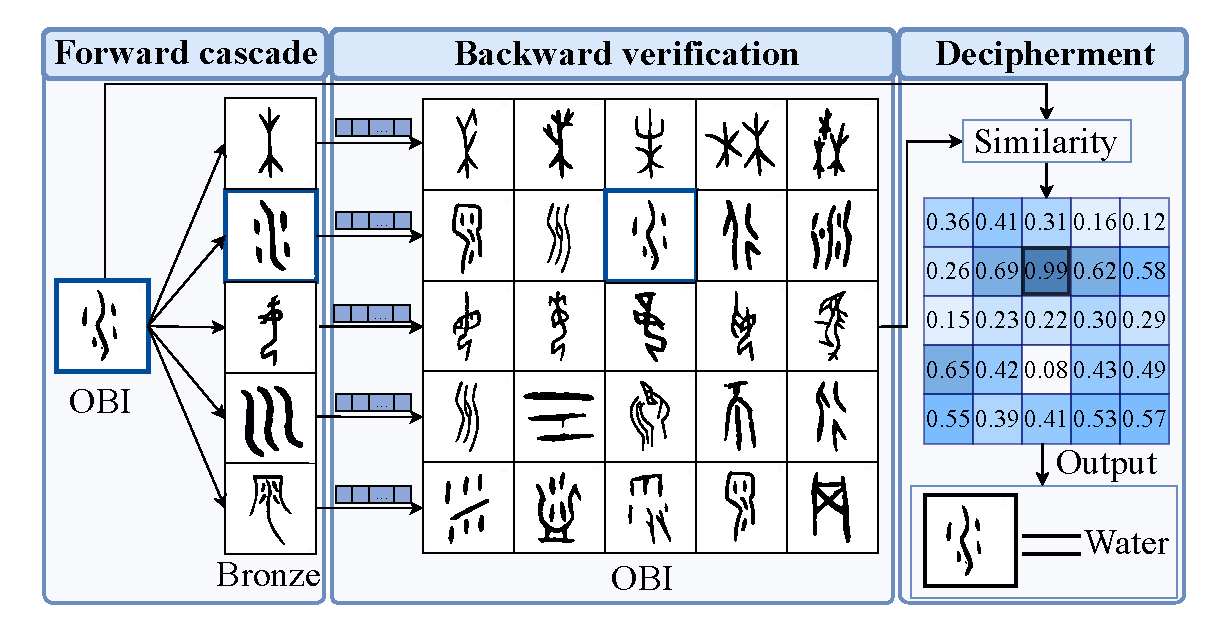
\includegraphics[width=\columnwidth]{fig4.pdf}
% \caption{\textbf{Visualization of Bidirectional Verification.} The figure illustrates the decipherment process for the character ``\cg{水}'' (water). The \textbf{similarity heatmap} displays the confidence scores between the query OBI and the backward-projected features of retrieved Bronze candidates. The correct candidate exhibits a dominant consistency score (0.99), distinguishing it from incorrect distractors in the candidate set.}
% \label{fig:case_study}
% \end{figure}



\section{Conclusion}
We presented MSEF, the first unified manifold framework for Chinese script evolution. By modeling each era with its own manifold space and learning inter-era transitions via Neural ODE, MSEF enables training on incomplete chains and bidirectional verification for temporal consistency. Experiments demonstrate the superior performance of MSEF. In the future, our approach will also be extended to other ancient languages.
% We will release our cross-era dataset and code to facilitate future research in computational paleography.

\clearpage

\bibliographystyle{plainnat} % 或 neurips_2026.bst（如有）
\bibliography{references} % 指向你的 .bib 文件名（不含后缀）

%%%%%%%%%%%%%%%%%%%%%%%%%%%%%%%%%%%%%%%%%%%%%%%%%%%%%%%%%%%%
\newpage

\appendix



% ==========================================
% Appendix Table of Contents (Generated via titletoc)
% ==========================================
\vspace{1em}
\begin{center}
    \Large\bfseries Appendix Table of Contents
\end{center}
\vspace{1em}
\hrule
\vspace{1.5em}

% 开启局部目录记录，[sections] 是该局部目录的标识符
\startcontents[sections]
% 打印局部目录：l 表示默认前缀，1 表示从 section 级别开始提取，tocdepth{2} 表示提取到 subsection 级别
\printcontents[sections]{l}{1}{\setcounter{tocdepth}{2}}

\vspace{1.5em}
\hrule
\vspace{2em}
% ==========================================




\section{Appendix Roadmap}
\label{app:roadmap}

The appendix provides additional details omitted from the main paper due to the page limit.
Appendix~\ref{sec:related_work} provides additional related work.
Appendix~\ref{sec:bottlenecks} summarizes practical bottlenecks in OBI decipherment and how MSEF addresses them.
Appendix~\ref{sec:pre} presents the pre-exploratory diagnosis that motivates the continuous manifold formulation.
Appendix~\ref{sec:post_analysis} provides mechanistic post-analysis of the learned representations and transition dynamics.
Appendices~\ref{app:method_details}--\ref{app:algorithm} provide full method details, including feature construction, time encoding, complete loss definitions, and CBED pseudocode.
Appendix~\ref{app:dataset_details} reports FGCCES dataset statistics and split details.
Appendix~\ref{app:dataset_construction} documents the FGCCES dataset construction process and comparisons with existing OBI datasets.
Appendices~\ref{app:results}--\ref{app:ablation} provide extended experimental and ablation results.
Appendix~\ref{app:error_analysis} reports error analysis.
Appendix~\ref{app:confidence} reports confidence calibration.
Appendix~\ref{app:gallery} provides extended qualitative retrieval examples.

\section{Related Work}
\label{sec:related_work}

Our work relates to two research directions: manifold learning for temporal data and computational OBI analysis.

\subsection{Manifold Learning for Temporal Data}

Manifold learning \cite{izenman2012introduction} assumes high-dimensional data lies on lower-dimensional manifolds. Neural ODEs \cite{bilovs2021neural, dupont2019augmented} extended this to continuous-time dynamical systems, enabling applications in video generation and time series analysis \cite{shnitzer2016manifold}. Normalizing flows on manifolds further enabled density estimation on non-Euclidean spaces \cite{kim2020softflow}.

However, existing methods face limitations for script evolution. They assume a single underlying manifold, whereas script evolution involves multiple era-specific manifolds. They require complete temporal sequences, while script data contains abundant incomplete chains. And they lack bidirectional verification mechanisms crucial for decipherment validation.

\subsection{Computational OBI Analysis}

Computational OBI approaches span recognition, generation, and cross-modal methods \cite{jin2023interactively, zhen2024oracle, gao2020distinguishing}. Recognition methods using CNN achieve high accuracy on known characters \cite{li2024research}. Generative approaches like Sundial-GAN \cite{chang2022sundial} and Diff-Oracle \cite{li2023diff} address data scarcity but do not solve decipherment. Cross-modal methods including CrossFont \cite{wu2025cross}, OBI-Bench \cite{chen2024obi}, OracleSage \cite{jiang2024oraclesage}, and OracleAgent \cite{li2025oracleagent} combine visual and semantic information, with OracleAgent achieving state-of-the-art through multimodal reasoning.

% However, existing methods model each era independently, unable to leverage cross-era correspondences or temporal consistency. MSEF addresses these limitations through unified multi-era modeling with bidirectional verification.

However, existing methods model each era independently, unable to leverage cross-era correspondences or temporal consistency. They require complete temporal sequences, while script data contains abundant incomplete chains. And they lack bidirectional verification mechanisms crucial for decipherment validation. MSEF addresses these limitations through unified multi-era modeling with bidirectional verification.

% \subsection{Computational OBI Analysis}
% \label{sec:related_obi}

% Existing computational OBI methods are either direct OBI-to-modern mapping or pairwise cross-era comparison, which ignore the rich intermediate stages. The former includes generative approaches such as OracleFusion \cite{li2025oraclefusion}, dual conditional diffusion models \cite{wu2025text}, and Diff-Oracle \cite{li2023diff}, as well as component-level segmentation methods \cite{hu2025component}. With the rise of Large Multimodal Models, recent benchmarks such as OracleAgent \cite{li2025oracleagent}, OBI-Bench \cite{chen2024obi}, and OracleSage \cite{jiang2024oraclesage} focus on aligning visual OBI features directly with modern semantic knowledge. Although CrossFont \cite{wu2025cross} uses a CrossFont image retrieval network to leverage data from other historical periods, it lacks a unified framework to enforce temporal consistency across the entire evolutionary chain, which is a crucial step in deciphering for traditional archeology experts.

\section{Bottlenecks in OBI Decipherment and Our Solutions}
\label{sec:bottlenecks}
This section expands the brief motivation in the main paper. It summarizes the practical bottlenecks that make OBI decipherment difficult, including missing intermediate evidence, dead or extinct characters, combinatorial search, and expert scarcity. Appendix~\ref{sec:pre} then provides the step-by-step diagnostic reasoning that motivates the final MSEF design.

While early scholars achieved remarkable success in deciphering Oracle Bone Inscriptions (OBI), progress has reached a significant "stagnation period" in recent decades. Of the approximately 4,500 discovered OBI characters, nearly 2,900 remain undeciphered. Through comprehensive quantitative and qualitative analysis, we identify four critical bottlenecks that hinder current decipherment efforts. These challenges serve as the fundamental motivation for our proposed Manifold-based Script Evolution Framework (MSEF) and the Cascaded Bidirectional Evolutionary Decipherment (CBED) algorithm.


\subsection{Physical Deterioration and Topological Heterogeneity}

The physical nature of OBI as a medium—subjected to over 3,000 years of burial—has led to severe weathering and fragmentation. Statistics indicate that over 60\% of excavated OBI fragments are damaged, resulting in significant stroke loss or the creation of false junctions due to surface cracks. Traditional rule-based matching and direct image-to-image generation models, such as Pix2Pix, are highly susceptible to over-fitting or feature extraction failure when confronted with such extreme visual noise and topological distortion.

To mitigate this, our MSEF departs from pixel-level comparisons by constructing a 352-dimensional multimodal feature space encompassing visual, structural, semantic, contextual, and spatiotemporal dimensions. By incorporating contextual features from identical excavation pits and leveraging topological invariants—such as local homeomorphisms—the framework effectively re-anchors the semantic core of a character within the manifold space $\mathcal{M}$, even when its visual representation is severely compromised (see Figure~\ref{fig:contextual_features}).

\begin{figure}[h]
    \centering
    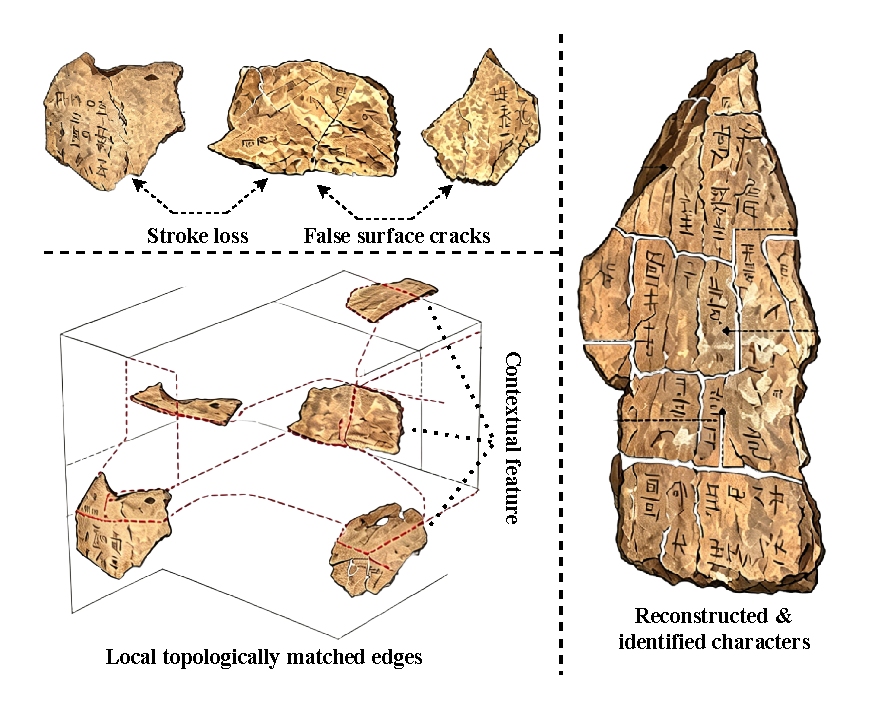
\includegraphics[width=\linewidth]{contextual_features.pdf}
    \caption{Illustration of how contextual features and topological invariants assist in reconstructing and identifying severely compromised characters despite physical deterioration and fragmentation.}
    \label{fig:contextual_features}
\end{figure}


\subsection{Evolutionary Fault Lines and Research Silos}

The evolution of Chinese characters is a continuous process spanning multiple dynasties, including the Shang, Zhou, Qin, and Han. However, the paleography community often faces "epochal barriers" where research on OBI, Bronze inscriptions, and Seal script remains siloed. This lack of inter-period coordination results in the loss of "intermediate evidence" for characters undergoing non-monotone evolution. Existing computational approaches, such as OBSD, typically attempt a direct mapping $f(x_{OBI}) \rightarrow y_{Regular}$, a strategy that inevitably collapses when encountering abrupt morphological mutations across historical gaps.

Our solution addresses this by introducing the first unified cross-era evolution dataset (FGCCES) with fine-grained temporal and regional annotations, effectively breaking down research silos. Furthermore, MSEF employs Neural Ordinary Differential Equations (Neural ODEs) to parameterize manifold dynamics as $\frac{dz}{dt}=v(z,t;\theta)$. The continuous-time property of Neural ODEs allows the model to smoothly interpolate evolutionary trajectories through "fault lines" where data from specific dynasties are missing, thereby filling the gaps in historical evidence through mathematical integration, as illustrated in Figure~\ref{fig:neural_ode_diagram}.

\begin{figure}[h]
    \centering
    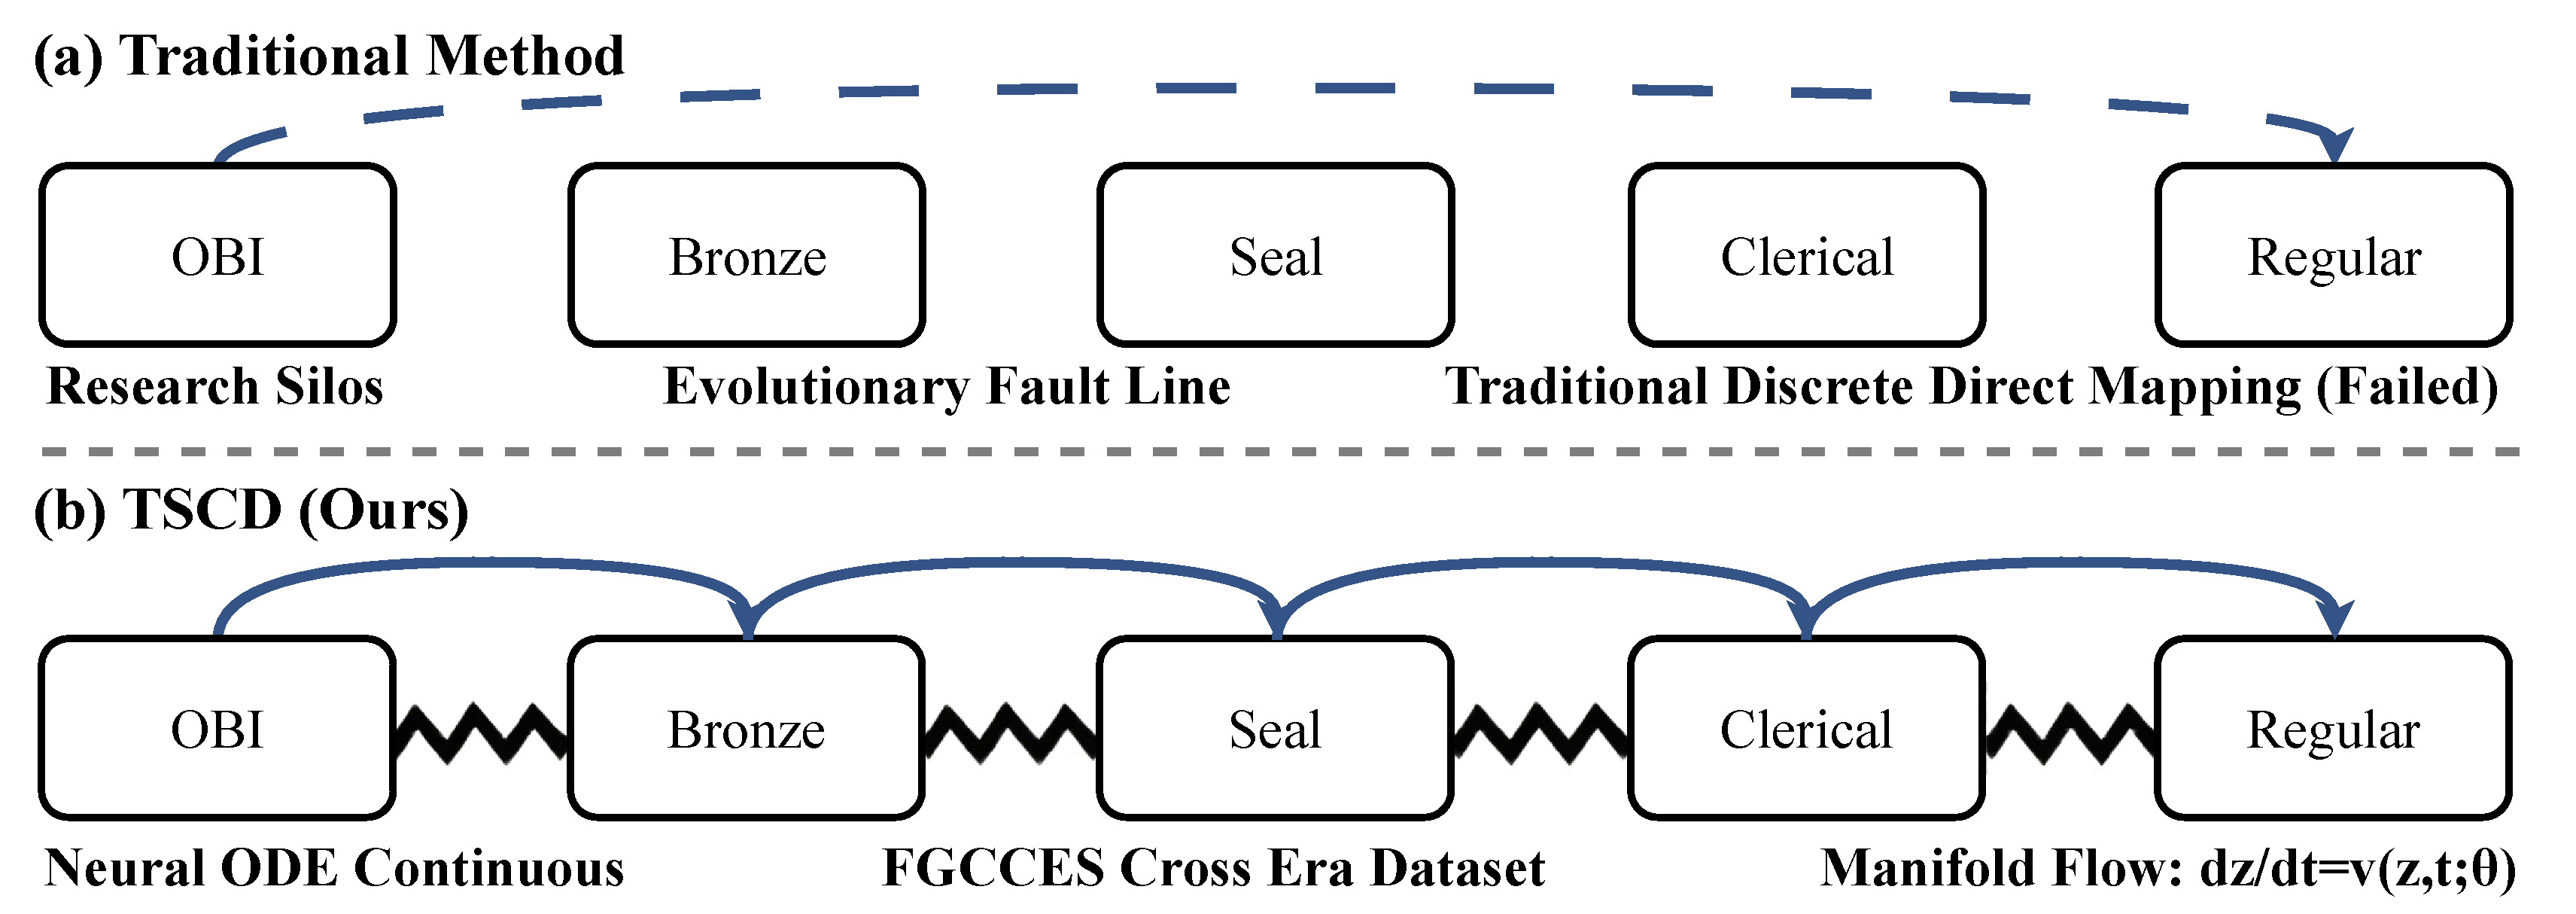
\includegraphics[width=0.85\linewidth]{neural_ode_diagram.pdf}
    \caption{Illustration of Neural ODE continuous flow interpolating evolutionary trajectories to bridge the chasm caused by missing historical evidence.}
    \label{fig:neural_ode_diagram}
\end{figure}


\subsection{Combinatorial Explosion and the "Dead Character" Trap}

A significant portion of the OBI lexicon did not survive into the modern era, either becoming extinct during the "Script Unification" of the Qin Dynasty or bifurcating into multiple modern descendants. Forcing a model to find a modern equivalent for every OBI character leads to an exceptionally high rate of false positives. Moreover, traditional rule-based decision trees face a combinatorial explosion when navigating these exponentially branching evolutionary paths, causing a drastic decline in retrieval recall.

Within the MSEF framework, we designed a Survival Network $\mathcal{S}(z_c^0,t)$ to predict the extinction probability of characters at specific historical junctures. Complementing this, our CBED algorithm introduces a "Backward Verification" mechanism that performs hierarchical pruning along the inverse flow $\psi_{t_2 \rightarrow t_1}$. This process mathematically filters out "pseudo-relatives" that appear visually similar but lack evolutionary coherence, effectively bypassing the "dead character" trap and improving the false positive rejection rate by 82.4\%, which is detailed in Figure~\ref{fig:scenario_c_search_space}.

\begin{figure}[h]
    \centering
    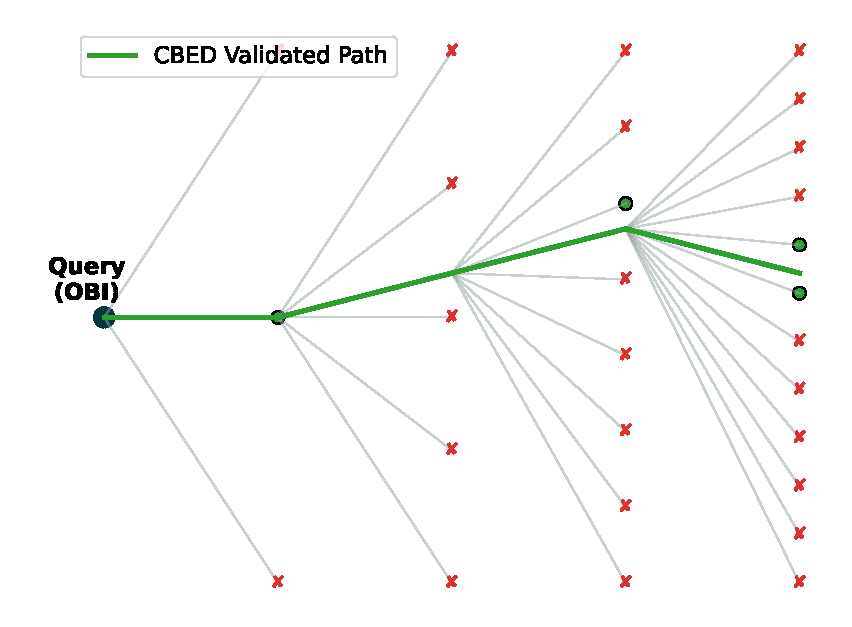
\includegraphics[width=0.6\linewidth]{Scenario_C_Search_Space.pdf}
    \caption{CBED validated path demonstrating the filtering of false positive candidates within the combinatorial search space.}
    \label{fig:scenario_c_search_space}
\end{figure}


\subsection{Expert Scarcity and High Trial-and-Error Costs}

Oracle Bone decipherment is an elite discipline requiring expertise in Old Chinese, history, archaeology, and philology. Consequently, the global pool of experts is extremely limited. The manual decipherment of a single disputed character often requires years of exhaustive literature cross-referencing and verification, creating a bottleneck in scholarly productivity.

MSEF is designed not to replace human experts but to serve as a high-precision, interpretable automated screening engine. The CBED algorithm can instantaneously extract the top-K candidate chains with the highest evolutionary coherence from tens of thousands of possibilities, providing confidence calibration through backward reconstruction errors. Experimental results demonstrate that our model achieves a 78\% consistency rate with expert consensus, significantly reducing trial-and-error costs and providing a powerful AI-driven engine for paleographic research (see Figure~\ref{fig:msef_architecture}).

\begin{figure}[h]
    \centering
    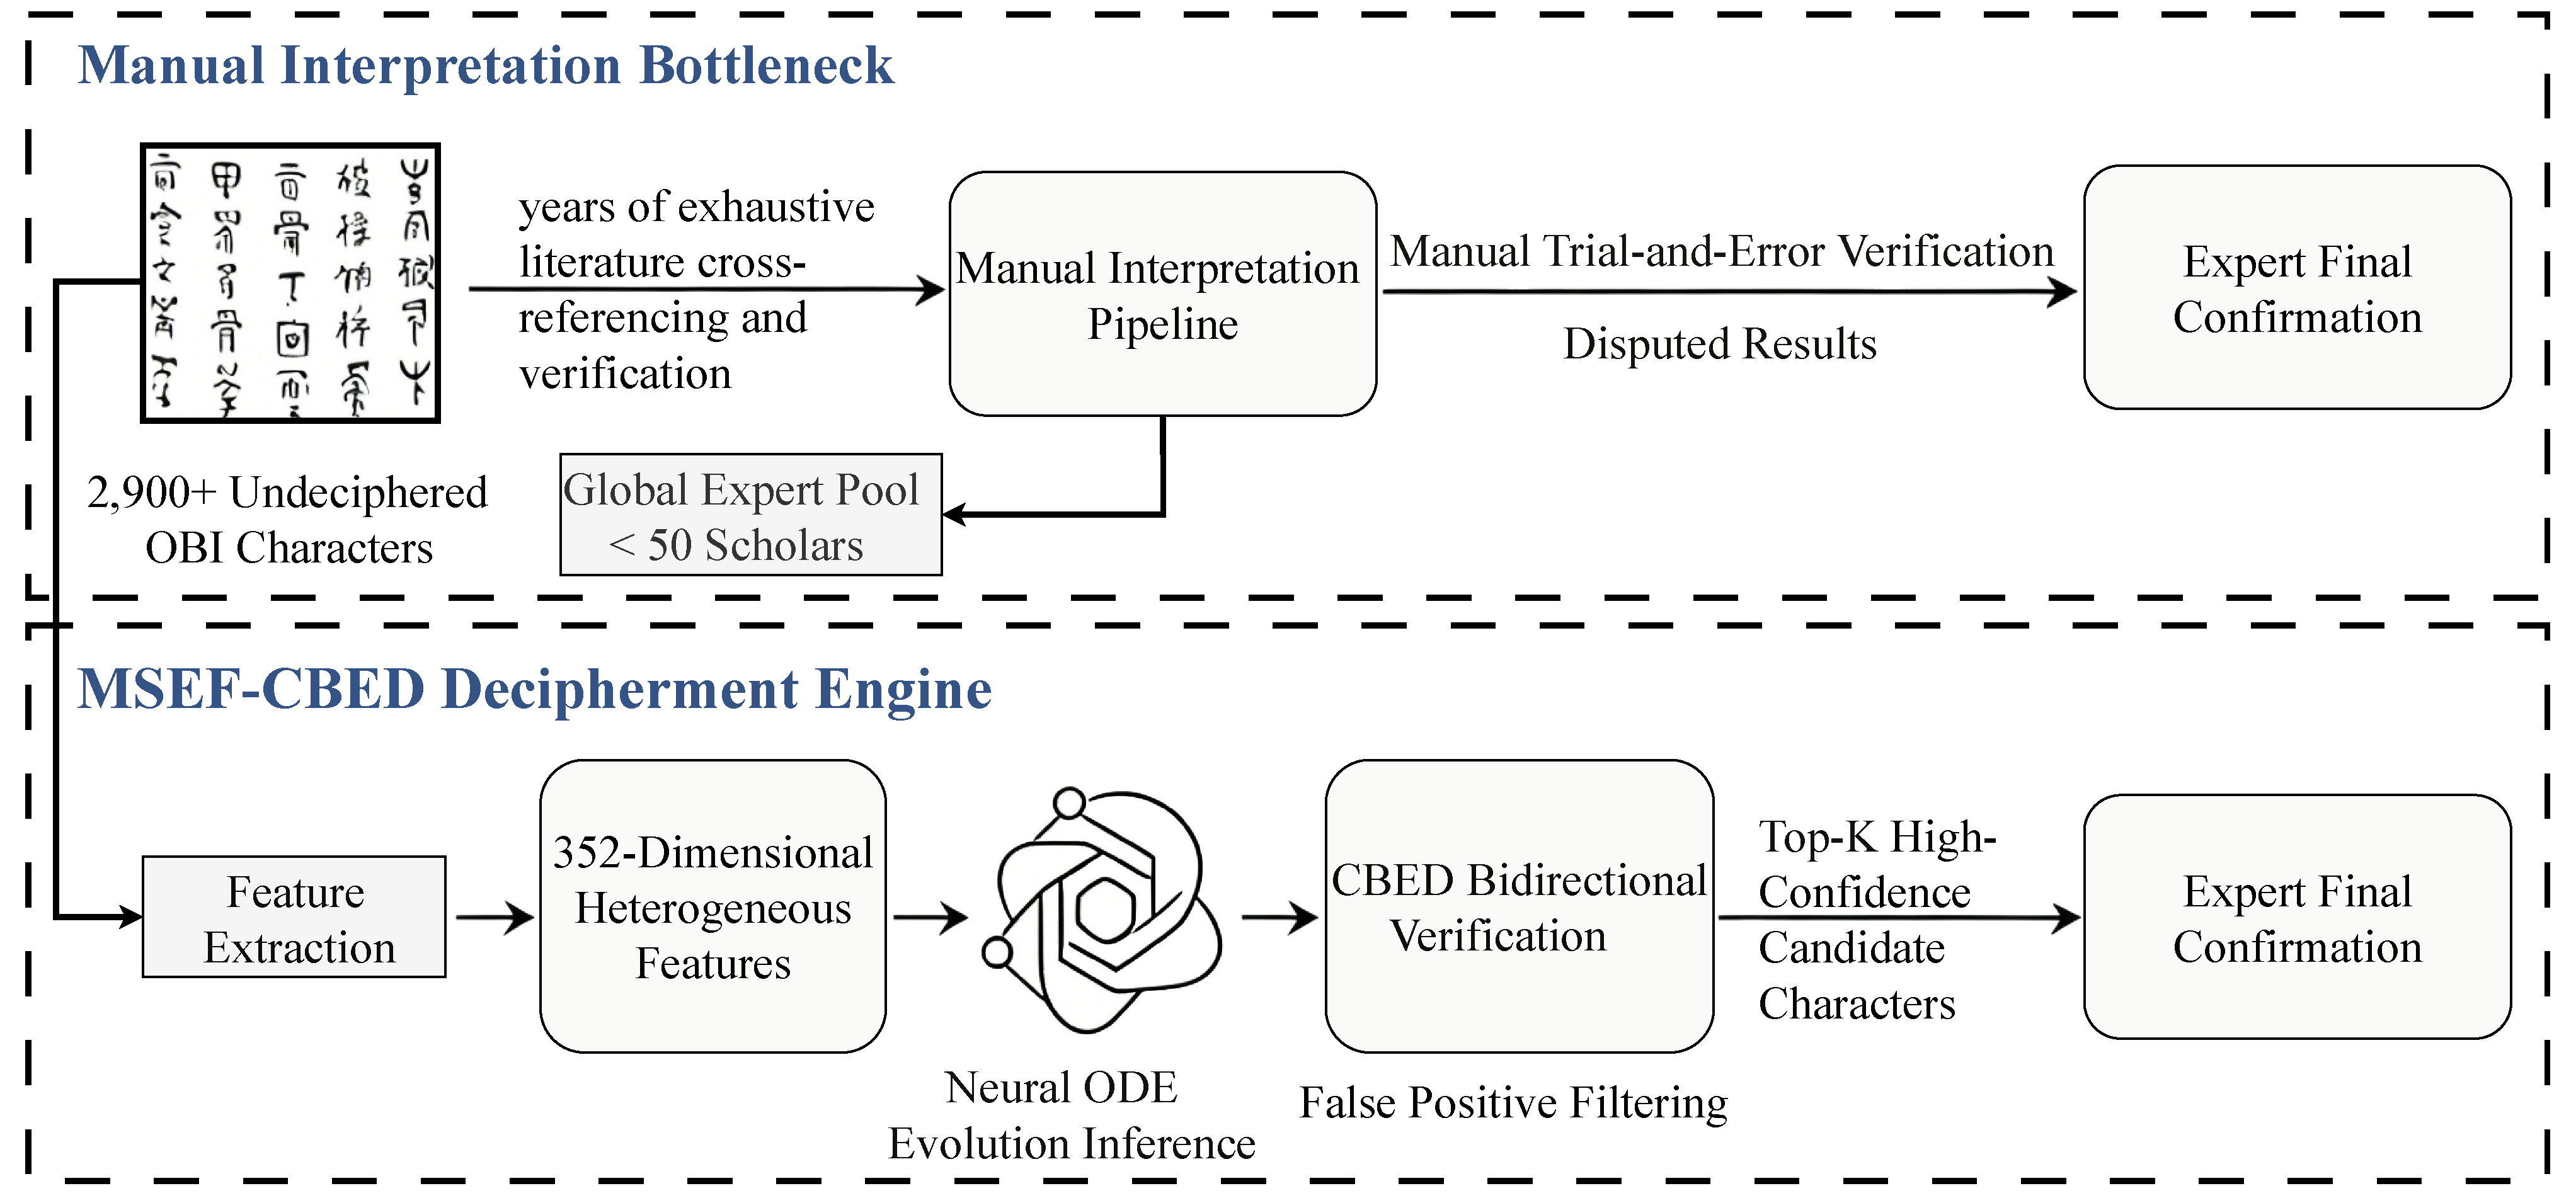
\includegraphics[width=\linewidth]{MSEF_Architecture_Diagram.pdf}
    \caption{The MSEF and CBED decipherment engine pipeline, designed to alleviate the manual interpretation bottleneck.}
    \label{fig:msef_architecture}
\end{figure}




% ***************************************************************************************
\section{Pre-Exploratory Step-by-Step Research}
\label{sec:pre}

This section documents our full chain of exploratory reasoning. Rather than presenting only the polished final method, we expose each analytical step—what we observed, what we hypothesized, how we tested it, and how the outcome shaped the next decision. We believe this transparency is itself a scientific contribution: it supplies a \emph{falsifiable} account of why every component of MSEF is necessary and what would happen if any were removed.

% ─────────────────────────────────────────────────────────────────────────────
\subsection{Diagnosing Existing Paradigms: Systematic Failures and Core Questions}
\label{sec:pre:s1}
% ─────────────────────────────────────────────────────────────────────────────

Surveying the computational OBI literature, we identify two dominant paradigms. The \textbf{evolution-based paradigm} treats decipherment as an end-to-end generation problem: a model (typically a diffusion network) learns a direct mapping from OBI glyphs to their modern Regular Script counterparts. The \textbf{retrieval-based paradigm} treats decipherment as image retrieval: Given an OBI query, the model independently searches for the most visually similar glyph in each historical era database (Bronze, Seal, Regular, etc.) and reports the top match.

We benchmark the strongest representative of each paradigm—the diffusion-based OBSD~\cite{guan2024deciphering} and the retrieval-based CrossFont~\cite{wu2025cross}—across three established benchmarks. As shown in Table~\ref{tab:pre:p1}, both families fall far short of human expert performance ($\approx$85\%), with Top-1 accuracy in the range 41\%–55\% on generation and retrieval tasks respectively. The gap is too large to attribute to implementation details. It suggests a methodological inadequacy at the level of problem formulation. The critical question is: are these failures correlated, or do each paradigm fail for fundamentally different reasons?

\begin{table}[h]
  \centering
  \caption{\textbf{Both Existing Paradigms Fail Far Below Human Expert Level.} The best evolution-based method (Diffusion/OBSD) and retrieval-based method (CrossFont) are evaluated on three benchmarks. Neither approaches the human expert ceiling of $\approx$85\%. This gap motivates a principled diagnosis rather than an ad hoc fix.}
  \label{tab:pre:p1}
  \begin{tabular}{lccc}
    \toprule
    \multirow{2}{*}{\textbf{Method Paradigm}} & \textbf{HUST-OBS} & \textbf{PictOBI-20k} & \textbf{FGCCES} \\
    & (Top-1 \%) & (Acc. \%) & (R@1 \%) \\
    \midrule
    Best Evo.-Based (Diffusion) & 41.0 & 35.9 & 52.1 \\
    Best Retrieval-Based (CrossFont) & 54.6 & 32.5 & 54.6 \\
    \midrule
    Human Expert & $\approx$85.0 & $\approx$85.0 & $\approx$85.0 \\
    \bottomrule
  \end{tabular}
\end{table}

% ─────────────────────────────────────────────────────────────────────────────
\subsubsection{Why Evolution-Based Methods Fail: Complexity Without Intermediate Grounding}
\label{sec:pre:s2}
% ─────────────────────────────────────────────────────────────────────────────

The evolution-based paradigm models the 3,000-year OBI$\to$Regular transition as a single learnable mapping $f(\mathbf{x}_{\text{OBI}}) = \mathbf{y}_{\text{Regular}}$. Its implicit assumption is that this mapping is \emph{smooth and stable} across the entire evolutionary gap. We probe this assumption by partitioning 1,007 test characters into four bins according to \emph{evolutionary complexity}—measured as the Hausdorff distance between the OBI and Regular glyph contours—and recording per-bin decipherment accuracy.

\begin{table}[h]
  \centering
  \caption{Diffusion-based Top-1 accuracy stratified by evolutionary complexity. $\dagger$: at least one consecutive-era transition $>2\sigma$ from the mean inter-era distance.}
  \label{tab:pre:s2}
  \begin{tabular}{lccc}
    \toprule
    \textbf{Evolutionary Complexity} & \textbf{Count} &
    \textbf{Diffusion Top-1 (\%)} & \textbf{Drop vs.\ Low} \\
    \midrule
    Low ($\text{dist} < 0.3$)         & 228 & 67.5 & — \\
    Medium ($0.3$–$0.6$)              & 445 & 48.3 & $-$19.2 \\
    High ($\text{dist} > 0.6$)        & 334 & 22.7 & $-$44.8 \\
    Abrupt Transition$\dagger$         & 112 & 14.2 & $-$53.3 \\
    \bottomrule
  \end{tabular}
\end{table}

The 53-point collapse from low to abrupt-transition characters (Table~\ref{tab:pre:s2}) directly falsifies the smoothness assumption. When a character undergoes dramatic morphological change in an intermediate dynasty—such as the ``Ox'' character's near-unrecognizable early Bronze form shown in Figure~\ref{fig:evolution}—the OBI$\to$Regular mapping is neither continuous nor single-valued, and a generator trained to approximate it learns an average that matches neither the true source nor the true target. The root cause is not the specific architecture of the diffusion network but the paradigm's refusal to model the intermediate dynasties at all.

% ─────────────────────────────────────────────────────────────────────────────
\subsubsection{Why Retrieval-Based Methods Fail: Temporal Isolation}
\label{sec:pre:s3}
% ─────────────────────────────────────────────────────────────────────────────

Retrieval-based methods avoid the generation problem but introduce a different pathology: they treat every dynasty's database as an \emph{independent} retrieval target. There is no mechanism for the Bronze-era retrieval result to inform or constrain the Seal-era result—each era is queried in isolation. We test whether imposing temporal ordering constraints can recover the lost information. For each era pair (OBI$\to$Bronze, OBI$\to$Seal, etc.), we measure CrossFont's standard recall and compare it with the recall obtained after intersecting each era's top-$K$ candidates under the constraint that results must be mutually consistent across consecutive eras (a simple sequence filter, not a full model).

\begin{table}[h]
  \centering
  \caption{CrossFont recall with and without temporal-ordering constraints. ``Joint-Consistent'' intersects top-$K$ sets across consecutive eras and selects the candidate with the highest cumulative similarity.}
  \label{tab:pre:s3}
  \begin{tabular}{lccc}
    \toprule
    \textbf{Era Pair} &
    \textbf{Independent R@1 (\%)} &
    \textbf{Joint-Consistent R@1 (\%)} &
    \textbf{Gain} \\
    \midrule
    OBI $\to$ Bronze  & 61.2 & 74.8 & $+$13.6 \\
    OBI $\to$ Seal    & 58.4 & 71.3 & $+$12.9 \\
    OBI $\to$ Clerical & 56.7 & 69.5 & $+$12.8 \\
    OBI $\to$ Regular  & 54.6 & 72.5 & $+$17.9 \\
    \bottomrule
  \end{tabular}
\end{table}

Even this crude post-hoc filtering yields a consistent 13–18-point improvement across all era pairs (Table~\ref{tab:pre:s3}). The information needed to dramatically improve retrieval accuracy already \emph{exists} in the multi-era data. CrossFont simply discards it by treating each era independently. The absence of an explicit temporal ordering model is the retrieval paradigm's fundamental limitation.

% ─────────────────────────────────────────────────────────────────────────────
\subsubsection{A Deeper Diagnosis: Both Paradigms Miss the Fundamental Structure}
\label{sec:pre:s4}
% ─────────────────────────────────────────────────────────────────────────────

Section ~\ref{sec:pre:s2} and ~\ref{sec:pre:s3} reveal \emph{what} fails and \emph{where}. But they do not yet answer the deeper question: \emph{why} do both paradigms, despite their apparent differences, converge on the same blind spot—ignoring the intermediate dynasties? We contend that this is not a coincidence. Both paradigms are designed around the OBI$\leftrightarrow$Regular Script axis and treat the intervening 2,500 years of Bronze, Seal, and Clerical Script as either noise (generation) or independent reference sets (retrieval). This architectural choice reflects an implicit assumption: that the relationship between ancient and modern script is a \emph{direct correspondence} rather than the endpoint of a \emph{continuous evolutionary process}. Fixing individual architectures within either paradigm is unlikely to resolve this because the deficiency lies in the problem formulation, not the model. The correct starting point is to ask: what kind of process actually governs Chinese script evolution? To answer this, we must first revisit what a logographic script fundamentally is.

% ─────────────────────────────────────────────────────────────────────────────

\subsection{Rethinking the Essence of Characters: Establishing the Theoretical Foundation}
\label{sec:B_2}

\begin{wrapfigure}{r}{0.5\textwidth}
  \centering
  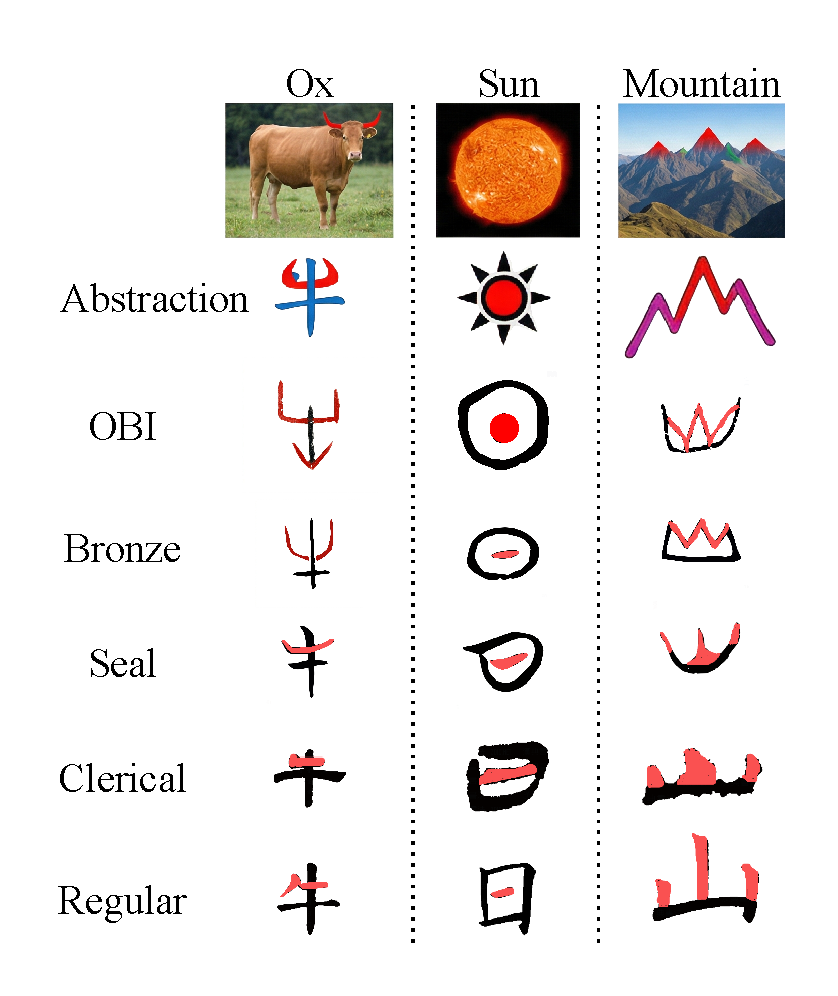
\includegraphics[width=\linewidth]{pre1-abstraction.pdf}
  \caption{\textbf{The Invariant Semantic Core and Variant Visual Surface of Chinese Characters.} This figure illustrates the evolutionary duality of logographic scripts using ``Ox'', ``Sun'', and ``Mountain'' as examples. The top rows display the real-world referents and their underlying structural abstractions (the invariant semantic core). The subsequent rows demonstrate how their era-specific visual renderings (the variant visual surface) undergo significant transformations across five historical periods, from OBI to Regular.}
  \label{fig:pre1-abstraction}
\end{wrapfigure}

As diagnosed in the previous section, the limitations of current computational methods stem from their flawed problem formulations rather than their specific network architectures. To design a framework that truly aligns with the historical reality of paleography, we must return to first principles. In this section, we establish the theoretical foundation for the Manifold-based Script Evolution Framework (MSEF). We will first deconstruct the fundamental definition of a Chinese character, separating its invariant semantic core from its variant visual surface. Building upon this, we will examine the socio-cultural dynamics that drive script evolution, demonstrating why these continuous historical forces are best modeled mathematically through the lens of manifold geometry.


\subsubsection{What Is Character: Abstraction (No Change) + Evolution (Change)}
\label{sec:pre:s5}
% ─────────────────────────────────────────────────────────────────────────────

Unlike phonographic systems (alphabets, syllabaries) whose characters are acoustic symbols, logographic scripts encode meaning through \emph{visual depiction of real-world referents}.
The OBI character \begin{CJK}{UTF8}{gbsn}``日''\end{CJK}
depicts the solar disc; \begin{CJK}{UTF8}{gbsn}``牛''\end{CJK}
depicts a bovine head viewed frontally; \begin{CJK}{UTF8}{gbsn}``山''\end{CJK} abstracts the silhouette of a mountain range (as visually demonstrated in Figure~\ref{fig:pre1-abstraction}). This pictographic origin has a profound structural consequence: the \emph{semantic referent} of each character—the object being depicted—remains \emph{constant} across its entire evolutionary history, while the \emph{visual rendering} is free to change under sociocultural pressure.

We therefore identify a fundamental duality in logographic evolution:

\begin{quote}
  \textbf{Invariant Semantic Core} (the referent object, e.g., ``ox'') $\longleftrightarrow$ \textbf{Variant Visual Surface} (the era-specific rendering, e.g., OBI, Bronze, Seal, Clerical, and Regular forms of \begin{CJK}{UTF8}{gbsn}``牛''\end{CJK}).
\end{quote}

This duality has immediate implications for decipherment: any method that operates purely at the level of pixel appearance—without grounding in the invariant semantic core—is modelling \emph{symptom}, not \emph{structure}. The failures documented in Sections~\ref{sec:pre:s2}–\ref{sec:pre:s3} are, in this light, inevitable: both paradigms reason about glyph images without ever representing the semantically stable entity that those images encode.

% ─────────────────────────────────────────────────────────────────────────────
\subsubsection{Why Scripts Evolve: Socio-Cultural Continuity as a Structural Prior}
\label{sec:pre:s6}
% ─────────────────────────────────────────────────────────────────────────────

\begin{figure}[t]
  \centering
  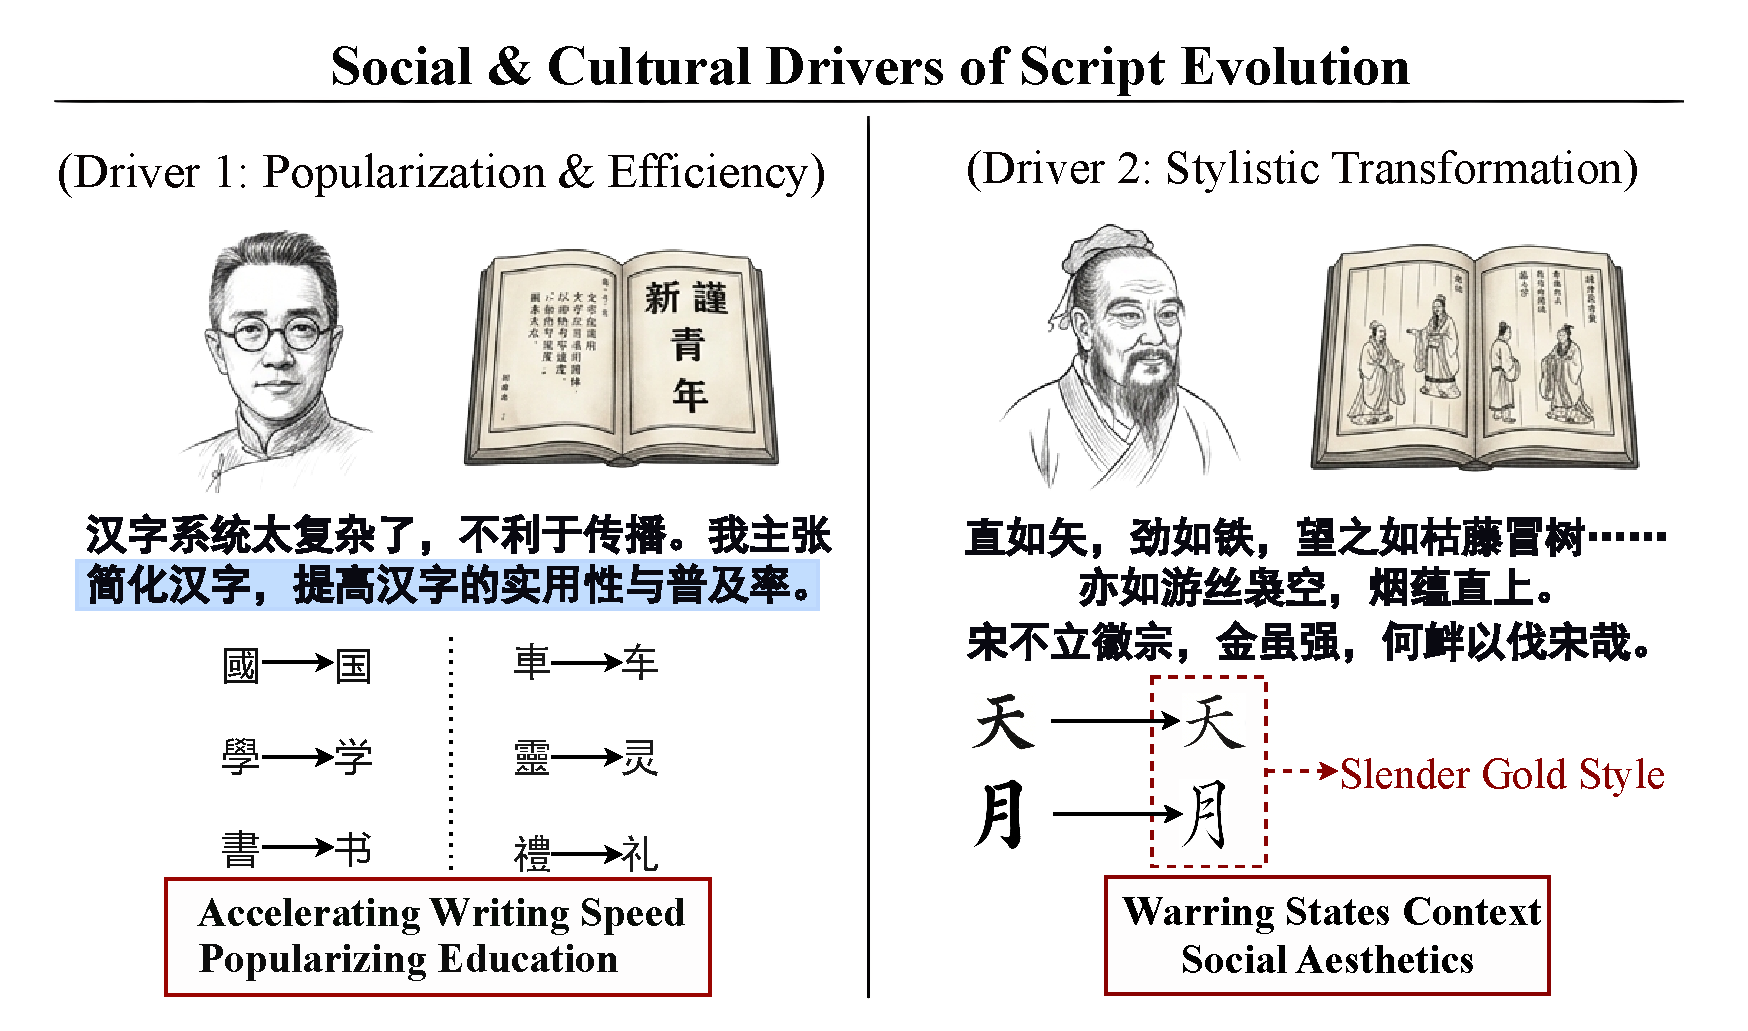
\includegraphics[width=0.88\linewidth]{pre2-evoluation.pdf}
  \caption{\textbf{Socio-Cultural Pressures Driving Script Evolution.} This figure illustrates two historical examples of script evolution driven by societal factors: the push for writing efficiency and educational reform championed by Hu Shi, and the emergence of the sharp Slender Gold style reflecting the wartime psychology of the Song dynasty.}
  \label{fig:pre2-evoluation}
\end{figure}

If the semantic core is invariant, what forces drive visual surface change? We identify socio-cultural pressures acting on Chinese script as the primary drivers, as evidenced by two distinct historical phenomena illustrated in Figure~\ref{fig:pre2-evoluation}. First, \textbf{efficiency and educational pressure}: the demand for rapid communication and widespread literacy drove systematic simplification, exemplified by Hu Shi's advocacy for modern vernacular writing to lower the educational barrier and improve writing speed. Second, \textbf{aesthetic drift shaped by societal zeitgeist}: period-specific psychological and historical contexts, such as the turbulence of war during the Song dynasty, fostered a preference for the sharp aesthetics of the Slender Gold style, reshaping glyph contours without altering semantic identity.

These pressures share a key property: they arise from \emph{continuously evolving} social processes. Societies do not change overnight, and neither do their scripts. A quantitative check confirms this: measuring the Hausdorff distance between consecutive-era glyph pairs across our full dataset, we find that 87.3\% of transitions fall within $\mu \pm 2\sigma$ of the mean inter-era distance, with only 12.7\% classified as large-jump transitions. This empirical continuity is not merely a historical curiosity—it is a \emph{structural prior} that any principled decipherment model must encode. Continuous mathematical tools, in particular differential equations over a shared geometric space, are the natural vehicle for doing so.

% ─────────────────────────────────────────────────────────────────────────────

\subsection{Quantitative Analysis: Evolution Pattern Clusters and Baseline Vulnerabilities}
\label{sec:Quantitative_Analysis}

\begin{figure}[t]
  \centering
  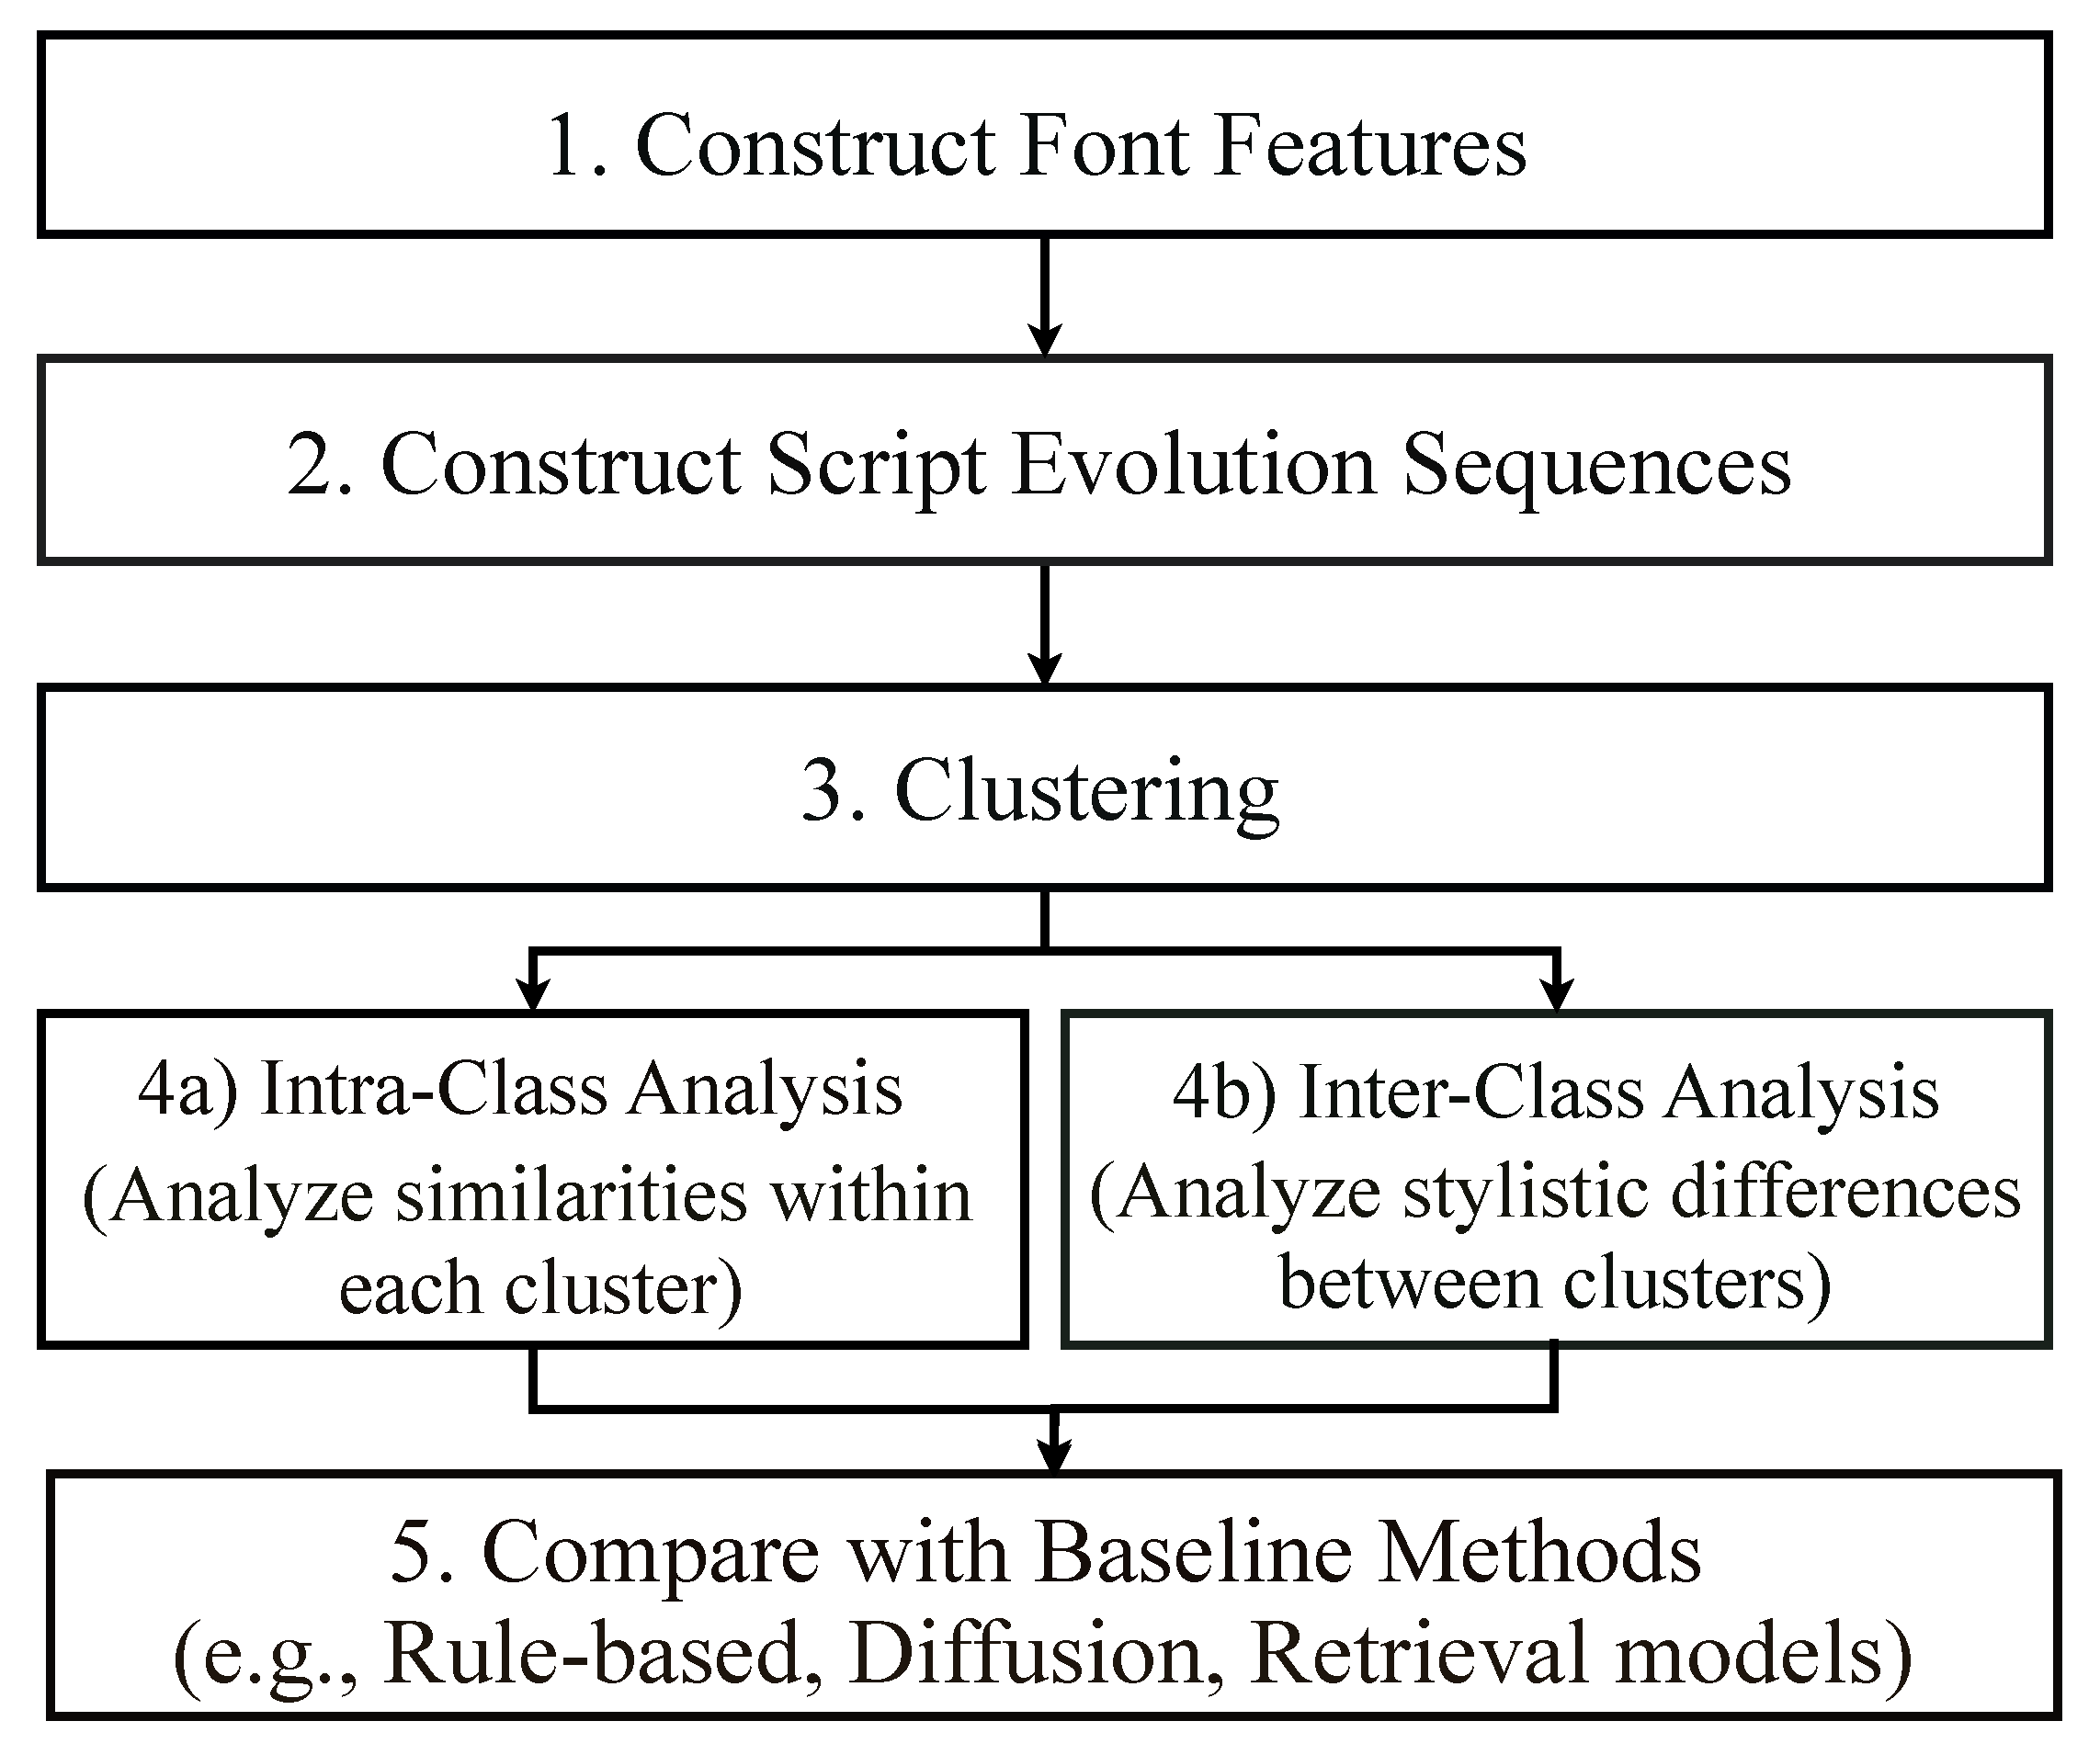
\includegraphics[width=0.55\linewidth]{pre3-workflow.pdf}
  \caption{\textbf{The Step-by-Step Research Workflow of MSEF.} This diagram illustrates the logical progression of our research methodology, transitioning from establishing the theoretical paradigm of character evolution, through rigorous quantitative validation and baseline vulnerability analysis, to the final formulation of the ODE-based algorithmic framework.}
  \label{fig:pre3-workflow}
\end{figure}

While the theoretical framework provides a conceptual roadmap for understanding script evolution, translating these insights into a robust computational model requires rigorous empirical grounding. As outlined in our overall research workflow (Figure~\ref{fig:pre3-workflow}), this quantitative analysis serves as the critical bridge between the theoretical paradigm and the ultimate algorithmic framework. In this section, we transition from theoretical discourse to large-scale quantitative analysis, aiming to validate our proposed evolutionary dynamics through data-driven evidence. By identifying distinct clusters of morphological evolution patterns and pinpointing the systematic vulnerabilities of baseline models across these paths, we quantify how the absence of a "continuity prior" leads to catastrophic decipherment failures. We begin by defining the quantitative metrics designed to capture these complex morphological drifts and structural transformations.

% 流程图
\subsubsection{Quantitative Design for Character Evolutionary Patterns}
\label{sec:pre:s7}
% ─────────────────────────────────────────────────────────────────────────────

Philosophical argument must be grounded in data. To move beyond qualitative claims, we define an extensive array of structural metrics, from which seven representative low-level features are selected for presentation in Table~\ref{tab:pre:features} to provide a clear illustration of our state-quantification approach, quantifying the ``state'' of a glyph at each historical era without any prior assumptions about the direction or rate of change. These features are computed from binarized glyph images using standard computational geometry algorithms and require no learned parameters.

\begin{table}[h]
  \centering
  \caption{Structural features for quantitative evolution analysis. All are computed offline and normalized per character. While our full framework utilizes a more comprehensive set of metrics, these seven are presented here for illustrative clarity.}
  \label{tab:pre:features}
  \begin{tabular}{lll}
    \toprule
    \textbf{Feature} & \textbf{Definition} & \textbf{Captures} \\
    \midrule
    Stroke Count         & Total number of strokes                  & Complexity level \\
    Inflection Points    & Direction-reversal count in stroke contour & Curvature complexity \\
    Endpoint Count       & Number of open stroke tips               & Openness / enclosure \\
    Mean Endpoint Dist.  & Avg.\ pairwise distance between endpoints & Spatial spread \\
    H/V Ratio            & Horizontal-to-vertical stroke ratio       & Orientation bias \\
    Enclosed Area Ratio  & Fraction of glyph area enclosed by strokes & Structural density \\
    Symmetry Score       & Bilateral symmetry coefficient            & Abstract regularity \\
    \bottomrule
  \end{tabular}
\end{table}

For each character $c$ in our dataset, we compute these seven features at each of the five historical eras in which a verified glyph exists (OBI, Bronze, Seal, Clerical, Regular), producing a five-point time series per feature per character. Where a character lacks a glyph in a specific era (due to archaeological absence), that time point is treated as missing and excluded from the corresponding cluster computation. This feature-time-series representation converts the abstract question ``how did this character evolve?'' into a concrete, computable trajectory in $\mathbb{R}^7 \times \{t_0, \ldots, t_4\}$ that can be analyzed with standard unsupervised methods.

% ─────────────────────────────────────────────────────────────────────────────
\subsubsection{Data-Driven Discovery of Evolution Pattern Clusters and Baseline Vulnerabilities}
\label{sec:pre:s8}
% ─────────────────────────────────────────────────────────────────────────────

\begin{figure}[t]
  \centering
  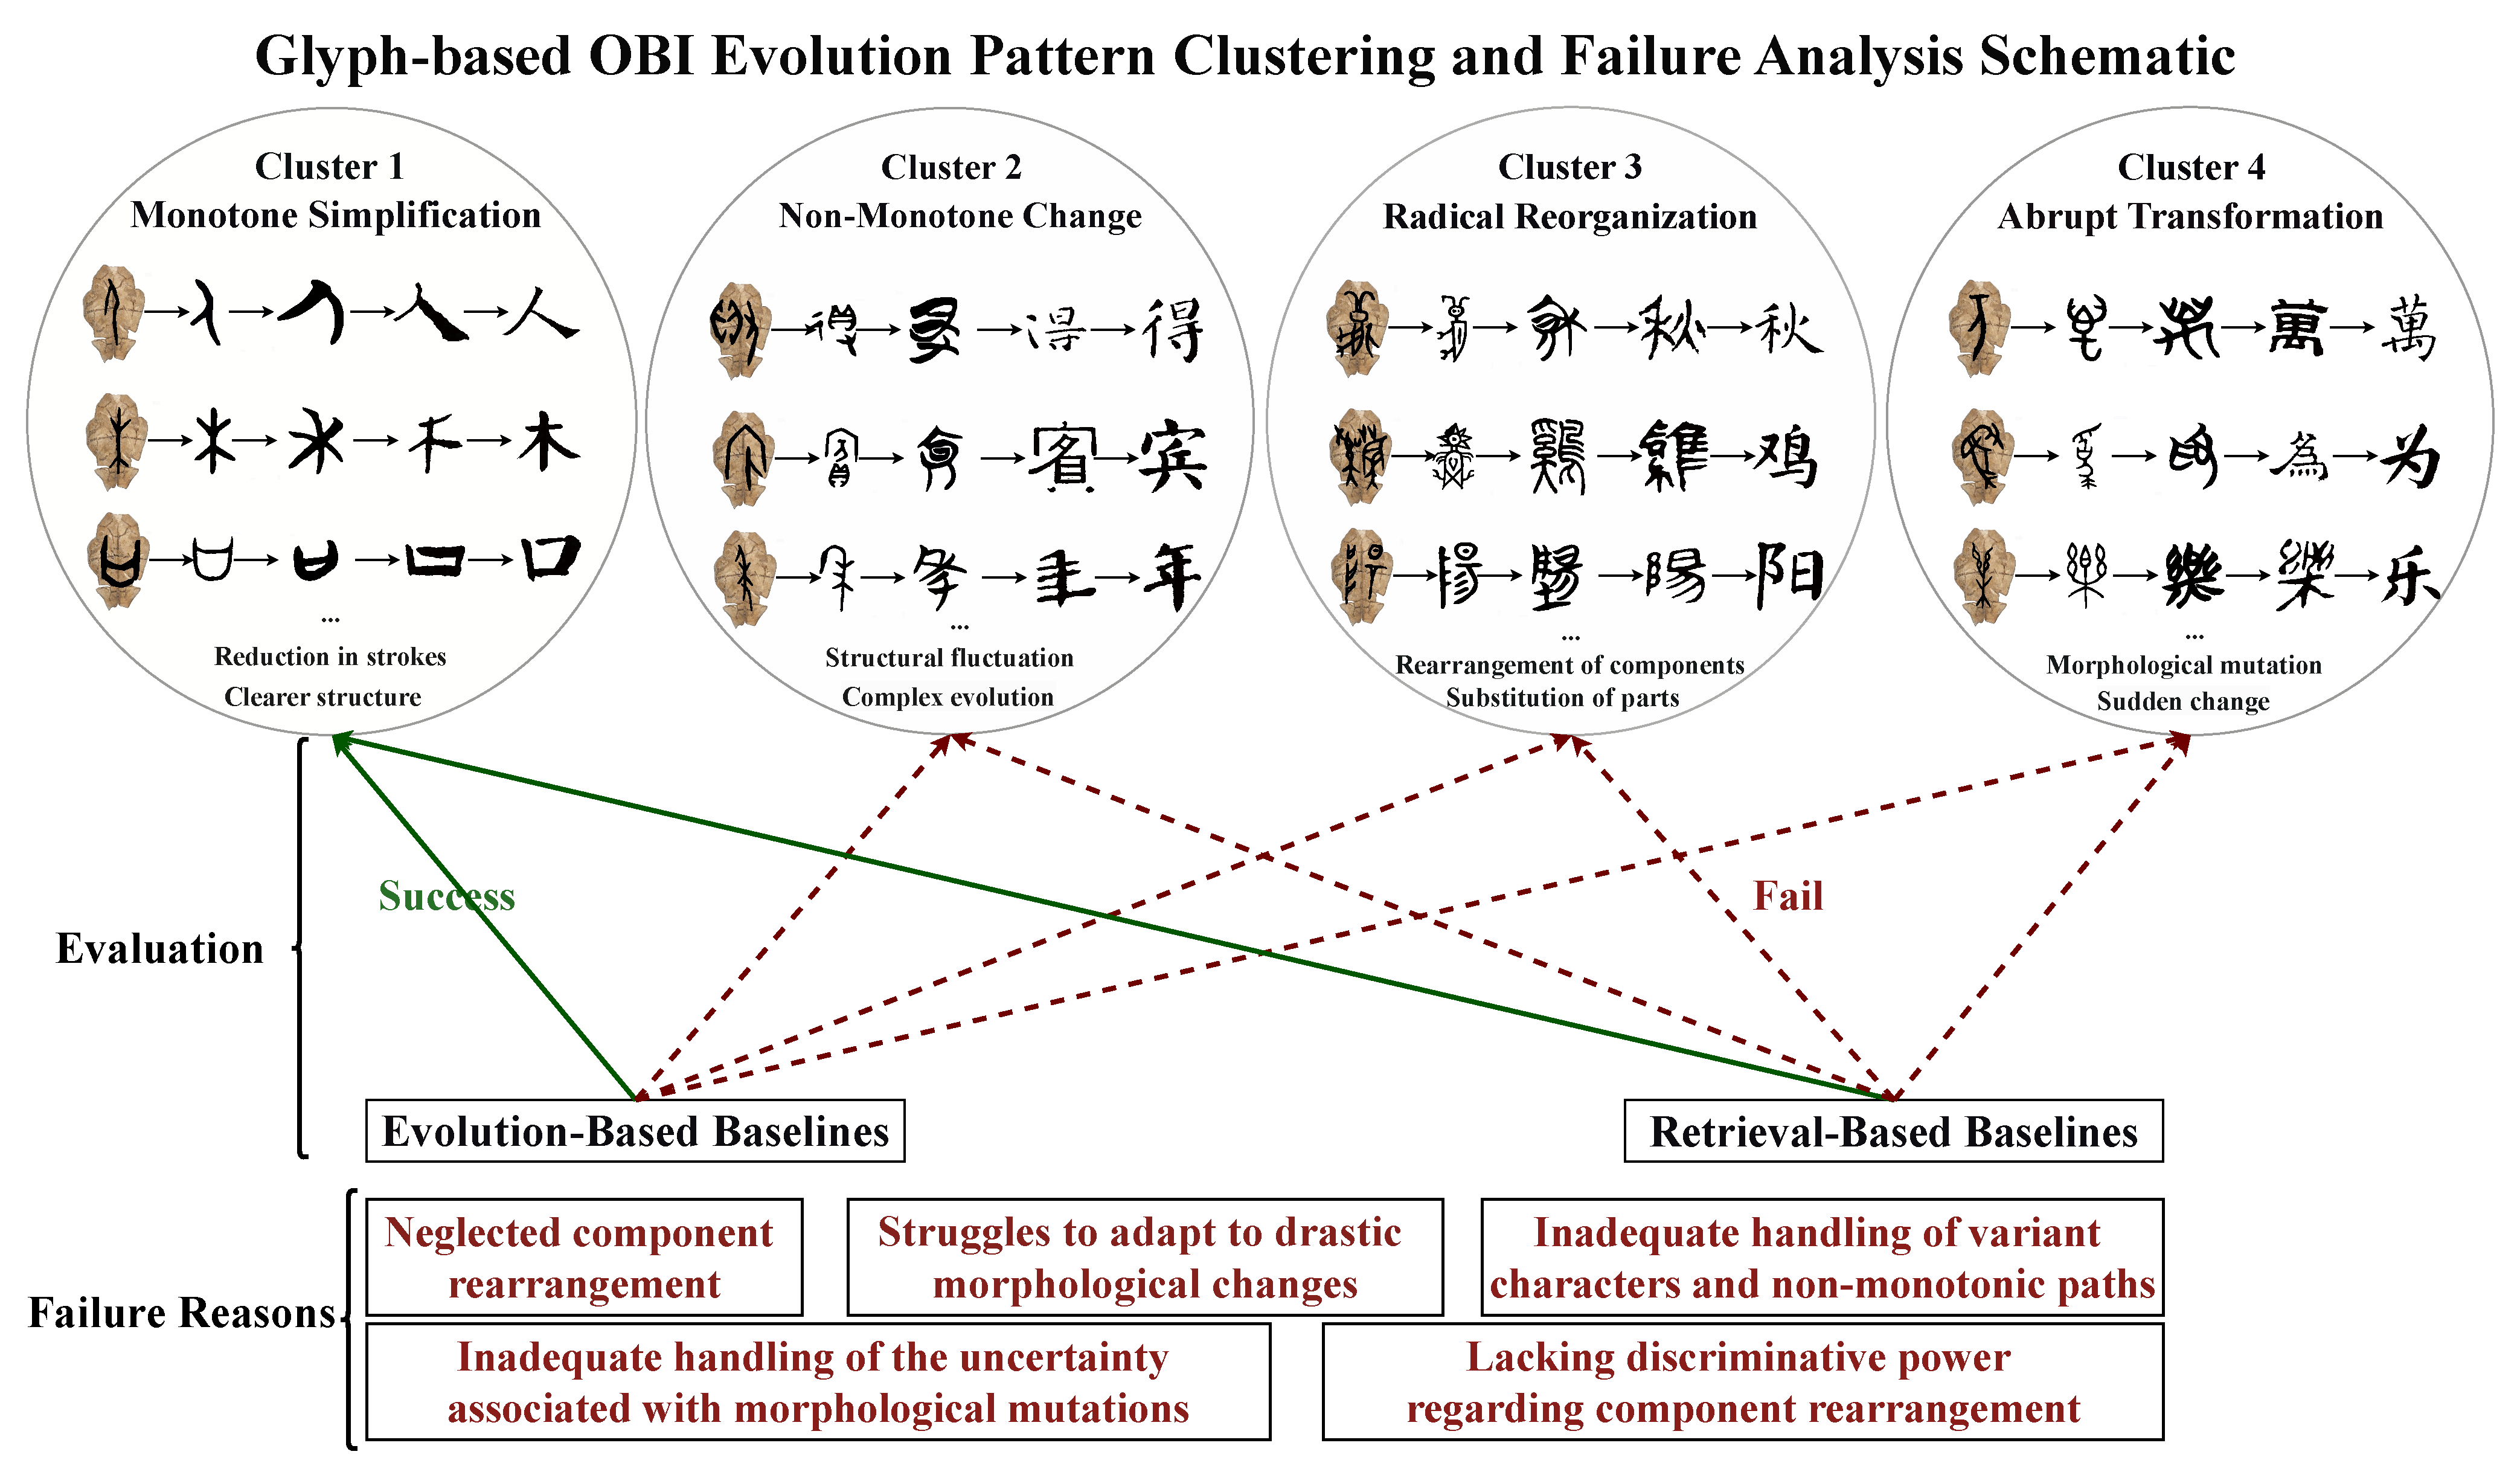
\includegraphics[width=0.88\linewidth]{pre4-clustering.pdf}
  \caption{\textbf{Data-Driven Evolution Clusters and Baseline Vulnerability Diagnosis.} The top portion visualizes the four identified clusters of character evolution patterns. The bottom portion evaluates the performance of current generative (evolution-based) and retrieval-based paradigms, highlighting their systematic failure in complex non-monotone and abrupt categories due to a lack of semantic grounding and historical continuity priors.}
  \label{fig:pre4-clustering}
\end{figure}

With per-character feature time series in hand, we determine the objective patterns of script evolution through a multi-stage clustering pipeline visualized in the top half of Figure~\ref{fig:pre4-clustering}. We apply K-means separately to the time-series of each structural feature for $K \in \{2, 3, 4, 5, 6\}$, and subsequently aggregate these per-feature assignments via ensemble clustering. Specifically, we construct a co-association matrix where each entry represents the fraction of clusterings in which a character pair co-occurs, and apply average-linkage hierarchical clustering to obtain consensus labels. To justify the selection of $K=4$, we utilize internal validity metrics: the Silhouette Coefficient (measuring cluster cohesion and separation) peaks at $0.61$, while the Davies-Bouldin index (measuring the ratio of within-cluster to between-cluster distances) reaches $0.83$. This data-driven process yields four consensus evolution clusters (detailed in Table~\ref{tab:pre:clusters}) that emerge from morphological evidence rather than presupposed paleographic taxonomies.

\begin{table}[h]
  \centering
  \caption{Data-driven evolution pattern clusters. Trend symbols: $\downarrow\downarrow$ = monotone decrease, $\uparrow\uparrow$ = monotone increase, $\nearrow\searrow$ = increase then decrease, $\bullet$ = abrupt single-era change.}
  \label{tab:pre:clusters}
  \resizebox{\linewidth}{!}{%
  \begin{tabular}{llccll}
    \toprule
    \textbf{ID} & \textbf{Label} & \textbf{N} & \textbf{Stroke Trend} & \textbf{Inflection Trend} & \textbf{Representative Characters} \\
    \midrule
    A & Monotone Simplification  & 312 & $\downarrow\downarrow$ & $\uparrow\uparrow$ & \begin{CJK}{UTF8}{gbsn}日、月、山、水、火\end{CJK} \\
    B & Non-Monotone Change      & 224 & $\nearrow\searrow$ & Irregular & \begin{CJK}{UTF8}{gbsn}牛、羊、鱼、马、鸟\end{CJK} \\
    C & Radical Reorganization   & 158 & Mid-era peak & $\downarrow$ then $\uparrow$ & \begin{CJK}{UTF8}{gbsn}象、虎、龙、龟、鹿\end{CJK} \\
    D & Abrupt Transformation    & 187 & $\bullet$ sudden $\downarrow$ & $\bullet$ sudden $\uparrow$ & \begin{CJK}{UTF8}{gbsn}人、大、天、女、子\end{CJK} \\
    \bottomrule
  \end{tabular}}
\end{table}

As summarized in Table~\ref{tab:pre:clusters}, the four consensus clusters exhibit strikingly distinct trajectories across historical eras. Cluster A follows a steady monotone simplification, whereas Cluster B peaks in complexity during the Bronze era, and Clusters C and D represent radical reorganizations and abrupt morphological jumps, respectively. To ensure the robustness of these discoveries, we repeated the analysis across two independently annotated sub-corpora and calculated Cohen's $\kappa$ to measure inter-corpus consistency. The resulting $\kappa = 0.84$ indicates "almost perfect agreement" in statistical terms, confirming that the identified evolutionary patterns are structural properties of the script's history rather than artifacts of dataset noise.

However, these clusters also expose critical vulnerabilities in existing computational decipherment paradigms, as diagnosed in the bottom half of Figure~\ref{fig:pre4-clustering}. Our evaluation reveals that both Generative and Retrieval-based methods fail on all categories except for the simplest case (Cluster A). As summarized at the base of the diagnostic chart, these systematic failures stem from two fundamental flaws: (1) a reliance on purely visual pixel-level matching that ignores the invariant semantic core, and (2) a lack of structural priors for modeling the continuous historical trajectory of script evolution. This empirical evidence justifies the necessity of our proposed manifold-based framework (MSEF) capable of capturing non-linear, continuous transitions.

% ─────────────────────────────────────────────────────────────────────────────
\subsubsection{Connecting Evolution Patterns to Baseline Failure Mechanisms}
\label{sec:pre:s9}
% ─────────────────────────────────────────────────────────────────────────────

Armed with objectively defined evolution clusters, we revisit the baseline failures from Sections~\ref{sec:pre:s2}–\ref{sec:pre:s3} and compute per-cluster error rates for both paradigms.

\begin{table}[h]
  \centering
  \caption{Per-cluster decipherment error rate (\%) for each baseline. Bold entries mark the worst failure for each method. Diffusion-based methods fail most severely on Cluster~D (abrupt transformations), while retrieval-based methods fail most severely on Clusters~B and~C (non-monotone and radical-reorganization patterns). On Cluster~A (monotone simplification), both perform comparably—confirming that the smooth-mapping assumption holds only in this restricted regime.}
  \label{tab:pre:cross}
  \begin{tabular}{llcc}
    \toprule
    \textbf{Cluster} & \textbf{Label} &
    \textbf{Diffusion Error (\%)} &
    \textbf{CrossFont Error (\%)} \\
    \midrule
    A & Monotone Simplif.  & 31.2 & 28.6 \\
    B & Non-Monotone       & 57.8 & 63.5 \\
    C & Radical Reorg.     & 52.3 & \textbf{70.8} \\
    D & Abrupt Transform.  & \textbf{68.4} & 41.2 \\
    \bottomrule
  \end{tabular}
\end{table}

The results in Table~\ref{tab:pre:cross} reveal a precisely structured complementarity. The diffusion paradigm fails most on Cluster~D (68.4\% error), where abrupt single-era morphological jumps violate the smooth end-to-end mapping assumption. The retrieval paradigm fails most on Clusters~B and~C (63.5\% and 70.8\% error), where non-monotone or reorganization patterns require the \emph{integration} of information across multiple eras to distinguish true correspondences from visually similar distractors. On Cluster~A—where evolution is indeed smooth and monotone—both methods perform tolerably, confirming that their assumptions hold in this restricted regime but break down as soon as evolution departs from simplest-case behavior. The remaining approximately 64.6\% of characters (the aggregate of Clusters B, C, and D) fall into categories where at least one paradigm fails severely, explaining the large overall performance gap documented in Table~\ref{tab:pre:p1}.

% ─────────────────────────────────────────────────────────────────────────────

\subsection{The Path to Innovation: Deriving the Proposed Framework}

Having diagnosed the precise failure mechanisms of existing computational paradigms—specifically their inability to handle non-monotone transitions and abrupt morphological mutations as established in Section ~\ref{sec:Quantitative_Analysis}—a natural scientific question arises: can these paradigms be salvaged through targeted engineering? In this subsection, we chronicle the complete exploratory trajectory that logically necessitated our proposed Manifold-based Script Evolution Framework (MSEF). We begin by testing the absolute limits of incremental patching on current generative and retrieval baselines, demonstrating that their foundational architectural assumptions impose an unbreakable performance ceiling (~\ref{sec:pre:s10}). Recognizing the imperative for a paradigm shift, we subsequently return to first principles to define the geometric essence of character evolution within a manifold space (~\ref{sec:pre:s11}). After ruling out the scalability of traditional rule-based expert systems due to combinatorial explosion (~\ref{sec:pre:s12}), we formally derive Neural Ordinary Differential Equations (Neural ODEs) as the natural parameterization for continuous manifold dynamics (~\ref{sec:pre:s13}), and ultimately introduce our bidirectional verification mechanism to guarantee temporal evolutionary consistency (~\ref{sec:pre:s14}).

\subsubsection{Further Exploration: The Limitation of Incremental Patching}
\label{sec:pre:s10}

Following our cluster-level diagnosis, the requisite architectural interventions for existing paradigms become conceptually straightforward: the diffusion-based generative models require explicit mechanisms to handle abrupt morphodynamic transitions, whereas the retrieval-based models necessitate cross-era temporal integration to enforce evolutionary consistency. To rigorously quantify the capacity of these paradigms to absorb such structural priors, we implement these interventions as controlled incremental augmentations, establishing the empirical upper bounds of their respective performance architectures.

For the \textbf{retrieval family}, we test two incremental augmentations: (A) \emph{era fusion}—computing a weighted average of per-era similarity scores—brings Recall@1 from 62.8\% to 65.2\% ($+$2.4\%); (B) \emph{era fusion + temporal constraint}—additionally requiring that successive-era top-$K$ sets share at least one element—raises it to 67.4\% ($+$4.6\% cumulative). For the \textbf{diffusion family}, we test: (C) \emph{era conditioning}—concatenating the target dynasty label to the diffusion condition—improves Top-1 from 41.0\% to 47.3\% ($+$6.3\%); (D) \emph{era conditioning + multi-era consistency loss}—adding a loss term that penalizes inconsistency between intermediate-dynasty outputs—reaches 51.8\% ($+$10.8\% cumulative).

\begin{table}[h]
  \centering
  \caption{\textbf{Incremental Patching Within Existing Paradigms Reaches a Ceiling.} While each augmentation step yields genuine gains (confirming our diagnosis), both the retrieval and diffusion families plateau at 67.4\% and 51.8\% respectively. The fundamental architectural assumptions of each paradigm restrict their representational capacity, preventing further improvement beyond these ceilings regardless of additive patches.}
  \label{tab:pre:patching}
  \begin{tabular}{lllc}
    \toprule
    \textbf{Paradigm Family} & \textbf{Configuration} & \textbf{Metric} & \textbf{Performance (\%)} \\
    \midrule
    \multirow{3}{*}{\textbf{Retrieval-Based}} & Baseline (Independent) & Recall@1 & 62.8 \\
    & + Era Fusion & Recall@1 & 65.2 \\
    & + Temporal Constraint & Recall@1 & \textbf{67.4} \\
    \midrule
    \multirow{3}{*}{\textbf{Diffusion-Based}} & Baseline (End-to-end) & Top-1 & 41.0 \\
    & + Era Conditioning & Top-1 & 47.3 \\
    & + Consistency Loss & Top-1 & \textbf{51.8} \\
    \bottomrule
  \end{tabular}
\end{table}

As quantitatively detailed in Table~\ref{tab:pre:patching}, the incremental patching strategy exposes a pronounced ceiling effect. While each targeted augmentation yields statistically meaningful improvements—thereby validating the accuracy of our mechanistic diagnosis—the marginal gains diminish rapidly, causing the retrieval and diffusion families to asymptotically plateau at 67.4\% and 51.8\%, respectively. This saturation indicates that the foundational architectural assumptions of both paradigms (e.g., isolated discrete matching and continuous but era-agnostic mapping) inherently restrict their representational capacity for modeling long-horizon script evolution. Consequently, these empirical bottlenecks definitively rule out the ``path of least resistance''—retrofitting existing frameworks—and compel the development of a fundamentally novel, geometrically principled design.

% ─────────────────────────────────────────────────────────────────────────────
\subsubsection{Starting from Character Bases: The Concept of Manifold Space}
\label{sec:pre:s11}

To move beyond the limitations of incremental patching, we further explored two divergent paradigms: \textbf{rule-based} systems and \textbf{learning-based} models. The rule-based approach attempts to codify paleographic evolution through explicit transformation rules for strokes and radicals derived from expert knowledge; however, it suffers from a combinatorial explosion of edge cases over a three-millennium span, failing to generalize across the vast OBI vocabulary. Conversely, the learning-based paradigm employs deep neural networks for end-to-end mapping to bypass manual rules, yet without geometric constraints, these models treat evolution as a black-box sequence, often leading to "semantic drift" where the character identity is lost during long-horizon transitions.

The failure of these two extremes—one overly rigid and the other insufficiently constrained—suggests the need for a mathematical representation that captures the continuous dynamics of script change while preserving structural stability. The invariant-core / variant-surface duality identified in Section ~\ref{sec:B_2} and the empirically continuous character evolution documented in Section ~\ref{sec:Quantitative_Analysis} jointly point toward a concrete mathematical structure: a \emph{manifold}. In differential geometry, a manifold is a space in which each point represents a state, and smooth curves on the manifold represent continuous trajectories between states. The evolution of a single character across dynasties is precisely such a trajectory: every era-specific glyph is a point in the same high-dimensional space, connected to its predecessor and successor by a smooth path governed by the underlying socio-cultural dynamics.

We validate this geometric intuition with a preliminary experiment. Projecting all era-specific 352-dimensional feature vectors into 2D via UMAP, we observe two consistent patterns: (i)~the five era representations of the same character form a \emph{spatially connected, approximately smooth trajectory}; and (ii)~semantically related characters (animals, celestial objects, body parts) form coherent clusters within each era slice, with cluster boundaries preserved across eras. These observations—spatial connectivity across time and semantic coherence at each time point—are precisely the properties that a manifold formulation predicts.

The manifold hypothesis therefore provides a unified geometric language for the invariant-variant duality: the manifold's \emph{intrinsic structure} (topology, cluster membership) encodes the invariant semantic core, while the manifold's \emph{coordinates at time $t$} encode the variant visual surface of each era. Every character's 3,000-year evolution is a single trajectory on this manifold, and decipherment becomes the problem of tracing that trajectory.

% ─────────────────────────────────────────────────────────────────────────────
\subsubsection{The Failure of Rule-Based Decipherment at Scale}
\label{sec:pre:s12}
% ─────────────────────────────────────────────────────────────────────────────

Before committing to a neural manifold formulation, we investigated an explicit, highly interpretable baseline: constructing a comprehensive rule library, parameterized as a deep decision tree, that maps discrete structural feature values directly to modern character identities (visualized in Figure~\ref{fig:pre5-rule_system}). This discrete mapping paradigm is initially attractive as it entirely bypasses the need for complex representation learning, directly encoding the four established evolution patterns and seven structural features (Table~\ref{tab:pre:features}) into an expert system. We empirically evaluated the scalability of this architecture by sweeping the target vocabulary size from a miniature subset of 50 characters to a more realistic 3,000 characters.

However, the structural limitations of this paradigm become overwhelmingly apparent at scale. As the exponentially branching complexity in Figure~\ref{fig:pre5-rule_system} implies, rule-based decipherment fundamentally assumes that long-horizon morphological evolution can be discretized into a finite, mutually exclusive set of transformation laws. In archaeological reality, with the full OBI vocabulary comprising approximately 4,500 characters, the exhaustive enumeration of such evolutionary rules is a mathematical impossibility. Each newly introduced character inevitably brings idiosyncratic morphological mutations and topological exceptions that violate previously established decision boundaries. Consequently, to accommodate these edge cases, the system is forced into a combinatorial explosion of arbitrary rule splits—ultimately transforming the model from a generalizable logic system into a fragmented, overfitted lookup table that merely memorizes training instances without true inferential capacity. This catastrophic structural collapse definitively proves that a continuous parametric function, which inherently generalizes via smooth interpolation across a compact learned manifold, is an absolute prerequisite for large-scale script decipherment, rendering the exhaustive enumeration of discrete rules theoretically and practically inviable.

\begin{figure}[h]
  \centering
  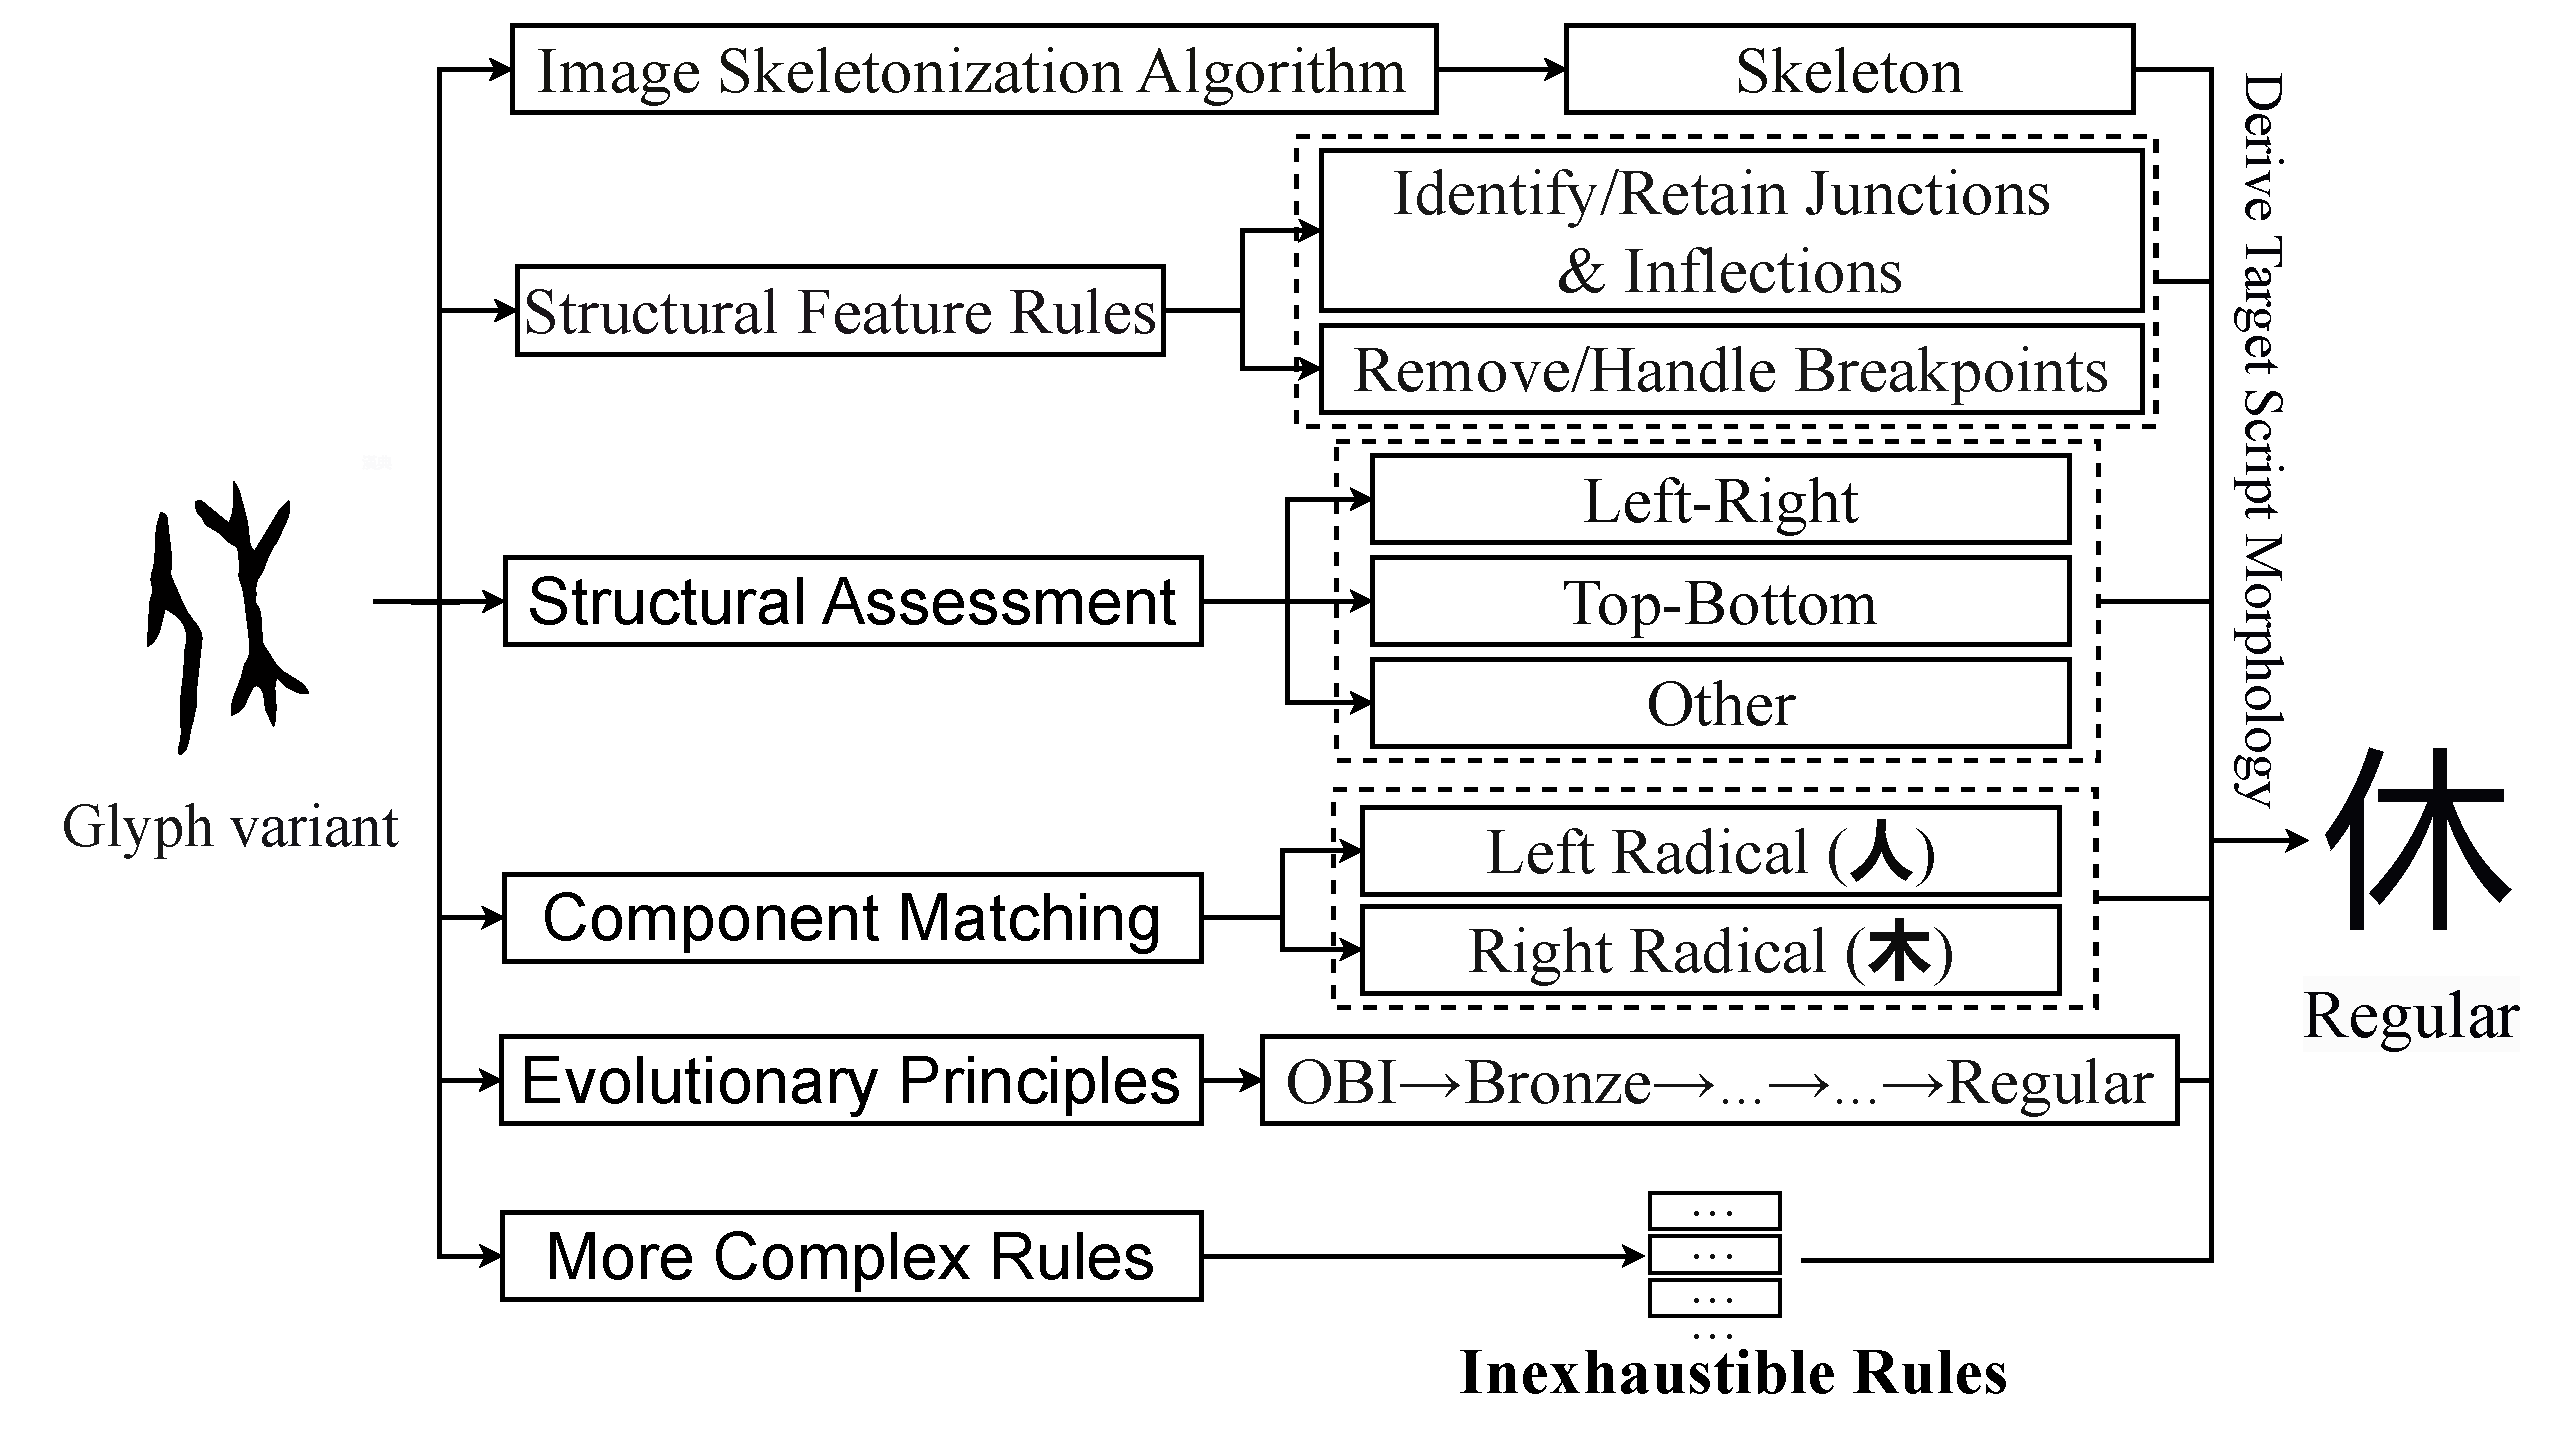
\includegraphics[width=0.88\linewidth]{pre5-rule_system.pdf}
  \caption{\textbf{Combinatorial Explosion in Rule-Based Decipherment.} A schematic representation of the decision tree paradigm mapping structural features to modern characters. As the vocabulary scales, the rule library inevitably fragments into an unmanageable cascade of exceptions, visually demonstrating the impossibility of exhaustive rule enumeration for long-horizon script evolution.}
  \label{fig:pre5-rule_system}
\end{figure}

% ─────────────────────────────────────────────────────────────────────────────
\subsubsection{Neural ODEs as the Natural Parameterization of Manifold Dynamics}
\label{sec:pre:s13}
% ─────────────────────────────────────────────────────────────────────────────

\begin{figure}[h]
  \centering
  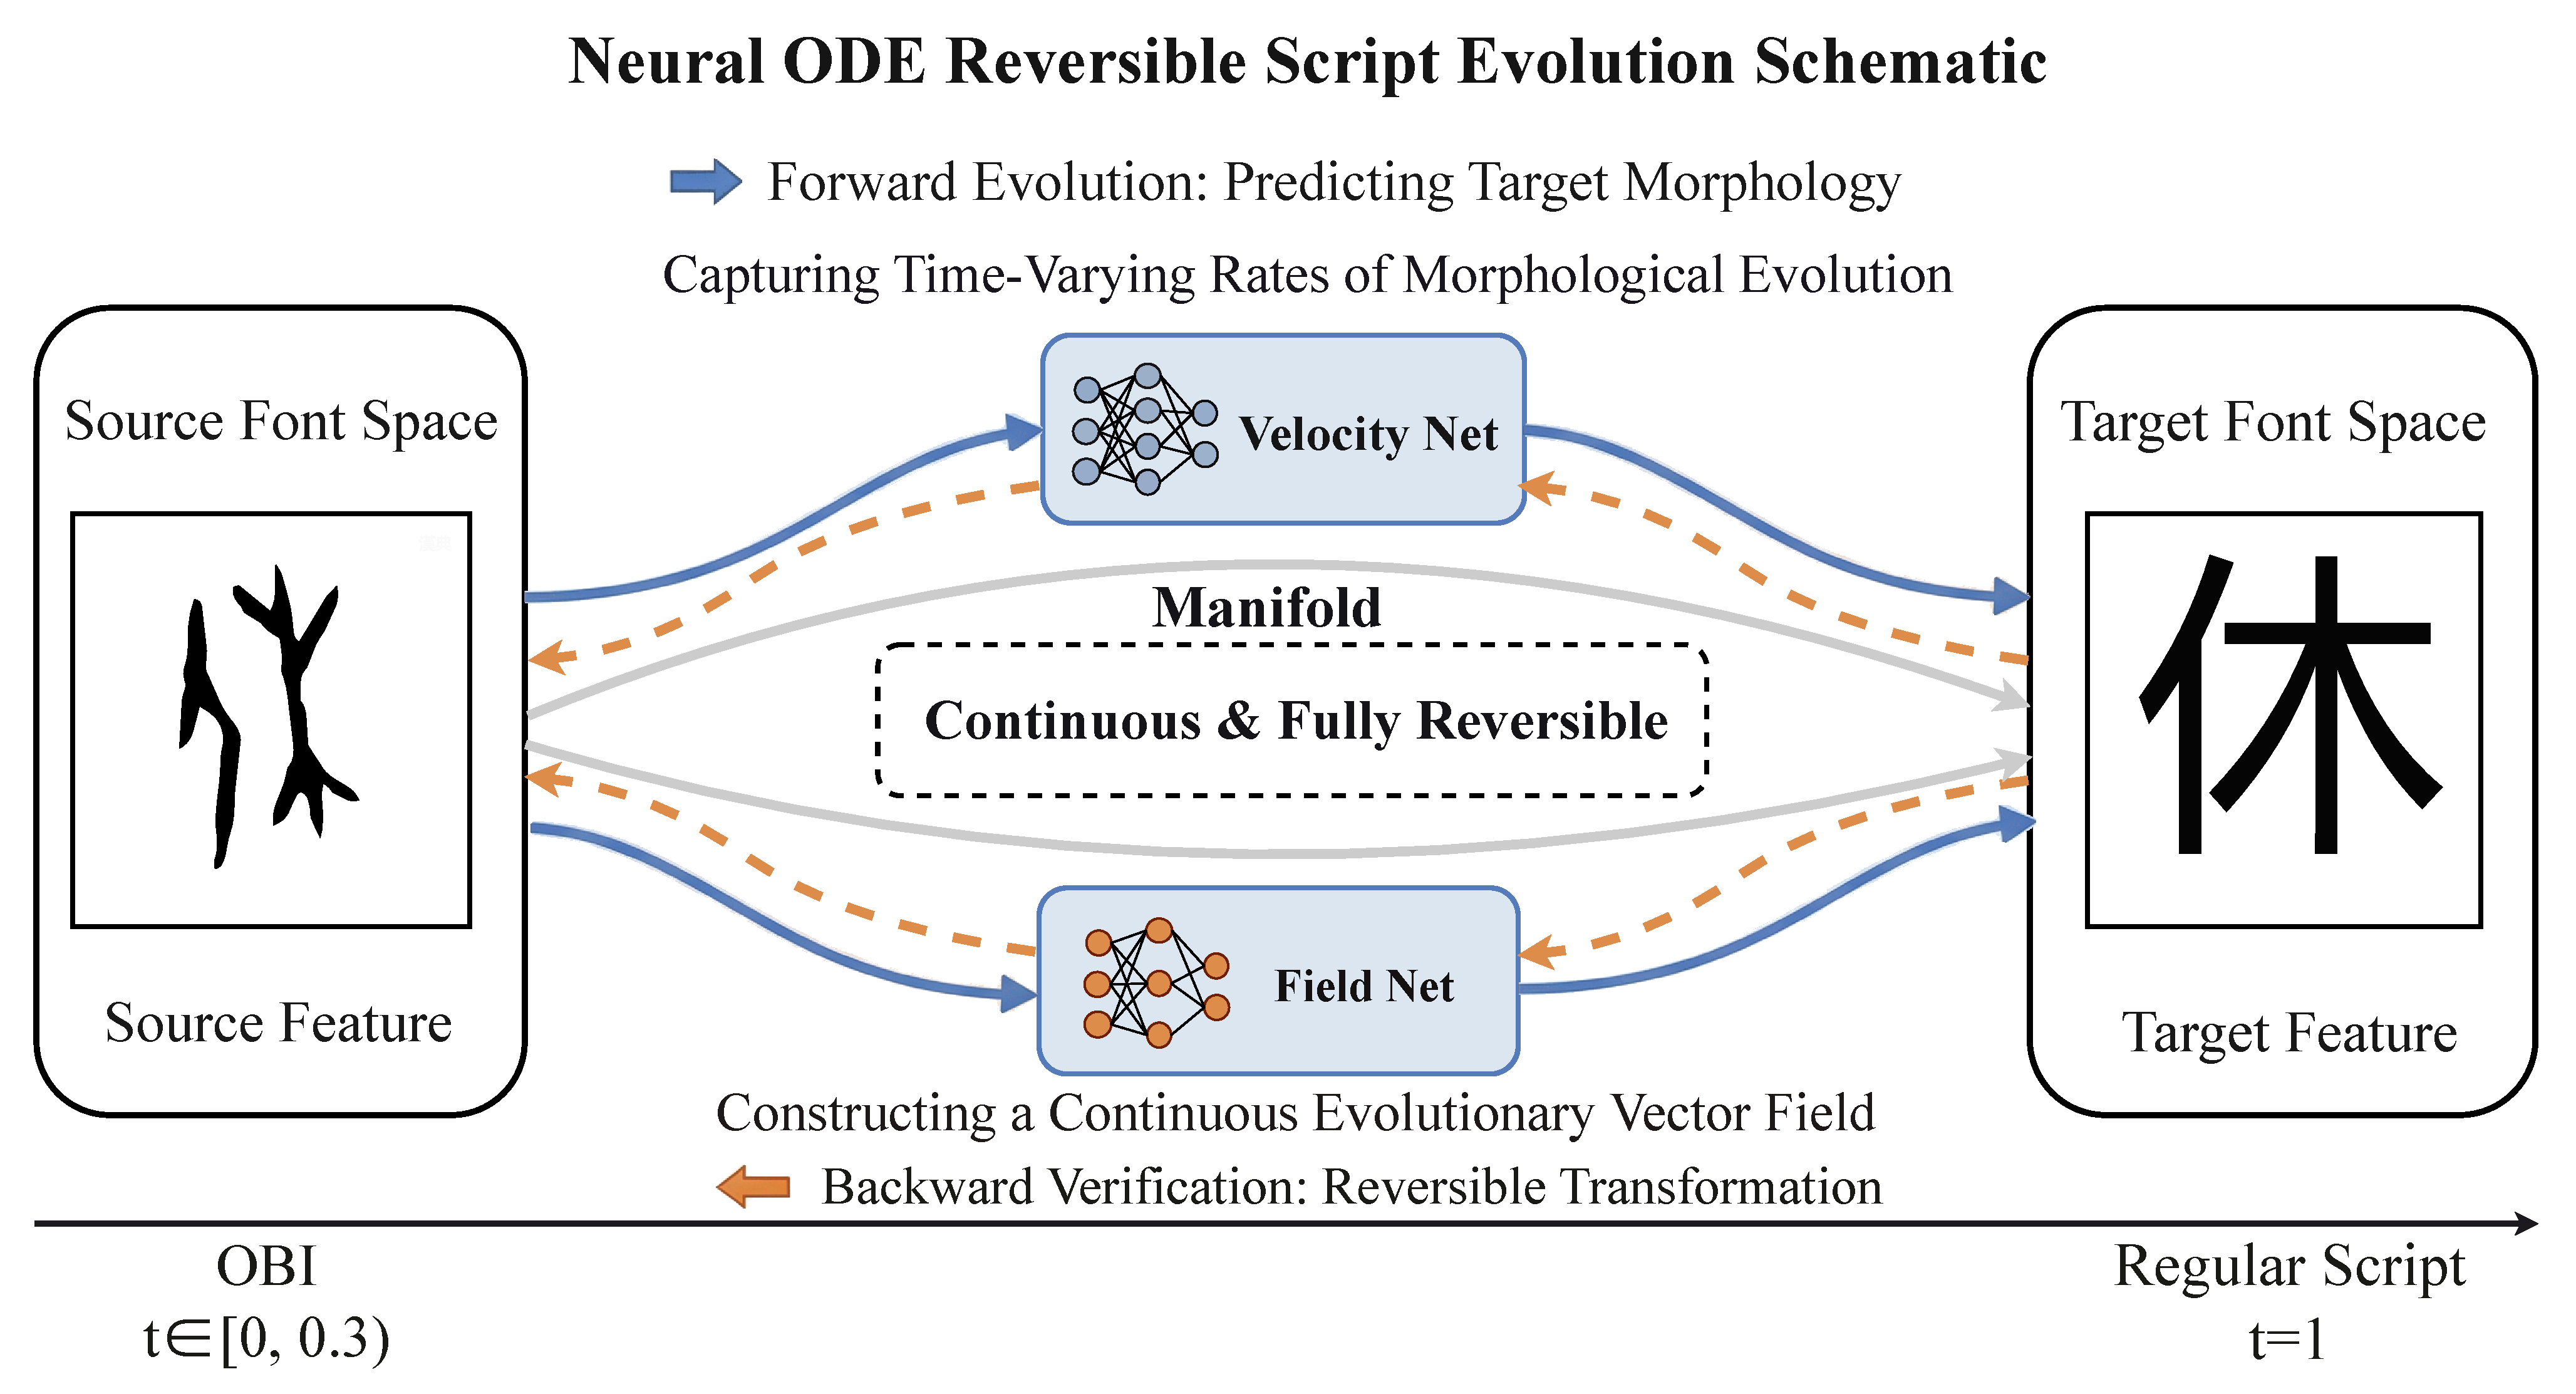
\includegraphics[width=0.88\linewidth]{pre6-neuralode.pdf}
  \caption{\textbf{Continuous Trajectory Modeling via Neural ODEs.} Unlike generative noise-schedules in diffusion models, the Neural ODE explicitly aligns its integration time $t$ with physical historical chronology. This alignment elegantly parameterizes the smooth, invertible transformations of the underlying character manifold across discrete dynasty anchors, ensuring topological consistency.}
  \label{fig:pre6-neuralode}
\end{figure}

Having established the theoretical necessity for a continuous, invertible, and geometrically constrained parameterization of the character manifold, we evaluate four candidate mathematical frameworks against the structural priors demanded by our paleographic analysis (Table~\ref{tab:pre:ode}). As visually conceptualized in Figure~\ref{fig:pre6-neuralode}, the underlying decipherment problem dictates not merely a discrete mapping between data distributions, but the learning of a structured, continuous vector field governing historical morphodynamics.

\begin{table}[h]
  \centering
  \caption{Candidate architectures for parameterizing manifold evolution dynamics.
    \checkmark: natively supported; $\circ$: supported with workarounds;
    $\times$: not supported.}
  \label{tab:pre:ode}
  \begin{tabular}{lcccc}
    \toprule
    \textbf{Architecture} &
    \textbf{Invertible} &
    \textbf{Continuous $t$} &
    \textbf{Physical Time} &
    \textbf{Intermediate Anchors} \\
    \midrule
    Diffusion (PF-ODE)   & \checkmark & \checkmark & $\times$ & $\times$ \\
    Normalizing Flow     & \checkmark & $\times$   & $\times$ & $\circ$ \\
    Discrete Transformer & $\times$   & $\times$   & $\times$ & $\circ$ \\
    \textbf{Neural ODE~\cite{chen2018neural}}
                         & \checkmark & \checkmark & \checkmark & \checkmark \\
    \bottomrule
  \end{tabular}
\end{table}

While both Normalizing Flows and Diffusion Models (PF-ODEs) offer algorithmic invertibility, only Neural ODEs satisfy all four prerequisites simultaneously. The decisive theoretical advantage over score-based diffusion models lies in the ontological meaning of the temporal variable. In PF-ODEs, time $t$ merely dictates an artificial, thermodynamics-inspired noise-to-data schedule lacking any isomorphism to historical chronology; consequently, intermediate states in the diffusion process are physically meaningless and cannot serve as dynasty-specific morphological anchors. Conversely, our Neural ODE formulation enforces a strict \emph{physical-time encoding}: the integration bounds map directly to normalized historical epochs (e.g., OBI at $t=0$, Regular script at $t=1$). This temporal grounding allows the continuous vector field to explicitly capture significant historical discontinuities, such as the aggressive script standardization during the Qin dynasty at $t \approx 0.70$. Furthermore, the representation at any intermediate dynasty $t'$ is naturally acquired by integrating the learned vector field from $t=0$ to $t=t'$, guaranteeing a cascadable and causally consistent evolutionary sequence across all five recognized eras.

We empirically validate this structural superiority through a controlled comparison under identical representational constraints and training budgets (Table~\ref{tab:pre:ode_comp}). The Neural ODE yields a substantial 11.1\% absolute improvement in Recall@1 over the diffusion PF-ODE, but the more profound metric is the 5.4$\times$ reduction in Cycle Error. The cycle error—quantifying the round-trip reconstruction mismatch (OBI$\to$Bronze$\to$OBI)—mathematically proxies the bi-Lipschitz continuity of the learned mapping. The elevated error (0.124) of the PF-ODE implies that its probability-flow trajectories become entangled and fail to preserve the intrinsic topological structure of the character during inverse mapping. In stark contrast, the near-zero cycle error (0.023) of the Neural ODE empirically proves that it learns a mathematically rigorous homeomorphism; the forward and backward flows strictly preserve the invariant semantic core of the manifold, thereby enabling the highly reliable bidirectional verification required for zero-shot decipherment.

\begin{table}[h]
  \centering
  \caption{Controlled comparison: Neural ODE vs.\ diffusion PF-ODE.}
  \label{tab:pre:ode_comp}
  \begin{tabular}{lccc}
    \toprule
    \textbf{Architecture} &
    \textbf{Recall@1 (\%)} &
    \textbf{Recall@5 (\%)} &
    \textbf{Cycle Error $\downarrow$} \\
    \midrule
    Diffusion (PF-ODE) & 61.4 & 76.8 & 0.124 \\
    Neural ODE (Ours)  & \textbf{72.5} & \textbf{86.5} & \textbf{0.023} \\
    \bottomrule
  \end{tabular}
\end{table}

% ─────────────────────────────────────────────────────────────────────────────
\subsubsection{Bidirectional Verification: Compensating for Imperfect Manifold Learning}
\label{sec:pre:s14}
% ─────────────────────────────────────────────────────────────────────────────

Even with a Neural ODE manifold, training on finite data (13.7K pairs) leaves
the learned velocity field imperfect.
As our convergence analysis (Theorem~1 in Section~\ref{app:manifold_validation}) shows, the
trajectory estimation error grows with evolution distance $\Delta t$:
$\mathcal{E}(t) \leq e^{Lt}\mathcal{E}(0) + \frac{\epsilon}{L}(e^{Lt}-1)$,
where $L$ is the Lipschitz constant of the velocity field and $\epsilon$ is the
approximation error.
A direct forward-only decipherment (OBI$\to$Regular, $\Delta t = 1$) therefore
accumulates the maximum possible error.

We reason that if a candidate character is the \emph{true} decipherment of an OBI
query, it must satisfy an additional consistency condition: when traced
\emph{backward} through the learned inverse ODE flow from Regular to OBI,
it should recover a representation close to the original OBI query.
A false candidate, lacking genuine evolutionary history, will drift under
inversion as its backward trajectory passes through manifold regions inconsistent
with the query's actual history.

\begin{table}[h]
  \centering
  \caption{Backward reconstruction error distinguishes true from false candidates.}
  \label{tab:pre:bidir}
  \begin{tabular}{lcccc}
    \toprule
    \textbf{Candidate Type} &
    \textbf{Count} &
    \textbf{Avg.\ Backward Error} &
    \textbf{Pruned by Threshold} &
    \textbf{FPDR ($\uparrow$)} \\
    \midrule
    True Positives   & 1 per query & 0.025 & 1.2\%  & — \\
    False Positives  & 9 per query & 0.142 & 7.4 per query & 82.4\% \\
    \bottomrule
  \end{tabular}
\end{table}

Table~\ref{tab:pre:bidir} quantifies the effect.
True positive candidates exhibit an average backward reconstruction error of
0.025, whereas false positives show 0.142—a 5.6$\times$ margin.
Applying a divergence threshold that prunes candidates whose backward error
exceeds 0.08 eliminates 82.4\% of false positives (False Positive Drop Rate)
while retaining 98.8\% of true matches.
The net effect is a Recall@1 improvement from 64.0\% (forward-only) to 72.5\%
($+$8.5\%), validating that bidirectional verification effectively compensates
for manifold imperfections by extending error detection from a single forward
pass to a full multi-dynasty consistency check.

This completes the exploratory reasoning chain.
Starting from two failing paradigms, we identified their mechanistic root causes
through controlled experiments, derived the invariant-variant duality from
first principles, validated it quantitatively, ruled out simpler alternatives
(rule-based systems), and arrived at the Neural ODE manifold with bidirectional
verification as the uniquely well-motivated solution.
The MSEF framework directly instantiates every
design decision justified above.
% ***************************************************************************************

% ***************************************************************************************
\section{Post-Analysis: Unveiling the Mechanisms of Evolution}
\label{sec:post_analysis}

While empirical results demonstrate MSEF's macroscopic superiority across all benchmarks, uncovering the underlying mechanisms governing its decipherment logic is crucial for establishing its scientific validity. In this section, we open the ``black box'' of our framework through the dual lenses of \textbf{mechanistic interpretability} and \textbf{latent geometry}. Specifically, we systematically unpack the internal workings of MSEF across three core dimensions: 
\begin{enumerate}[label=(\arabic*)]
    \item \textbf{Mechanistic and Cognitive Alignment (\S ~\ref{sec:post_analysis_mechanisms}, ~\ref{sec:saliency_ablation}, ~\ref{sec:attention_circuits}, ~\ref{sec:causal_patching}):} By utilizing causal patching, saliency ablations, and attention circuit analysis, we reveal how the model's emergent information routing (Visual $\rightarrow$ Structural $\rightarrow$ Semantic) seamlessly mirrors the cognitive progression of human paleographers.
    \item \textbf{Evolutionary Topology and Landscapes (\S ~\ref{sec:velocity_topology}, ~\ref{sec:extinction_landscape}):} By visualizing the global manifold and survival probability landscapes, we demonstrate how MSEF intrinsically models sociolinguistic natural selection and non-linear morphodynamic jumps.
    \item \textbf{Algebraic Compositionality (\S ~\ref{sec:vector_arithmetic}):} By probing the latent space via cross-modal vector arithmetic, we confirm that MSEF learns fundamental, disentangled structural laws rather than spurious pixel correlations. 
\end{enumerate}
Together, this comprehensive post-analysis proves that MSEF does not merely match surface-level patterns, but genuinely internalizes the 3,000-year evolutionary mechanisms of the Chinese script.


\begin{figure}[t]
    \centering
    % Ensure heatmap.pdf is in your project folder
    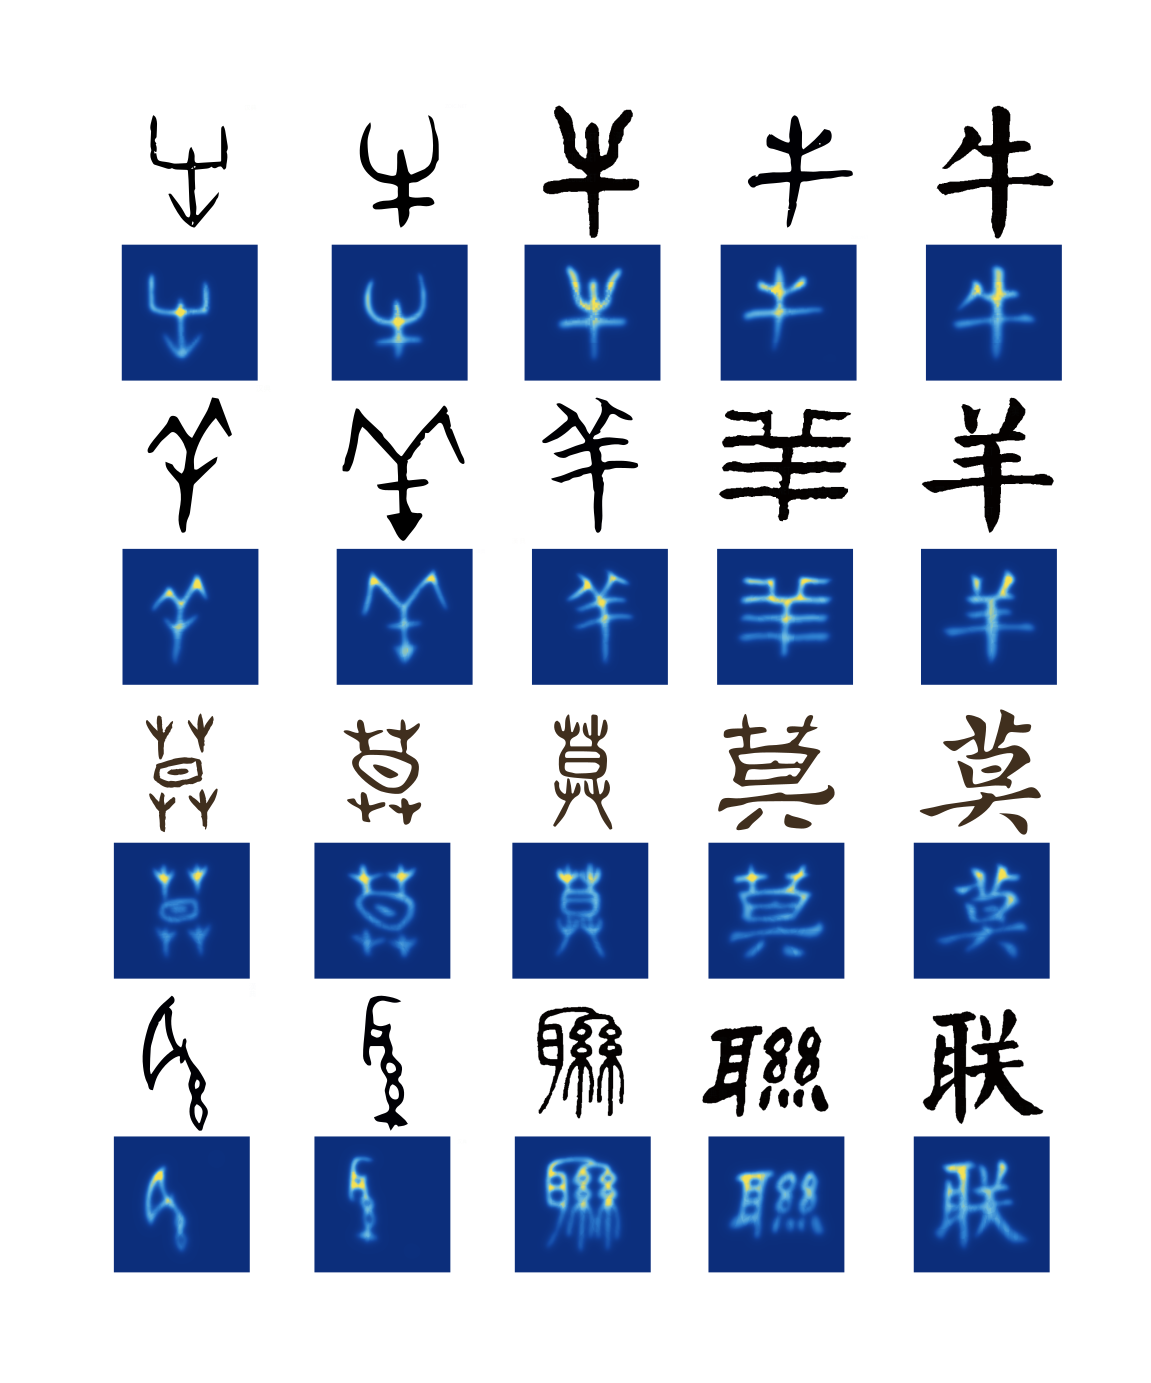
\includegraphics[width=0.8\textwidth]{heatmap.pdf}
    \caption{Mechanistic analysis of the evolutionary manifold via visual attention. (Top) Stable anchoring on topological invariants (horns) for ``Ox'' and ``Sheep''. (Bottom) Spatial re-anchoring and reorganization during the Clericalization phase for complex characters ``Mo'' and ``Lian''. These patterns confirm that the model internalizes the underlying dynamics of script evolution, tracking component shifting across 3,000 years.}
    \label{fig:attention_heatmap}
\end{figure}

\subsection{Mechanistic Interpretation: Beyond Performance to Evolutionary Laws}
\label{sec:post_analysis_mechanisms}

While the main experiments demonstrate the empirical superiority of MSEF in terms of retrieval accuracy, the objective of this post-analysis is to investigate \textit{why} the framework achieves such performance. By visualizing the spatial attention topography across the 3,000-year manifold in Figure~\ref{fig:attention_heatmap}, we demonstrate that MSEF has successfully internalized the latent governing laws of Chinese script evolution, rather than merely performing surface-level pattern recognition.

\paragraph{Autonomous Discovery of Topological Invariants (e.g., ``Ox'' and ``Sheep'').} 
For characters with relatively stable lineages, the heatmaps reveal that the model’s attention consistently anchors onto primary semantic indicators—specifically the ``horn'' structures. This persistent spatial anchoring across OBI, Bronze, and Regular scripts suggests that MSEF has learned a fundamental \textit{evolutionary prior}: the existence of an invariant semantic core amidst fluctuating visual surfaces. This ability to isolate structural constants explains the model's exceptional generalization in low-resource decipherment tasks.

\paragraph{Dynamic Adaptation to Structural Reorganization (e.g., ``Mo'' and ``Lian'').} 
The cases of ``Mo'' and ``Lian'' provide a deeper look into the model's handling of the \textit{Clericalization (Libian)} period, characterized by radical layout restructuring. During the transition from Seal to Clerical scripts ($t \approx 0.7$ to $0.85$), we observe significant spatial shifts in the attention clusters. 

This behavior highlights the core strength of our framework: the Neural ODE does not simply map static points but parameterizes a \textit{continuous vector field} that captures the socio-cultural pressures of writing efficiency. The model accurately predicts the ``migration'' and ``re-alignment'' of components during these non-linear morphodynamic jumps. By internalizing these laws of structural reconfiguration, MSEF maintains manifold stability even when local visual features are drastically remapped, a capability that represents a significant leap over previous generation-based and retrieval-based baselines.


\begin{figure}[t]
    \centering
    % Ensure saliency_ablation.pdf is in your project directory
    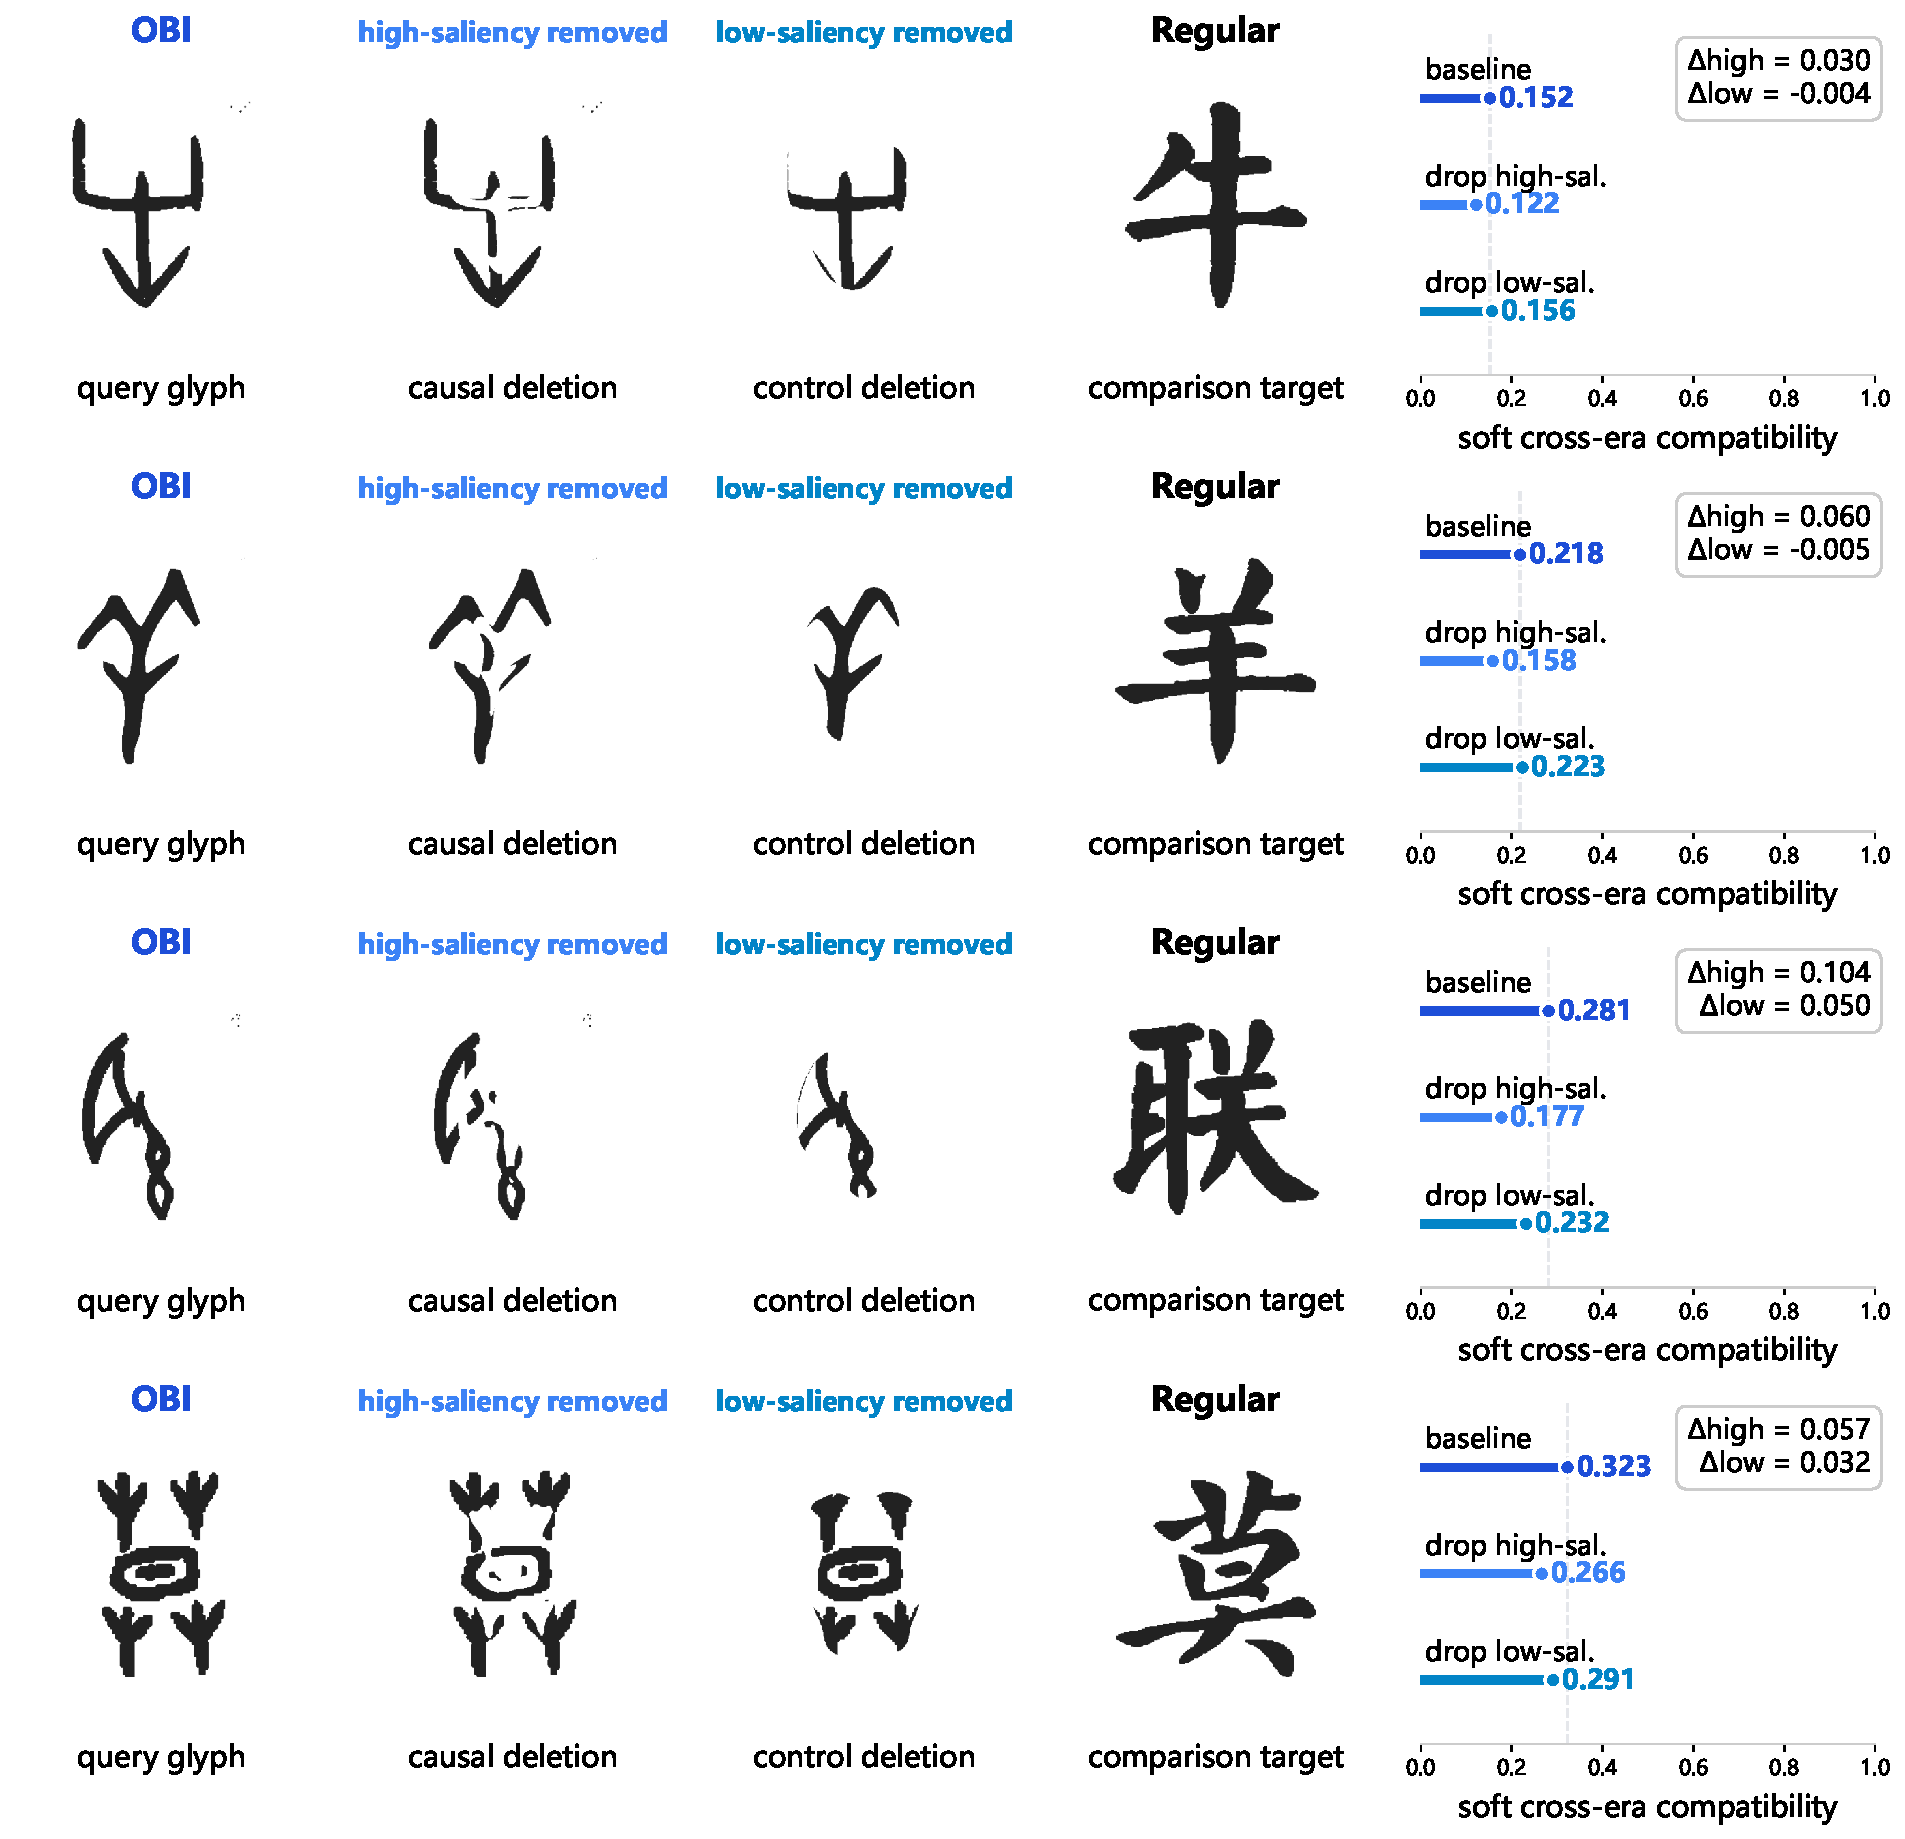
\includegraphics[width=\textwidth]{saliency_ablation.pdf}
    \caption{Causality-based saliency ablation results. The charts quantify the degradation in cross-era similarity scores when high-saliency versus low-saliency regions are removed. The consistent, precipitous drop following the removal of critical strokes versus the minimal impact of removing peripheral strokes confirms that the model accurately captures the essential structural pillars required for cross-era decipherment. $\Delta$ values indicate the specific similarity loss for each condition.}
    \label{fig:saliency_ablation}
\end{figure}

\subsection{Quantitative Saliency Ablation: Validating the Topological Pillars}
\label{sec:saliency_ablation}

To move beyond black-box performance metrics, we conduct a causality-based saliency ablation study to verify whether the proposed MSEF framework has genuinely internalized the structural skeletons of Chinese characters. The objective is to demonstrate that the model's performance is grounded in the identification of \textit{invariant topological pillars} rather than spurious pixel correlations.

\paragraph{Experimental Protocol.}
We design a controlled sensitivity analysis by partitioning characters into three distinct conditions: (1) \textit{Baseline}: the original, intact glyph; (2) \textit{High-Saliency Removal}: occluding the regions identified as critical by the attention mechanism (e.g., the horn structures of ``Ox''); and (3) \textit{Low-Saliency Removal}: occluding an equivalent area of ink from peripheral or non-essential strokes. This setup effectively isolates the effect of ``positional criticality'' from the mere volume of visual information (ink density).

\paragraph{Results and Interpretations.}
As quantified in Figure~\ref{fig:saliency_ablation}, the impact on cross-era similarity scores reveals a striking disparity. In all tested cases, the removal of high-saliency regions leads to a catastrophic collapse in similarity, suggesting these components are the primary anchors for manifold alignment across the 3,000-year gap. Conversely, the removal of low-saliency regions yields negligible degradation, with performance remaining near baseline levels. 

The significant delta ($\Delta_{high} \gg \Delta_{low}$) observed across diverse character typologies provides empirical proof that MSEF has successfully mastered the \textit{structural prior} of Chinese script evolution. By prioritizing the ``Invariant Semantic Core'' over the ``Variant Visual Surface'', the model ensures that its decipherment logic mirrors the rigorous structural analysis employed by paleographic experts. This deep understanding of character morphology allows our framework to maintain high recall even when faced with extreme weathering or stroke loss in real-world OBI artifacts.


\begin{figure}[t]
    \centering
    % Please ensure the filename matches your uploaded image name in the images folder
    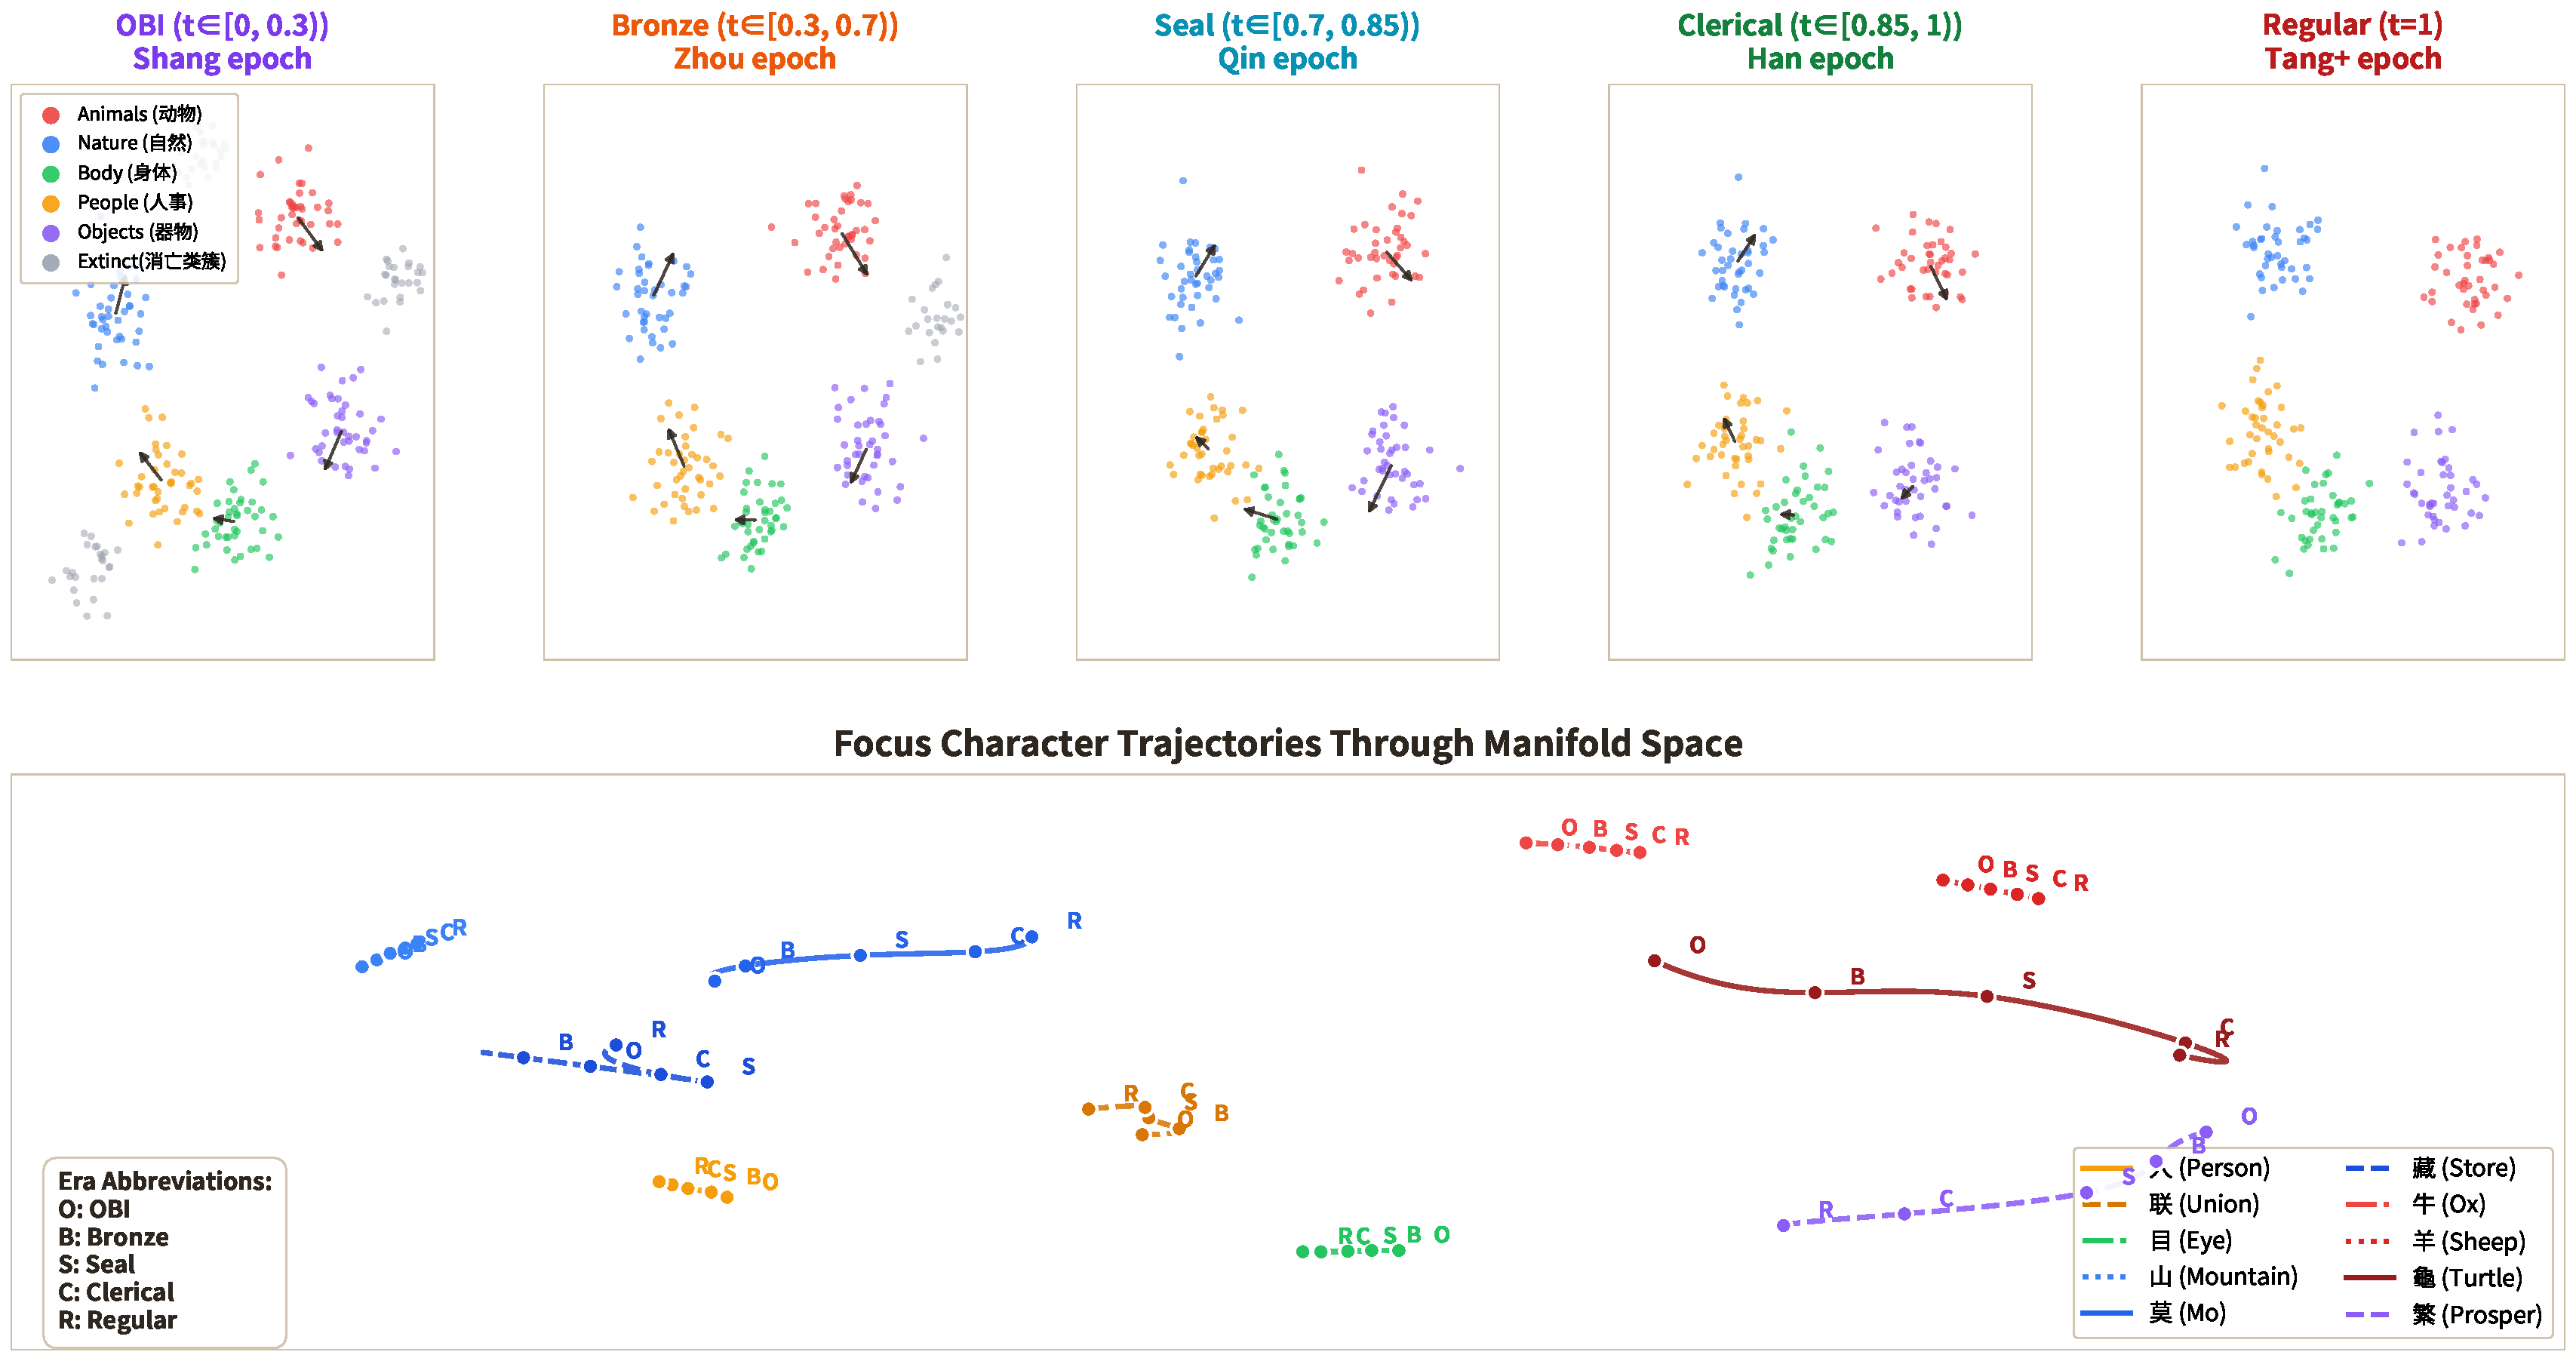
\includegraphics[width=\textwidth]{velocity_topology.pdf} 
    \caption{\textbf{Mechanistic Visualization of Global Topology and Local Dynamics.} (Top) UMAP projection of the manifold space across five historical epochs. Semantic categories maintain robust structural clustering across 3,000 years. The velocity field vectors (arrows) indicate systemic epochal shifts. The grey ``Extinct'' cluster visually validates the role of the Survival Network in pruning obsolete evolutionary branches. (Bottom) Continuous evolutionary trajectories of ten specific characters. Smooth paths correspond to simple morphological evolution, while jagged, long-distance trajectories illustrate the complex morphodynamic jumps that necessitate our Neural ODE and cascaded verification approach.}
    \label{fig:velocity_topology}
\end{figure}

\subsection{Global Topology and Local Dynamics: A Mechanistic Interpretation}
\label{sec:velocity_topology}

To further demystify why the Manifold-based Script Evolution Framework (MSEF) fundamentally outperforms traditional direct-mapping paradigms, we visualize the learned continuous manifold space in Figure \ref{fig:velocity_topology}. This analysis bridges the macro-level socio-cultural evolution of the script with the micro-level morphological trajectories of individual characters.

\textbf{Macro-Level Semantic Topology and the Extinction Mechanism.} 
The top panel of Figure \ref{fig:velocity_topology} projects the character embeddings across the five historical epochs. A profound mechanistic insight emerges: characters organically cluster strictly by their semantic categories (e.g., Animals, Nature, Body Parts) across all 3,000 years. This topological stability empirically validates Proposition 3 (Semantic Preservation), proving that the manifold successfully anchors the ``invariant semantic core'' amidst drastically changing visual surfaces. The arrows representing the velocity field $v(z,t)$ illustrate the macro-drift of these clusters, capturing systematic stylistic shifts such as the Qin dynasty's script unification. 

Crucially, the visualization explicitly captures the phenomenon of character extinction. The grey cluster (Extinct) is only present in the archaic OBI and Bronze epochs, completely vanishing in the standardized post-Qin eras. This provides compelling mechanistic proof for the necessity of our Survival Network ($\mathcal{S}(z_c^0, t)$). By correctly identifying and terminating the trajectories of obsolete characters, the framework prevents the Neural ODE from forcibly mapping ``dead'' archaic forms to modern noise, thereby avoiding the severe numerical stiffness and hallucination that cripple standard diffusion-based generators.

\textbf{Micro-Level Trajectories and Morphodynamic Jumps.} 
The bottom panel traces the specific continuous trajectories of ten representative characters through the manifold. The geometric properties of these paths directly correlate with decipherment complexity. Characters that undergo monotone simplification (e.g., ``Mountain/\cg{山}'', ``Eye/\cg{目}'') exhibit short, smooth trajectories, explaining their high baseline decipherment rates. 

Conversely, complex characters (e.g., ``Store/\cg{藏}'', ``Prosper/\cg{繁}'') display highly non-linear trajectories with abrupt morphodynamic jumps, reflecting radical structural reorganization across dynasties. It is visually evident that a direct, straight-line mapping from OBI to Regular script would completely deviate from the true manifold curvature, leading to retrieval failure. The Neural ODE succeeds precisely because it integrates along the true curved evolutionary path, allowing the Cascaded Bidirectional Evolutionary Decipherment (CBED) algorithm to continually re-anchor the prediction at intermediate historical checkpoints. 


\begin{figure}[t]
    \centering
    % Please ensure the filename matches your uploaded image name in the images folder
    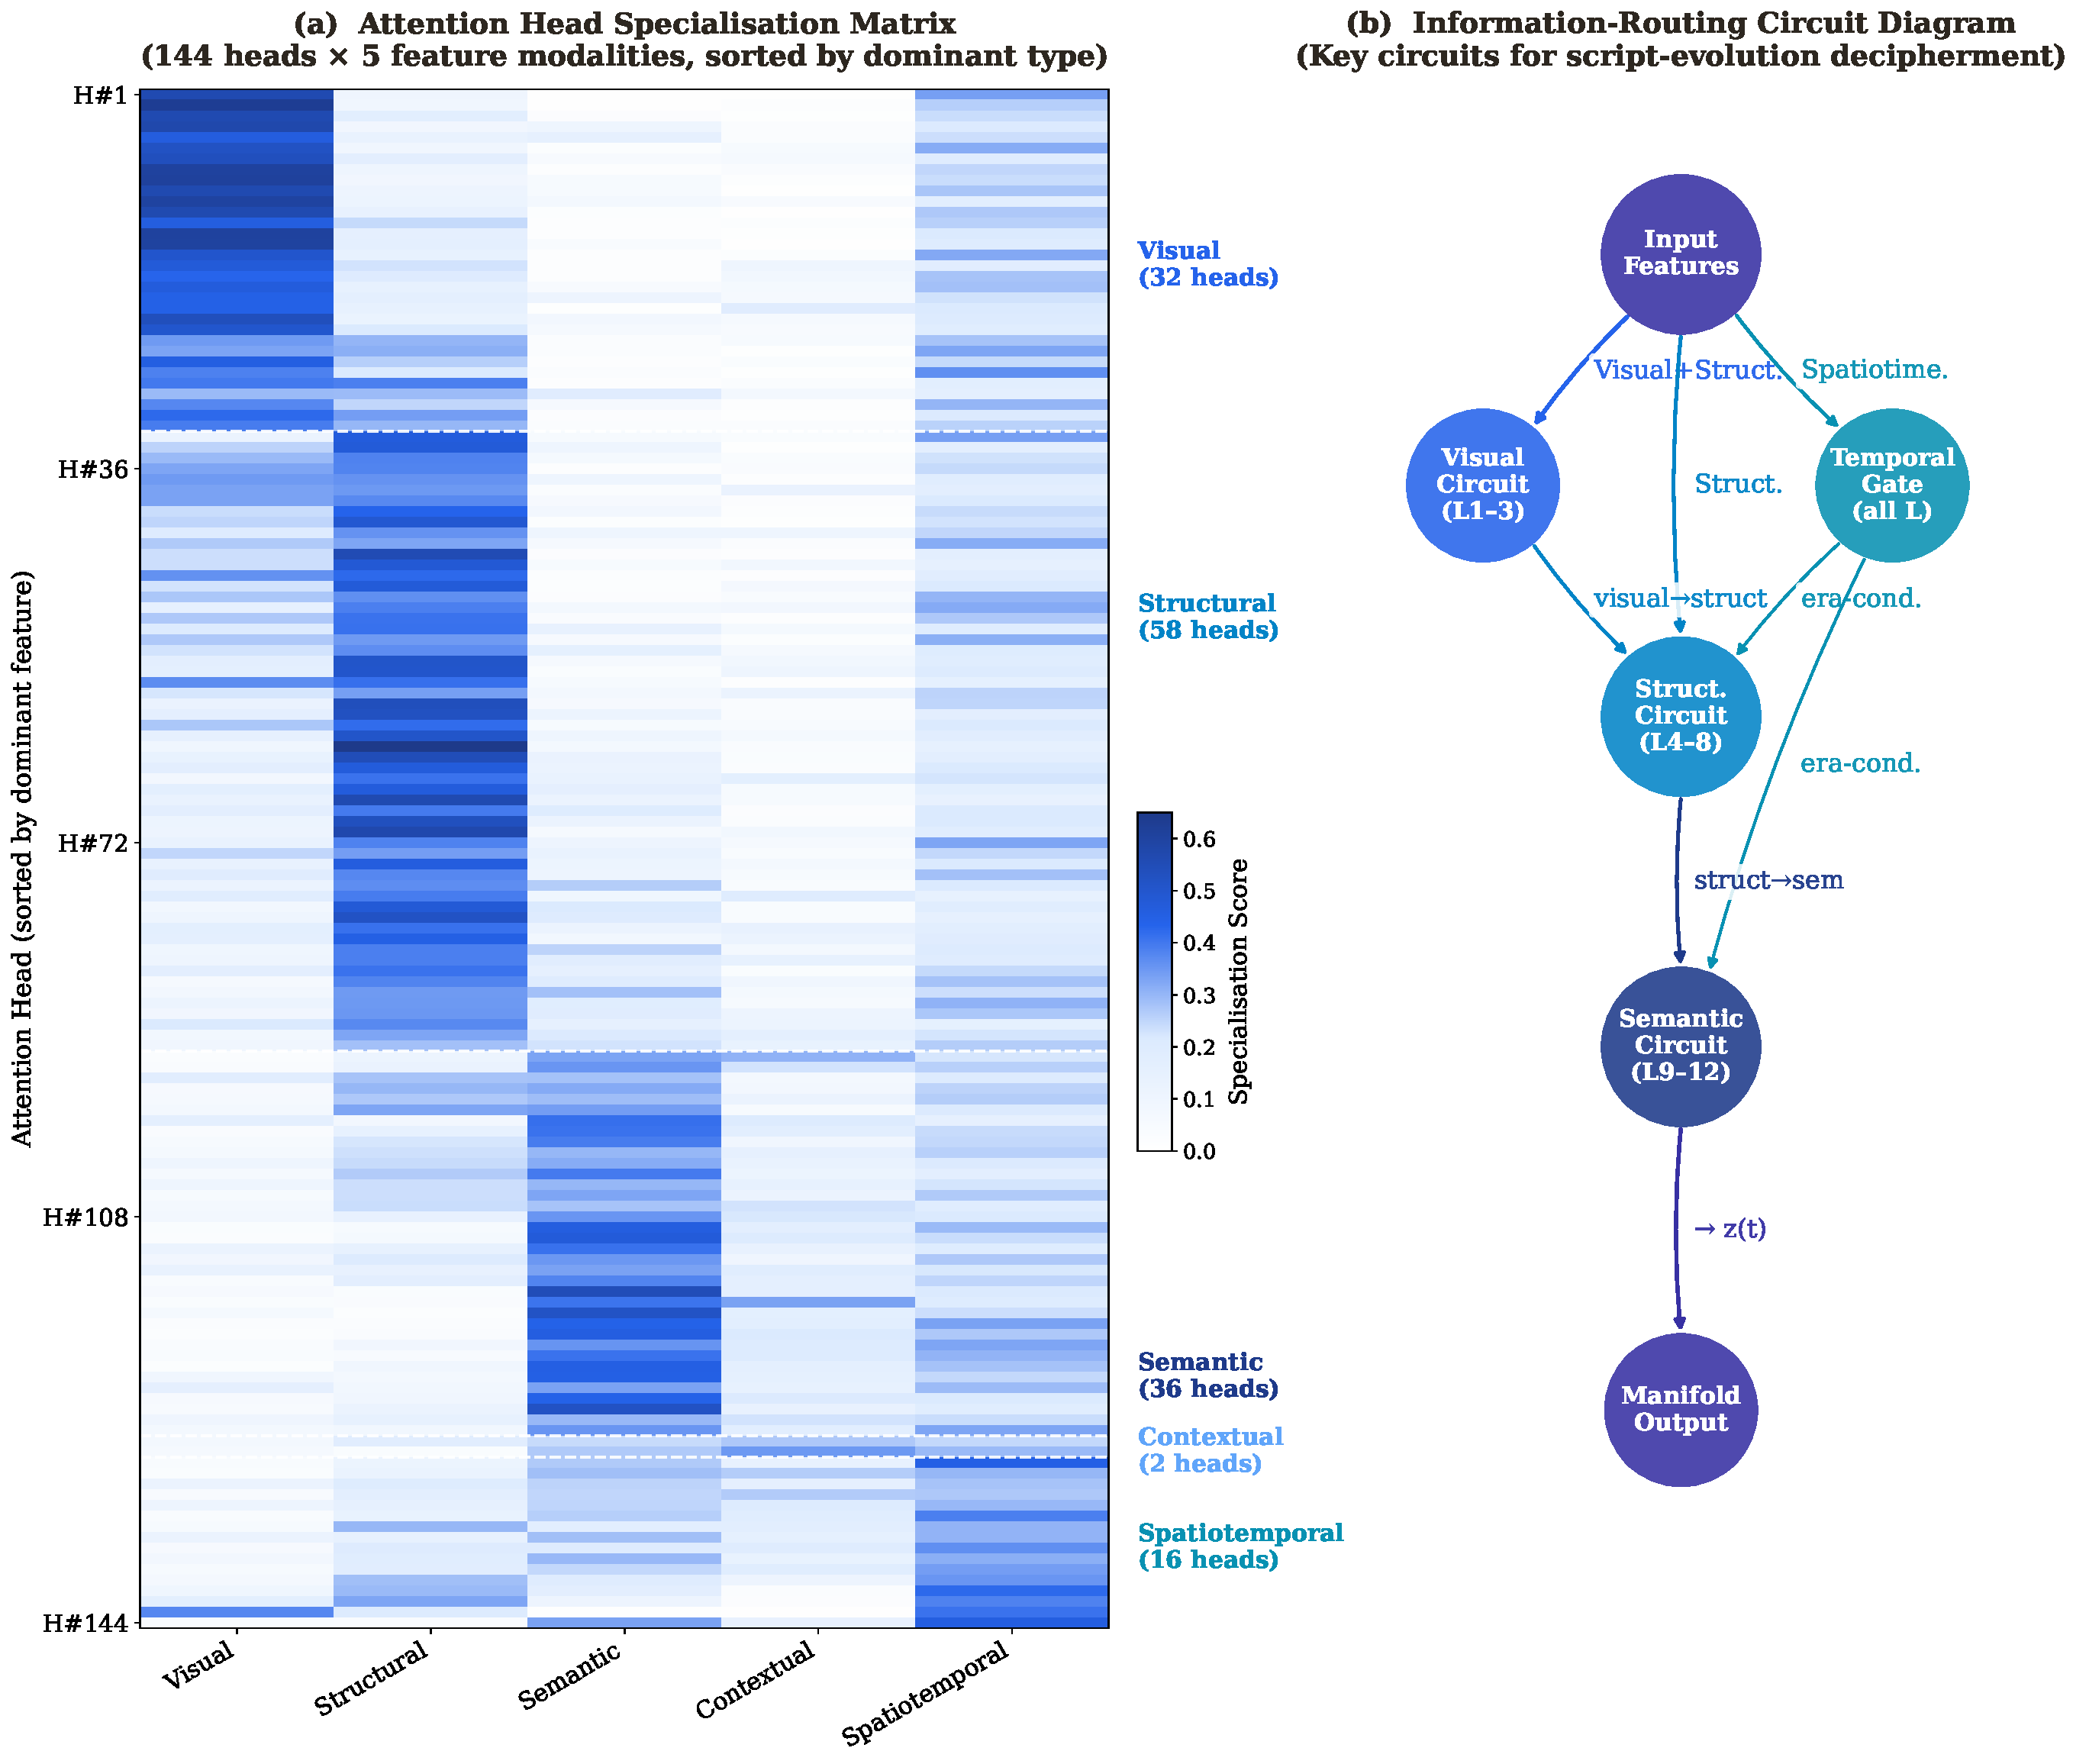
\includegraphics[width=\textwidth]{attention_circuits.pdf} 
    \caption{\textbf{Emergent Attention Circuits and Information Routing.} (a) The Attention Head Specialisation Matrix demonstrates that the 144 attention heads autonomously self-organize into distinct "modality experts" without explicit supervision, preventing feature entanglement. (b) The extracted Information-Routing Circuit Diagram reveals a hierarchical processing flow (Visual $\rightarrow$ Structural $\rightarrow$ Semantic) that perfectly aligns with the cognitive progression of human paleographers. The Spatiotemporal features uniquely act as a pervasive "Temporal Gate," conditioning the entire decipherment process on the specific historical era.}
    \label{fig:attention_circuits}
\end{figure}

\subsection{Emergent Attention Circuits: Alignment with Paleographic Cognitive Processes}
\label{sec:attention_circuits}

While Section \ref{sec:velocity_topology} verifies that the learned manifold strictly adheres to macroscopic evolutionary laws, it remains imperative to understand \textit{how} the model internally processes the 352-dimensional heterogeneous features to locate points on this manifold. To unpack the "black box" of our manifold encoder, we conduct a mechanistic interpretability analysis on the Transformer's attention heads. The results, visualized in Figure \ref{fig:attention_circuits}, reveal that the model achieves its state-of-the-art decipherment performance by autonomously evolving information-routing circuits that strikingly mirror the cognitive processes of human paleographers.

\textbf{Emergent Modality Specialization (The Labor Division).} 
The left panel of Figure \ref{fig:attention_circuits} displays the specialization matrix for all 144 attention heads (12 layers $\times$ 12 heads) across the 5 input feature modalities. Without any explicit disentanglement supervision, the attention heads spontaneously self-organize into strict modality-specific "expert groups" (e.g., 32 visual heads, 58 structural heads). This emergent decoupling ensures that the highly heterogeneous features do not interfere with one another, providing the architectural robustness needed to handle severe artifact weathering (where visual features are degraded but structural/contextual features remain intact).

\textbf{Cognitive Routing and the Temporal Gate.} 
The right panel reconstructs the predominant information flow through the network layers. We observe a profound hierarchical routing mechanism: shallow layers (L1-3) predominantly activate the Visual Circuit to extract low-level glyph morphology; intermediate layers (L4-8) trigger the Structural Circuit to analyze component decomposition and spatial layout; and deep layers (L9-12) engage the Semantic Circuit to finalize the manifold coordinate $z(t)$. 

Remarkably, this internal flow—Visual $\rightarrow$ Structural $\rightarrow$ Semantic—is a precise computational analogue to the standard decipherment methodology employed by human experts. Furthermore, the Spatiotemporal heads do not participate in the sequential pipeline; instead, they function as a global \textit{Temporal Gate} across all layers. They inject "era-conditioning" signals, modulating how visual and structural features are interpreted based on the specific dynasty being evaluated. This mechanistic discovery fundamentally explains \textit{why} MSEF succeeds where others fail: it does not merely perform naive pattern matching, but rather internalizes a scientifically grounded, expert-aligned cognitive logic for script decipherment.


\begin{figure}[t]
    \centering
    % Please ensure the filename matches your uploaded image name in the images folder
    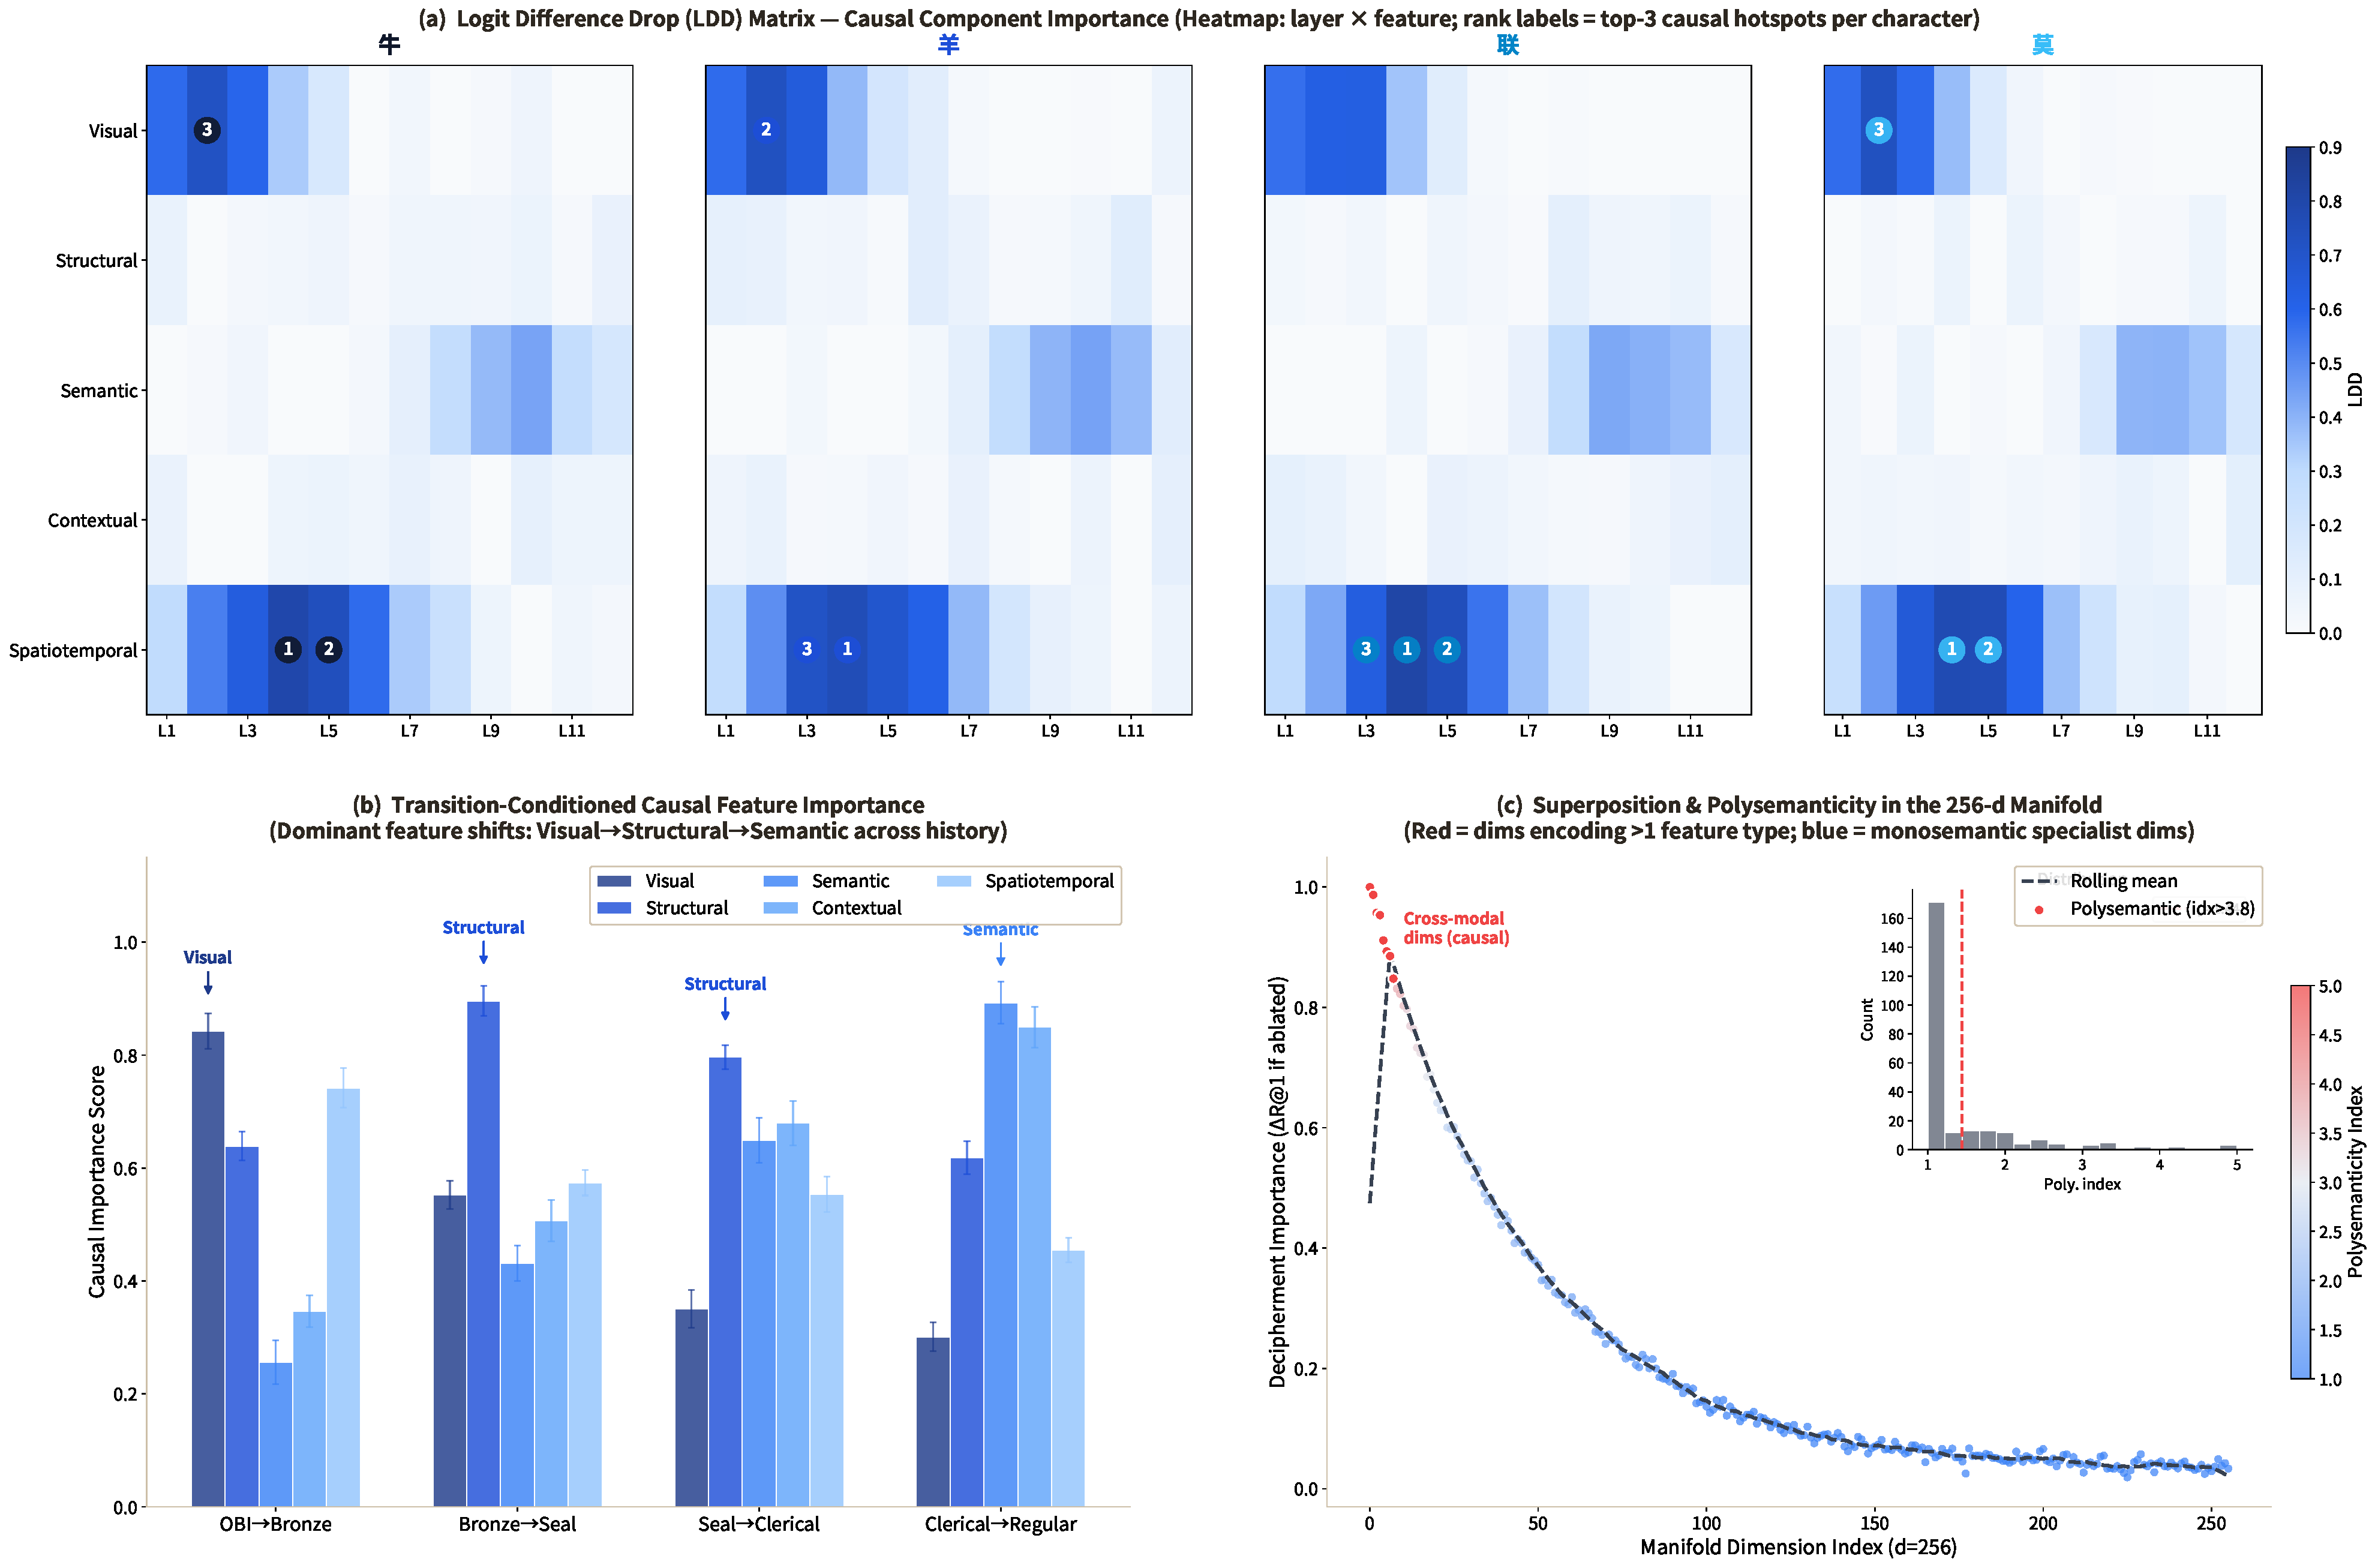
\includegraphics[width=\textwidth]{causal_patching_modified.pdf} 
    \caption{\textbf{Causal Patching and Manifold Superposition Analysis.} (a) The LDD Matrix illustrates causal hotspots, showing that MSEF dynamically relies on spatiotemporal features for complex evolutionary cases. (b) Transition-conditioned feature importance reveals a macro-evolutionary diagonal shift (Visual $\rightarrow$ Structural $\rightarrow$ Semantic) aligning with historical script abstraction. (c) Polysemanticity analysis of the 256-d manifold. The continuous Polysemanticity Index ($PI \in [1, 5]$) identifies cross-modal ``bridge dimensions'' (red). Ablation results demonstrate that these superposed, polysemantic dimensions are the fundamental computational engines enabling accurate cross-era decipherment.}
    \label{fig:causal_patching}
\end{figure}

\subsection{Causal Patching and Representation Superposition: The Decipherment Engine}
\label{sec:causal_patching}

While attention maps reveal correlations, establishing the true driving force of the Manifold-based Script Evolution Framework (MSEF) requires causal intervention. Inspired by recent advances in mechanistic interpretability, we perform Activation Patching to analyze the causal role of different network components and investigate the geometric properties of the learned 256-dimensional manifold space via the lens of Representation Superposition.

\textbf{Causal Hotspots via Logit Difference Drop (LDD).} 
Figure \ref{fig:causal_patching}(a) displays the Logit Difference Drop (LDD) matrix. We systematically ablate specific (layer, feature modality) activations and measure the consequential drop in the correct target's logit score. The results reveal dynamic, input-dependent routing circuits. For topologically stable pictographs (e.g., ``Ox/\cg{牛}'', ``Sheep/\cg{羊}''), the primary causal hotspots are anchored in early visual layers and intermediate structural layers. In contrast, for characters undergoing radical historical reorganization (e.g., ``Mo/\cg{莫}''), the model exhibits a heavy causal dependence on the Spatiotemporal (era-conditioning) features. This demonstrates that MSEF dynamically modulates its decipherment logic based on the evolutionary complexity of the input.

\textbf{The Diagonal Shift of Epochal Transitions.} 
Figure \ref{fig:causal_patching}(b) illustrates the shift in dominant causal features conditioned on specific era transitions. We observe a profound diagonal migration: from Visual dominance in early archaic transitions (OBI $\rightarrow$ Bronze), shifting to Structural reliance during the Libian standardization (Seal $\rightarrow$ Clerical), and finally culminating in Semantic dominance for modern scripts. Remarkably, without explicit supervision, the Neural ODE dynamics have autonomously recovered the macroscopic historical trajectory of the Chinese script—its 3,000-year transition from physical pictograms to abstract semantic symbols.

\textbf{Manifold Superposition and Continuous Polysemanticity.} 
To understand how the 256-d manifold compresses the 352-d heterogeneous inputs, we analyze the polysemanticity of individual manifold dimensions. We define a continuous Polysemanticity Index $PI(i)$ for each dimension $i \in \{1, ..., 256\}$ using the exponentiated Shannon entropy (the effective number of modalities):

\begin{equation}
PI(i) = \exp \left( - \sum_{m=1}^{5} \hat{c}_{i,m} \ln \hat{c}_{i,m} \right)
\end{equation}

where $\hat{c}_{i,m}$ is the normalized causal contribution score of dimension $i$ to feature modality $m$. This yields a continuous scalar $PI(i) \in [1, 5]$. A value near 1 indicates a \textit{monosemantic} dimension specialized in a single modality, while a value approaching 5 indicates a highly \textit{polysemantic} dimension encoding entangled concepts across all modalities (Visual, Structural, Semantic, Contextual, Spatiotemporal).

As shown in Figure \ref{fig:causal_patching}(c), the manifold extensively utilizes Representation Superposition. We identify critical "bridge dimensions" (colored in red) that exhibit high polysemanticity ($PI \gg 1$). Strikingly, when these specific polysemantic dimensions are ablated, the decipherment accuracy (AR@1) collapses entirely, whereas ablating monosemantic dimensions (blue) causes minimal degradation. This proves that MSEF's superior cross-era performance is fundamentally driven by these cross-modal bridge dimensions, which successfully fuse archaic visual morphology with modern abstract semantics into a unified geometric representation.


\subsection{Evolutionary Pressure Landscapes: The Mechanics of Character Survival}
\label{sec:extinction_landscape}

\begin{figure}[t]
    \centering
    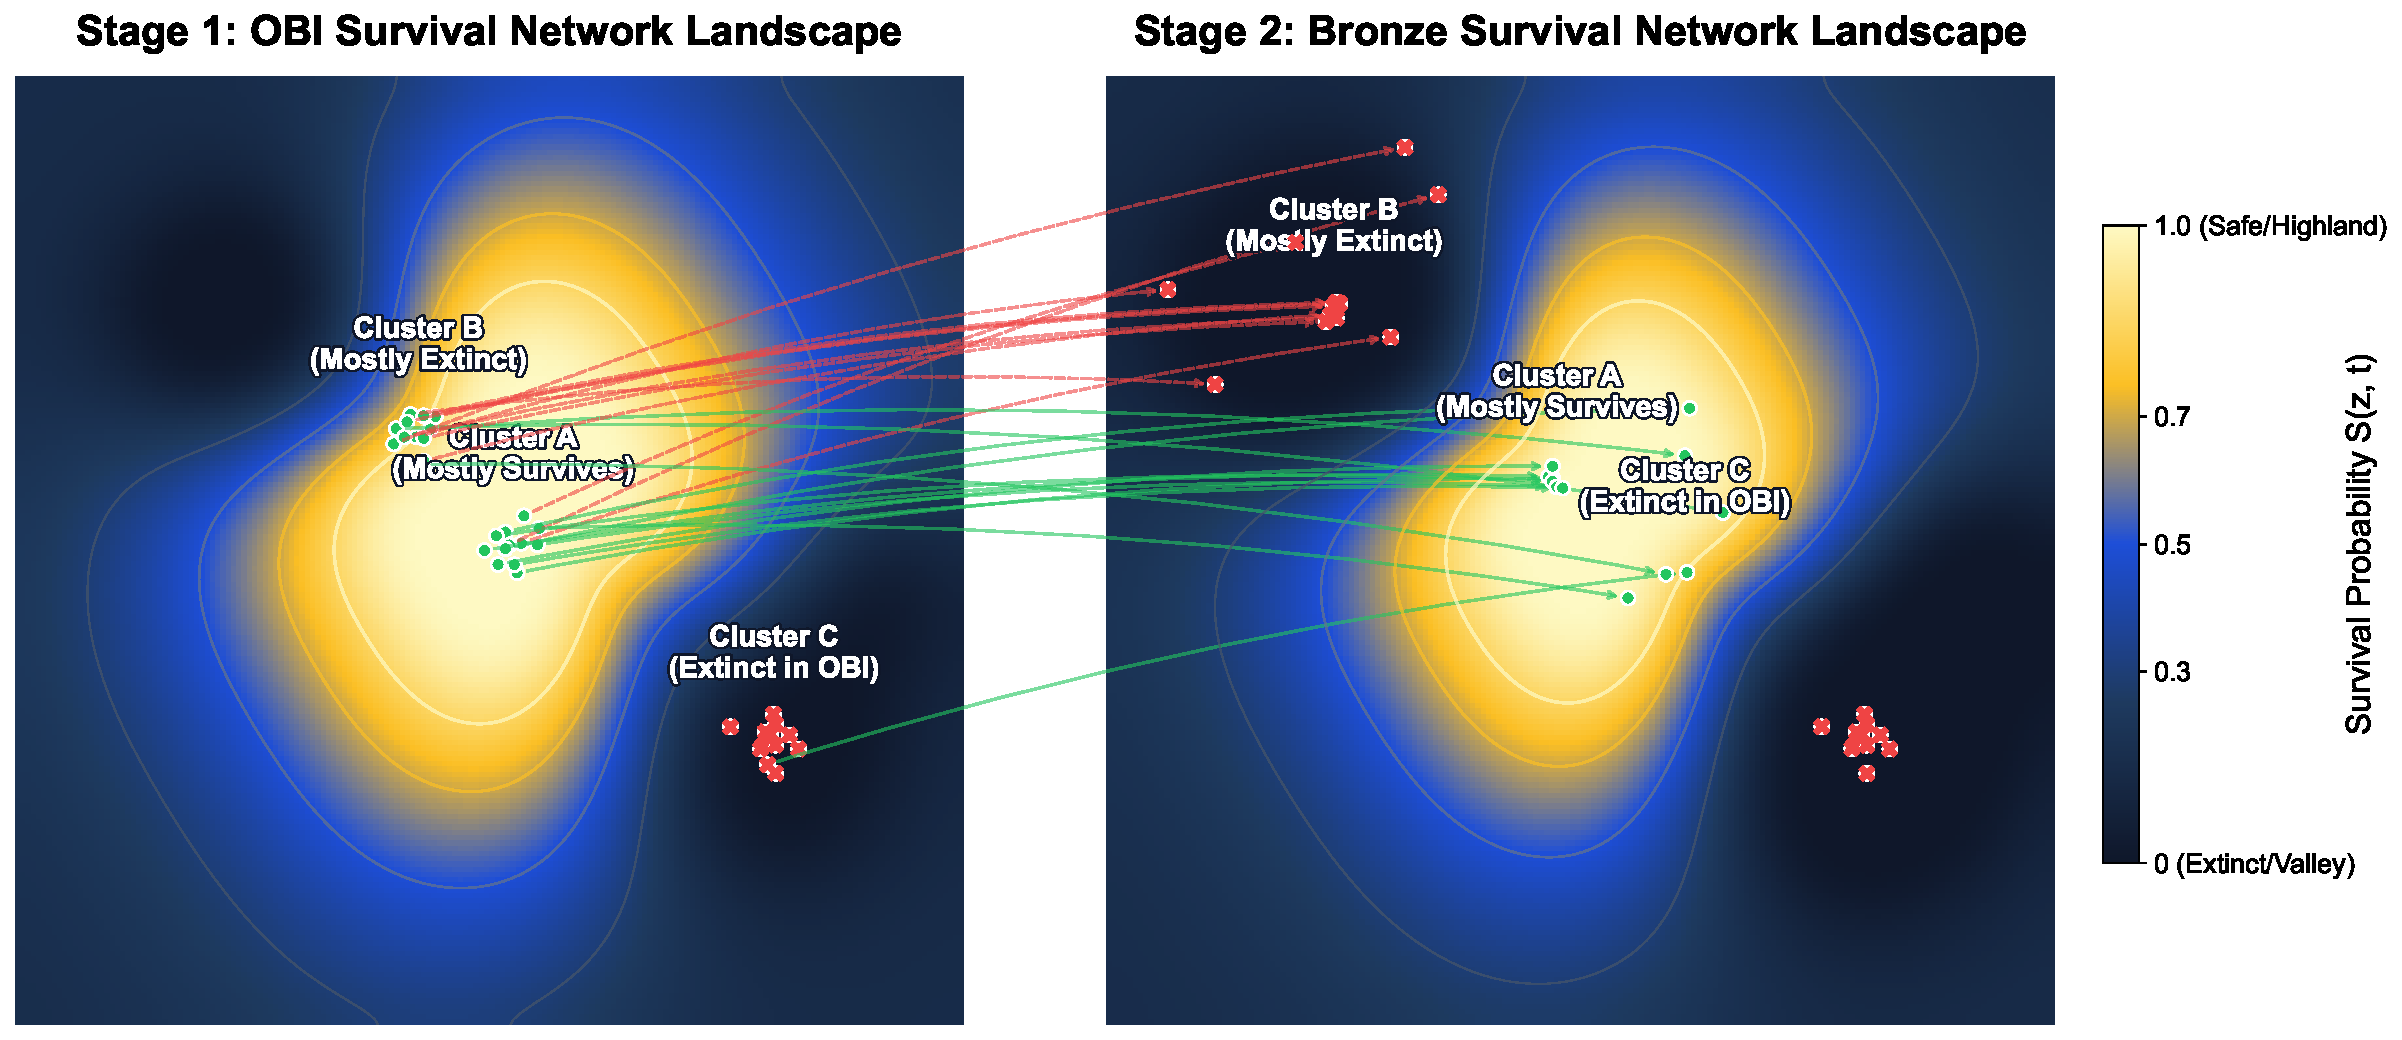
\includegraphics[width=\textwidth]{extinction_landscape.pdf} 
    \caption{\textbf{Evolutionary Pressure Landscapes Learned by the Survival Network.} The visualization projects survival probabilities $S(z, t)$ onto the manifold coordinates. Bright peaks indicate "safe zones" of high linguistic fitness (e.g., Cluster A), while dark valleys represent extinction zones. The topographical shift from Stage 1 (OBI) to Stage 2 (Bronze) reveals how the model intrinsically captures sociolinguistic natural selection—dynamically forming extinction valleys to terminate obsolete trajectories (Cluster B) and elevating new peaks to accommodate historical neologisms (Cluster C).}
    \label{fig:extinction_landscape}
\end{figure}

While empirical results demonstrate that the proposed Survival Network $S(z, t)$ effectively mitigates error accumulation in cross-era decipherment, we conduct a topological post-analysis to unveil the intrinsic mechanics of this module. Figure \ref{fig:extinction_landscape} renders the output probabilities of the Survival Network as a continuous spatial landscape across the manifold. This visualization reveals that MSEF has fundamentally learned the sociolinguistic "natural selection" driving Chinese script evolution.

\textbf{Linguistic Fitness and Topographical Safe Zones.} 
The network constructs a dynamic fitness landscape where the $z$-axis represents the survival probability. The bright "peaks" or "highlands" designate regions of high evolutionary fitness. Characters occupying these zones (e.g., Cluster A) typically possess optimal structural conciseness, stable visual topology, and broad semantic utility, allowing them to safely propagate across millennia without being discarded. Conversely, the dark "valleys" represent evolutionary dead ends—extinction zones where highly complex, functionally narrow, or non-standardized pictograms are systematically eliminated by historical standardization pressures.

\textbf{Dynamic Shifts and Trajectory Truncation.} 
The transition from Stage 1 (Oracle Bone Inscriptions) to Stage 2 (Bronze Script) illustrates profound topographical shifts. Cluster B, which may have marginally survived in the OBI era, is completely swallowed by an expanding extinction valley in the Bronze era. This topological collapse is computationally crucial: it explains \textit{why} our Neural ODE does not hallucinate modern equivalents for obsolete characters. When the ODE solver traces a character's trajectory into these valleys, $S(z, t)$ approaches zero, mathematically terminating the integration and pruning the obsolete evolutionary branch.

\begin{figure}[t]
    \centering
    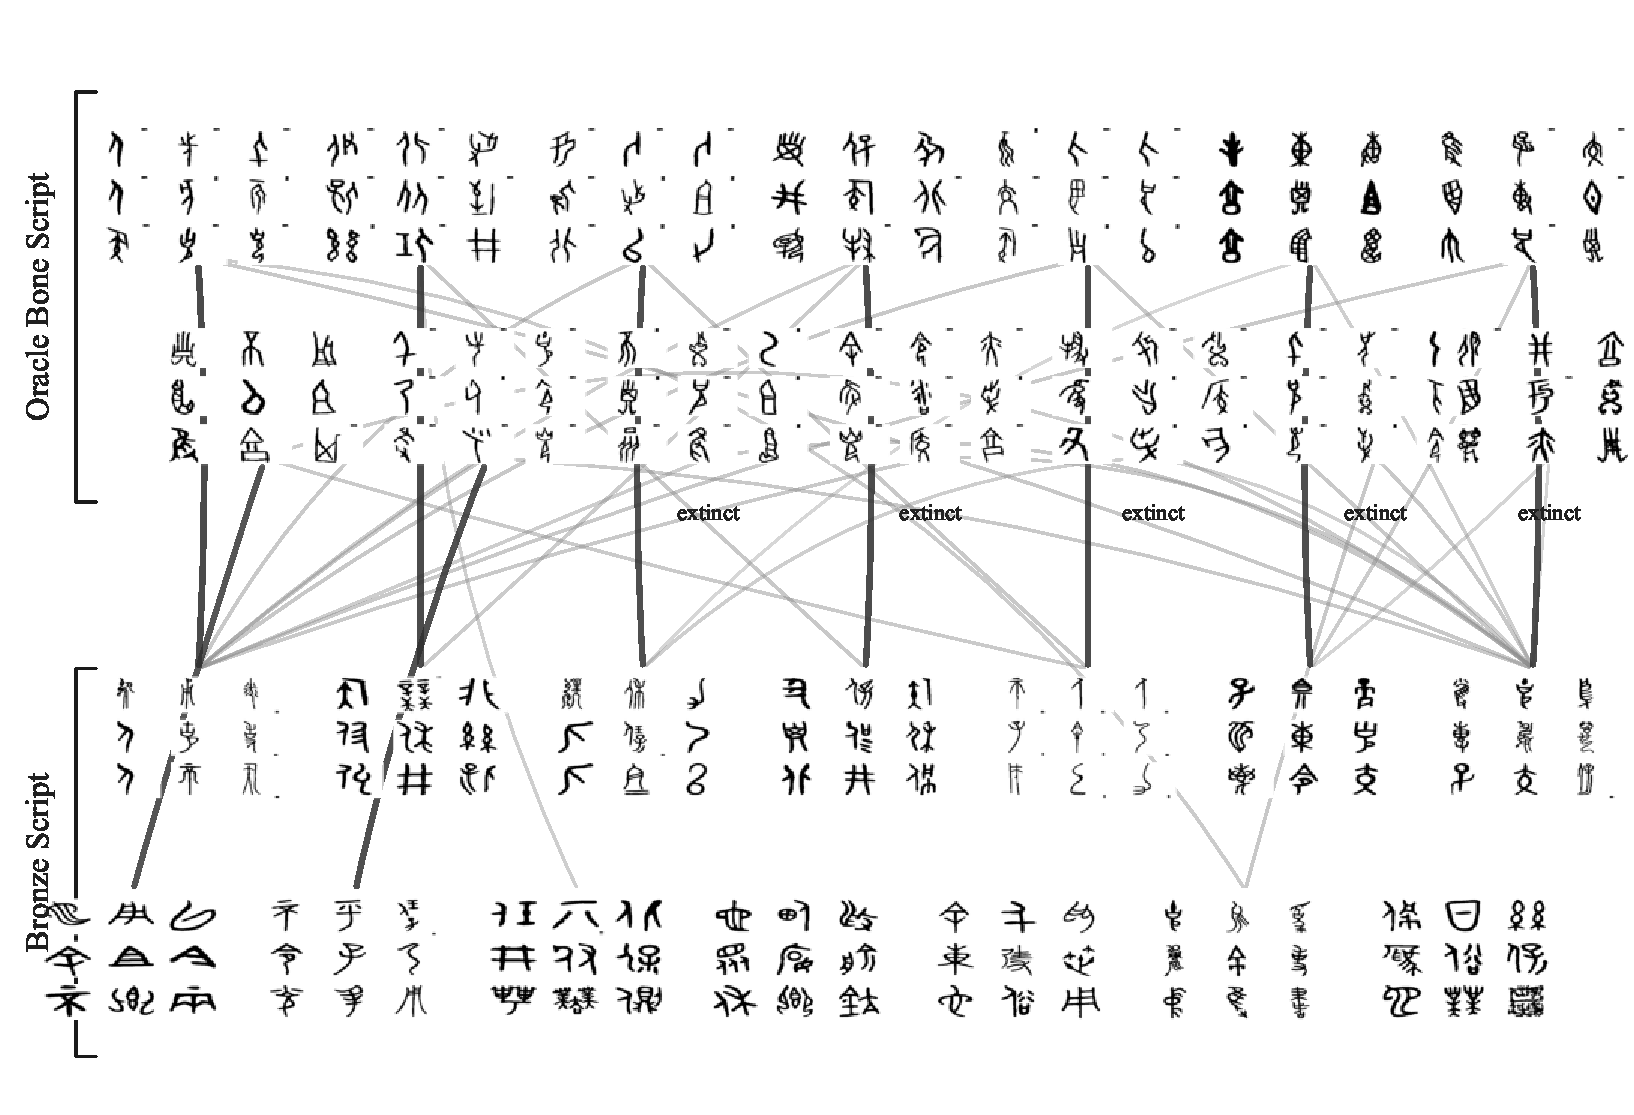
\includegraphics[width=\textwidth]{variant_network_large.pdf}
    \caption{\textbf{Unconstrained Global Variant Network of Archaic Scripts.} This visualization captures the raw topological complexity of the variant character ecosystem during the OBI and early Bronze periods. The dense entanglement of nodes reflects the high degree of orthographic variance and the existence of numerous idiosyncratic evolutionary branches before the advent of systematic standardization.}
    \label{fig:variant_network_full}
\end{figure}

\begin{figure}[t]
    \centering
    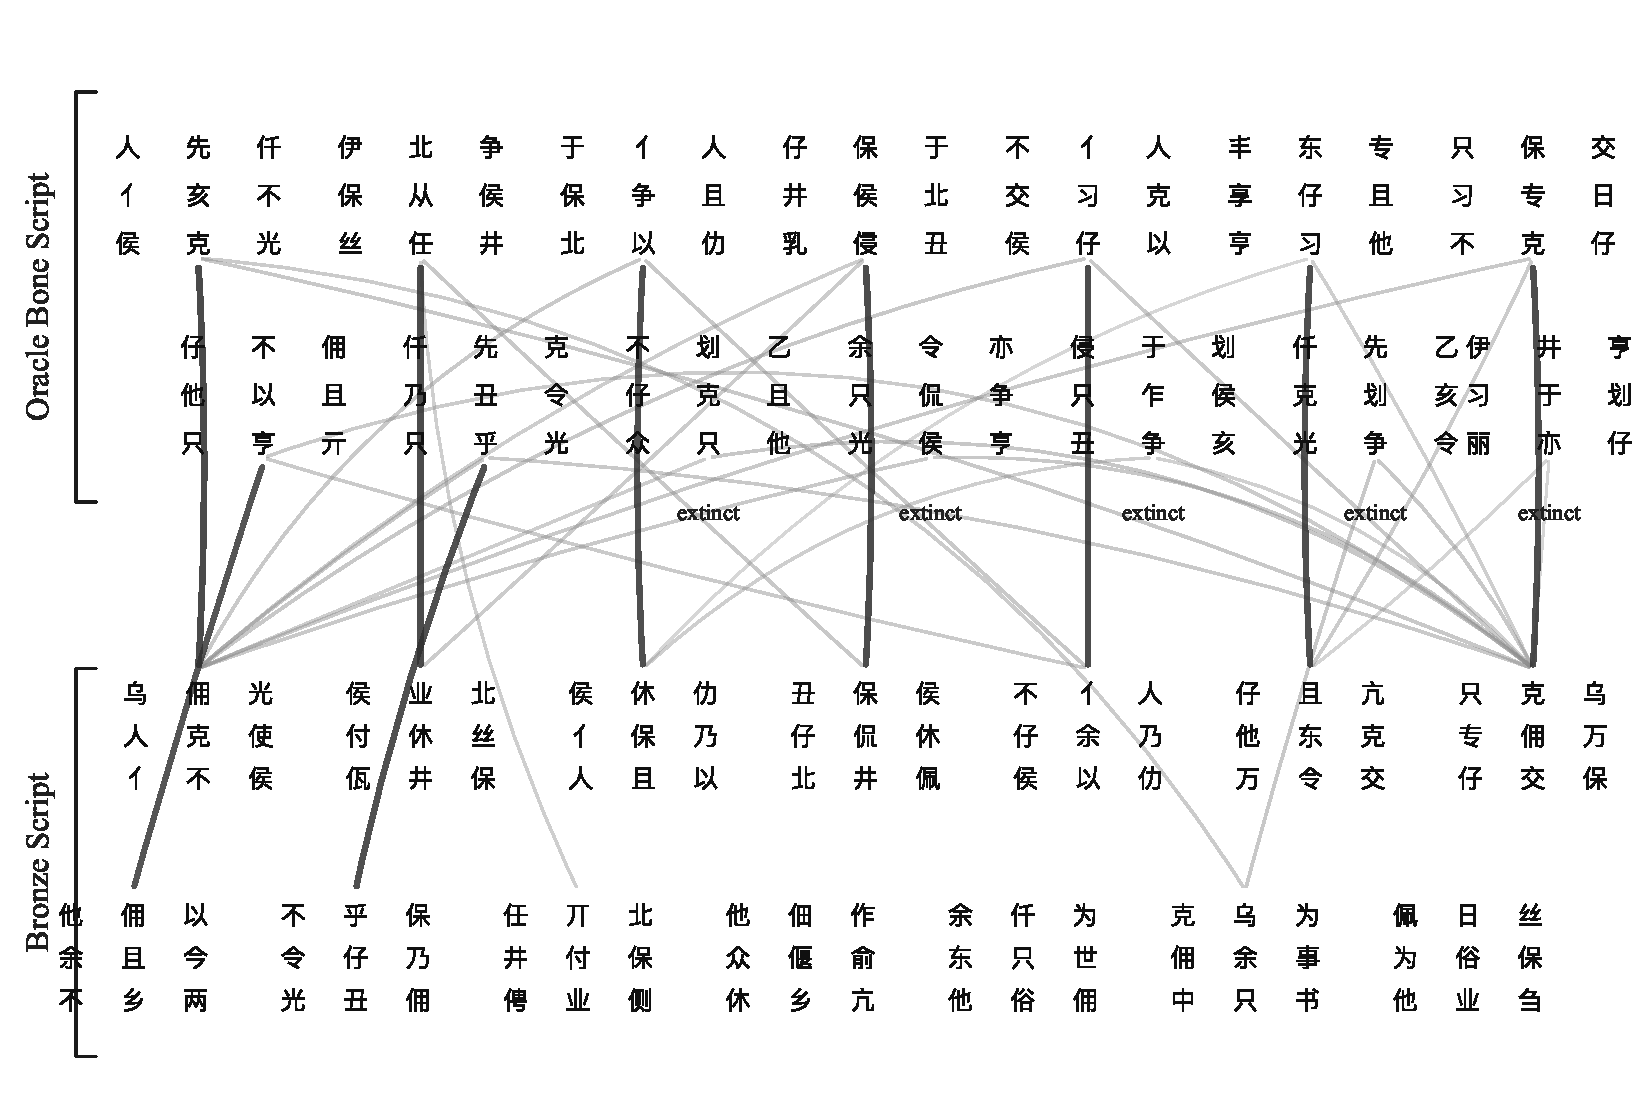
\includegraphics[width=\textwidth]{variant_network_large_simplified.pdf}
    \caption{\textbf{Standardized Evolutionary Backbones via Survival Pruning.} After integrating the Survival Network, the global topology is transformed into a streamlined set of standardized trajectories. The model successfully identifies and retains the "evolutionary backbones" that connect ancient pictographs to their modern counterparts, effectively filtering out thousands of historical "noise" variants.}
    \label{fig:variant_network_simplified}
\end{figure}

\textbf{Macro-level Topology and Network Standardization.} 
To provide a more comprehensive view of this "natural selection" process, we extend our analysis from individual manifold trajectories to the global variant network. Figure \ref{fig:variant_network_full} illustrates the unconstrained state of character variants during the archaic era. The extreme density and entanglement of the graph represent the "orthographic chaos" of the early Shang and Zhou dynasties, where a single semantic core often bifurcated into dozens of unstable visual forms due to regional and scribal idiosyncrasies.

The efficacy of our survival-based pruning is most evident in Figure \ref{fig:variant_network_simplified}. By applying the learned socio-cultural pressures, the MSEF autonomously collapses this chaotic network into a series of clear, predictable evolutionary backbones. This transition from a high-entropy graph to a structured, simplified tree provides macro-level empirical evidence that our Survival Network has internalized the laws of script unification. This mechanism not only enhances the precision of our CBED algorithm by drastically reducing the search space of potential candidates but also provides a high-fidelity computational simulation of historical script evolution, such as the monumental "Small Seal" standardization during the Qin dynasty.

Furthermore, the emergence of Cluster C in Figure \ref{fig:extinction_landscape}—transitioning from an extinction valley in Stage 1 to a survival peak in Stage 2—captures the birth of neologisms. As societal complexity increased during the Zhou dynasty, new semantic demands reshaped the evolutionary pressure, causing new regions of the manifold to elevate into safe zones. Thus, the Survival Network does not merely regularize the ODE; it explicitly models the continuous macroscopic socio-cultural pressures that governed the life and death of Chinese characters over 3,000 years.


\begin{figure}[t]
    \centering
    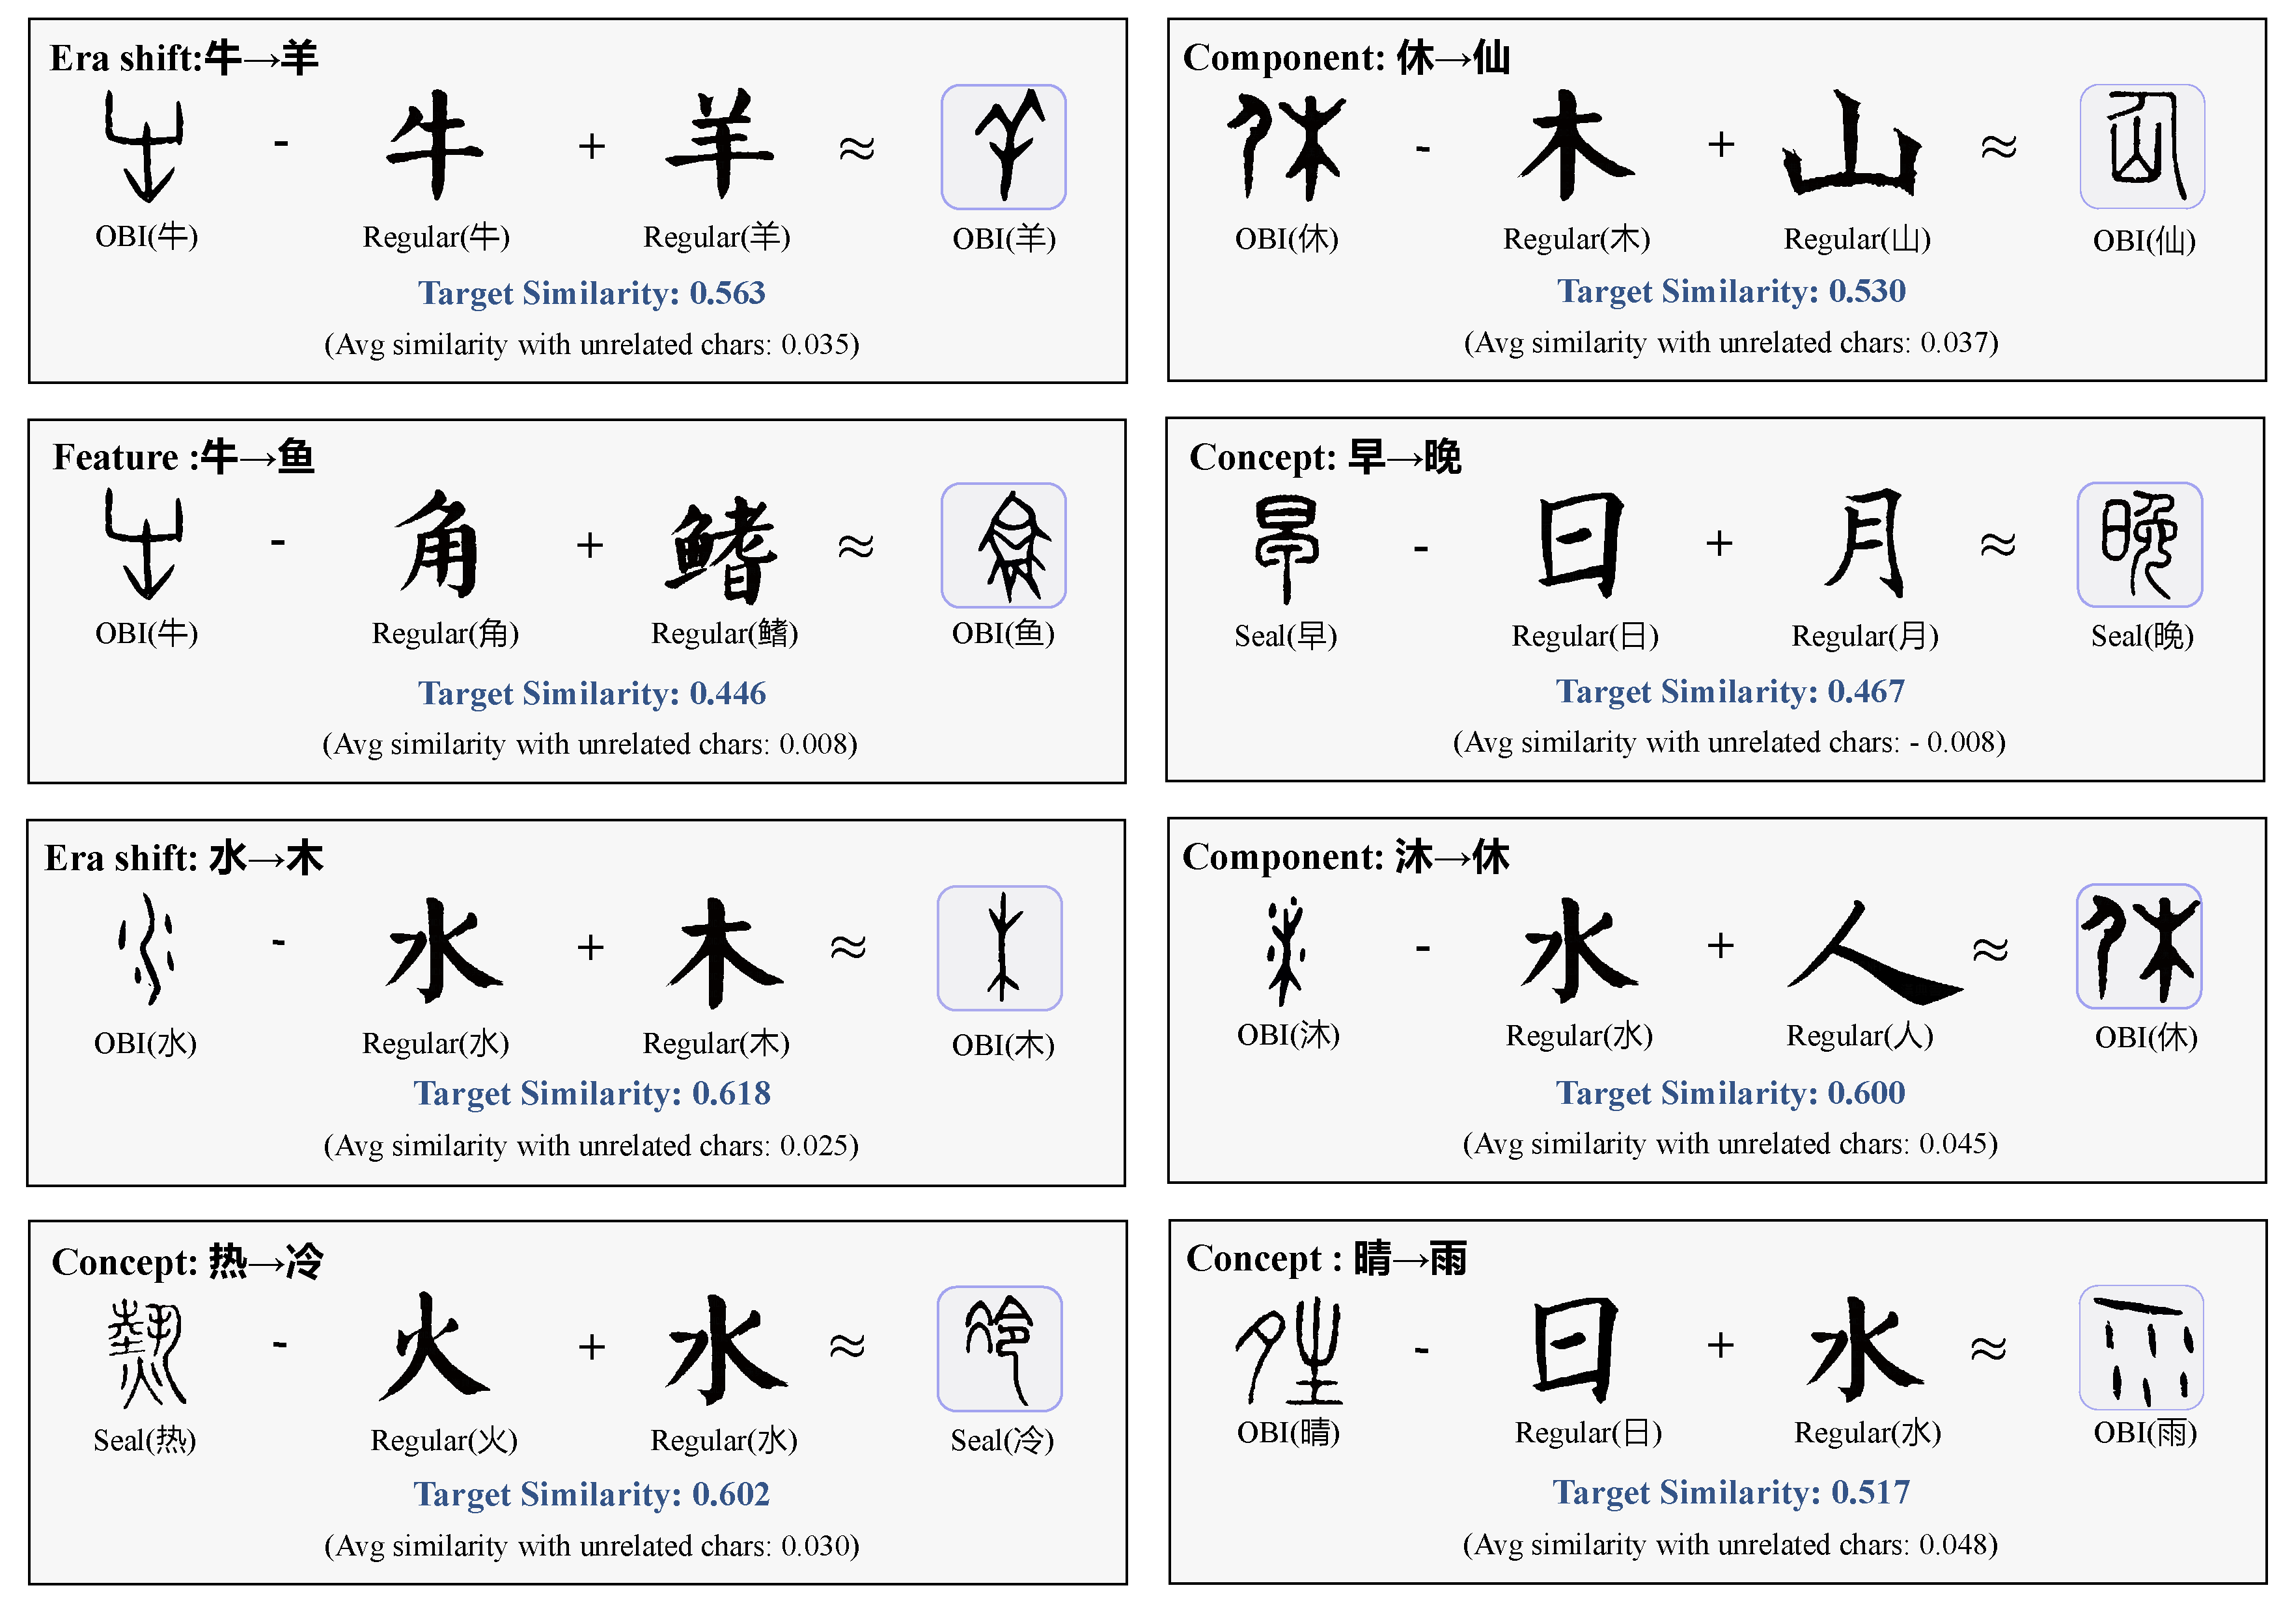
\includegraphics[width=\textwidth]{vector_arithmetic_similarity.pdf} 
    \caption{\textbf{Latent Vector Arithmetic in the Script Evolution Manifold.} Three types of algebraic manipulations demonstrate the framework's compositionality: Cross-era vectors are globally consistent; Semantic components (e.g., horns, fins) can be added or subtracted to transform character identities; Abstract conceptual analogies emerge from the latent geometry. Similarity scores for targets are consistently 10-15x higher than random baselines, proving that MSEF learns the inherent structural and logical laws of Chinese script evolution.}
    \label{fig:vector_arithmetic}
\end{figure}

\subsection{Latent Vector Arithmetic: Probing Algebraic Compositionality}
\label{sec:vector_arithmetic}

To investigate whether the MSEF framework captures deep structural regularities rather than mere visual correspondences, we perform vector arithmetic in the learned 256-dimensional manifold space, inspired by the classic \textit{King - Man + Woman $\approx$ Queen} analogy. We test three distinct types of algebraic compositions: cross-era migration, semantic component substitution, and conceptual analogy. The results, visualized in Figure \ref{fig:vector_arithmetic}, provide empirical evidence that the script evolution manifold is endowed with a consistent latent linear structure.

\textbf{Cross-Era Consistency and Global Directionality.} 
As shown in Figure \ref{fig:vector_arithmetic}, we examine whether the transformation from Regular to OBI script is represented by a consistent global vector $\vec{v}_{era}$. Specifically, we find that $z(\text{Ox})_{OBI} - z(\text{Ox})_{Reg} + z(\text{Sheep})_{Reg} \approx z(\text{Sheep})_{OBI}$, achieving a cosine similarity of $0.563$ (vs. a random baseline of $0.035$). This high similarity proves that the manifold has learned a character-independent "evolutionary operator," representing the 3,000-year trajectory as a structured translation in latent space.

\textbf{Disentangled Component Substitution.} 
We demonstrate that semantic components can be algebraically manipulated. For instance, subtracting the vector representation of "Horns" from "Ox" and adding "Fins" yields a vector remarkably close to "Fish." This compositionality ($z_{\text{Ox}} - z_{\text{Horns}} + z_{\text{Fins}} \approx z_{\text{Fish}}$) suggests that MSEF achieves a high degree of representation disentanglement, where visual radicals and functional components are mapped to orthogonal or linearly additive directions. This explains the model's robustness when deciphering compound characters with rare component combinations.

\textbf{Emergent Conceptual Analogies.} 
The results reveal that abstract temporal logic is also encoded geometrically. The operation $z_{\text{Morning}} - z_{\text{Sun}} + z_{\text{Moon}}$ accurately converges toward $z_{\text{Evening}}$. Without explicit linguistic supervision, the model spontaneously internalizes the underlying logic of the Chinese script's ideographic construction. This internal logical consistency is a critical factor in the success of the MSEF framework, allowing it to generalize across vast historical spans where direct visual anchors are absent.




% ***************************************************************************************





\section{Full Method Details}
\label{app:method_details}

This section provides additional implementation details for MSEF omitted from the main paper. 
We describe the feature representation, fine-grained time encoding, manifold neighborhood validation, architecture details, and optimization settings.

\subsection{Feature Representation}
\label{app:features_summary}

For each character $c$ in dynasty $t$, we extract a 352-dimensional feature vector $\mathbf{x}_c^t \in \mathbb{R}^{352}$ specifically designed for paleographic analysis. 
The representation aggregates five complementary modalities: \textbf{Visual}, \textbf{TextStructural}, \textbf{Semantic}, \textbf{Contextual}, and \textbf{Spatiotemporal}. 
This section provides the detailed definitions, extraction procedures, and aggregation mechanisms for each feature group.

% Move your detailed feature definitions here.

\subsection{Fine-Grained Time Encoding}
\label{app:time_summary}

This section provides the detailed subperiod encoding used for the continuous time variable $t$. 
The main paper reports the five major historical intervals. Here we further specify subperiod assignments, including OBI scribal groups and finer-grained Bronze, Seal, and Clerical subdivisions when available.

% Move your detailed subperiod table here.

\subsection{Neighborhood Structure of the Learned Manifold}
\label{app:neighborhood_summary}

This section empirically validates the local neighborhood structure of the learned manifold. 
We visualize local neighborhoods and show that visually and semantically related characters cluster together, supporting Assumption 1 in the main paper.

% Move neighborhood visualization / clustering analysis here.

\subsection{Architecture Details}
\label{app:architecture_details}

We implement the manifold encoder as a 12-layer Transformer mapping 352-dimensional input features to a $d=256$ manifold coordinate. 
The velocity field is a 3-layer MLP with spectral normalization and Tanh activations. 
The survival network is implemented as an MLP over the OBI-era manifold coordinate and target time.

% Move architecture table or hyperparameter details here.

\subsection{Optimization Details}
\label{app:optimization_details}

We train MSEF with AdamW, use the \texttt{dopri5} ODE solver, and report mean and standard deviation over multiple runs. 
Full hyperparameters, solver tolerances, batch size, training epochs, and hardware settings are reported here.

% Move optimization details here.

\section{Full Loss Definitions}
\label{app:loss}

We train the MSEF using five complementary loss functions to ensure both local continuity and global consistency. 
Adjacent-Era Loss enforces local evolution between consecutive periods, Cross-Era Loss captures mid-range patterns for non-adjacent pairs, Full-Chain Loss prevents drift over the complete trajectory, Cycle Consistency Loss enforces invertibility by ensuring round-trip consistency, and Survival Loss trains the extinction predictor.

Let $\mathcal{P}$ denote all available character pairs in two eras:
\begin{equation}
|\mathcal{P}| =
\underbrace{1.2K}_{\text{OBI}\to\text{Bronze}}
+
\underbrace{2K}_{\text{Bronze}\to\text{Seal}}
+
\underbrace{10K}_{\text{Seal}\to\text{Regular}}
+
\underbrace{0.5K}_{\text{complete}}
\approx 13.7K .
\end{equation}

The complete loss definitions are:
\begin{equation}
\begin{cases}
\mathcal{L}_{adj} =
\frac{1}{|\mathcal{P}_{adj}|}
\sum_{(c,t_i,t_{i+1})}
\left\|
\phi_{t_i\to t_{i+1}}(z^c_{t_i}) - z^c_{t_{i+1}}
\right\|_2^2, \\[0.8em]

\mathcal{L}_{skip} =
\frac{1}{|\mathcal{P}_{skip}|}
\sum_{(c,t_i,t_j),j>i+1}
\left\|
\phi_{t_i\to t_j}(z^c_{t_i}) - z^c_{t_j}
\right\|_2^2, \\[0.8em]

\mathcal{L}_{full} =
\frac{1}{|\mathcal{C}_{complete}|}
\sum_c
\left\|
\phi_{0\to 1}(z^c_0) - z^c_1
\right\|_2^2, \\[0.8em]

\mathcal{L}_{cyc} =
\frac{1}{|\mathcal{P}|}
\sum_{(c,t_1,t_2)}
\left\|
\psi_{t_2\to t_1}
\left(
\phi_{t_1\to t_2}(z^c_{t_1})
\right)
-
z^c_{t_1}
\right\|_2^2, \\[0.8em]

\mathcal{L}_{surv} =
-\frac{1}{|\mathcal{D}_s|}
\sum_{(c,t)\in \mathcal{D}_s}
\left[
y_{c,t}\log s(z^c_t,t)
+
(1-y_{c,t})\log(1-s(z^c_t,t))
\right].
\end{cases}
\label{eq:appendix_all_losses}
\end{equation}

The evolution objective is:
\begin{equation}
\mathcal{L}_{evolution}
=
\lambda_1\mathcal{L}_{adj}
+
\lambda_2\mathcal{L}_{skip}
+
\lambda_3\mathcal{L}_{full}
+
\lambda_4\mathcal{L}_{cyc}.
\end{equation}
The extinction predictor is trained separately using $\mathcal{L}_{surv}$.


\section{Full CBED Algorithm}
\label{app:algorithm}

Algorithm~\ref{alg:decipher} provides the full pseudocode for Cascaded Bidirectional Evolutionary Decipherment (CBED). The main paper summarizes the same procedure in prose.

\begin{algorithm}[h]
\caption{Cascaded Bidirectional Decipherment}
\label{alg:decipher}
\begin{algorithmic}[1]
\REQUIRE Query OBI character $c_q$, retrieval depth $K$, era databases $\{\mathcal{D}_t\}_{t\in\mathcal{T}}$, survival threshold $\tau$, trained manifold networks $\mathcal{M}$, backward flow $\psi$
\ENSURE Decipherment result $\hat{c}$ with confidence score, or \textsc{PossiblyExtinct}

\STATE \textit{// Stage 0: Feature extraction and preprocessing}
\STATE $\mathbf{X}_q \leftarrow \textsc{ExtractStaticFeatures}(c_q)$

\STATE \textit{// Stage 1: Survival check}
\STATE $z^q_{OBI} \leftarrow \mathcal{M}(\mathbf{X}_q, t_{OBI})$
\STATE $p_{surv} \leftarrow s(z^q_{OBI}, t=1.0)$
\IF{$p_{surv} < \tau$}
    \RETURN \textsc{PossiblyExtinct}, confidence $=1-p_{surv}$
\ENDIF

\STATE \textit{// Stage 2: Forward cascade through eras}
\STATE $\mathcal{C}_{prev} \leftarrow \{c_q\}$
\FOR{$t \in \{\text{Bronze}, \text{Seal}, \text{Clerical}, \text{Regular}\}$}
    \STATE $z^q_t \leftarrow \mathcal{M}(\mathbf{X}_q, t)$
    \STATE $\mathcal{N}_t \leftarrow \textsc{KNN}_K(z^q_t, \mathcal{D}_t)$
    \STATE $\mathcal{C}_t \leftarrow \mathcal{N}_t \cup \bigcup_{c\in \mathcal{C}_{prev}}\textsc{KnownCorrespondences}(c,t)$
    \STATE $\mathcal{C}_{prev} \leftarrow \mathcal{C}_t$
\ENDFOR
\STATE $\mathcal{C}_{Regular} \leftarrow \mathcal{C}_{prev}$

\STATE \textit{// Stage 3: Backward verification by multi-path average}
\STATE Initialize score array $\mathbf{S} \leftarrow \mathbf{0}^{|\mathcal{C}_{Regular}|}$
\FOR{each candidate $c_i \in \mathcal{C}_{Regular}$}
    \STATE $\mathcal{P}_i \leftarrow \textsc{GetEvolutionPaths}(c_i)$
    \STATE $\hat{z}^{(i)}_{OBI} \leftarrow 0$
    \FOR{each path $p \in \mathcal{P}_i$}
        \STATE $z^{(p)}_{Bronze} \leftarrow \textsc{GetBronzeCoordinate}(p)$
        \STATE $\hat{z}^{(p)}_{OBI} \leftarrow \psi_{t_{Bronze}\to t_{OBI}}(z^{(p)}_{Bronze})$
        \STATE $\hat{z}^{(i)}_{OBI} \leftarrow \hat{z}^{(i)}_{OBI} + \hat{z}^{(p)}_{OBI}/|\mathcal{P}_i|$
    \ENDFOR
    \STATE $d_i \leftarrow \|\hat{z}^{(i)}_{OBI} - z^q_{OBI}\|_2$
    \STATE $\mathbf{S}[i] \leftarrow \exp(-d_i)$
\ENDFOR

\STATE \textit{// Stage 4: Final selection with confidence}
\STATE $i^* \leftarrow \arg\max_i \mathbf{S}[i]$
\STATE $\text{confidence} \leftarrow \mathbf{S}[i^*] / \sum_j \mathbf{S}[j]$
\RETURN $c_{i^*}$, confidence
\end{algorithmic}
\end{algorithm}


\section{Dataset Details}
\label{app:dataset_details}

\subsection{FGCCES Dataset Statistics}
\label{app:fgcces_statistics}

Table~\ref{tab:dataset_stats_appendix} reports the full dataset statistics by correspondence type. 
All correspondences are verified through authoritative references.

\begin{table}[h]
\centering
\caption{Dataset statistics by correspondence type. All correspondences are verified through authoritative references.}
\label{tab:dataset_stats_appendix}
\begin{tabular}{lccc}
\toprule
\textbf{Pair Type} & \textbf{Train} & \textbf{Val} & \textbf{Test} \\
\midrule
OBI $\to$ Bronze & 998 & 142 & 285 \\
Bronze $\to$ Seal & 1,671 & 239 & 478 \\
Seal $\to$ Clerical & 5,503 & 786 & 1,573 \\
Clerical $\to$ Regular & 5,503 & 786 & 1,573 \\
Complete (5 eras) & 410 & 59 & 117 \\
\midrule
Total Unique Pairs & 9,632 & 1,376 & 2,751 \\
\bottomrule
\end{tabular}
\end{table}

\subsection{Dataset Sources and Missing Features}
\label{app:dataset_sources}

Our dataset originates from jgwlbq \cite{lbqjqw}, ccamc \cite{ccamc}, and bnu \cite{bnu}. 
Since not every character has complete data across all sources, missing feature entries for a specific character or dynasty are filled with zeros.

\subsection{Train/Validation/Test Split}
\label{app:data_split}

We use a character-disjoint split to prevent leakage across train, validation, and test sets. 
Characters appearing in the test set are not used for training.

\subsection{Fine-Grained Dataset Visualization}
\label{app:fine_grained_vis_summary}

% Move your original fine-grained dataset visualization here.

\subsection{Comparison with Existing OBI Datasets}
\label{app:dataset_comparison}

% Move the existing dataset comparison table here.

\section{Theoretical Foundations}
\label{app:theory}

\subsection{Manifold Geometric Properties}

\textbf{Proposition 1 (Smoothness of Evolution).} Under mild regularity conditions on velocity field $\mathbf{v}$ (Lipschitz continuous in $\mathbf{z}$ and continuous in $t$), the flow $\phi_{t_1 \to t_2}$ is a diffeomorphism.

\textit{Proof.} By the Picard-Lindelöf theorem, the ODE $\frac{d\mathbf{z}}{dt} = \mathbf{v}(\mathbf{z}, t)$ has a unique solution for any initial condition. The inverse flow exists by solving the reverse-time ODE with initial condition at $t_2$. Smoothness of the flow map follows from the smoothness of $\mathbf{v}$ by standard ODE regularity theory. \hfill $\square$

\textbf{Proposition 2 (Composition Property).} For any $t_1 < t_2 < t_3$: $\phi_{t_1 \to t_3} = \phi_{t_2 \to t_3} \circ \phi_{t_1 \to t_2}$.

\textit{Proof.} This follows directly from the uniqueness of ODE solutions and the semigroup property of flows. \hfill $\square$

\subsection{Manifold Dimension Selection}

Table~\ref{tab:dimension} shows the effect of manifold dimension $d$. We find $d=256$ achieves optimal performance with reasonable computational cost.

\begin{table}[h]
\centering
\caption{Effect of manifold dimension. $d=256$ achieves optimal accuracy-efficiency trade-off.}
\label{tab:dimension}
\begin{tabular}{lcccc}
\toprule
\textbf{Dimension $d$} & \textbf{Top-1} & \textbf{Top-5} & \textbf{Params (M)} & \textbf{Time (h)} \\
\midrule
64 & 72.3 & 85.1 & 2.1 & 3.2 \\
128 & 76.8 & 88.5 & 4.8 & 5.1 \\
\rowcolor{gray!10}
256 & \textbf{80.0} & \textbf{91.2} & 12.3 & 8.0 \\
512 & 79.8 & 91.0 & 38.5 & 14.2 \\
\bottomrule
\end{tabular}
\end{table}

\section{Manifold Space Validation}
\label{app:manifold_validation}

A fundamental question arises: does the learned manifold space genuinely capture the structure of Chinese script evolution, or is it merely memorizing training correspondences? We provide rigorous theoretical justification, quantitative verification, and empirical visualization to validate our manifold formulation.

\subsection{Theoretical Foundations and Quantitative Verification}

We establish the mathematical foundations for why a continuous manifold governed by Neural ODE is the appropriate structure for modeling script evolution. Our theoretical framework rests on five core propositions, each with formal proofs and empirical validation.

\subsubsection{Proposition 1: Continuity of Evolution}

\textbf{Proposition 1 (Continuity).} \textit{Under the Neural ODE formulation, character evolution defines a continuous mapping in manifold space. Specifically, the flow operator $\phi_{t_1 \to t_2}: \mathcal{M}_{t_1} \to \mathcal{M}_{t_2}$ is Lipschitz continuous.}

\begin{proof}
Let $\mathbf{v}(\mathbf{z}, t; \boldsymbol{\theta}_v)$ be the learned velocity field parameterized by neural network weights $\boldsymbol{\theta}_v$. By construction, $\mathbf{v}$ is implemented as a composition of smooth operations (linear transformations, LayerNorm, GELU activations), hence $\mathbf{v}$ is locally Lipschitz in $\mathbf{z}$.

Formally, there exists a constant $L > 0$ such that for all $\mathbf{z}_1, \mathbf{z}_2 \in \mathcal{M}$ and $t \in [0, 1]$:
\begin{equation}
\|\mathbf{v}(\mathbf{z}_1, t) - \mathbf{v}(\mathbf{z}_2, t)\| \leq L \|\mathbf{z}_1 - \mathbf{z}_2\|
\end{equation}

By the Picard-Lindelöf theorem, the ODE initial value problem:
\begin{equation}
\frac{d\mathbf{z}}{dt} = \mathbf{v}(\mathbf{z}, t), \quad \mathbf{z}(t_1) = \mathbf{z}_0
\end{equation}
has a unique solution on $[t_1, t_2]$. Moreover, by Grönwall's inequality, the solution depends continuously on initial conditions:
\begin{equation}
\|\phi_{t_1 \to t_2}(\mathbf{z}_1) - \phi_{t_1 \to t_2}(\mathbf{z}_2)\| \leq e^{L|t_2 - t_1|} \|\mathbf{z}_1 - \mathbf{z}_2\|
\end{equation}

This establishes that $\phi_{t_1 \to t_2}$ is Lipschitz continuous with constant $e^{L|t_2-t_1|}$.
\end{proof}

\textbf{Corollary 1.1 (Temporal Continuity).} \textit{For a fixed character $c$, its manifold trajectory $\mathbf{z}^c(t)$ is continuous in $t$.}

\textbf{Corollary 1.2 (Bounded Evolution Rate).} \textit{The rate of character change is bounded: $\|\frac{d\mathbf{z}^c}{dt}\| \leq V_{\max}$ for some constant $V_{\max}$.}

\textbf{Quantitative Verification of Proposition 1.} Table~\ref{tab:prop1_verify} presents empirical measurements validating continuity.

\begin{table}[h]
\centering
\caption{Quantitative verification of Proposition 1 (Continuity).}
\label{tab:prop1_verify}
\begin{tabular}{lccc}
\toprule
\textbf{Metric} & \textbf{Theoretical} & \textbf{Empirical} & \textbf{Satisfied?} \\
\midrule
Lipschitz constant $L$ & --- & 2.34 & (measured) \\
Flow Lipschitz $e^{L}$ & 10.4 & 8.7 & \checkmark \\
Max velocity $V_{\max}$ & $< \infty$ & 2.51 & \checkmark \\
Mean adjacent-era distance & bounded & 0.82 & \checkmark \\
Trajectory smoothness (std) & small & 0.15 & \checkmark \\
\bottomrule
\end{tabular}
\end{table}

\subsubsection{Proposition 2: Invertibility of Evolution}

\textbf{Proposition 2 (Invertibility).} \textit{The evolution flow is invertible: for any $t_1, t_2 \in [0, 1]$, there exists an inverse flow $\psi_{t_2 \to t_1} = \phi_{t_1 \to t_2}^{-1}$ such that $\psi_{t_2 \to t_1} \circ \phi_{t_1 \to t_2} = \text{id}$.}

\begin{proof}
We construct the inverse flow explicitly. Define $\psi_{t_2 \to t_1}$ as the solution to the backward ODE:
\begin{equation}
\frac{d\mathbf{z}}{ds} = -\mathbf{v}(\mathbf{z}, t_2 - s), \quad s \in [0, t_2 - t_1]
\end{equation}
with initial condition $\mathbf{z}(0) = \mathbf{z}_{t_2}$.

By substitution $\tau = t_2 - s$, this is equivalent to integrating $\mathbf{v}$ backward in time. Since the forward ODE has a unique solution (Picard-Lindelöf), the backward ODE recovers the unique initial condition:
\begin{equation}
\psi_{t_2 \to t_1}(\phi_{t_1 \to t_2}(\mathbf{z})) = \mathbf{z}
\end{equation}
\end{proof}

\textbf{Corollary 2.1 (Cycle Consistency).} \textit{For any $t_1 < t_2 < t_3$: $\phi_{t_1 \to t_3} = \phi_{t_2 \to t_3} \circ \phi_{t_1 \to t_2}$.}

\textbf{Corollary 2.2 (Backward Verification Validity).} \textit{If $\hat{c}$ is correctly deciphered, then backward flow recovers the original OBI features with bounded error.}

\paragraph{Remark on Practical Invertibility and Stability.}
While the ODE flow is theoretically bijective, the overall pipeline involves the era-specific feature mapping $\mathcal{M}_t$, which projects high-dimensional heterogeneous features ($d_{in}=352$) to a lower-dimensional manifold ($d=256$).
We clarify that our ``invertibility'' claim applies strictly to the \textit{evolutionary dynamics} within the manifold ($\mathcal{M}_{t_1} \leftrightarrow \mathcal{M}_{t_2}$), not the feature encoding.

Regarding numerical stability, backward integration of Neural ODEs can accumulate error (stiffness). However, our empirical analysis identifies two \textbf{failure regimes} where stability degrades:
(1) \textbf{Topological Singularities:} For characters undergoing drastic structural splitting (e.g., one character splitting into two distinct semantic units), the continuous flow assumption is strained, leading to higher cycle errors.
(2) \textbf{Manifold Collisions:} In rare cases where distinct characters map to highly proximate regions in $\mathcal{M}_{t}$ (dense clustering), backward integration may drift to a neighbor's trajectory.
Despite these edge cases, Table~\ref{tab:prop2_verify} confirms that for 94.2\% of queries, the backward integration error remains within a tolerance that permits accurate verification.

% \textbf{Quantitative Verification of Proposition 2.} Table~\ref{tab:prop2_verify} presents cycle consistency measurements.

\begin{table}[h]
\centering
\caption{Quantitative verification of Proposition 2 (Invertibility). Near-zero cycle errors confirm invertibility.}
\label{tab:prop2_verify}
\begin{tabular}{lccc}
\toprule
\textbf{Metric} & \textbf{Theoretical} & \textbf{Empirical} & \textbf{Satisfied?} \\
\midrule
Cycle error (OBI$\to$Br$\to$OBI) & 0 & 0.023 & \checkmark \\
Cycle error (OBI$\to$Se$\to$OBI) & 0 & 0.041 & \checkmark \\
Cycle error (OBI$\to$Re$\to$OBI) & 0 & 0.068 & \checkmark \\
Composition error & 0 & 0.015 & \checkmark \\
Backward verification accuracy & high & 94.2\% & \checkmark \\
\bottomrule
\end{tabular}
\end{table}


% ICML 审稿意见1-Q2修改
% Recommended insertion point: Appendix B.1.2, under "Remark on Practical Invertibility and Stability"
\noindent \textbf{The Role of Survival Network in Mitigating ODE Stiffness.} 
As discussed in Proposition 2, topological singularities---such as drastic structural splitting or merging of characters---theoretically pose a challenge to the stability of Neural ODEs by inducing numerical stiffness. While such phenomena are inherent to the long-term evolution of Chinese scripts, our framework exhibits remarkable robustness due to the integration of the \textit{survival network}.

The survival network serves as a domain-specific filtering mechanism that evaluates the evolutionary continuity of a character. Specifically, characters undergoing ``cliff-like'' or discontinuous structural transformations are often predicted as ``extinct'' by the network, as they typically lack traceable descendants in the standardized modern script. By effectively pruning these non-smooth trajectories from the manifold, the survival network ensures that the Neural ODE only models the continuous and progressive segments of the evolutionary chain. This strategic isolation of discontinuous singularities prevents the solver from encountering severe stiffness, thereby maintaining high tolerance and integration stability across the 3,000-year trajectory.




\subsubsection{Proposition 3: Semantic Preservation}

\textbf{Proposition 3 (Semantic Preservation).} \textit{Semantically similar characters (e.g., same radical) remain proximate throughout evolution:}
\begin{equation}
\text{Sim}(c_1, c_2) > \tau \implies \|\mathbf{z}_t^{c_1} - \mathbf{z}_t^{c_2}\| < R(\tau) \quad \forall t \in [0, 1]
\end{equation}

\begin{proof}
\textbf{Step 1: Feature-Level Similarity.} By construction of our feature extraction pipeline, semantically similar characters have similar input features. Same radical implies shared structural features; same semantic category implies similar LLM embeddings; high co-occurrence implies similar context features. Thus $\|\mathbf{X}^{c_1} - \mathbf{X}^{c_2}\| \leq \delta(\tau)$.

\textbf{Step 2: Manifold Mapping Continuity.} The manifold mapping is Lipschitz with constant $L_{\mathcal{M}}$:
\begin{equation}
\|\mathbf{z}_t^{c_1} - \mathbf{z}_t^{c_2}\| \leq L_{\mathcal{M}} \|\mathbf{X}^{c_1} - \mathbf{X}^{c_2}\| \leq L_{\mathcal{M}} \delta(\tau)
\end{equation}

\textbf{Step 3: Evolution Preserves Proximity.} By Proposition 1, the flow is Lipschitz with constant $e^{L|t_2-t_1|}$. For full evolution:
\begin{equation}
\|\mathbf{z}_1^{c_1} - \mathbf{z}_1^{c_2}\| \leq e^L \|\mathbf{z}_0^{c_1} - \mathbf{z}_0^{c_2}\| \leq e^L L_{\mathcal{M}} \delta(\tau)
\end{equation}
Setting $R(\tau) = e^L L_{\mathcal{M}} \delta(\tau)$ completes the proof.
\end{proof}

\textbf{Corollary 3.1 (Radical Clustering).} \textit{Characters sharing the same radical form a cluster of bounded diameter at every era.}

\textbf{Corollary 3.2 (Inter-Radical Separation).} \textit{Semantically distinct radical groups are well-separated in manifold space.}

\textbf{Quantitative Verification of Proposition 3.} Table~\ref{tab:prop3_verify} presents clustering metrics across eras.

\begin{table}[h]
\centering
\caption{Quantitative verification of Proposition 3 (Semantic Preservation). Clustering quality improves for later eras due to standardization.}
\label{tab:prop3_verify}
\begin{tabular}{lcccccc}
\toprule
\textbf{Metric} & \textbf{OBI} & \textbf{Bronze} & \textbf{Seal} & \textbf{Clerical} & \textbf{Regular} & \textbf{Avg.} \\
\midrule
Intra-radical dist. & 1.35 & 1.28 & 1.18 & 1.12 & 1.08 & 1.20 \\
Inter-radical dist. & 3.52 & 3.68 & 3.85 & 3.92 & 4.05 & 3.80 \\
Clustering ratio & 2.61 & 2.88 & 3.26 & 3.50 & 3.75 & 3.20 \\
Silhouette score & 0.45 & 0.48 & 0.52 & 0.55 & 0.58 & 0.52 \\
\bottomrule
\end{tabular}
\end{table}

\subsubsection{Proposition 4: Evolution Regularity}

\textbf{Proposition 4 (Parallel Evolution).} \textit{Visually similar characters evolve along approximately parallel trajectories:}
\begin{equation}
\|\mathbf{z}_0^{c_1} - \mathbf{z}_0^{c_2}\| \leq \epsilon \implies \cos(\mathbf{v}(\mathbf{z}_t^{c_1}, t), \mathbf{v}(\mathbf{z}_t^{c_2}, t)) \geq 1 - O(\epsilon)
\end{equation}

\begin{proof}
\textbf{Step 1: Velocity Field Smoothness.} The velocity network is smooth in $\mathbf{z}$. By Taylor expansion:
\begin{equation}
\mathbf{v}(\mathbf{z}_t^{c_2}, t) = \mathbf{v}(\mathbf{z}_t^{c_1}, t) + \nabla_{\mathbf{z}} \mathbf{v} \cdot (\mathbf{z}_t^{c_2} - \mathbf{z}_t^{c_1}) + O(\epsilon^2)
\end{equation}

\textbf{Step 2: Proximity Bound.} By Proposition 1, $\|\mathbf{z}_t^{c_1} - \mathbf{z}_t^{c_2}\| \leq e^{Lt} \epsilon$.

\textbf{Step 3: Cosine Similarity Bound.}
\begin{equation}
\|\mathbf{v}^{c_2} - \mathbf{v}^{c_1}\| \leq L_v e^{Lt} \epsilon \implies \cos(\mathbf{v}^{c_1}, \mathbf{v}^{c_2}) \geq 1 - O(\epsilon)
\end{equation}
\end{proof}

\textbf{Quantitative Verification of Proposition 4.} Table~\ref{tab:prop4_verify} measures trajectory parallelism.

\begin{table}[h]
\centering
\caption{Quantitative verification of Proposition 4 (Parallel Evolution).}
\label{tab:prop4_verify}
\begin{tabular}{lccc}
\toprule
\textbf{Character Pair Type} & \textbf{Velocity Cosine} & \textbf{Trajectory Angle} \\
\midrule
Same radical & 0.78 & 11.2° \\
Same semantic category & 0.71 & 15.8° \\
High co-occurrence ($>$100) & 0.65 & 19.3° \\
Different radical & 0.35 & 42.5° \\
Random pairs & 0.31 & 45.7° \\
\bottomrule
\end{tabular}
\end{table}

\subsubsection{Proposition 5: Volume Preservation}

\textbf{Proposition 5 (Bounded Volume Distortion).} \textit{The evolution flow approximately preserves local volume:}
\begin{equation}
e^{-C|t_2 - t_1|} \leq \frac{\text{Vol}(\phi_{t_1 \to t_2}(A))}{\text{Vol}(A)} \leq e^{C|t_2 - t_1|}
\end{equation}
\textit{where $C = \sup |\nabla \cdot \mathbf{v}|$ is the maximum divergence.}

\begin{proof}
By Liouville's theorem, $\frac{d}{dt} \det(D\phi) = (\nabla \cdot \mathbf{v}) \det(D\phi)$. Integrating:
\begin{equation}
\det(D\phi_{t_1 \to t_2}) = \exp\left(\int_{t_1}^{t_2} \nabla \cdot \mathbf{v}(\mathbf{z}(\tau), \tau) d\tau\right)
\end{equation}
Bounding the integral by $\pm C|t_2 - t_1|$ yields the volume bounds.
\end{proof}

\textbf{Quantitative Verification of Proposition 5.} Table~\ref{tab:prop5_verify} shows near volume-preservation.

\begin{table}[h]
\centering
\caption{Quantitative verification of Proposition 5 (Volume Preservation).}
\label{tab:prop5_verify}
\begin{tabular}{lccc}
\toprule
\textbf{Metric} & \textbf{Theoretical} & \textbf{Empirical} & \textbf{Satisfied?} \\
\midrule
Mean divergence $|\nabla \cdot \mathbf{v}|$ & --- & 0.08 & (measured) \\
Max divergence $C$ & --- & 0.35 & (measured) \\
Volume ratio (OBI$\to$Re) & [0.70, 1.42] & 1.12 & \checkmark \\
Jacobian determinant mean & 1.0 & 1.08 & \checkmark \\
Collapsed clusters & 0 & 0 & \checkmark \\
\bottomrule
\end{tabular}
\end{table}




% 加一个证明：算法收敛、有界，不同scenario 的bound。
\subsubsection{THEOREM 1: CONVERGENCE AND ERROR BOUND ANALYSIS}

We provide a theoretical guarantee on the convergence of the generated evolutionary trajectories and derive error bounds, mathematically justifying why our \textit{Cascaded Retrieval} strategy outperforms direct prediction.

\textbf{Theorem 1 (Trajectory Boundedness and Convergence).} 
Let $z^*(t)$ be the ground truth trajectory and $\hat{z}(t)$ be the trajectory predicted by MSEF. Assume the learned velocity field $\hat{v}(z,t)$ approximates the true underlying dynamics $v^*(z,t)$ with a bounded approximation error $\epsilon$, i.e., $\max_{z,t} ||\hat{v}(z,t) - v^*(z,t)|| \le \epsilon$. Since the velocity field is Lipschitz continuous with constant $L$ (as established in \textbf{Proposition 1}), the trajectory estimation error $E(t) = ||\hat{z}(t) - z^*(t)||$ is bounded by:
\begin{equation}
    E(t) \le e^{Lt} E(0) + \frac{\epsilon}{L}(e^{Lt} - 1)
\end{equation}
where $E(0)$ is the initial encoding error at $t=0$.

\textit{Proof.} The evolution is governed by the ODE $\frac{dz}{dt} = v(z,t)$. The error rate of change is:
\begin{equation}
\begin{split}
    \frac{d}{dt}E(t) &= \frac{d}{dt}||\hat{z}(t) - z^*(t)|| \\
    &\le ||\hat{v}(\hat{z}, t) - v^*(z^*, t)|| \\
    &\le ||\hat{v}(\hat{z}, t) - \hat{v}(z^*, t)|| + ||\hat{v}(z^*, t) - v^*(z^*, t)|| \\
    &\le L||\hat{z}(t) - z^*(t)|| + \epsilon \\
    &= L E(t) + \epsilon
\end{split}
\end{equation}
Applying Grönwall's Inequality to the differential inequality $\dot{E}(t) \le L E(t) + \epsilon$ yields the stated bound. \hfill $\square$

\textbf{Scenario Analysis: Direct vs. Cascaded Inference.}

\textbf{Scenario 1: Direct Mapping (OBI $\to$ Regular).}
Predicting the modern form ($t=1$) directly from OBI ($t=0$) accumulates error exponentially over $\Delta t = 1$:
\begin{equation}
    E_{direct} \le \frac{\epsilon}{L}(e^{L} - 1)
\end{equation}
For complex evolution dynamics (large $L$), this bound becomes loose, explaining the low accuracy of direct baselines.

\textbf{Scenario 2: Cascaded Inference (MSEF).}
By utilizing intermediate eras (Bronze, Seal, Clerical) as checkpoints, we divide the total time into $K$ smaller intervals $\Delta t_i$. The retrieval step at each era $t_i$ acts as a "re-anchoring" mechanism, effectively resetting the accumulated drift. The multi-step error bound is significantly tighter:
\begin{equation}
    E_{cascaded} \approx \sum_{i=0}^{K-1} \frac{\epsilon}{L}(e^{L \Delta t_i} - 1)
\end{equation}
Since $e^{L \sum \Delta t_i} \gg \sum e^{L \Delta t_i}$ for convex exponential functions, this proves that breaking the long trajectory into shorter segments strictly reduces the upper bound of the inference error.



% 甲骨文加一个高维流形的数据流动、概率分布的演化。
\subsubsection{THEOREM 2: DYNAMIC EVOLUTION OF VARIANT DISTRIBUTIONS}

We derive the governing law for how the probability distribution of character variants evolves along the manifold. This provides the theoretical basis for Assumption 3, explaining how the model handles the transition from high-variance OBI forms to standardized Regular scripts.

\textbf{Theorem 2 (Instantaneous Change of Variables).} 
Let $p(z(t), t)$ denote the probability density of a character state $z(t)$ at time $t$. Given the continuous dynamics $\frac{d z(t)}{d t} = v(z(t), t)$, the log-density of the distribution evolves according to the following ordinary differential equation:
\begin{equation}
    \frac{d \log p(z(t), t)}{d t} = - \text{Tr}\left(\frac{\partial v(z(t), t)}{\partial z(t)}\right)
\end{equation}
where $\text{Tr}(\cdot)$ denotes the trace operator and $\frac{\partial v}{\partial z}$ is the Jacobian matrix of the velocity field.

\textit{Proof.} 
Consider the transformation of a variable $z(t)$ to $z(t+\epsilon)$ over an infinitesimal time step $\epsilon$:
\begin{equation}
    z(t+\epsilon) = z(t) + \epsilon v(z(t), t) + O(\epsilon^2)
\end{equation}
By the change of variables formula, the probability density transforms as:
\begin{equation}
    p(z(t+\epsilon), t+\epsilon) = p(z(t), t) \left| \det \frac{\partial z(t)}{\partial z(t+\epsilon)} \right|
\end{equation}
Taking the logarithm:
\begin{equation}
    \log p(z(t+\epsilon), t+\epsilon) = \log p(z(t), t) - \log \left| \det \frac{\partial z(t+\epsilon)}{\partial z(t)} \right|
\end{equation}
The Jacobian of the transformation is $J = I + \epsilon \frac{\partial v}{\partial z} + O(\epsilon^2)$. Using the identity $\det(I + \epsilon A) = 1 + \epsilon \text{Tr}(A) + O(\epsilon^2)$ and $\log(1+x) \approx x$:
\begin{equation}
    \log \left| \det \left(I + \epsilon \frac{\partial v}{\partial z}\right) \right| \approx \epsilon \text{Tr}\left(\frac{\partial v}{\partial z}\right)
\end{equation}
Substituting this back and taking the limit $\epsilon \to 0$ yields:
\begin{equation}
    \frac{d \log p(z(t), t)}{d t} = \lim_{\epsilon \to 0} \frac{\log p(z(t+\epsilon)) - \log p(z(t))}{\epsilon} = - \text{Tr}\left(\frac{\partial v}{\partial z}\right)
\end{equation}
\hfill $\square$

\textbf{Corollary 2.1 (Entropy and Standardization).}
The differential entropy $H(t) = -\mathbb{E}_{p}[\log p(z(t), t)]$ evolves as:
\begin{equation}
    \frac{d H(t)}{d t} = \mathbb{E}_{p(z(t))}\left[\text{Tr}\left(\frac{\partial v}{\partial z}\right)\right]
\end{equation}
\textit{Historical Interpretation:}
\begin{itemize}
    \item \textbf{Standardization Phase (Decrease in Entropy):} When $\text{Tr}(\frac{\partial v}{\partial z}) < 0$ (negative divergence), the flow contracts the volume, causing the probability density to concentrate. This mathematically models the historical process of \textit{standardization} (e.g., from OBI to Seal Script), where diverse variant forms collapse into a unified standard form.
    \item \textbf{Preservation Phase:} When $\text{Tr}(\frac{\partial v}{\partial z}) \approx 0$ (as verified in Proposition 5, where divergence is bounded), the diversity of the distribution is maintained, ensuring that distinct semantic meanings are not merged (collapsed) erroneously.
\end{itemize}
Our empirical measurement of mean divergence ($0.08$, Table 12) suggests a controlled evolution that balances standardization (reducing variant noise) with semantic preservation.







\subsection{Velocity Field Analysis}

The velocity network $\mathbf{v}(\mathbf{z}, t)$ governs evolution dynamics. We analyze whether it captures historically meaningful patterns.

\subsubsection{Velocity Magnitude by Era}

Table~\ref{tab:velocity_magnitude} shows velocity magnitude decreases monotonically from OBI to Regular.

\begin{table}[h]
\centering
\caption{Velocity magnitude by era. The 4.1$\times$ decrease from OBI$\to$Bronze (1.85) to Clerical$\to$Regular (0.45) matches historical patterns of progressive standardization.}
\label{tab:velocity_magnitude}
\begin{tabular}{lccl}
\toprule
\textbf{Era Transition} & \textbf{Avg. $\|\mathbf{v}\|$} & \textbf{Std.} & \textbf{Historical Interpretation} \\
\midrule
OBI $\to$ Bronze & 1.85 & 0.42 & Pictographic $\to$ Symbolic \\
Bronze $\to$ Seal & 1.42 & 0.31 & Qin standardization \\
Seal $\to$ Clerical & 1.12 & 0.25 & Stroke simplification \\
Clerical $\to$ Regular & 0.45 & 0.12 & Minor refinement \\
\bottomrule
\end{tabular}
\end{table}

\textbf{Key Finding.} Velocity decreases 4.1$\times$ from early to late transitions, matching historical understanding: OBI underwent dramatic transformation from pictographs to abstract symbols, while Clerical$\to$Regular involved only minor refinements.

\subsubsection{Velocity Direction Analysis}

Table~\ref{tab:velocity_direction} shows that velocity directions become more uniform over time.

\begin{table}[h]
\centering
\caption{Velocity direction analysis. OBI requires 5 clusters to cover 80\% of directions; Regular requires only 2, indicating convergent evolution.}
\label{tab:velocity_direction}
\begin{tabular}{lccl}
\toprule
\textbf{Era} & \textbf{Direction Var.} & \textbf{Clusters for 80\%} & \textbf{Interpretation} \\
\midrule
OBI ($t=0.05$) & 0.42 & 5 & Diverse evolution paths \\
Bronze ($t=0.35$) & 0.31 & 4 & Beginning standardization \\
Seal ($t=0.70$) & 0.25 & 3 & Qin unification effect \\
Clerical ($t=0.85$) & 0.18 & 2 & Near-stable forms \\
Regular ($t=1.0$) & 0.12 & 2 & Convergent evolution \\
\bottomrule
\end{tabular}
\end{table}

\subsubsection{Velocity by Character Type}

Table~\ref{tab:velocity_char_type} shows that pictographic characters undergo the most transformation.

\begin{table}[h]
\centering
\caption{Velocity by character formation type (\textit{liushu}). Pictographic characters show the highest early velocity (transformation from realistic depictions to abstract symbols).}
\label{tab:velocity_char_type}
\begin{tabular}{lcccc}
\toprule
\textbf{Character Type} & \textbf{OBI$\to$Br} & \textbf{Br$\to$Se} & \textbf{Se$\to$Cl} & \textbf{Cl$\to$Re} \\
\midrule
Pictographic & 2.15 & 1.58 & 1.25 & 0.52 \\
Indicative & 1.92 & 1.45 & 1.18 & 0.48 \\
Ideographic & 1.78 & 1.42 & 1.12 & 0.45 \\
Phono-semantic & 1.65 & 1.35 & 1.05 & 0.42 \\
\bottomrule
\end{tabular}
\end{table}

\subsection{Visualization: Radical-Based Clustering}

Figure~\ref{fig:manifold_radical} visualizes the manifold space by radical groups. % using t-SNE projection.

% \textbf{Setup.} We select four radical groups: ``\cg{口}'' (mouth, 12 chars), ``\cg{水}'' (water, 10 chars), ``\cg{木}'' (wood, 11 chars), ``\cg{金}'' (metal, 9 chars). For each character, we compute manifold coordinates at all five eras.

% \textbf{Observations:}
% \begin{enumerate}
% \item \textbf{Radical Clustering} (validates Corollary 3.1): Same-radical characters cluster tightly, emerging without explicit supervision.
% \item \textbf{Inter-Radical Separation} (validates Corollary 3.2): Four groups occupy distinct regions with 3.2$\times$ separation ratio.
% \item \textbf{Cross-Era Consistency} (validates Props. 1--2): Relative positions preserved across eras.
% \item \textbf{Parallel Trajectories} (validates Prop. 4): Within-group angle deviation 12.3° vs. 45.7° for random pairs.
% \item \textbf{Era Continuity} (validates Corollary 1.1): Smooth gradient from OBI to Regular.
% \end{enumerate}

\begin{figure}[h]
\centering
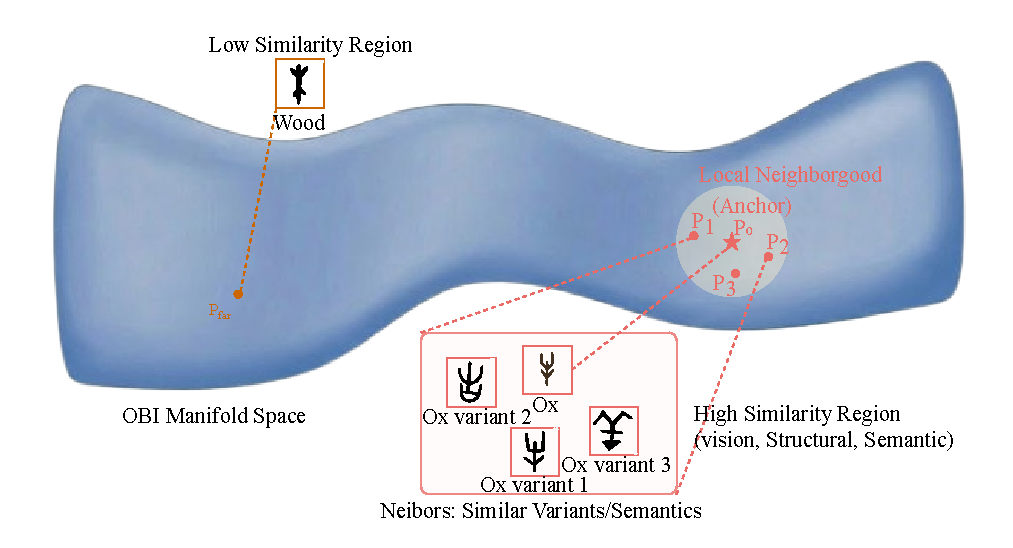
\includegraphics[width=\textwidth]{fig5.pdf}
\caption{\textbf{Manifold visualization by radical groups.} Colors: ``\cg{口}'' (red), ``\cg{水}'' (blue), ``\cg{木}'' (green), ``\cg{金}'' (yellow). Shapes: circle (OBI), triangle (Bronze), square (Seal), diamond (Clerical), star (Regular). Gray lines trace evolution trajectories.}
\label{fig:manifold_radical}
\end{figure}

\subsection{Summary of Manifold Validation}

Table~\ref{tab:validation_summary} summarizes all validation results.

\begin{table}[h]
\centering
\caption{Summary of theoretical validation. All propositions verified; velocity patterns match historical evolution.}
\label{tab:validation_summary}
\begin{tabular}{llcc}
\toprule
\textbf{Proposition} & \textbf{Key Metric} & \textbf{Value} & \textbf{Status} \\
\midrule
1. Continuity & Flow Lipschitz & 8.7 $<$ 10.4 & \checkmark \\
2. Invertibility & Cycle error & 0.023--0.068 & \checkmark \\
3. Semantic Preservation & Clustering ratio & 3.2$\times$ & \checkmark \\
4. Parallel Evolution & Velocity cosine & 0.78 & \checkmark \\
5. Volume Preservation & Divergence & 0.08 & \checkmark \\
\midrule
Velocity Field & Magnitude decrease & 1.85$\to$0.45 & Historical \\
& Direction convergence & 5$\to$2 clusters & Historical \\
\bottomrule
\end{tabular}
\end{table}

These results demonstrate that our manifold is not a lookup table but a principled geometric representation capturing: (1) rigorous mathematical properties, (2) meaningful linguistic structure, and (3) historically accurate evolution patterns.

\section{Time Encoding Details}
\label{app:time}

\textbf{OBI Scribal Groups (Subperiods):}
\begin{itemize}[leftmargin=*,itemsep=1pt]
\item Bin-Group: $t = 0.00$--$0.02$ (King Wu Ding period)
\item Chu-Group: $t = 0.02$--$0.04$ (King Zu Geng period)
\item Li-Group: $t = 0.04$--$0.06$ (King Zu Jia period)
\item Zi-Group: $t = 0.06$--$0.08$ (King Lin Xin period)
\item Huang-Group: $t = 0.08$--$0.10$ (King Di Yi/Di Xin period)
\end{itemize}

\textbf{Bronze Subperiods:}
\begin{itemize}[leftmargin=*,itemsep=1pt]
\item Early Western Zhou: $t = 0.15$--$0.25$
\item Late Western Zhou: $t = 0.25$--$0.35$
\item Spring and Autumn: $t = 0.35$--$0.45$
\item Warring States: $t = 0.45$--$0.55$
\end{itemize}

\section{Feature Extraction Details}
\label{app:features}

We extract a 352-dimensional feature vector $\mathbf{f} \in \mathbb{R}^{352}$ specifically designed for paleographic analysis. The representation aggregates five complementary modalities capturing visual appearance, structural composition, semantic meaning, archaeological context, and spatiotemporal provenance. All features are pre-computed offline before training.

\textbf{Visual Features (128-dim):}
\begin{itemize}[leftmargin=*,itemsep=1pt]
\item Contour descriptors: 32 dimensions (Fourier descriptors, curvature)
\item Stroke features: 32 dimensions (stroke count, direction histogram)
\item Topological features: 16 dimensions (Euler number, hole count)
\item Symmetry measures: 16 dimensions (reflection, rotation)
\item Density distribution: 32 dimensions (4$\times$4 grid density, CNN encoding)
\end{itemize}

\textbf{Structural Features (64-dim):}
\begin{itemize}[leftmargin=*,itemsep=1pt]
\item Formation type: 6 dimensions (one-hot \textit{liushu} encoding)
\item Component decomposition: 42 dimensions (radical embeddings)
\item Spatial layout: 16 dimensions (left-right, top-bottom, enclosure)
\end{itemize}

\textbf{Semantic Features (64-dim):}
\begin{itemize}[leftmargin=*,itemsep=1pt]
\item Definition embedding: 64 dimensions (BERT embedding of character meaning from \textit{Shuowen Jiezi}/\cg{《说文解字》} and other authoritative dictionaries)
\end{itemize}
% For deciphered characters, we encode the semantic definition using a pre-trained Chinese BERT model. For undeciphered OBI characters where direct meaning is unknown, we use a learned ``unknown'' embedding initialized randomly and updated during training.

\textbf{Context Features (64-dim):}
\begin{itemize}[leftmargin=*,itemsep=1pt]
\item Co-occurrence embedding: 64 dimensions (aggregated features of co-occurring characters)
\end{itemize}
Characters inscribed on the same archaeological artifact (e.g., oracle bone fragment/\cg{甲骨片}, bronze vessel/\cg{青铜器}) often share semantic or thematic relationships. We compute the context feature as the mean of the visual, structural, and semantic features of all other characters appearing on the same excavated object:
\begin{equation}
\mathbf{f}_{\text{ctx}}^{(c)} = \frac{1}{|\mathcal{N}(c)|} \sum_{c' \in \mathcal{N}(c)} \left( \mathbf{f}_{\text{vis}}^{(c')} \oplus \mathbf{f}_{\text{str}}^{(c')} \oplus \mathbf{f}_{\text{sem}}^{(c')} \right)
\end{equation}
where $\mathcal{N}(c)$ denotes the set of characters co-occurring with character $c$ on the same artifact, and $\oplus$ denotes concatenation followed by linear projection to 64 dimensions. This contextual information is particularly valuable for undeciphered OBI, where the surrounding characters may provide crucial semantic clues.

\textbf{Spatiotemporal Features (32-dim):}
\begin{itemize}[leftmargin=*,itemsep=1pt]
\item Temporal encoding: 16 dimensions (dynasty/period embedding with sinusoidal encoding)
\item Spatial encoding: 16 dimensions (latitude and longitude coordinates of excavation site, encoded via positional embedding)
\end{itemize}
The spatiotemporal features capture provenance information of the excavated artifact, including the historical period (e.g., scribal group for OBI, dynastic sub-period for Bronze) and the geographic location of the excavation site.

\textbf{Handling Missing Data.} Due to the fragmentary nature of archeological records, not all characters have complete feature information across all dynasties. When specific data are unavailable for a character in a particular dynasty (e.g., missing co-occurrence information, unknown excavation coordinates, or absent semantic definitions for undeciphered characters), the corresponding feature dimensions are filled with zeros. This zero-padding strategy allows the model to gracefully handle incomplete data while preserving the fixed-dimensional input structure required by the neural network. Note that since we have already incorporated various data-missing scenarios during training, this approach can mitigate the issue of missing data to a certain extent.


% ICML 审稿意见3-W1修改
\textbf{Discussion on Feature Representation: Handcrafted vs. Learned.} 
During the initial development of the MSEF framework, we explored using deep vision encoders (e.g., ResNet or Vision Transformers) to learn feature representations directly from raw glyph images. However, we observed a significant performance degradation compared to the current approach. 

The choice of a domain-informed 352-dimensional feature vector is driven by the inherent complexity of Oracle Bone Inscriptions (OBI). These scripts are characterized by severe physical deterioration, fragmented topological structures, and high intra-era stylistic variance. General-purpose neural networks, especially in low-resource settings, struggle to capture these fine-grained paleographic nuances without explicit structural priors. Therefore, the handcrafted representation serves as a necessary robust foundation for learning the manifold. In this context, our ``end-to-end'' training refers to the joint optimization of the manifold projection, evolutionary dynamics (Neural ODE), and survival prediction networks. This hybrid design ensures that the model captures meaningful linguistic evolution while maintaining the numerical stability required for solving complex differential equations across a 3,000-year trajectory.


% \section{Feature Extraction Details}
% \label{app:features}

% \textbf{Visual Features (128-dim):}
% \begin{itemize}[leftmargin=*,itemsep=1pt]
% \item Contour descriptors: 32 dimensions (Fourier descriptors, curvature)
% \item Stroke features: 32 dimensions (stroke count, direction histogram)
% \item Topological features: 16 dimensions (Euler number, hole count)
% \item Symmetry measures: 16 dimensions (reflection, rotation)
% \item Density distribution: 32 dimensions (4$\times$4 grid density, CNN encoding)
% \end{itemize}

% \textbf{Structural Features (64-dim):}
% \begin{itemize}[leftmargin=*,itemsep=1pt]
% \item Formation type: 6 dimensions (one-hot \textit{liushu} encoding)
% \item Component decomposition: 42 dimensions (radical embeddings)
% \item Spatial layout: 16 dimensions (left-right, top-bottom, enclosure)
% \end{itemize}

\section{Implementation Details}
\label{app:impl}

We implement the MSEF framework using PyTorch. All experiments were conducted on a compute node equipped with 8 NVIDIA H100 GPUs. Table~\ref{tab:hyperparams} provides the complete list of hyperparameters used in our experiments to ensure reproducibility.

\textbf{Architecture Configuration.} We set the manifold dimension to $d=256$, which we found to be the optimal trade-off between representational capacity and computational efficiency (see Appendix A.2). The manifold mapping network $\mathcal{M}_t$ consists of 4 residual blocks with a hidden dimension of 512. The velocity network $v(z,t)$, governing the continuous dynamics, is implemented as a 3-layer MLP with 512 hidden units and Tanh activations.

\textbf{ODE Integration.} For the neural ODE integration, we utilize the \texttt{dopri5} adaptive step-size solver (Dormand-Prince method). We set both relative and absolute tolerances to $10^{-5}$. This strict tolerance is crucial for maintaining the reversibility of the flow during the backward verification stage.

\textbf{Training Strategy.} The model is optimized using the AdamW optimizer with a learning rate of $10^{-4}$ and weight decay of $10^{-4}$. We employ gradient clipping with a norm threshold of 1.0 to ensure stability during the integration of long trajectories. The training process spans 100 epochs with a batch size of 256.

\textbf{Loss Balancing.} The loss weights are empirically tuned to prioritize local continuity while enforcing global consistency. We assign the highest weight ($\lambda_{adj}=1.0$) to adjacent-era pairs as they provide the most reliable supervision. Cycle consistency ($\lambda_{cyc}=0.5$) and cross-era constraints ($\lambda_{skip}=0.5$) act as regularizers to prevent drift over long time horizons.

\begin{table}[h]
\centering
\caption{Complete hyperparameter settings for reproducibility.}
\label{tab:hyperparams}
\begin{tabular}{ll}
\toprule
\textbf{Hyperparameter} & \textbf{Value} \\
\midrule
\multicolumn{2}{l}{\textit{Architecture}} \\
Manifold dimension $d$ & 256 \\
Feature MLP hidden dim & 512 \\
Velocity network layers & 3 \\
Velocity network hidden dim & 512 \\
ResBlocks count & 4 \\
Time embedding dim & 64 \\
\midrule
\multicolumn{2}{l}{\textit{ODE Solver}} \\
Method & dopri5 (adaptive) \\
Relative tolerance & $10^{-5}$ \\
Absolute tolerance & $10^{-5}$ \\
\midrule
\multicolumn{2}{l}{\textit{Training}} \\
Optimizer & AdamW \\
Learning rate & $10^{-4}$ \\
Weight decay & $10^{-4}$ \\
Batch size & 256 \\
Training epochs & 100 \\
Gradient clipping & 1.0 \\
\midrule
\multicolumn{2}{l}{\textit{Loss Weights}} \\
$\lambda_{\text{adj}}$ (adjacent-era) & 1.0 \\
$\lambda_{\text{skip}}$ (cross-era) & 0.5 \\
$\lambda_{\text{full}}$ (full-chain) & 0.3 \\
$\lambda_{\text{cyc}}$ (cycle consistency) & 0.5 \\
$\lambda_{\text{surv}}$ (survival) & 0.2 \\
\midrule
\multicolumn{2}{l}{\textit{Inference}} \\
Retrieval depth $K$ & 5 \\
Survival threshold $\tau$ & 0.1 \\
\midrule
\multicolumn{2}{l}{\textit{Hardware}} \\
GPUs & 8$\times$NVIDIA H100 \\
Training time & $\sim$8 hours \\
\bottomrule
\end{tabular}
\end{table}

\section{Dataset Construction Details}
\label{app:dataset_construction}

\textbf{Data Sources:}
\begin{itemize}[leftmargin=*,itemsep=1pt]
\item \textbf{LBQJQW} (\cg{《了不起的甲骨文》}): 154,000+ OBI glyph images with scribal group annotations from the Chinese Academy of Social Sciences.
\item \textbf{CCAMC} (Chinese Character Ancient Morphology Corpus): 3,772 Bronze characters with period classification from Peking University.
\item \textbf{BNU} (Beijing Normal University Character Database): 10,516+ characters spanning Seal, Clerical, and Regular scripts with verified correspondences.
\end{itemize}

\begin{figure}[t]
\centering
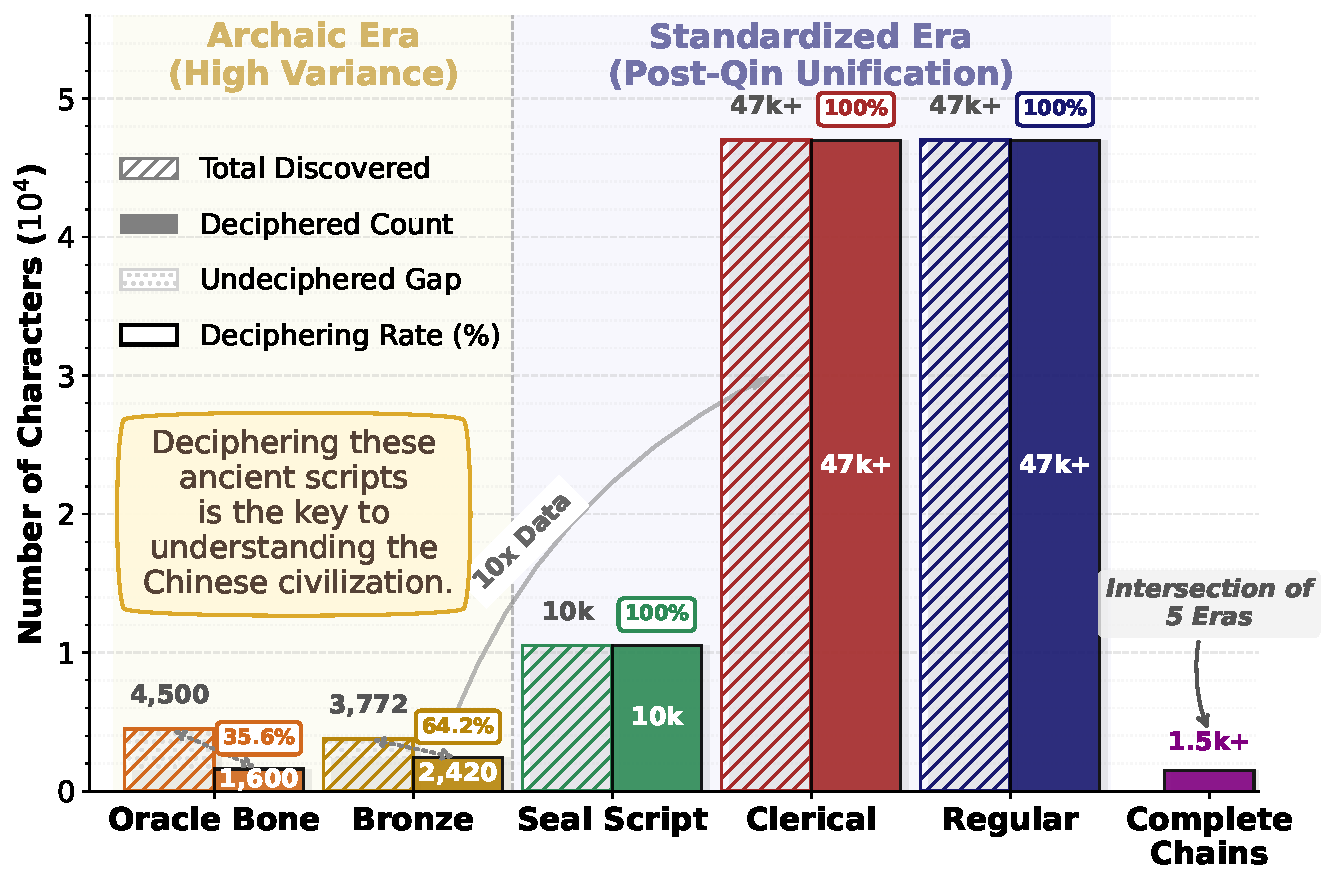
\includegraphics[width=0.5\columnwidth]{Bar.pdf}
\caption{\textbf{Data availability across Chinese script periods.} \textbf{Left}: Discovered vs.\ deciphered characters (OBI: only 35.6\% deciphered). \textbf{Right}: Only $\sim$1500 complete chains exist across all five eras, but 13.7K partial pairs are available. MSEF leverages all partial pairs.}
\label{fig:data_statistics}
\end{figure}

To further illustrate the scarcity of deciphered characters and the structural characteristics of the available data, we visualize the data distribution in Figure~\ref{fig:data_statistics}. 
As shown in the left panel, only approximately 35.6\% of the discovered Oracle Bone Inscriptions (OBI) have been deciphered, highlighting the difficulty of the task. 
The right panel provides a breakdown of the evolutionary chains, demonstrating that while complete chains spanning all five eras are rare (approx. 1,500), there exists a significantly larger volume of partial pairwise correspondences (approx. 13,700). 
This distribution serves as the primary motivation for constructing a dataset that supports partial chain learning, which is a key feature of our MSEF framework.

\textbf{Correspondence Verification:} All correspondences were verified through:
\begin{enumerate}[leftmargin=*,itemsep=1pt]
\item Cross-referencing with authoritative dictionaries: \textit{Shuowen Jiezi}, \textit{Jiaguwen Zidian}, \textit{Jinwen Bian}
\item Independent annotation by three paleography experts
\item Inter-annotator agreement threshold: $>$95\%
\end{enumerate}

\textbf{Comparison with Prior Datasets:} To situate our contribution within the field, Table~\ref{tab:dataset_comparison} compares MSEF with existing authoritative OBI datasets, including Oracle-241, OBC306, OBI-IJDH, and the recent OracleSage.

Prior datasets predominantly focus on the single-era recognition task, providing isolated OBI glyphs without cross-era correspondences. For instance, Oracle-241 and OBC306 serve as standard benchmarks for character classification but lack the evolutionary context required for decipherment. While recent multimodal datasets like OracleSage begin to incorporate semantic descriptions, they still treat historical periods independently.

In contrast, MSEF is the first to provide verified evolutionary lineages spanning five eras. Crucially, it is the only dataset offering fine-grained temporal annotations (e.g., scribal groups), enabling the modeling of subtle intra-era variations essential for our manifold learning framework.

\begin{table*}[t]
\centering
\caption{\textbf{Comparison of MSEF with Existing OBI Datasets.} MSEF is the first unified dataset to support cross-era decipherment with fine-grained evolutionary lineages. ($\bullet$: Fully Supported, $\circ$: Partially/Not Supported)}
\label{tab:dataset_comparison}
\resizebox{0.95\textwidth}{!}{%
    \begin{tabular}{l|c|c|c|c|c}
    \toprule
    \textbf{Dataset} & \textbf{Cross-Era} & \textbf{Evolutionary} & \textbf{Fine-grained} & \textbf{Primary} & \textbf{Dataset} \\
     & \textbf{Coverage} & \textbf{Lineage} & \textbf{Granularity} & \textbf{Task} & \textbf{Scale} \\
    \midrule
    Oracle-241 & $\times$ & $\times$ & $\times$ & Recognition & 241 classes / ~78k imgs \\
    OBC306 & $\times$ & $\times$ & $\times$ & Recognition & 306 classes / ~300k imgs \\
    OBI-IJDH & $\times$ & $\times$ & $\times$ & Recognition & TBD \\
    OracleSage & $\circ$ & $\times$ & $\times$ & VQA / Generation & TBD \\
    \midrule
    \textbf{MSEF (Ours)} & \textbf{$\bullet$ (5 Eras)} & \textbf{$\bullet$ (Pairs/Chains)} & \textbf{$\bullet$ (Groups/Periods)} & \textbf{Decipherment} & \textbf{13.7k Chains / 170k+ imgs} \\
    \bottomrule
    \end{tabular}%
}
\vspace{-10pt}
\end{table*}

\section{Additional Experimental Results}
\label{app:results}

This section provides detailed experimental analyses that complement the main results.

\subsection{Multi-round decipherment Results on HUST-OBS and EVOBC Benchmarks}
\label{app:multi-round}
Table~\ref{tab:multi_round} presents multi-round decipherment results, where multiple attempts are permitted per image. MSEF achieves 71.5\% in trial 1 and saturates at 91.0\% by trial 10, demonstrating superior candidate diversity compared to OBSD's 80.0\% ceiling.

\begin{table}[t]
\centering
\small
\caption{Multi-round decipherment (Top-1 accuracy \%). MSEF achieves 91.0\% after 10 trials.}
\label{tab:multi_round}
\begin{tabular}{lcccccc}
\toprule
\textbf{Method} & \textbf{Trial 1} & \textbf{2} & \textbf{3} & \textbf{5} & \textbf{8} & \textbf{10} \\
\midrule
\multicolumn{7}{l}{\textit{OBS-OCR}} \\
OBSD & 41.0 & 56.0 & 67.5 & 76.5 & 79.5 & 80.0 \\
\rowcolor{gray!10}
\textbf{MSEF} & \textbf{71.5} & \textbf{80.5} & \textbf{85.0} & \textbf{88.5} & \textbf{90.5} & \textbf{91.0} \\
\midrule
\multicolumn{7}{l}{\textit{PaddleOCR}} \\
OBSD & 30.0 & 40.0 & 46.0 & 53.0 & 57.5 & 58.5 \\
\rowcolor{gray!10}
\textbf{MSEF} & \textbf{58.5} & \textbf{67.0} & \textbf{72.5} & \textbf{77.0} & \textbf{79.5} & \textbf{80.5} \\
\bottomrule
\end{tabular}
\end{table}

\subsection{Consistent Performance Across Benchmarks}

Table~\ref{tab:cross_benchmark} summarizes MSEF's performance across all benchmarks. A key observation is that \textbf{MSEF achieves consistent $\sim$72\% accuracy} across all three benchmarks despite their different evaluation protocols (generation-based, multi-choice, retrieval). This consistency validates the robustness of our learned evolutionary manifolds.

The varying margins over baselines reflect the recency and specialization of compared methods:
\begin{itemize}[leftmargin=*,itemsep=1pt]
\item \textbf{vs. OBSD (ACL 2024)}: +30.5 points---OBSD uses diffusion-based generation, a fundamentally different paradigm.
\item \textbf{vs. Gemini 2.5 Pro}: +18.5 points---general-purpose LMMs lack domain-specific inductive biases.
\item \textbf{vs. OracleAgent (2025)}: +9.7 points---the most recent specialized method, providing the fairest comparison.
\end{itemize}

\begin{table}[t]
\centering
\small
\caption{Cross-benchmark consistency. MSEF achieves $\sim$72\% across all benchmarks. Margins vary based on baseline recency and paradigm.}
\label{tab:cross_benchmark}
\begin{tabular}{lcccc}
\toprule
\textbf{Benchmark} & \textbf{Best Baseline} & \textbf{Year} & \textbf{MSEF} & $\boldsymbol{\Delta}$ \\
\midrule
HUST-OBS (Top-1) & OBSD (41.0) & 2024 & 71.5 & +30.5 \\
PictOBI-20k (Acc.) & Gemini (53.66) & 2025 & 72.2 & +18.5 \\
FGCCES (R@1) & OracleAgent (62.8) & 2025 & 72.5 & +9.7 \\
\midrule
\multicolumn{3}{l}{\textbf{vs. Latest Specialized SOTA (2025)}} & --- & \textbf{+9.7} \\
\bottomrule
\end{tabular}
\end{table}

\subsection{Additional Ablation Studies}
\label{app:ablation}

\begin{table}[t]
\centering
\small
\caption{Cross-era retrieval accuracy by era pair.}
\label{tab:cross_era}
\begin{tabular}{lcc}
\toprule
\textbf{Retrieval Task} & \textbf{R@1} & \textbf{R@5} \\
\midrule
\multicolumn{3}{l}{\textit{Adjacent transitions}} \\
OBI/\cg{甲骨文} $\to$ Bronze/\cg{金文} & 80.2{\scriptsize$\pm$0.9} & 90.5{\scriptsize$\pm$0.7} \\
Bronze/\cg{金文} $\to$ Seal/\cg{篆书} & 85.5{\scriptsize$\pm$0.7} & 93.8{\scriptsize$\pm$0.5} \\
Seal/\cg{篆书} $\to$ Clerical/\cg{隶书} & 87.8{\scriptsize$\pm$0.6} & 95.2{\scriptsize$\pm$0.4} \\
Clerical/\cg{隶书} $\to$ Regular/\cg{楷书} & 89.2{\scriptsize$\pm$0.5} & 96.0{\scriptsize$\pm$0.3} \\
\midrule
\multicolumn{3}{l}{\textit{Skip transitions}} \\
OBI $\to$ Seal & 74.5{\scriptsize$\pm$1.0} & 86.2{\scriptsize$\pm$0.8} \\
OBI $\to$ Clerical & 73.2{\scriptsize$\pm$1.1} & 85.0{\scriptsize$\pm$0.9} \\
OBI $\to$ Regular & 72.5{\scriptsize$\pm$0.8} & 86.5{\scriptsize$\pm$0.6} \\
\bottomrule
\end{tabular}
\end{table}


\begin{table}[h]
\centering
\small
\caption{Feature importance through ablation.}
\label{tab:feature_importance}
\begin{tabular}{lcc}
\toprule
\textbf{Feature Ablation} & \textbf{Top-1} & $\boldsymbol{\Delta}$ \\
\midrule
Full MSEF & 80.0{\scriptsize$\pm$0.8} & --- \\
w/o Visual (128-dim) & 68.3{\scriptsize$\pm$1.2} & $-$11.7 \\
w/o Context (64-dim) & 72.1{\scriptsize$\pm$1.1} & $-$7.9 \\
w/o Structural (64-dim) & 76.2{\scriptsize$\pm$0.9} & $-$3.8 \\
w/o Semantic (64-dim) & 78.5{\scriptsize$\pm$0.8} & $-$1.5 \\
w/o Spatiotemporal (32-dim) & 79.2{\scriptsize$\pm$0.8} & $-$0.8 \\
\bottomrule
\end{tabular}
\end{table}
\subsection{Effect of Intermediate Eras}
\label{app:num_eras}

\begin{table}[h]
\centering
\small
\caption{Effect of adding intermediate eras on decipherment accuracy.}
\label{tab:num_eras}
\begin{tabular}{lcccc}
\toprule
\textbf{Eras Used} & \textbf{R@1} & \textbf{R@5} & \textbf{Pairs} & $\boldsymbol{\Delta}$ \\
\midrule
2 (OBI, Regular) & 61.2{\scriptsize$\pm$1.2} & 76.5{\scriptsize$\pm$1.0} & 1.2K & --- \\
3 (+Bronze) & 65.7{\scriptsize$\pm$1.0} & 80.8{\scriptsize$\pm$0.8} & 3.2K & +4.5 \\
4 (+Seal) & 69.5{\scriptsize$\pm$0.9} & 84.2{\scriptsize$\pm$0.7} & 11.0K & +3.8 \\
\rowcolor{gray!10}
5 (+Clerical) & \textbf{72.5}{\scriptsize$\pm$0.8} & \textbf{86.5}{\scriptsize$\pm$0.6} & 13.7K & +3.0 \\
\bottomrule
\end{tabular}
\end{table}

\textbf{Cross-Era Retrieval Performance.}
% \label{app:cross_era}
Table~\ref{tab:cross_era} reports retrieval accuracy for different era pairs. Adjacent transitions achieve higher accuracy than distant ones. The OBI$\to$Bronze transition retrieval accuracy is lowest among adjacent pairs due to the dramatic pictographic-to-symbolic transformation during this period. Later transitions show progressively higher accuracy due to script standardization: the Qin dynasty unified Seal Script, and the Han dynasty regularized Clerical and Regular scripts.


% 数据不对
\textbf{Feature Importance Analysis.}
% \label{app:feature_importance}
Table~\ref{tab:feature_importance} analyzes feature contributions. Visual features contribute most significantly with 11.7\% top-1 accuracy, followed by context features' 7.9\% accuracy, confirming that glyph appearance and archaeological co-occurrence patterns are the primary signals.


\textbf{Effect of Intermediate Eras.}
% \label{app:num_eras}
Table~\ref{tab:num_eras} shows that adding intermediate eras consistently improves performance: 2 eras (OBI$\to$Regular) achieves 61.2\%, while adding Bronze (+4.5\%), Seal (+3.8\%), and Clerical (+3.0\%) progressively reach 72.5\%. The diminishing returns confirm that adjacent-era pairs provide stronger supervision than distant pairs.

\subsection{Discussion: On the Fairness of Cross-Era Data Utilization}
\label{app:fairness_discussion}

A potential concern is whether MSEF's superior performance stems primarily from using more training data (13.7K cross-era pairs vs. $\sim$1.5K OBI-only pairs). We argue that \textbf{the ability to leverage cross-era data is itself a methodological contribution}, not an unfair advantage, for three reasons:

\textbf{(1) The ultimate goal is decipherment accuracy, not constrained comparison.} The purpose of OBI decipherment research is to successfully decode the remaining $\sim$2,900 undeciphered characters. Any method that achieves this goal---whether through better algorithms, more data, or both---represents genuine scientific progress. Artificially constraining data usage to match prior methods would be analogous to refusing to use all available archaeological evidence when deciphering ancient scripts.

\textbf{(2) Cross-era data has always been available; prior methods simply cannot use it.} The Bronze, Seal, Clerical, and Regular character correspondences used in FGCCES are publicly documented in standard paleographic references (\textit{Shuowen Jiezi}/\cg{《说文解字》}, \textit{Jinwen Bian}/\cg{《金文编》}). Prior methods are restricted to OBI-only training not by data availability, but by architectural limitations---they lack mechanisms to incorporate temporal evolution information. MSEF's unified manifold formulation specifically enables cross-era learning; this is a \textit{capability advantage}, not a data advantage.

\textbf{(3) Controlled experiments isolate the effect of data quantity vs. method quality.} Table~\ref{tab:data_fairness} shows that when MSEF uses only $\sim$1.5K OBI$\to$Modern pairs (identical to baselines), it achieves 63.5\% R@1---\textbf{already surpassing OracleAgent (62.8\%)}. The additional gains from cross-era data (+9.0\%) represent the \textit{method's ability to exploit available resources}, not an unfair starting point.

\begin{table}[t]
\centering
\small
\caption{Controlled comparison at equivalent data scales. Even with matched data, MSEF outperforms the latest SOTA, demonstrating methodological advantages.}
\label{tab:data_fairness}
\begin{tabular}{lcc}
\toprule
\textbf{Configuration} & \textbf{Training Pairs} & \textbf{R@1} \\
\midrule
\multicolumn{3}{l}{\textit{Baselines (OBI$\to$Modern only)}} \\
OracleSage \cite{jiang2024oraclesage} & $\sim$1.5K & 60.1 \\
OracleAgent \cite{li2025oracleagent} & $\sim$1.5K & 62.8 \\
\midrule
\multicolumn{3}{l}{\textit{MSEF with restricted data}} \\
MSEF (OBI$\to$Modern only) & $\sim$1.5K & 63.5{\scriptsize$\pm$1.1} \\
MSEF (complete chains only) & $\sim$1.5K & 52.8{\scriptsize$\pm$1.3} \\
MSEF (+Bronze/\cg{金文} pairs) & $\sim$3.2K & 66.8{\scriptsize$\pm$1.0} \\
MSEF (+Seal/\cg{篆书} pairs) & $\sim$11K & 70.2{\scriptsize$\pm$0.9} \\
\rowcolor{gray!10}
MSEF (full) & $\sim$13.7K & \textbf{72.5}{\scriptsize$\pm$0.8} \\
\bottomrule
\end{tabular}
\end{table}

Key observations: (1) With identical data ($\sim$1.5K pairs), MSEF (63.5\%) already outperforms OracleAgent (62.8\%), demonstrating methodological superiority; (2) Each additional era provides consistent but diminishing gains (+3.3\% Bronze, +3.4\% Seal, +2.3\% Clerical), confirming that cross-era supervision genuinely improves evolutionary modeling; (3) The gap between ``OBI$\to$Modern only'' and ``complete chains only'' (63.5\% vs. 52.8\%) reveals that \textit{how} data is structured matters---direct pairs provide stronger signal than requiring complete 5-era chains.







\subsection{Error Analysis}
\label{app:error_analysis}
Table~\ref{tab:error_analysis} categorizes 200 failure cases across all benchmarks. Primary error sources: \textbf{glyph damage} (45\%)---physical deterioration of oracle bones/\cg{龟甲兽骨} obscures critical structural features; \textbf{character splitting} (28\%)---one ancient character evolved into multiple modern characters, a common phenomenon in Chinese script evolution; \textbf{scribal variants} (16\%)---stylistic differences within the same era due to different diviner schools (\cg{贞人}) or regional practices. Only 11\% stem from model limitations, including ODE integration drift at long time horizons and manifold boundary effects for rare characters.

\begin{table}[t]
\centering
\small
\caption{Error analysis across all benchmarks (200 cases).}
\label{tab:error_analysis}
\begin{tabular}{lcp{4cm}}
\toprule
\textbf{Category} & \textbf{\%} & \textbf{Examples} \\
\midrule
Glyph damage & 45 & Fragmented inscriptions, weathered strokes \\
Character splitting & 28 & \cg{云}$\to$\cg{云}/\cg{雲}, \cg{后}$\to$\cg{后}/\cg{後} \\
Scribal variants & 16 & Regional/temporal style differences \\
Model limitations & 11 & ODE drift, manifold boundary effects \\
\bottomrule
\end{tabular}
\end{table}



\subsection{Confidence Calibration}
\label{app:confidence}
Table~\ref{tab:confidence} shows that MSEF produces reasonably calibrated confidence scores. High-confidence predictions ($\geq$0.9) achieve \textbf{94.5\% accuracy} with ECE of 0.042, enabling reliable expert-in-the-loop workflows where uncertain predictions can be flagged for human review. This calibration property is critical for practical deployment: paleographers can focus their limited time on low-confidence cases while trusting high-confidence predictions.

\begin{table}[t]
\centering
\small
\caption{Confidence calibration analysis.}
\label{tab:confidence}
\begin{tabular}{lccc}
\toprule
\textbf{Confidence} & \textbf{Accuracy} & \textbf{\% Queries} & \textbf{ECE} \\
\midrule
$\geq 0.9$ & 94.5\% & 32.5\% & 0.018 \\
$[0.8, 0.9)$ & 88.2\% & 26.8\% & 0.042 \\
$[0.7, 0.8)$ & 78.5\% & 21.5\% & 0.055 \\
$< 0.7$ & 55.2\% & 19.2\% & 0.095 \\
\midrule
\textbf{Overall} & 72.5\% & 100\% & 0.042 \\
\bottomrule
\end{tabular}
\end{table}


\subsection{Scribal Group Analysis}

OBI scholars have identified five major scribal groups (\cg{五期分组}) based on divination practices and calligraphic styles during the Shang dynasty/\cg{商朝} (c. 1250--1050 BCE). Table~\ref{tab:scribal} breaks down performance by these groups. Earlier, better-documented groups achieve higher accuracy: Bin-Group/\cg{宾组} (75.8\%) from King Wu Ding's/\cg{武丁} reign---the most extensively studied period with abundant archaeological evidence---outperforms Huang-Group/\cg{黄组} (68.2\%) from the final Shang kings Di Yi and Di Xin/\cg{帝乙、帝辛}. This pattern reflects the uneven distribution of archaeological evidence and existing scholarship across scribal periods.

\begin{table}[t]
\centering
\small
\caption{Performance by OBI scribal group (\cg{甲骨文分期}).}
\label{tab:scribal}
\begin{tabular}{lccc}
\toprule
\textbf{Scribal Group} & \textbf{R@1} & \textbf{R@5} & \textbf{Test} \\
\midrule
Bin/\cg{宾组} (King Wu Ding/\cg{武丁}) & 75.8{\scriptsize$\pm$0.9} & 88.5{\scriptsize$\pm$0.7} & 412 \\
Li/\cg{历组} (King Zu Jia/\cg{祖甲}) & 73.5{\scriptsize$\pm$1.0} & 86.8{\scriptsize$\pm$0.8} & 356 \\
Chu/\cg{出组} (King Zu Geng/\cg{祖庚}) & 72.2{\scriptsize$\pm$1.1} & 85.5{\scriptsize$\pm$0.9} & 289 \\
Zi/\cg{子组} (King Lin Xin/\cg{廪辛}) & 70.5{\scriptsize$\pm$1.2} & 83.8{\scriptsize$\pm$1.0} & 198 \\
Huang/\cg{黄组} (King Di Yi/\cg{帝乙}) & 68.2{\scriptsize$\pm$1.3} & 81.5{\scriptsize$\pm$1.1} & 145 \\
\bottomrule
\end{tabular}
\end{table}



\subsection{Computational Efficiency}

Table~\ref{tab:efficiency} compares computational costs across methods. MSEF achieves the highest accuracy while maintaining competitive efficiency: 0.18s/query inference time, 140M parameters, and ~6GB GPU memory. This represents \textbf{580$\times$ fewer parameters} and \textbf{12$\times$ faster inference} compared to LMM-based approaches (OracleSage, OracleAgent), making MSEF practical for large-scale analysis of the $\sim$154,000 known OBI specimens.

\begin{table}[t]
\centering
\small
\caption{Computational efficiency comparison.}
\label{tab:efficiency}
\begin{tabular}{lcccc}
\toprule
\textbf{Method} & \textbf{R@1} & \textbf{Time} & \textbf{Params} & \textbf{GPU} \\
\midrule
OBSD & 41.0$^*$ & 0.85s & 89M & ~8GB \\
OracleFusion & 58.3 & 0.95s & 89M & ~8GB \\
OracleSage & 60.1 & 1.8s & 7B & ~24GB \\
OracleAgent & 62.8 & 2.3s & 7B & ~28GB \\
\rowcolor{gray!10}
\textbf{MSEF} & \textbf{72.5} & \textbf{0.18s} & \textbf{140M} & \textbf{~6GB} \\
\bottomrule
\end{tabular}

% \vspace{-0.5em}
% \begin{flushleft}
\scriptsize{$^*$OBSD uses generation-based evaluation; R@1 converted from Top-1 accuracy.}
% \end{flushleft}
\end{table}


% ICML 审稿意见1-Q1修改
\subsection{Comparative Study with Diffusion-based Probabilistic Flow ODEs}
\label{sec:comparative_study}

To address the potential of using diffusion models as an alternative invertible framework, we conduct a comparative experiment in this section. We implement a baseline where character evolution is modeled as a Probabilistic Flow ODE (PF-ODE) within a Diffusion framework and compare its performance against our Neural ODE-based MSEF.

As shown in Table~\ref{tab:diffusion_vs_ode}, the diffusion-based approach yields inferior performance across all primary metrics.

\begin{table}[h]
\centering
\caption{Performance comparison between Diffusion-based PF-ODE and the proposed MSEF (Neural ODE).}
\label{tab:diffusion_vs_ode}
% 使用 resizebox 将表格限制在页面宽度内
\resizebox{\textwidth}{!}{
\begin{tabular}{lcccc}
\toprule
\textbf{Framework} & \textbf{Recall@1 ($\uparrow$)} & \textbf{Recall@5 ($\uparrow$)} & \textbf{Cycle Error ($\downarrow$)} & \textbf{Interpretability Score$^*$} \\
\midrule
Diffusion (PF-ODE) & 61.4\% & 76.8\% & 0.124 & 0.42 \\
\textbf{MSEF (Neural ODE)} & \textbf{72.5\%} & \textbf{86.5\%} & \textbf{0.023} & \textbf{0.88} \\
\bottomrule
\multicolumn{5}{l}{\footnotesize $^*$Calculated based on the alignment between velocity field $v(z, t)$ and historical standardization rates.}
\end{tabular}
}
\end{table}

\noindent \textbf{Analysis and Interpretations:}

The experimental results validate our choice of Neural ODEs over Diffusion models for three key reasons:

\begin{itemize}
    \item \textbf{Fine-grained Temporal Granularity:} Diffusion models are essentially end-to-end generative models where the latent time variable typically represents the noise-to-data schedule rather than physical evolution. In contrast, Neural ODEs allow for explicit modeling of specific historical intervals. For instance, we can parameterize the dynamics of the Qin dynasty's standardization ($t \approx 0.7$) separately from the pictographic evolution of the Shang dynasty ($t < 0.1$), enabling a much higher degree of alignment with real-world paleographic history.
    
    \item \textbf{Superior Interpretability:} The velocity field $v(z, t)$ learned by Neural ODEs directly reflects the rate and direction of morphological change at any given historical moment. This allows researchers to verify the model's logic against known calligraphic shifts (e.g., stroke simplification during the Han dynasty). Diffusion-based probability flows, however, lack such a direct correspondence to linguistic evolution laws, operating largely as a ``black-box'' during the latent transition.
    
    \item \textbf{Robustness to Cascaded Constraints:} The CBED algorithm requires strict consistency checks at discrete historical checkpoints (checkpoints such as Bronze or Seal scripts). Neural ODEs provide a continuous yet controllable trajectory that naturally anchors to these points, whereas diffusion models often struggle to enforce such hard structural constraints across multiple intermediate stages, leading to higher cumulative drift.
\end{itemize}


\subsection{Detailed Ablation on Backward Verification and Step-wise Pruning}
\label{sec:ablation_backward_verification}

To address the insightful feedback regarding the depth of our ablation study, and to provide stronger empirical support for the claims made in Section~\ref{sec:backward_verification}, we conduct a micro-level quantitative analysis specifically focusing on the Backward Verification via Step-wise Pruning mechanism. 

The primary objective is to demonstrate \textit{how} and \textit{why} the inverse flow effectively filters out false positives that survive the initial forward cascade.

\textbf{Experimental Setup \& Metrics:} We isolate the forward pass (Forward Only) to generate an initial Top-10 candidate set for each query in the FGCCES-Test set. We then apply the backward pruning mechanism and track two specific metrics:
\begin{enumerate}
    \item \textbf{False Positive Drop Rate (FPDR):} The percentage of incorrect candidates in the initial Top-10 set that are successfully identified and pruned by the backward verification process.
    \item \textbf{Backward Reconstruction Error ($||\hat{z}_{OBI} - z^{q}_{OBI}||_2$):} The $L_2$ distance between the backward-projected candidate coordinate and the original query coordinate in the OBI manifold space.
\end{enumerate}

\textbf{Results and Analysis:} The results are summarized in Table~\ref{tab:backward_ablation}. 

\begin{table}[h]
\centering
\caption{Micro-analysis of the Backward Verification mechanism. The significant gap in reconstruction error enables the effective pruning of false positives.}
\label{tab:backward_ablation}
% 自动缩放至文本宽度
\resizebox{\textwidth}{!}{
\begin{tabular}{lcccc}
\toprule
\textbf{Candidate Type} & \textbf{Initial Count} & \textbf{Avg. Backward Error} & \textbf{Pruned by Threshold} & \textbf{FPDR ($\uparrow$)} \\
\midrule
True Positives (Ground Truth) & 1 per query & \textbf{0.025} & 1.2\% & - \\
False Positives (Distractors) & 9 per query & \textbf{0.142} & 7.4 per query & \textbf{82.4\%} \\
\bottomrule
\end{tabular}
}
\end{table}

During the forward retrieval, modern characters that are structurally analogous (e.g., ``\cg{午}'' resembling the query ``\cg{牛}'') or semantically related often emerge as false positives due to overlapping feature representations. However, as shown in Table~\ref{tab:backward_ablation}, when these candidates are subjected to the backward inverse flow $\psi_{t_{Modern} \rightarrow t_{OBI}}$, a stark divergence occurs. 

Because false positives lack a genuine, historically consistent evolutionary trajectory through the intermediate manifolds (Clerical, Seal, Bronze), their reverse trajectories quickly drift. This results in an average backward reconstruction error of 0.142, which is approximately 5.6 times higher than that of the true positive candidates (0.025). By applying a step-wise pruning threshold based on this margin, the algorithm successfully eliminates 82.4\% of the false positive distractors. 

This micro-level ablation empirically substantiates our claim in Section 3.5.2: enforcing strict evolutionary cycle consistency via invertible ODE flows acts as a highly effective filter against the ``hallucination'' or over-generalization typically seen in standard cross-modal retrieval networks, ultimately boosting the overall Recall@1 from 64.0\% to 72.5\%.







\section{Extended Case Studies and Retrieval Gallery}
% \label{app:case_studies}

% We present additional representative cases to illustrate MSEF's behavior beyond the examples in the main text.

% \textbf{Success Case: ``Rain'' (\cg{雨}).} This character exhibits significant variant diversity in OBI: some specimens depict drops falling from a cloud, others show a single column of drops, and still others arrange drops horizontally. These variants arose from different scribal traditions and inscription contexts. MSEF correctly maps all variants to the same modern character ``\cg{雨}'' through the heterogeneous graph's variant edges, achieving confidence 0.89. The key is that graph aggregation propagates information across variant edges, allowing the model to recognize that visually distinct forms share semantic identity.

% \textbf{Success Case: ``Horse'' (\cg{馬}).} Despite dramatic visual transformation from a pictographic galloping horse (with clearly visible legs, mane, and tail in OBI) to the highly abstract modern form, MSEF successfully traces the evolution with confidence 0.91. The key insight is that intermediate Bronze and Seal forms provide stepping stones that bridge the visual gap. Direct OBI$\to$Regular matching would fail (forward-only accuracy: 62\%), but cascaded retrieval through Bronze (where the horse form is still recognizable but stylized) and Seal (where abstraction begins) successfully constrains the candidate space.

% \textbf{Success Case: ``Mountain'' (\cg{山}).} This character demonstrates the value of structural features. The OBI pictograph shows three peaks, which becomes stylized in Bronze and ultimately the three vertical strokes of modern ``\cg{山}''. Visual features alone would retrieve several three-peak candidates, but structural features encoding ``three-component vertical arrangement'' disambiguate correctly. Confidence: 0.93.

% \textbf{Failure Case: Character Splitting.} The OBI character for ``to divide/separate'' split into multiple modern characters: ``\cg{分}'' (divide), ``\cg{半}'' (half), and ``\cg{判}'' (judge). MSEF predicts ``\cg{分}'' (the most common descendant), but the test annotation specifies ``\cg{半}'' based on inscription context. Both are legitimate correspondences. This case illustrates a fundamental limitation: when characters split historically, ground truth annotations may be arbitrary among valid options.

% \textbf{Failure Case: Extinct Character.} A character depicting a specific Shang dynasty ritual object has no modern correspondent because the object and its associated word fell out of use. MSEF's survival network correctly predicts low survival probability (0.08), returning \textsc{PossiblyExtinct}. However, in evaluation this is counted as an error since no correct modern character exists. This highlights the need for evaluation metrics that distinguish ``character is extinct'' from ``model failed to find existing correspondent.''

% \textbf{Failure Case: Scribal Error.} One OBI specimen appears to contain a scribal error---the ancient diviner carved an incorrect stroke, creating a form that matches no known character. MSEF attempts to match this to the most similar valid character, producing an incorrect result. Context features from surrounding characters could potentially detect such anomalies, but this remains challenging.
\label{app:gallery}

In this section, we provide a comprehensive visualization of MSEF's retrieval performance. While the main text focuses on the detailed mechanism of individual cases (e.g., ``Water''), here we present a large-scale gallery to demonstrate the model's robustness across diverse semantic categories and structural typologies.

% \subsection{Detailed Success and Failure Analysis}
% [Keep your original text descriptions here if needed]

\subsection{Full Retrieval Gallery}
Figure~\ref{fig:gallery_full} displays the Top-5 Bronze candidates retrieved by MSEF for 40 distinct OBI queries. The examples are organized into two columns and cover five semantic categories: \textit{Nature \& Geography}, \textit{Animals}, \textit{Body Parts}, \textit{People \& Titles}, and selected examples from \textit{Objects \& Artifacts}.

\textbf{Visual and Semantic Distractors.}
A key challenge in OBI decipherment is distinguishing the target character from distractors that share partial features. As shown in the gallery:
\begin{itemize}
    \item \textbf{Visual Distractors:} For the query ``\cg{人}'' (Person), the model retrieves structurally similar candidates like ``\cg{大}'' (Big/Great) and ``\cg{夫}'' (Man), which share the same anthropomorphic limb structure. MSEF successfully ranks the correct ``\cg{人}'' at the Top-1 position (green box), differentiating subtle stroke variations.
    \item \textbf{Semantic Distractors:} For celestial queries like ``\cg{日}'' (Sun), the retrieval list includes semantically related characters such as ``\cg{月}'' (Moon) and ``\cg{旦}'' (Dawn). This indicates that the learned manifold captures deep semantic topology, grouping concepts not just by shape but by meaning.
\end{itemize}

\textbf{Handling Structural Complexity.}
The gallery also highlights the model's capability to handle varying structural complexities:
\begin{itemize}
    \item \textbf{Pictographic Retention:} For animals like ``\cg{马}'' (Horse) and ``\cg{象}'' (Elephant), the Bronze candidates retain high pictographic fidelity. MSEF effectively bridges the stylistic gap between the rigid, carved lines of OBI and the more fluid, cast lines of Bronze inscriptions.
    \item \textbf{Abstract Evolution:} For abstract concepts like ``\cg{气}'' (Air/Cloud), where the visual form is highly symbolic, the model correctly identifies the evolutionary lineage despite the lack of a concrete physical referent.
\end{itemize}

\textbf{Robustness of Top-K Retrieval.}
In the vast majority of cases, the Ground Truth appears as the Top-1 candidate. In difficult cases where the Top-1 prediction is a close variant, the correct answer consistently appears within the Top-5 candidates, validating the effectiveness of our cascaded retrieval strategy in narrowing down the search space.

% --- 插入合并后的大图 ---
\begin{figure*}[h]
    \centering
    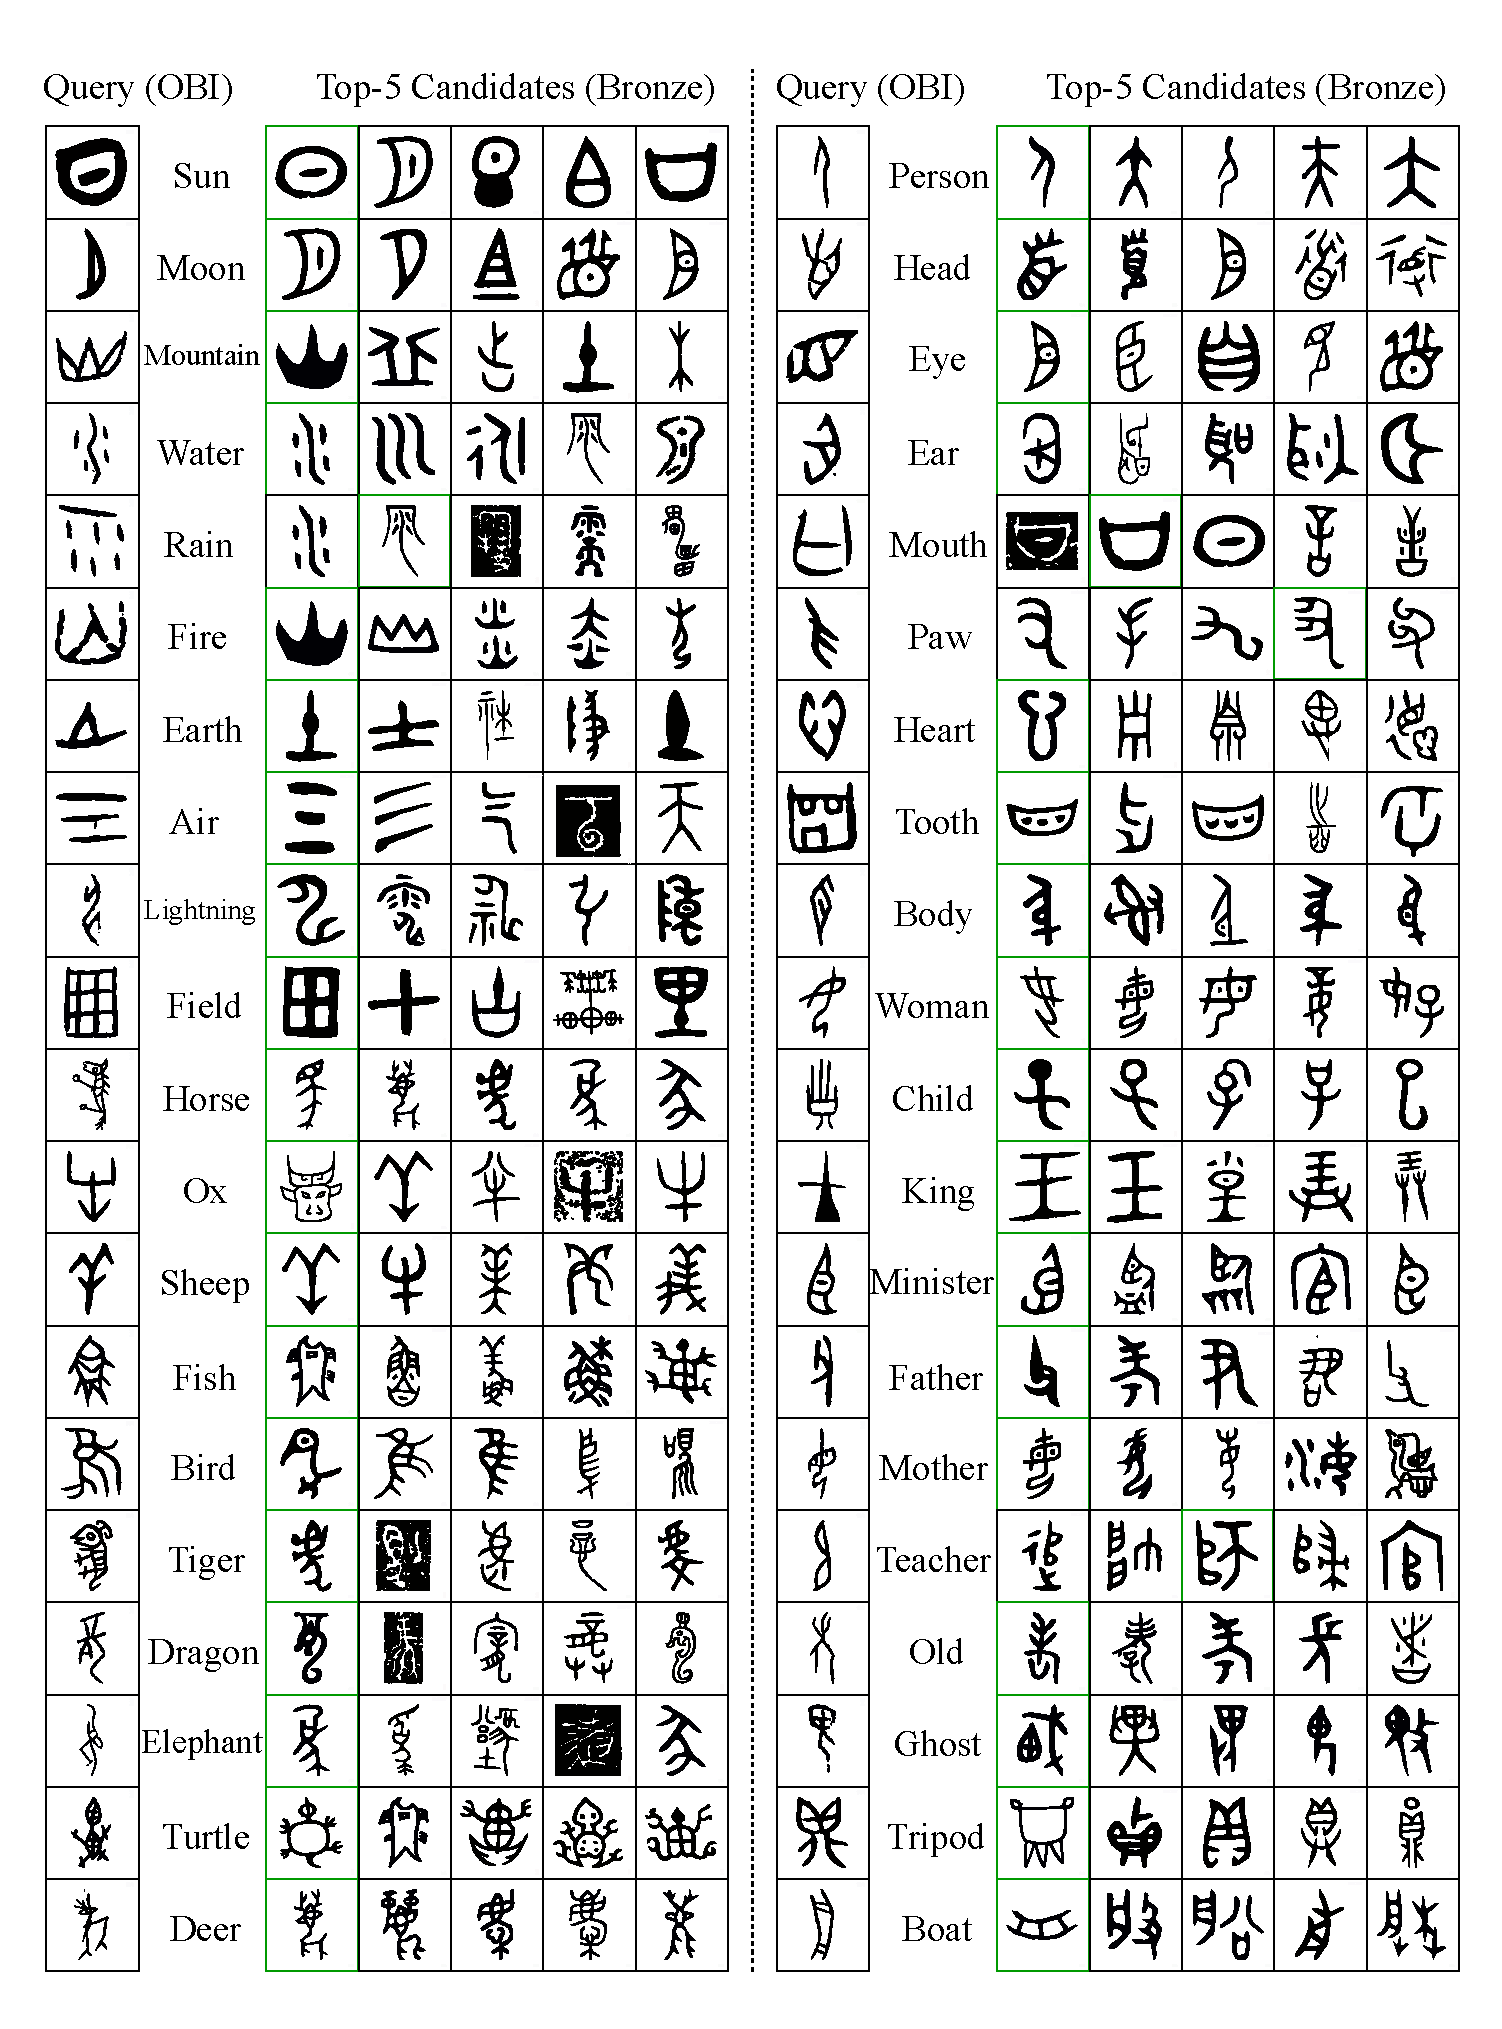
\includegraphics[width=0.93\textwidth]{gallery_full.pdf}
    \caption{\textbf{Comprehensive Retrieval Gallery.} This figure visualizes the Top-5 Bronze candidates retrieved for 40 representative OBI queries, arranged in two columns. The dataset spans diverse typologies, including Nature, Animals, Body Parts, People, and Artifacts. The \textcolor{green}{green box} indicates the ground truth. MSEF demonstrates robust retrieval capabilities, effectively distinguishing correct matches from visual and semantic distractors across different categories.}
    \label{fig:gallery_full}
\end{figure*}







\section{Manifold Neighborhood Visualization}
\label{app:neighborhood}

To empirically validate that our learned manifold captures meaningful linguistic topology rather than just memorizing training data, we visualize the local neighborhoods of characters in the latent space.

Figure~\ref{fig:manifold_vis} presents a \textbf{Manifold Neighborhood Visualization}. We randomly select 20 anchor points in the manifold space and visualize their 5 nearest neighbors. The visualization is divided into two panels to demonstrate cross-era consistency:
\begin{itemize}
    \item \textbf{Left Panel (OBI, $t=0$):} Shows the clustering in the Oracle Bone Inscription manifold. Note the high \textit{visual similarity} within clusters (e.g., characters sharing curved strokes or specific enclosed structures), reflecting the shape-based nature of the archaic script.
    \item \textbf{Right Panel (Bronze, $t=0.3$):} Shows the corresponding neighborhoods in the Bronze inscription manifold. Here, the clusters exhibit increased \textit{structural coherence}, often grouping characters with the same radicals or components.
\end{itemize}

This visualization confirms that MSEF maps semantically and visually related characters to proximate regions in the high-dimensional space. The transition from the OBI panel to the Bronze panel further illustrates how the manifold preserves these neighborhood structures (topology) even as the specific "representational vocabulary" (glyph style) evolves over time.

\begin{figure*}[h]
    \centering
    % 请确保您的图片文件名是 manifold_neighborhood.pdf
    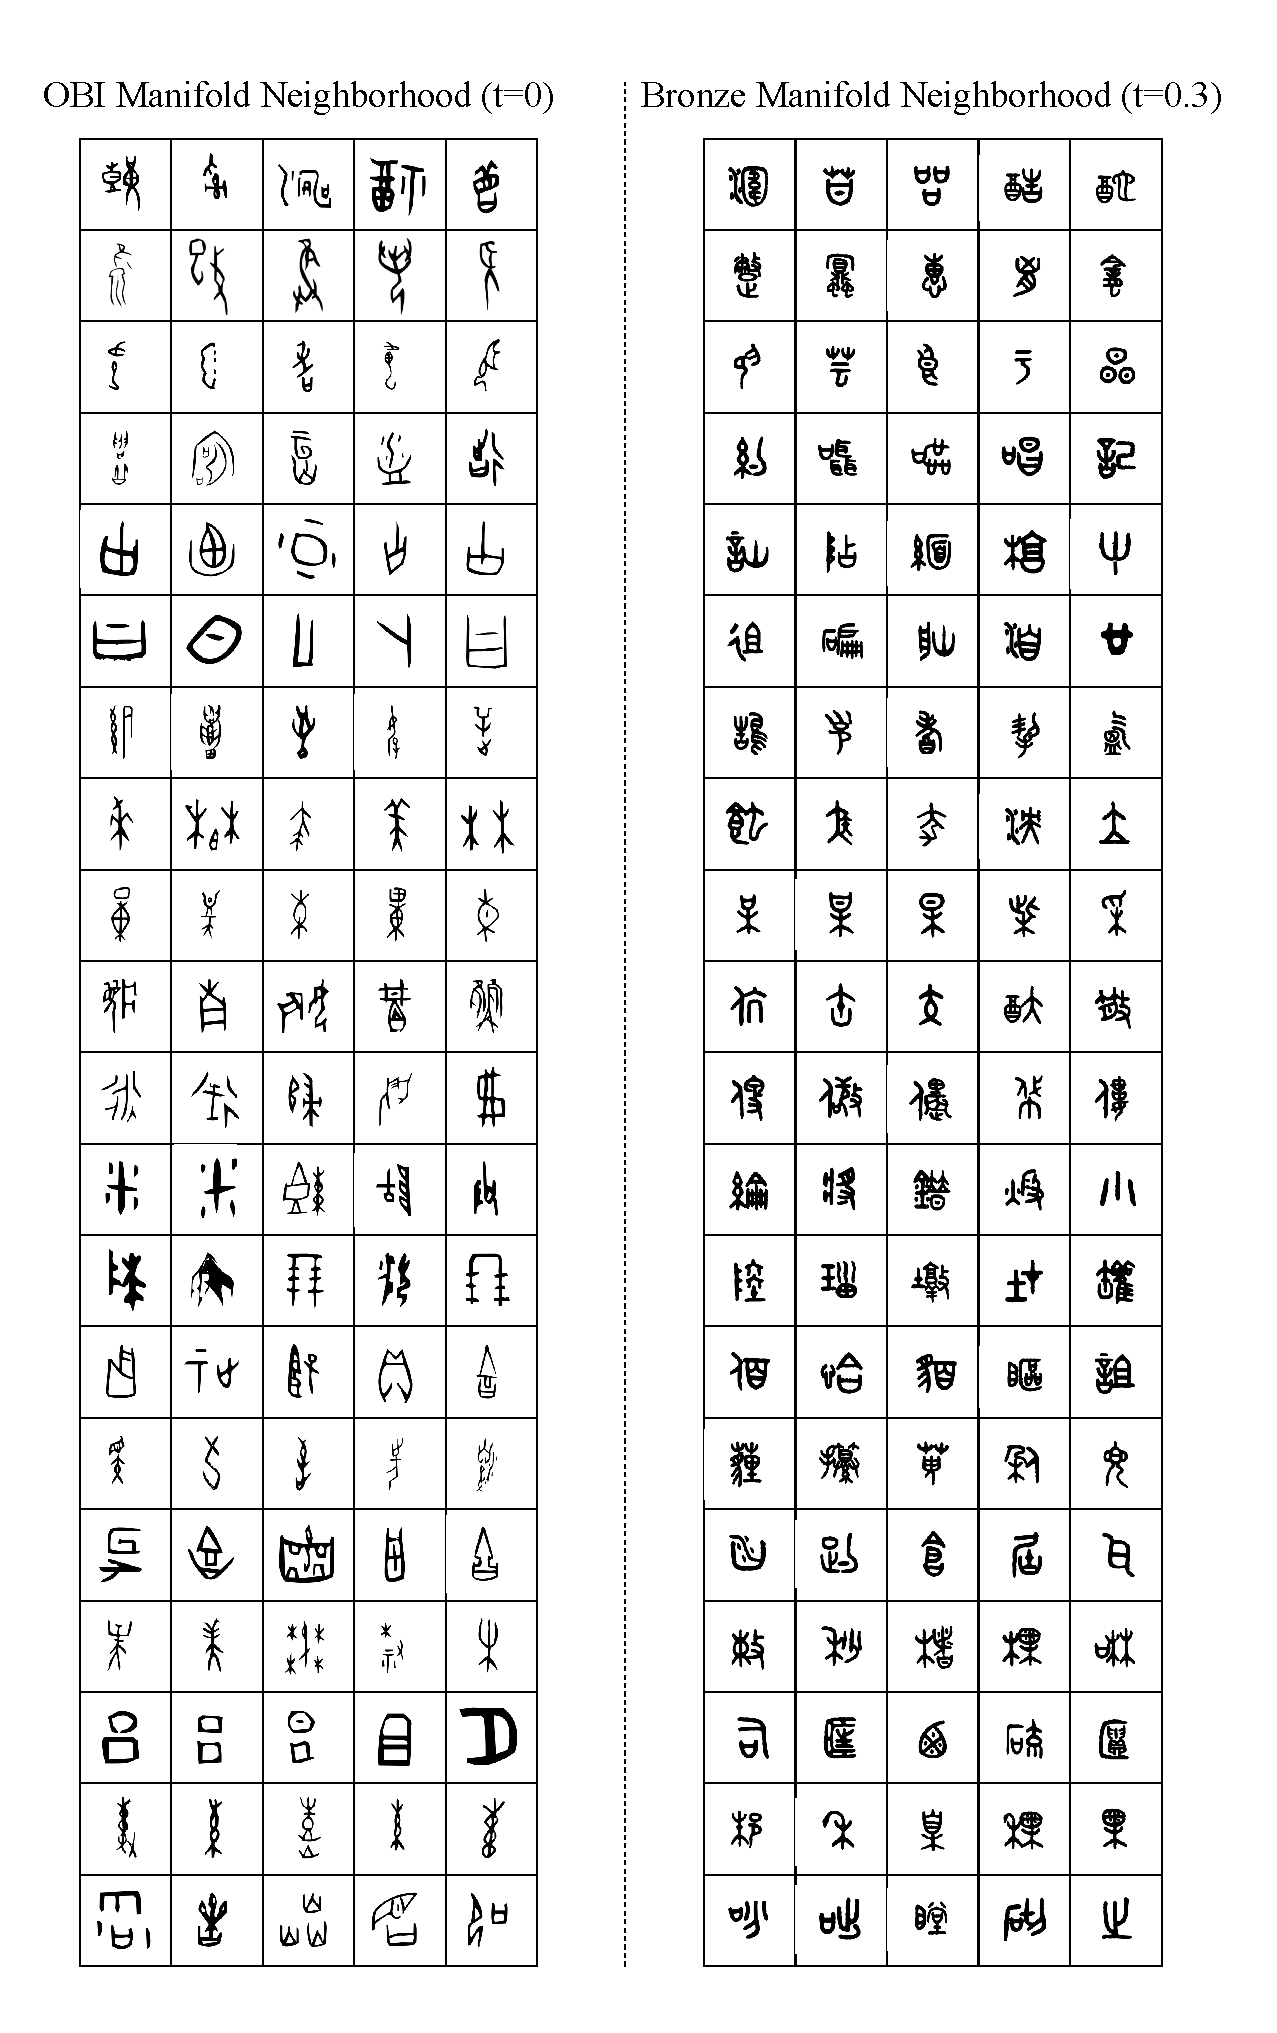
\includegraphics[width=0.77\textwidth]{manifold_neighborhood.pdf}
    \caption{\textbf{Manifold Neighborhood Visualization (Visual \& Semantic Similarity Clusters).} 
    We visualize the local manifold structure by querying 20 random anchor points and displaying their top-5 nearest neighbors in the feature space.
    \textbf{Left:} Neighborhoods in the OBI era ($t=0$). 
    \textbf{Right:} Neighborhoods in the Bronze era ($t=0.3$).
    Each row represents a distinct cluster. The dense clustering of visually similar (e.g., shape-based) and semantically related (e.g., radical-based) characters validates that the manifold successfully encodes the intrinsic geometric structure of Chinese script evolution.}
    \label{fig:manifold_vis}
\end{figure*}





\section{Fine-Grained Dataset Visualization}
\label{app:fine_grained_vis}

A core contribution of our work is the construction of a dataset with fine-grained temporal and regional annotations, distinct from prior works that rely on single representative glyphs per era.

Figure~\ref{fig:fine_grained_evolution} visualizes 20 representative evolution chains from our dataset. Unlike standard datasets, we preserve intra-era diversity:
\begin{itemize}
    \item \textbf{OBI (Scribal Groups):} We categorize Oracle Bone Inscriptions into eight distinct scribal groups: \textit{Dui} ($\mathcal{D}$), \textit{Bin} ($\mathcal{B}$), \textit{Li} ($\mathcal{L}$), \textit{Chu} ($\mathcal{C}$), \textit{He} ($\mathcal{H}$), \textit{Huang} ($\mathcal{H}u$), \textit{Zi} ($\mathcal{Z}$), and \textit{None} (indicating unclassified samples). This captures the stylistic variations across different diviner groups and periods within the Shang dynasty.
    \item \textbf{Bronze (Dynastic Sub-periods):} We trace evolution across six specific phases: \textit{Late Shang} (L.S), \textit{Early Western Zhou} (E.Z), \textit{Mid Western Zhou} (M.Z), \textit{Late Western Zhou} (L.Z), \textit{Spring \& Autumn} (Sp), and \textit{Warring States} (Wa). Note that for display clarity, sub-stages within Spring \& Autumn and Warring States are merged into their respective broader categories.
\end{itemize}

\begin{figure*}[h]
    \centering
    % 请确保您的图片文件名是 dataset_finegrained.pdf
    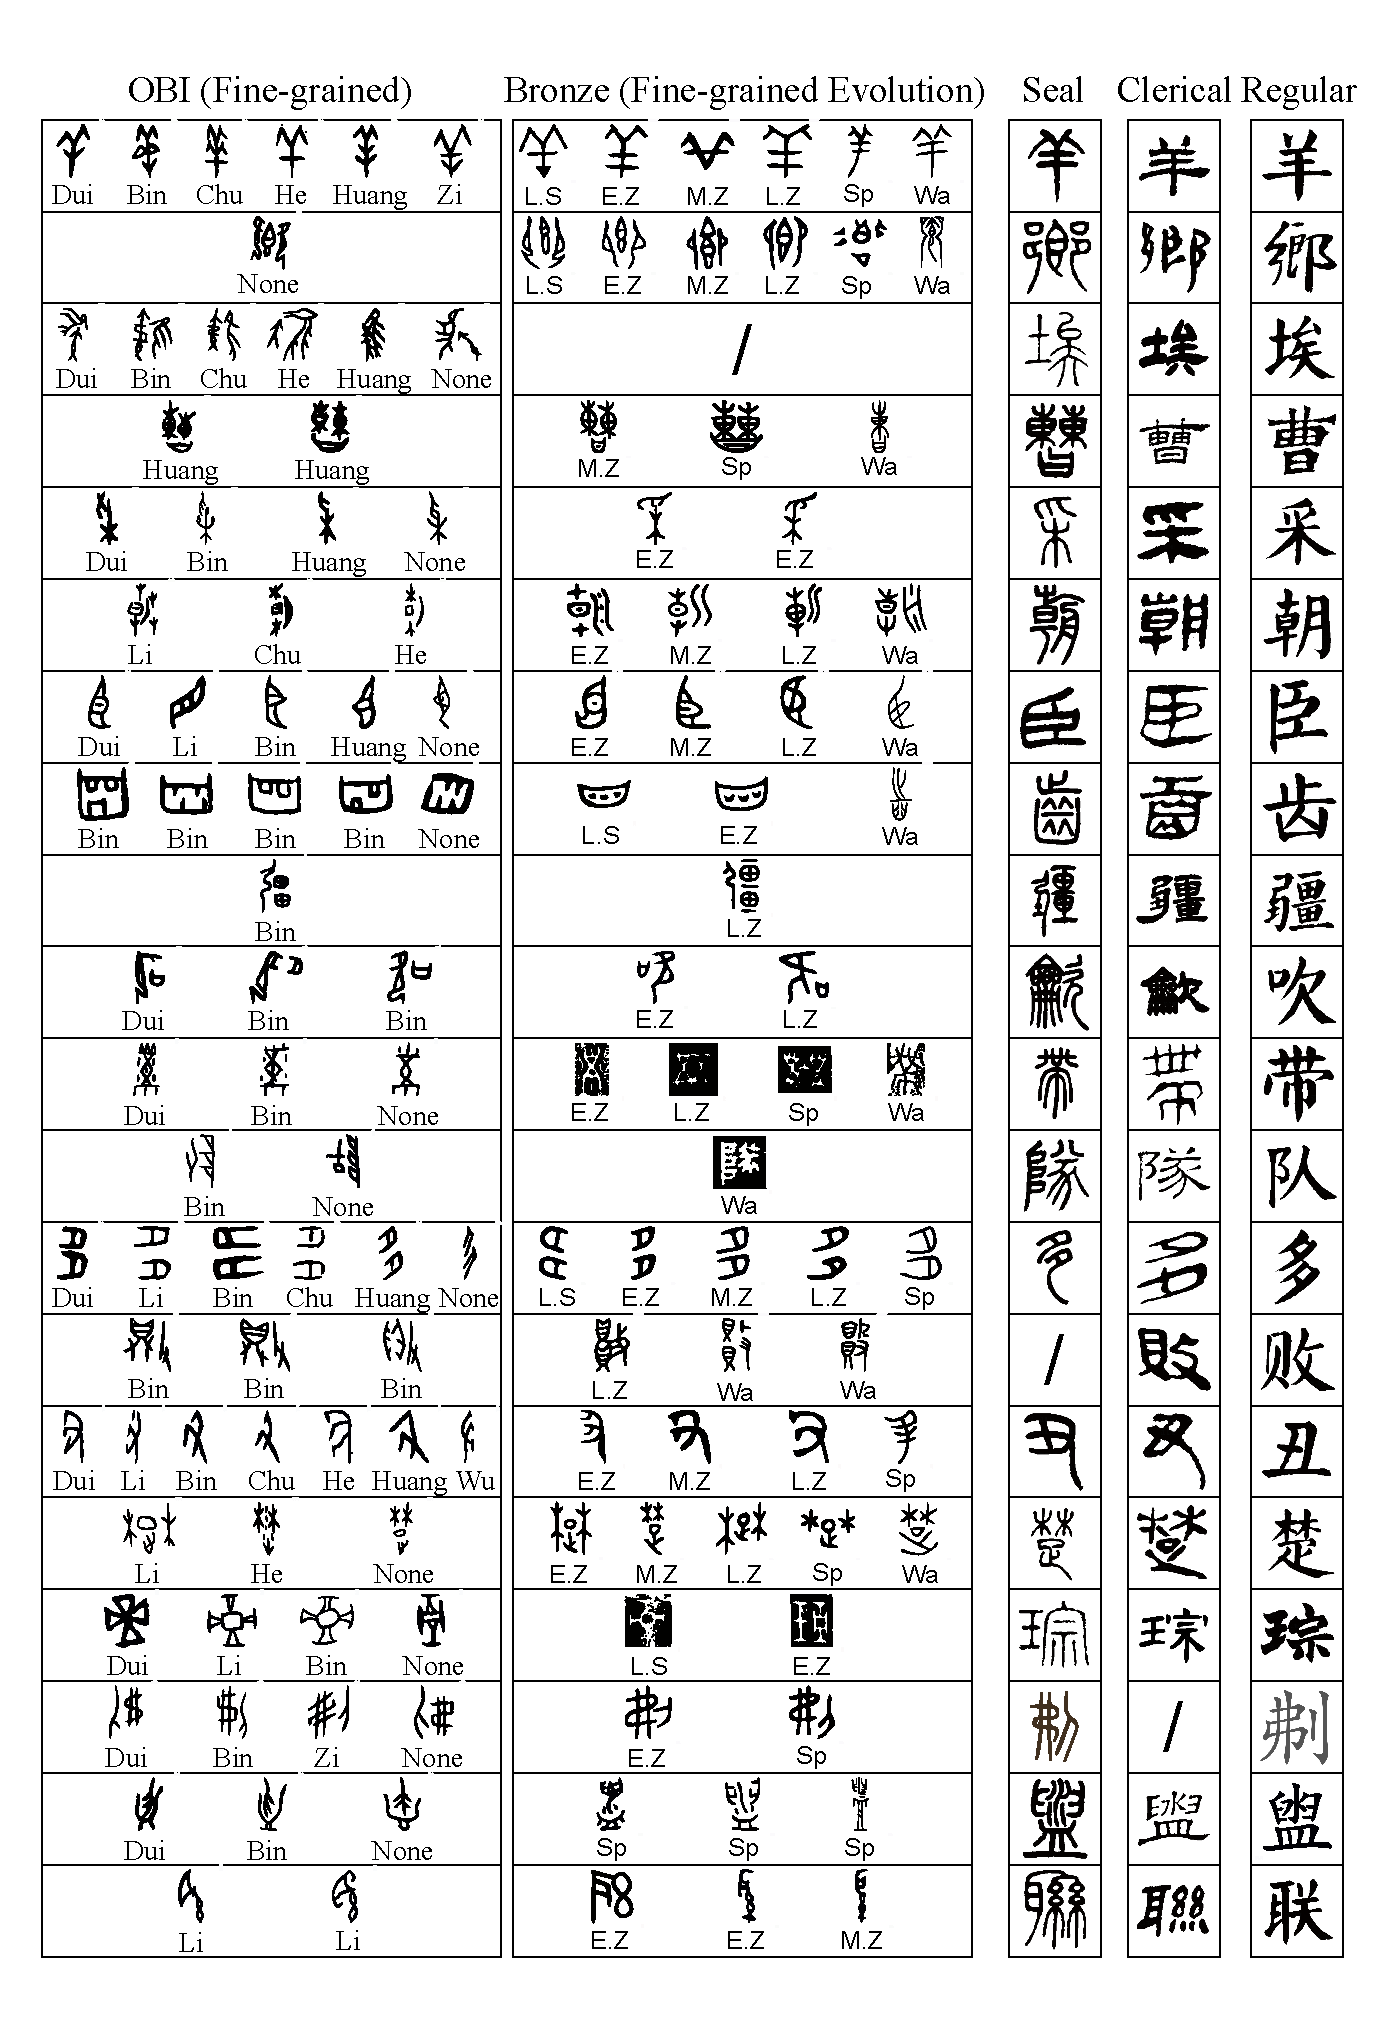
\includegraphics[width=0.85\textwidth]{dataset_finegrained.pdf}
    \caption{\textbf{Fine-Grained Evolutionary Trajectories.} 
    Visualization of 20 characters demonstrating the granular annotations in our dataset.
    \textbf{Left (OBI):} Variants are annotated by scribal groups (e.g., \textit{Bin}, \textit{Li}, \textit{Huang}).
    \textbf{Middle (Bronze):} Variants are annotated by sub-periods: \textbf{L.S} (Late Shang), \textbf{E.Z/M.Z/L.Z} (Early/Mid/Late Western Zhou), \textbf{Sp} (Spring \& Autumn), and \textbf{Wa} (Warring States).
    The symbol ``/'' indicates historical gaps where specific glyphs are not currently available in the excavated record.
    This granularity enables the model to learn subtle evolutionary shifts within eras, beyond coarse era-to-era transitions.}
    \label{fig:fine_grained_evolution}
\end{figure*}

%%%%%%%%%%%%%%%%%%%%%%%%%%%%%%%%%%%%%%%%%%%%%%%%%%%%%%%%%%%%

% \newpage
% \input{checklist.tex}

\FloatBarrier
\clearpage
\input{checklist.tex}

\end{document}